%% Préambule
\documentclass[10pt, french]{article}
% !TEX encoding = UTF-8 Unicode
% LaTeX Preamble for all cheatsheets
% Author : Gabriel Crépeault-Cauchon

% HOW-TO : copy-paste this file in the same directory as your .tex file, and add in your preamble the next command right after you have specified your documentclass : 
% \input{preamble-cheatsht.tex}
% ---------------------------------------------
% ---------------------------------------------

% Extra note : this preamble creates document that are meant to be used inside the multicols environment. See the documentation on internet for further information.

%% -----------------------------
%% Encoding packages
%% -----------------------------
\usepackage[utf8]{inputenc}
\usepackage[T1]{fontenc}
\usepackage{babel}
\usepackage{lmodern}
\usepackage[colorinlistoftodos]{todonotes}
%% -----------------------------
%% Variable definition
%% -----------------------------
\def\auteur{\href{https://github.com/ressources-act/Guide_de_survie_en_actuariat/blob/master/02_Cheatsheets/contributeurs/contributeurs-cheatshts.pdf}{\faGithub \ Liste des contributeurs}}
\def\BackgroundColor{white}
\usepackage{xargs} % for more logical new function creation

%% -----------------------------
%% Margin and layout
%% -----------------------------
% Determine the margin for cheatsheet
\usepackage[landscape, hmargin=1cm, vmargin=1.7cm]{geometry}
\usepackage{multicol}

% Remove automatic indentation after section/subsection title.
\setlength{\parindent}{0cm}

% Save space in cheatsheet by removing space between align environment and normal text.
\usepackage{etoolbox}
\newcommand{\zerodisplayskips}{%
  \setlength{\abovedisplayskip}{0pt}%
  \setlength{\belowdisplayskip}{0pt}%
  \setlength{\abovedisplayshortskip}{0pt}%
  \setlength{\belowdisplayshortskip}{0pt}}
\appto{\normalsize}{\zerodisplayskips}
\appto{\small}{\zerodisplayskips}
\appto{\footnotesize}{\zerodisplayskips}

%% -----------------------------
%% URL and links
%% -----------------------------
\usepackage{hyperref}
\hypersetup{colorlinks = true, urlcolor = gray!70!white, linkcolor = black}

%% -----------------------------
%% Document policy (uncomment only one)
%% -----------------------------
%	\usepackage{concrete}
	\usepackage{mathpazo}
%	\usepackage{frcursive} %% permet d'écrire en lettres attachées
%	\usepackage{aeguill}
%	\usepackage{mathptmx}
%	\usepackage{fourier} 

%% -----------------------------
%% Math configuration
%% -----------------------------
\usepackage[fleqn]{amsmath}
\usepackage{amsthm,amssymb,latexsym,amsfonts}
\usepackage{gensymb}
\usepackage{empheq}
\usepackage{numprint}
\usepackage{dsfont} % Pour avoir le symbole du domaine Z
%\usepackage{bigints} % pour des gros intégrales
% Mathematics shortcuts
\usepackage{scalerel,stackengine,amsmath}
\newcommand\equalhat{\mathrel{\stackon[1.5pt]{=}{\stretchto{%
    \scalerel*[\widthof{=}]{\wedge}{\rule{1ex}{3ex}}}{0.5ex}}}}
\newcommand{\reels}{\mathbb{R}}
\newcommand{\entiers}{\mathbb{Z}}
\newcommand{\naturels}{\mathbb{N}}
\newcommand{\eval}{\biggr \rvert}
\usepackage{cancel}
\newcommand{\derivee}[1]{\frac{\partial}{\partial #1}}
\newcommand{\prob}[1]{\Pr \left( #1 \right)}
\newcommand{\esp}[1]{\mathrm{E} \left[ #1 \right]} % espérance
\newcommand{\variance}[1]{\mathrm{Var} \left( #1   \right)}
\newcommand{\covar}[1]{\mathrm{Cov} \left( #1   \right)}
\newcommand{\laplace}{\mathcal{L}}
\newcommand{\deriv}[3][]{\frac{\partial^{#1}#3}{\partial #2^{#1}}}
\newcommand{\e}[1]{\mathrm{e}^{#1}}
\newcommand{\te}[1]{\text{exp}\left\{#1\right\}}
\DeclareMathSymbol{\shortminus}{\mathbin}{AMSa}{"39}
%%	Example usage:	\sumz{n}{i = 1} <=> \overset{n}{\underset{i = 1}{\sum}}
\newcommand{\sumz}[2]{\overset{#1}{\underset{#2}{\sum}}}
%%	Example usage:	\limz{h}{0} <=> \underset{h \rightarrow 0}{\lim}
\newcommand{\limz}[2]{\underset{#1 \rightarrow #2}{\lim}}
%%	Example usage:	\LVx{h}	<=>	\actsymb[h]{L}{}[]
%%					\LVx[n]{h}	<=>	\actsymb[h]{L}{}[n]
\newcommand{\LVx}[2][]{\actsymb[#2]{L}{}[#1]}
\DeclareMathOperator*{\argmax}{arg\,max}
\DeclareMathOperator*{\argmin}{arg\,min}
%%%	\icbox{<frame color>}{<background color>}{<text>}
\newcommandx{\icbox}[3][1 = bleudefrance, 2 = beaublue]{\fcolorbox{#1}{#2}{#3}}
%%	other good color combo is azure(colorwheel) arsenic
\usepackage{longfbox}
%	voir cette page, paquetage avec CSS https://ctan.math.illinois.edu/macros/latex/contrib/longfbox/longfbox.html
\newfboxstyle{rappel}{
	background-color = tealblue!20!white, 
	border-style = outset,
	breakable = true,
%	
	border-color = tealblue,
	border-radius = 1ex, 
%
	padding-bottom = 0.2ex,
	padding-top = 0.2ex,
	padding-left = 0.4ex,
	padding-right = 0.4ex,
%	
	border-top-width = 0.3ex,
	border-bottom-width = 0.3ex,
%
	border-left-width = 1ex, 
	border-bottom-left-radius = 0.2ex,
%	
	border-right-width = 1ex, 
	border-top-right-radius = 0.2ex,
%	
}
\newfboxstyle{formula}{ 
	background-color = beaublue, 
	border-color = bleudefrance
}
\newfboxstyle{imphl}{ 
	padding = 0pt,
	margin = 0pt,
	baseline-skip = false,
	background-color = palechestnut!60!white, 
	border-color = white
}
\newfboxstyle{conditions}{ 
	background-color = palechestnut, 
	border-color = red
}
\newcommandx{\rcbox}[3][1 = bleudefrance, 2 = beaublue]{\lfbox[border-radius = 0.5ex, background-color = #2, border-color = #1]{#3}}

% To indicate equation number on a specific line in align environment
\newcommand\numberthis{\addtocounter{equation}{1}\tag{\theequation}}

%
% Actuarial notation packages
%
\usepackage{actuarialsymbol}
\usepackage{actuarialangle}

%
% Matrix notation for math symbols (\bm{•})
%
\usepackage{bm}
% Matrix notation variable (bold style)
\newcommand{\matr}[1]{\mathbf{#1}}



%% -----------------------------
%% tcolorbox configuration
%% -----------------------------
\usepackage[most]{tcolorbox}
\tcbuselibrary{xparse}
\tcbuselibrary{breakable}

%%
%% Coloured box "definition" for definitions
%%
\DeclareTColorBox{definition}{ o }				% #1 parameter
{
	colframe=blue!60!green,colback=blue!5!white, % color of the box
	breakable, 
	pad at break* = 0mm, 						% to split the box
	title = {#1},
	after title = {\large \hfill \faBook},
}
%%
%% Coloured box "definition2" for definitions
%%
\DeclareTColorBox{definitionNOHFILL}{ o }				% #1 parameter
{
	colframe=blue!60!green,colback=blue!5!white, % color of the box
	pad at break* = 0mm, 						% to split the box
	title = {#1},
	before title = {\faBook \quad },
	breakable
}
%%
%% Coloured box "definition2" for definitions
%%
\DeclareTColorBox{definitionNOHFILLsub}{ o }				% #1 parameter
{
	colframe=blue!40!green,colback=blue!5!white, % color of the box
	pad at break* = 0mm, 						% to split the box
	title = {#1},
	before title = {\faNavicon \quad }, %faBars  faGetPocket
	breakable
}
%%
%% Coloured box "definition3" for propriétés
%%
\DeclareTColorBox{definitionNOHFILLprop}{ o }				% #1 parameter
{
	colframe=amber(sae/ece),colback=amber(sae/ece)!5!white, % color of the box
	pad at break* = 0mm, 						% to split the box
	title = {#1},
	before title = {\faGetPocket \quad }, %faBars  faGetPocket
	breakable
}
%%
%% Coloured box "definition3" for propriétés
%%
\DeclareTColorBox{definitionNOHFILLpropos}{ o }				% #1 parameter
{
	colframe=carmine,colback=carmine!5!white, % color of the box
	pad at break* = 0mm, 						% to split the box
	title = {#1},
	before title = {\faColumns \quad }, %\faEllipsisH  faColumns
	breakable
}


%%
%% Coloured box "algo" for algorithms
%%
\newtcolorbox{algo}[ 1 ]
{
	colback = blue!5!white,
	colframe = blue!75!black,
	title=#1,
	fonttitle = \bfseries,
	breakable
}
%%
%% Coloured box "conceptgen" for points adding to a concept's deifintion
%%
\newtcolorbox{conceptgen}[ 1 ]
{
	breakable,
	colback = beaublue,
	colframe = airforceblue,
	title=#1,
	fonttitle = \bfseries
}
%%
%% Coloured box "rappel" pour rappel de formules
%%
\DeclareTColorBox{conceptgen_enhanced}{ o }
{
	enhanced,
	title = #1,
	colback=beaublue, % color of the box
%	colframe=blue(pigment),
%	colframe=arsenic,	
	colbacktitle=airforceblue,
	fonttitle = \bfseries,
	breakable,
	boxed title style={size=small,colframe=arsenic} ,
	attach boxed title to top center = {yshift=-3mm,yshifttext=-1mm},
}
%%
%% Coloured box "probch3" pour formules relatives au 3ème chapitre de prob
%%
\newtcolorbox{probch3}[ 1 ]
{
	colback = ruddypink,
	colframe = burgundy,
	fonttitle = \bfseries,	
	breakable,
	title=#1
}
%%
%% Coloured box "formula" for formulas
%%
\newtcolorbox{formula}[ 1 ]
{
	colback = green!5!white,
	colframe = green!70!black,
	breakable,
	fonttitle = \bfseries,
	title=#1
}
%%
%% Coloured box "formula" for formulas
%%
\DeclareTColorBox{algo2}{ o }
{
	enhanced,
	title = #1,
	colback=blue!5!white,	
	colbacktitle=blue!75!black,
	fonttitle = \bfseries,
	breakable,
	boxed title style={size=small,colframe=arsenic} ,
	attach boxed title to top center = {yshift=-3mm,yshifttext=-1mm},
}
%%
%% Coloured box "examplebox" for formulas
%%
\newtcolorbox{examplebox}[ 1 ]
{
	colback = beaublue,
	colframe = amethyst,
	breakable,
	fonttitle = \bfseries,title=#1
}
%%
%% Coloured box "rappel" pour rappel de formules
%%
\newtcolorbox{rappel}[ 1 ]
{
	colback = ashgrey,
	colframe = arsenic,
	breakable,
	fonttitle = \bfseries,title=#1
}
%%
%% Coloured box "rappel" pour rappel de formules
%%
\DeclareTColorBox{rappel_enhanced}{ o }
{
	enhanced,
	title = #1,
	colback=ashgrey, % color of the box
%	colframe=blue(pigment),
%	colframe=arsenic,	
	colbacktitle=arsenic,
	fonttitle = \bfseries,
	breakable,
	boxed title style={size=small,colframe=arsenic} ,
	attach boxed title to top center = {yshift=-3mm,yshifttext=-1mm},
}
%%
%% Coloured box "notation" for notation and terminology
%%
\DeclareTColorBox{distributions}{ o }			% #1 parameter
{
	enhanced,
	title = #1,
	colback=gray(x11gray), % color of the box
%	colframe=blue(pigment),
	colframe=arsenic,	
	colbacktitle=aurometalsaurus,
	fonttitle = \bfseries,
	boxed title style={size=small,colframe=arsenic} ,
	attach boxed title to top center = {yshift=-3mm,yshifttext=-1mm},
	breakable
%	left=0pt,
%  	right=0pt,
%    box align=center,
%    ams align*
%  	top=-10pt
}
\newtcolorbox{contrib}[ 1 ]
{
	colback = babyblueeyes,
	colframe = airforceblue,
	fonttitle = \bfseries,
	title = {#1},
	valign = center
}

%% -----------------------------
%% Graphics and pictures
%% -----------------------------
\usepackage{graphicx}
\usepackage{pict2e}
\usepackage{tikz}

%% -----------------------------
%% insert pdf pages into document
%% -----------------------------
\usepackage{pdfpages}

%% -----------------------------
%% Color configuration
%% -----------------------------
\usepackage{color, soulutf8, colortbl}


%
%	Colour definitions
%
\definecolor{armygreen}{rgb}{0.29, 0.33, 0.13}	%	army
\definecolor{asparagus}{rgb}{0.53, 0.66, 0.42}	% pastel green militariesque
\definecolor{britishracinggreen}{rgb}{0.0, 0.26, 0.15}
\definecolor{calpolypomonagreen}{rgb}{0.12, 0.3, 0.17}
\definecolor{darkgreen}{rgb}{0.0, 0.2, 0.13}

\definecolor{antiquebrass}{rgb}{0.8, 0.58, 0.46}	% brown-ish light cardboard color

\definecolor{blue(munsell)}{rgb}{0.0, 0.5, 0.69}
\definecolor{blue(matcha)}{rgb}{0.596, 0.819, 1.00}
\definecolor{blue(munsell)-light}{rgb}{0.5, 0.8, 0.9}
\definecolor{bleudefrance}{rgb}{0.19, 0.55, 0.91}
\definecolor{blizzardblue}{rgb}{0.67, 0.9, 0.93}	%	mr.freeze light baby blue 
\definecolor{bondiblue}{rgb}{0.0, 0.58, 0.71}	%	darker cyan type inidgo blue
\definecolor{blue(pigment)}{rgb}{0.2, 0.2, 0.6}
\definecolor{bluebell}{rgb}{0.64, 0.64, 0.82}
\definecolor{airforceblue}{rgb}{0.36, 0.54, 0.66}
\definecolor{beaublue}{rgb}{0.74, 0.83, 0.9}    % almost white
\definecolor{blue_rectangle}{RGB}{83, 84, 244}		% ACT-2004
\definecolor{cobalt}{rgb}{0.0, 0.28, 0.67}	% nice light blue-ish
\definecolor{ballblue}{rgb}{0.13, 0.67, 0.8}	%	almost green ish blue ish
\definecolor{babyblueeyes}{rgb}{0.63, 0.79, 0.95}

\definecolor{indigo(web)}{rgb}{0.29, 0.0, 0.51}	% purple-ish
\definecolor{antiquefuchsia}{rgb}{0.57, 0.36, 0.51}	%	pastel matte (darkerish) purple ish
\definecolor{darkpastelpurple}{rgb}{0.59, 0.44, 0.84}	%	pretty purple
\definecolor{gray(x11gray)}{rgb}{0.75, 0.75, 0.75}
\definecolor{aurometalsaurus}{rgb}{0.43, 0.5, 0.5}
\definecolor{bulgarianrose}{rgb}{0.28, 0.02, 0.03}	%	dark maroon type 
\definecolor{pastelred}{rgb}{1.0, 0.41, 0.38}		%	light red pinktinybit ish
\definecolor{lightmauve}{rgb}{0.86, 0.82, 1.0}
\definecolor{eggshell}{rgb}{0.94, 0.92, 0.84}
\definecolor{azure(colorwheel)}{rgb}{0.0, 0.5, 1.0}
\definecolor{darkgreen}{rgb}{0.0, 0.2, 0.13}			
\definecolor{ao(english)}{rgb}{0.0, 0.5, 0.0}		% prertty apple dark pastel (light) green
\definecolor{green_rectangle}{RGB}{131, 176, 84}		% ACT-2004
\definecolor{red_rectangle}{RGB}{241,112,113}		% ACT-2004
\definecolor{amethyst}{rgb}{0.6, 0.4, 0.8}
\definecolor{amethyst-light}{rgb}{0.6, 0.4, 0.8}
\definecolor{ruddypink}{rgb}{0.88, 0.56, 0.59}

\definecolor{amber(sae/ece)}{rgb}{1.0, 0.49, 0.0} 	%	pretty orange ish
\definecolor{burntsienna}{rgb}{0.91, 0.45, 0.32}		%%	lighter pastel orange
\definecolor{burntorange}{rgb}{0.8, 0.33, 0.0}		%%	imilar but deeper orange
\definecolor{orange-red}{rgb}{1.0, 0.27, 0.0}

\definecolor{tealblue}{rgb}{0.21, 0.46, 0.53}

\definecolor{battleshipgrey}{rgb}{0.52, 0.52, 0.51}  % lilght ish gray
\definecolor{ashgrey}{rgb}{0.7, 0.75, 0.71}			% dark grey-black-ish
\definecolor{arsenic}{rgb}{0.23, 0.27, 0.29}			% light green-beige-ish gray
\definecolor{gray(x11gray)}{rgb}{0.75, 0.75, 0.75}

\definecolor{carmine}{rgb}{0.59, 0.0, 0.09} 			% deep red
\definecolor{amaranth}{rgb}{0.9, 0.17, 0.31}
\definecolor{brickred}{rgb}{0.8, 0.25, 0.33}
\definecolor{chestnut}{rgb}{0.8, 0.36, 0.36}		% pink red ish light
\definecolor{palechestnut}{rgb}{0.87, 0.68, 0.69}
\definecolor{pastelred}{rgb}{1.0, 0.41, 0.38}
\definecolor{forestgreen(traditional)}{rgb}{0.0, 0.27, 0.13}
%
% Useful shortcuts for coloured text
%
\newcommand{\orange}{\textcolor{orange}}
\newcommand{\red}{\textcolor{red}}
\newcommand{\cyan}{\textcolor{cyan}}
\newcommand{\blue}{\textcolor{blue}}
\newcommand{\green}{\textcolor{green}}
\newcommand{\purple}{\textcolor{magenta}}
\newcommand{\yellow}{\textcolor{yellow}}

%% -----------------------------
%% Enumerate environment configuration
%% -----------------------------
%
% Custum enumerate & itemize Package
%
\usepackage{enumitem}
%
% French Setup for itemize function
%
\frenchbsetup{StandardItemLabels=true}
%
% Change default label for itemize
%
\renewcommand{\labelitemi}{\faAngleRight}


%% -----------------------------
%% Tabular column type configuration
%% -----------------------------
\newcolumntype{C}{>{$}c<{$}} % math-mode version of "l" column type
\newcolumntype{L}{>{$}l<{$}} % math-mode version of "l" column type
\newcolumntype{R}{>{$}r<{$}} % math-mode version of "l" column type
\newcolumntype{f}{>{\columncolor{green!20!white}}p{1cm}}
\newcolumntype{g}{>{\columncolor{green!40!white}}m{1.2cm}}
\newcolumntype{a}{>{\columncolor{red!20!white}$}p{2cm}<{$}}	% ACT-2005
% configuration to force a line break within a single cell
\usepackage{makecell}


%% -----------------------------
%% Fontawesome for special symbols
%% -----------------------------
\usepackage{fontawesome}

%% -----------------------------
%% Section Font customization
%% -----------------------------
\usepackage{sectsty}
\sectionfont{\color{\SectionColor}}
\subsectionfont{\color{\SubSectionColor}}
\subsubsectionfont{\color{\SubSubSectionColor}}

%% -----------------------------
%% Footer/Header Customization
%% -----------------------------
\usepackage{lastpage}
\usepackage{fancyhdr}
\pagestyle{fancy}

%
% Header
%
\fancyhead{} 	% Reset
\fancyhead[L]{Aide-mémoire pour~\cours ~(\textbf{\sigle})}
\fancyhead[R]{\auteur}

%
% Footer
%
\fancyfoot{}		% Reset
\fancyfoot[R]{\thepage ~de~ \pageref{LastPage}}
\fancyfoot[L]{\href{https://github.com/ressources-act/Guide_de_survie_en_actuariat}{\faGithub \ ressources-act/Guide de survie en actuariat}}
%
% Page background color
%
\pagecolor{\BackgroundColor}




%% END OF PREAMBLE
% ---------------------------------------------
% ---------------------------------------------
\usepackage{array, multirow}
\usepackage{booktabs}
\usepackage{eurosym}
\setlist{leftmargin=*}

%% -----------------------------
%% Préambule
%% -----------------------------
\def\BackgroundColor{white}
\def\SectionColor{teal!90!black}
\def\SubSectionColor{teal!45!black}
\def\SubSubSectionColor{armygreen}
\def\cours{gestion du risque financier}
\def\sigle{ACT-2011 et ACT-1006}

%% -----------------------------
%% Section
%%	+	assure que les sections sont numérotées mais pas les sous-sections et plus tout en les mettant dans le TOC
%% -----------------------------
\setcounter{secnumdepth}{1}

%% -----------------------------
%% Début du document
%% -----------------------------
%%	Feuille basé sur 
\begin{document}
\begin{center}
	\textsc{\Large Contributeurs}\\[0.5cm] 
%	\hl{Pendant mon étude de IFM, je vais travailler sur cette feuille dans le dépôt de ressources-examens (https://github.com/ressources-act/Ressources-examens).}\\
%	\hl{Je vais la remettre ici au mois d'août.}
\end{center}
\begin{contrib}{ACT-2011\: Gestion des risques financiers II}
\begin{description}
	\item[aut.] Nicholas Langevin
	\item[aut.] Gabriel Crépeault-Cauchon 
	\item[aut., cre.] Alec James van Rassel
	\item[src.] Claire Bilodeau
	\item[src.] Thomas Landry	
	\item[src.]	Coaching Actuaries, Exam IFM Study Notes
	\item[pfr.]	Marc-André Devost
\end{description}
\end{contrib}


\newpage
\raggedcolumns

\part{Gestion des risques financiers II (ACT-2011)}
\begin{multicols*}{2}

\section{Introduction aux produits dérivés}

\begin{definitionNOHFILL}[Produits dérivés]
Titre financier dont sa valeur est déterminée par le prix de quelque chose d'autre, soit l'\textbf{actif sous-jacent} du produit dérivé.\\

Tout comme un couteau n'est pas dangereux de soi, les produits dérivés ne le sont pas non plus. On peut heurter quelqu'un avec un couteau tout comme on peut couper des patates. Le risque dépend de leur utilisation.\\

Les produits dérivés apparaissent souvent en raison d'une augmentation du risque du sous-jacent; ils sont en fait des \textbf{outils de gestion du risque}.
\end{definitionNOHFILL}

\begin{rappel_enhanced}[Origine]
Après 1971, le président Nixon a voulu défaire le standard de l'or (qui a causé de l'hyperinflation dans plusieurs pays) pour plutôt laisser le libre-marché fixer la valeur des devises de chaque pays.
\tcbline
\textbf{Causes} de la transformation des marchés:
\begin{itemize}[leftmargin = *]
	\item	Déréglementation;
	\item	Automatisation des traitements avec l'informatique;
	\item	Mondialisation.
\end{itemize}
\end{rappel_enhanced}

\begin{formula}{Exemples de produits dérivés}
\begin{itemize}[leftmargin = *]
	\item	Contrat à terme standardisé (\og \textit{futures contract} \fg{});
	\item	Contrat à terme de gré à gré (\og \textit{forward contract} \fg{});
	\item[]	\textit{Gré}: acceptation, ou consentement;
	\item	Option d'achat (\og \textit{call} \fg{});
	\item	Option de vente (\og \textit{put} \fg{});
	\item	Les \og \textit{\textbf{swaps}} \fg{}.
\end{itemize}
\end{formula} 

\begin{formula}{Exemples de sous-jacent aux produits dérivés}
\begin{multicols*}{2}
\begin{itemize}[leftmargin = *]
	\item	Indice boursier;
	\item	Taux d'intérêt;
	\item	Taux de change;
	\item	Climat;
	\item	Prix d'une marchandise.
\end{itemize}
\end{multicols*}
\end{formula} 

\begin{conceptgen}{Utilité}
\begin{itemize}[leftmargin = *]
	\item 	Gestion des risques (\textbf{hedging});
	\item[]	Par exemple, un avion peut se procurer une option d'achat pour contrer le risque d'une augmentation du prix du pétrole;
	\item[]	On dit qu'elle \og \textit{hedge} \fg{}, ou protège sa position, contre le prix du pétrole.
	\item 	\textbf{Spéculation};
	\item[]	Par exemple, un investisseur croit que le prix d'une action va augmenter et se procure une option d'achat.
	\item 	\textbf{Réduction} des \textbf{frais} de \textbf{transaction}: Faire le même profit qu'en transigeant des actions sans réellement les transiger;
	\item 	\textbf{Arbitrage} réglementaire: Éliminer le risque de posséder un actif en retenant ses privilèges.
	\item[]	Par exemple, un investisseur élimine le risque d'une action avec une option de vente tout en conservant ses droits de vote.
\end{itemize}
\end{conceptgen}

\begin{conceptgen}{Parties prenantes}
\begin{description}
	\item[Utilisateur final]	participant au contrat du produit dérivé;
		\begin{itemize}
		\item	\og \textit{end-user} \fg{}.
		\end{itemize}
	\item[\hypertarget{market_holder}{Teneur de marché}]	"crée" le marché en tant qu'intermédiaire;
		\begin{itemize}[leftmargin = *]
		\item	Il cherche à faire un profit, une "cote", sur la transaction;
		\item	\og \textit{Market-makers} \fg{}.
		\end{itemize}
	\item[Observateur économique]	observateurs du marché qui analysent et réglementent les activités des teneurs de marché et utilisateurs.
\end{description}
\end{conceptgen}

\begin{definitionNOHFILL}[Ingénierie financière] 
Création de produits dérivés à partir de d'autres produits.\\

\textbf{Implications}
\begin{itemize}[leftmargin = *]
	\item	Les teneurs de marchés peuvent \textbf{couvrir} leurs positions (\og \textit{hedging position} \fg{});
	\item	Les teneurs de marchés peuvent \textbf{personnaliser} les produits dérivés;
	\item	L'arbitrage réglementaire est difficile à empêcher puisqu'il existe souvent plusieurs façons pour recréer un produit dérivé.
		\begin{itemize}[leftmargin = *]
		\item	Pour comprendre le concept, $1 + 3 = 4$ tout comme $2 + 2$;
		\item	Si le numéro 3 est illégal, on peut arriver à 4 d'une autre façon.
		\end{itemize}		 
\end{itemize}
\end{definitionNOHFILL}

\columnbreak

\subsection{Marchés financiers}
\begin{definitionNOHFILL}[Transaction gré à gré] 
Transaction sans intermédiaire ou à l'extérieur de la bourse sur un marché hors cote. 

\begin{conceptgen}{Raisons pour ce type de transaction}
\begin{itemize}[leftmargin = *]
	\item Ce sont souvent de grosses transactions permettant d'économiser sur les frais de transaction;
	\item On peut combiner (sur une même transaction) plusieurs microtransactions et plusieurs types d'actifs.
\end{itemize}
\end{conceptgen}
\end{definitionNOHFILL}

\begin{algo2}[Étapes d'une transaction]
\begin{enumerate}
	\item 	L'acheteur et le vendeur se trouvent;
	\item 	On définit les obligations de chaque partie, on dit que la transaction est \og \textbf{cleared} \fg{};
		\begin{itemize}[leftmargin = *]
		\item	C'est-à-dire, l'actif à livrer, la date d'échéance, le prix, etc.;
		\item	Les transactions sur les marchés financiers sont \textit{cleared} avec un intermédiaire nommé la \textbf{chambre de compensation} (\og \textit{clearing house} \fg{});
		\item	Elle met en relation les acheteurs et vendeurs \textit{(1$^{\text{ère}}$ étape)}, et tient compte des obligations et paiements.
		\end{itemize}	
	\item 	La transaction a lieu et les obligations sont remplies par chaque partie, on dit que la transaction est \og \textit{settled} \fg{};
	\item 	Les registres de propriétés sont mis à jour.
\end{enumerate}	
\end{algo2}

\begin{definitionNOHFILL}[\textbf{Chambre de compensation} \og \textit{clearing house} \fg{}]
\begin{itemize}
	\item	La chambre de compensation règle beaucoup de transactions sur les marchés organisés;
	\item	Elle est une entité standardisée et réglementée;
	\item	\textbf{Novation} est défini comme un processus de substitution;
	\item	Dans le cas de produits dérivés, la chambre de compensation, \textit{par novation}, devient le vendeur de tous les acheteurs et l'acheteur de tous les vendeurs;
	\item	Donc, la chambre de compensation est un intermédiaire pour les acheteurs et vendeurs. 
\end{itemize}
\end{definitionNOHFILL}

\begin{conceptgen}{Mesures de taille et d'activité d'un marché}
\begin{description}
	\item[Volume total des transactions:] Nombre total de titres transigés pendant une période de temps donnée;
	\item[Valeur marchande:] Valeur de tout ce qui pourrait être transigé;
		\begin{itemize}[leftmargin = *]
		\item	$\text{nombre d'actions} \ \times \ \text{prix par action (\$)}$;
		\item	en anglais, le \og \textit{market value} \fg{};
		\item	Dans le cas des produits dérivés, ce n'est pas intéressant
		\end{itemize}
\tcbline
	\item[Valeur notionnelle:] Valeur du sous-jacent au produit dérivé;
	\item[Position ouverte:] Nombre de contrats pour lesquels un des parties a une obligation. 
		\begin{itemize}[leftmargin = *]
		\item	\og \textit{Open interest} \fg{}.
		\end{itemize}
%%%	-----number of contracts for which there is a future obligatioon for one party to perform
%%%	NOTE:
%%%	+	Du produit dérivé? 
%%%	+	Pas certain si c'est adéquat de définir de cette façon---i.e. restreinte au produit dérivé.
%%%	-----
\end{description}
\end{conceptgen}

Les compagnies recueillent du capital en émettant des actions et obligations selon leurs objectifs. 
\begin{description}
	\item[Obligations]	Une obligation se compare à un emprunt bancaire et est traitée comme de la dette;
		\begin{itemize}[leftmargin = *]
		\item	Souvent, elles sont émises pour des besoins de liquidité à court terme ou,
		\item	Pour le démarrage d'une entreprise.
		\end{itemize}
	\item[Actions]	Une action correspond à une partie de la compagnie.
		\begin{itemize}[leftmargin = *]
		\item	Souvent, une compagnie va faire une offre publique lorsqu'elle cherche, ou nécessite de l'argent pour soit s'élargir, développer de nouveaux produits, etc.;
		\item	L'avantage en comparaison à une obligation est qu'il n'y a pas de promesse de rembourser les fonds;
		\item	En revanche, la compagnie est forcée d'échanger une partie de son contrôle.
		\end{itemize}
\end{description}

Il s'ensuit que le \textbf{marché des actions} est plus actif (a un volume total de \textbf{transactions} plus important) que le \textbf{marché des obligations}; les obligations se transigent moins souvent que les actions. Cependant, la taille des deux marchés (valeur marchande) est similaire.\\

\textbf{Rôle des marchés financiers}: Partage du risque et diversification des risques. Si un risque est non diversifiable.\\

\begin{definitionNOHFILL}[\textbf{Écart acheteur-vendeur} \og \textit{Bid-Ask Spread} \fg{} ]
Écart entre le prix de vente (\textbf{ask}) et d'achat (\textbf{bid}).\\

Ceci correspond à la \textbf{marge de profit} que le teneur de marché conserve. En l'absence d'arbitrage, on aura $Ask - Bid > 0$.

\begin{conceptgen}{Prix}
\begin{description}
	\item[Ask:] Prix le plus \textit{élevé} auquel un investisseur est prêt à payer pour le sous-jacent;
		\begin{itemize}[leftmargin = *]
		\item	Lorsque le teneur de marché vend une action à un investisseur, il \textit{ask} le prix plus élevé;
		\item	\og \textit{ask price} \fg{} se traduit au \textbf{cours vendeur} représentant l'idée de regarder les prix auxquels se transigent l'actif.
		\end{itemize}
	\item[Bid:] Prix le plus \textit{faible} auquel un investisseur est prêt à vendre le sous-jacent.
		\begin{itemize}[leftmargin = *]
		\item	Lorsque le teneur de marché achète une action d'un investisseur, il \textit{bid} le prix plus faible;
		\item	\og \textit{bid price} \fg{} se traduit au \textbf{cours acheteur}.
		\end{itemize}
\end{description}

\end{conceptgen}

\end{definitionNOHFILL}

\begin{distributions}[Terminologie des marchés]
\begin{description}
	\item[Ordre au cours du marché:]	On achète et vend selon les meilleurs prix bid-ask actuels;
		\begin{itemize}[leftmargin = *]
		\item	\og \textit{Market order} \fg{}.
		\end{itemize}
	\item[Ordre à cours limité:] Ordre pour une quantité précise dans une tranche spécifiée de prix;
		\begin{itemize}[leftmargin = *]
		\item	\og \textit{Limit order} \fg{};
		\item	On achète le sous-jacent si $Ask < k$ ou on vend le sous-jacent si $Bid > k$ sinon aucune transaction a lieu.
		\end{itemize}
	\item[Ordre de vente stop:]	Ordre au cours du marché déclenché par l'atteinte d'un certain prix;
		\begin{itemize}[leftmargin = *]
		\item	\og \textit{Stop-loss order} \fg{};
		\item	On veut limiter sa perte si un sous-jacent perd énormément de valeur et le vendre si $Bid \leq k$.
		\end{itemize}
	\item[Longue] On se considère en position longue \textbf{par rapport au sous-jacent} si notre stratégie nous permet de bénéficier d'une \textcolor{ao(english)}{hausse} du sous-jacent;
		\begin{itemize}[leftmargin = *]
		\item	La position peut également être déterminé selon le produit dérivé; on se considère en position longue si l'on possède quelque-chose.
		\end{itemize}
	\item[Courte] On se considère en position longue \textbf{par rapport au sous-jacent} si notre stratégie nous permet de bénéficier d'une \red{baisse} du sous-jacent.
		\begin{itemize}[leftmargin = *]
		\item	La position peut également être déterminé selon le produit dérivé; on se considère en position longue si l'on emprunte quelque-chose.
		\end{itemize}
\end{description}
\end{distributions}

%%%	-----
%%	Pas assez pertinent pour l'inclure (AJVR-26/01/2020)
%%	Contrats ayant une protection pour chaque degrés en sur(sous) de 18 degrés celsius;
%\paragraph{Contrats saisonnales}
%\begin{description}
%	\item[cooling degree-day futures contracts:] Pour la rigueur de l'hiver (un froid anormalement élevé);
%	\item[heating degree-day futures contracts:] Pour la rigueur de l'été (une chaleur anormalement élevée);
%\end{description}
%%%	-----

\columnbreak
\subsection{Vente à découvert}

\begin{definitionNOHFILL}[Vente à découvert \og \textit{(short-sell)} \fg{}] 
La vente d'un actif qu'on ne possède pas. On peut y penser comme l'inverse d'un achat.\\

\begin{algo2}[Étapes d'une vente à découvert]
\begin{multicols*}{2}
\begin{enumerate}[leftmargin = *]
	\item[]	Au début:\\
	\item 	Emprunt d'un titre;
	\item	Vente du titre;
	\item[]	Après une certaine période de temps:
	\item	Achat du titre;
	\item	Remboursement du titre.
\end{enumerate}	
\end{multicols*}
\end{algo2}
\end{definitionNOHFILL}

\begin{formula}{Exemple de vente à découvert}
\begin{itemize}[leftmargin = *]
	\item	Mon ami James possède 5 actions d'Apple ayant chacune une valeur de 5\$;
	\item	Je lui emprunte ses 5 actions et lui promets d'y retourner;
	\item	Immédiatement, je revends ses actions sur le marché des actions;
		\begin{itemize}
		\item	Je ne suis pas inquiété, je suis certain que le prix va baisser;
		\item	Ce faisant, je suis certain que je serai capable de racheter ses actions plus tard à un prix plus faible.
		\end{itemize}
	\item	Après une certaine période de temps, j'achète 5 actions au nouveau prix et j’y retourne.
\end{itemize}
\end{formula}

\begin{conceptgen}{Raisons pour une vente à découvert}
\begin{itemize}[leftmargin = *]
	\item	\textbf{Spéculation}: Un investisseur tire profit d'une baisse de prix;
	\item	\textbf{Financement}: Une vente à découvert est une façon d'emprunter de l'argent;
	\item	\textbf{Couverture} (hedging): Un investisseur peut éliminer le risque d'une position longue sur une action avec une vente à découvert.
\end{itemize}
\end{conceptgen}

\begin{conceptgen}{Type de risques}
\begin{description}
	\item[Risque de défaut (de crédit)] Risque de ne pas être payé;
		\begin{itemize}[leftmargin = *]
		\item	Ce risque peut être réduit avec un dépôt initial en garantie ou une marge de sécurité;
		\item	\og \textit{credit risk} \fg{}.
		\end{itemize}	
	\item[Risque de rareté] Risque qu'il soit difficile de trouver un acheteur et un vendeur pour le sous-jacent.
		\begin{itemize}[leftmargin = *]
		\item	C'est le risque lié à un actif peu liquide;
		\item	En raison du faible nombre de transactions, il peut être difficile d'établir des clauses et conditions avec peu de transactions sur lesquelles se baser;
		\item	Il s'ensuit qu'il y a beaucoup de négociations et de variations dans les prix.
		\end{itemize}
\end{description}
\end{conceptgen}

\begin{conceptgen}{Frais}
L'\textbf{investisseur} est le \textit{short-seller} et le \textbf{prêteur} le \textit{détenteur des actions empruntées} par l'investisseur.

\begin{description}
	\item[\og \textit{short-sale \textbf{proceeds}} \fg{}]	Les recettes de la vente sont conservées comme collatéraux au cas où que l'investisseur ne retourne pas les actions;
		\begin{itemize}[leftmargin = *]
		\item	Soit le prêteur, ou un parti tiers, va conserver les revenus de la vente à découvert jusqu'au retour des actions;
		\item	À ce moment, elles seront retournées à l'investisseur.
		\end{itemize}
	\item[\og \textit{a \textbf{haircut}} \fg{}]	Marge de sécurité pour couvrir le risque que le prix des actions augmente trop pour que l'investisseur ait la capacité financière des retourner, le prêteur exige un \og dépôt \fg{} additionnel;
		\begin{itemize}[leftmargin = *]
		\item	Comme les recettes de la vente, cette marge de sécurité sera retournée au prêteur.
		\end{itemize}
	\item[\og \textit{Interest} \fg{}]	Il est naturel que le prêteur exige un retour sur la vente à découvert également;
		\begin{itemize}[leftmargin = *]
		\item	Dans le marché des actions, l'intérêt accumulé sur le collatéral est le \og \textit{short rebate} \fg{};
		\item	Dans le marché des obligations, c'est le \textbf{taux de mise en pension} (\og \textit{repo rebate} \fg{});
		\item	Ces taux sont habituellement \textit{plus faibles que} ceux du \textit{marché} et sont fondés sur l'offre et la demande.
		\end{itemize}
	\item[\og \textit{Dividends} \fg{}]	Il est possible que des dividendes soient payables lors du prêt;
		\begin{itemize}[leftmargin = *]
		\item	Puisque le détenteur de l'action sera celui à qui l'investisseur a vendu les actions, l'investisseur et le prêteur ne vont pas les recevoir;
		\item	Du point de vue du prêteur, les dividendes sont des paiements en espèce qu'il aurait reçus s'il n'avait pas prêté l'action;
		\item	Ce faisant, l'investisseur va payer ces dividendes au prêteur s'il y en a;
		\item	Pour le prêteur ils sont imposables alors que pour l'investisseur ils sont déductibles d'impôts;
		\item	Ce paiement se nomme le \textbf{taux de location} (\og \textit{lease rate} \fg{}) de l'actif.
		\end{itemize}
\end{description}
\end{conceptgen}

\newpage

\section{Introduction aux Forwards et aux options}

\begin{distributions}[Terminologie]
\begin{description}
	\item[Prime:] Prix payé pour un produit dérivé (à $t	=	0$).
		\begin{itemize}[leftmargin = *]
		\item	Dans le cas d'options, la prime correspond au coût ;
		\item	Si \textcolor{blue}{positif}, il s'agit d'un \textbf{coût} ;
		\item	Si \textcolor{red}{négatif}, il s'agît d'une \textbf{compensation}.		
		\end{itemize}
	\item[Valeur à l'échéance $T$:]	L'argent que l'on reçoit à l'échéance.
		\begin{itemize}[leftmargin = *]
		\item	En anglais, \og \textit{payoff} \fg{} ;
		\item	C'est à dire, les flux de trésorier au temps $t = T$.
		\end{itemize}
	\item[Profit] 
		= (valeur à l'échéance) - (valeur accumulée du coût initial) \\
		= $VA$(flux monétaires)\footnote{\textbf{V}aleur \textbf{A}ccumulée au taux sans risque.}
		\begin{itemize}[leftmargin = *]
		\item	Le profit soustrait les flux financiers initiaux accumulés de la valeur à l'échéance;
		\item	Par exemple, acheter une voiture et la revendre 10 ans plus tard:
			\begin{align*}
			\text{profit} 
			=	&\text{(prix de revente dans 10 ans)} -\\ &\text{\shortstack{(valeur accumulée, au courant des 10 dernières années,\\ du coût d'achat initial (à $t = 0$) )}}
			\end{align*}
		\item	Dans le cas d'options, on soustrait la valeur accumulée de la prime.
		\end{itemize}
	\tcbline
	\item[$\delta$]	Taux de dividendes composé continûment.
	\item[$r_{f}$] 	\textcolor{amethyst}{force} (\textcolor{teal}{taux}) d'intérêt sans risque \textcolor{amethyst}{composé continûment} (\textcolor{teal}{effectif annuel});
	\item[$T$]	date d'échéance.
\end{description}
\end{distributions}

\begin{definitionNOHFILLprop}[\og \textit{Cost of carry} \fg{}]
On peut interpréter l'écart entre le taux sans risque $r_{f}$ et le taux de dividende $\delta$ d'une action comme le \og \textit{cost of carry} \fg{}	=	$r_{f}	-	\delta$.
\end{definitionNOHFILLprop}

\columnbreak

\subsection{Contrats à terme de gré à gré}
\begin{definitionNOHFILL}[Contrat à terme (de gré à gré) \og \textit{forward contract} \fg{}]
Contrat selon lequel: 
\begin{itemize}
	\item	\textit{deux} partis s'\textbf{engagent} d'\textbf{échanger}---un à \textit{acheter} et l'autre à \textit{vendre};
	\item	une \textit{certaine} \textbf{quantité} d'un \textit{certain} \textbf{bien}---l'actif sous-jacent $S$;	
	\item	à un \textit{certain} \textbf{prix}---prix à terme $F_{0, T}$;
	\item	à un \textit{certain} \textbf{endroit} à une \textit{certaine} \textbf{date}---date d'échéance, $T$;
\end{itemize}

L'engagement est au départ à $t = 0$ mais aucune transaction y a lieu. Ce faisant, le profit sera égal à la valeur à l'échéance puisqu'il n'a pas de flux financiers à 0 à accumuler. L'achat \textbf{ferme} en revanche, implique l'\textit{achat} et la livraison de l'actif au départ à $t = 0$. Donc:
\begin{center}
\begin{tabular}{|	>{\columncolor{airforceblue}}c	| >{\columncolor{beaublue}}c | >{\columncolor{beaublue}}c  |}
\hline\rowcolor{airforceblue} 
\textcolor{white}{\textbf{Transaction}}	&	\textcolor{white}{\textbf{Valeur à l'échéance}}	&	\textcolor{white}{\textbf{Profit}}		\\\specialrule{0.1em}{0em}{0.0em} 
\textcolor{white}{Achat ferme}				&	$S_{T}$	&	$S_{T} - S_{0} \textrm{e}^{rT}$	\\\hline
\textcolor{white}{Contrat à terme (achat)}	&	$S_{T} - F_{0, T}$	&	$S_{T} - F_{0, T}$	\\\hline
\end{tabular}
\end{center}
\end{definitionNOHFILL}

\begin{distributions}[Notation de prix]
\begin{description}
	\item[$S_{t}$:] \textbf{Valeur} de l'actif \textbf{s}ous-jacent à $t$;
	\item[$S_{0}$:] \textbf{Prix au comptant};
		\begin{itemize}[leftmargin = *]
		\item	\og \textit{(spot price)} \fg{};
		\item	C'est le paiement pour la livraison immédiate à $t = 0$;
		\item	En d'autres mots, le prix de l'actif sous-jacent aujourd'hui payable dans le cas d'un achat ferme.
		\end{itemize}
	\item[$F_{0, T}$:]	\textbf{Prix à terme} payable à $T$;
		\begin{itemize}[leftmargin = *]
		\item	$F_{0, T} = S_{0} \textrm{e}^{r (T - 0)}$
		\end{itemize}
	\item[$F_{0, 0}$:]	est nul.
\end{description}
La notation $F_{0, T}$ vient de \og \textit{future} \fg{} ou \og \textit{forward} \fg{}.
\end{distributions}

\begin{formula}{Exemple de bateau}
\begin{itemize}[leftmargin = *]
	\item	Je veux acheter un \textit{(quantité)} bateau \textit{(bien)}, mais il est inconvénient pour moi de le recevoir maintenant;
	\item	En lieu, puisque je veux l'acheter maintenant, je signe une entente \textit{(engagement)} pour l'acheter;
	\item	La seule différence entre l'acheter aujourd'hui \textit{(au prix au comptant $S_{0}$)} et l'acheter lorsque la neige fond \textit{(au prix à terme $F_{0, T}$)} est l'accumulation d'intérêt;
	\item	Puisqu'on suppose tout les deux d'êtres fiables et sans risque, le prix est accumulé au taux sans risque ($r$) et le prix payable rendu à l'été ($T$) sera $F_{0, T} = S_{0} \textrm{e}^{r (T - 0)}$;
	\item[]	Si le taux sans risque est un \textbf{taux} \textbf{plutôt} qu'une \textit{force} d'intérêt, on obtient $F_{0, T} = S_{0} (1 + r_f)^{T}$.
\end{itemize}
\end{formula}

\subsection{Options}

\begin{definitionNOHFILL}[Exercice (levée)]
Décision d'\textit{exercer} l'option d'achat ou de vente.

\begin{distributions}[Notation]
\begin{itemize}[leftmargin = *]
	\item[$K$:]	\textbf{Prix d'exercice} \textit{(\textbf{strike price})};
\end{itemize}
\end{distributions}

\begin{conceptgen}{Types d'exercices}
\begin{description}
	\item[\textbf{\underline{E}}uropéen:]		\textbf{Au moment} d'\textbf{\underline{e}}xpiration de l'option $T$;
	\item[\textbf{\underline{A}}méricain:]	\textbf{N'importe quand} (\textbf{\underline{a}}ny moment) d'ici $T$;
	\item[\textbf{\underline{B}}ermudien:]	À \textbf{quelques périodes} (\textbf{\underline{b}}ounded periods) d'ici $T$;
\end{description}
En réalité, la \textit{majorité des options sont américaines}.
\end{conceptgen}
\end{definitionNOHFILL}

\begin{definitionNOHFILL}[Obligation zéro coupon]
\begin{minipage}{0.6\columnwidth}
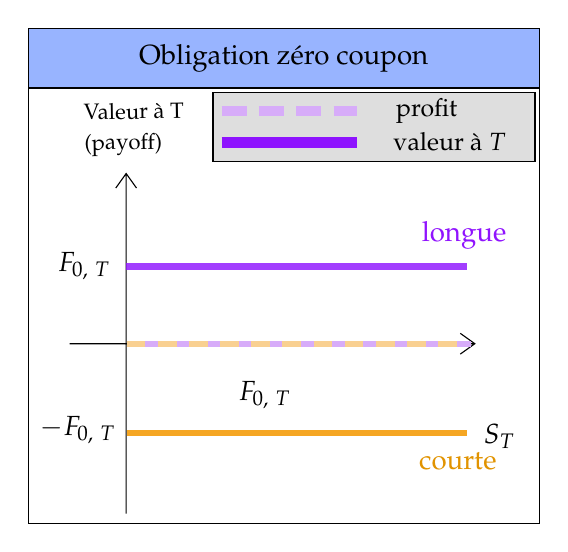
\begin{tikzpicture}[x=0.75pt,y=0.75pt,yscale=-1,xscale=1]
%uncomment if require: \path (0,300); %set diagram left start at 0, and has height of 300

%Shape: Axis 2D [id:dp5760713807677853] 
\draw  (68,203.33) -- (263.17,203.33)(95.17,121.33) -- (95.17,285.17) (256.17,198.33) -- (263.17,203.33) -- (256.17,208.33) (90.17,128.33) -- (95.17,121.33) -- (100.17,128.33)  ;
%Straight Lines [id:da14694919423796993] 
\draw [color={rgb, 255:red, 245; green, 166; blue, 35 }  ,draw opacity=1 ][line width=2.25]    (95.5,246.33) -- (259.5,246.33) ;


%Straight Lines [id:da006960924907699395] 
\draw [color={rgb, 255:red, 142; green, 19; blue, 254 }  ,draw opacity=0.82 ][line width=2.25]    (95.25,166.08) -- (259.5,166.08) ;


%Shape: Rectangle [id:dp6904794669628107] 
\draw   (48,51.33) -- (294.17,51.33) -- (294.17,290) -- (48,290) -- cycle ;
%Shape: Rectangle [id:dp19849032343228457] 
\draw  [fill={rgb, 255:red, 152; green, 180; blue, 255 }  ,fill opacity=1 ] (48,51.33) -- (294.17,51.33) -- (294.17,80.13) -- (48,80.13) -- cycle ;
%Straight Lines [id:da7331693440860174] 
\draw [color={rgb, 255:red, 215; green, 172; blue, 249 }  ,draw opacity=1 ][line width=2.25]  [dash pattern={on 6.75pt off 4.5pt}]  (102.5,203.33) -- (262.5,203.33) ;


%Straight Lines [id:da37881158739253507] 
\draw [color={rgb, 255:red, 249; green, 208; blue, 145 }  ,draw opacity=1 ][line width=2.25]  [dash pattern={on 6.75pt off 4.5pt}]  (95.5,203.33) -- (260.33,203.33) ;


%Shape: Rectangle [id:dp7574038380258179] 
\draw  [fill={rgb, 255:red, 222; green, 222; blue, 222 }  ,fill opacity=1 ] (137,82.33) -- (292.17,82.33) -- (292.17,115.33) -- (137,115.33) -- cycle ;
%Straight Lines [id:da663902422463923] 
\draw [color={rgb, 255:red, 215; green, 172; blue, 249 }  ,draw opacity=1 ][line width=3.75]  [dash pattern={on 9pt off 4.5pt}]  (141.17,91.33) -- (206.17,91.33) ;


%Straight Lines [id:da012272169443842351] 
\draw [color={rgb, 255:red, 142; green, 19; blue, 254 }  ,draw opacity=1 ][line width=3.75]    (141.17,106.33) -- (206.17,106.33) ;


% Text Node
\draw (275,248) node   [align=left] {$\displaystyle S_{T}$};
% Text Node
\draw (75,166) node   [align=left] {$\displaystyle F_{0,\ T}$};
% Text Node
\draw (72,245) node   [align=left] {$\displaystyle -F_{0,\ T}$};
% Text Node
\draw (99,100) node  [font=\small,rotate=-358.99] [align=left] {{\footnotesize Valeur à T }\\{\footnotesize (payoff)}};
% Text Node
\draw (162,228) node   [align=left] {$\displaystyle F_{0,\ T}$};
% Text Node
\draw (171.08,65.73) node   [align=left] {Obligation zéro coupon};
% Text Node
\draw (255,260) node  [color={rgb, 255:red, 225; green, 147; blue, 0 }  ,opacity=1 ] [align=left] {courte};
% Text Node
\draw (258,151) node  [color={rgb, 255:red, 144; green, 19; blue, 254 }  ,opacity=1 ] [align=left] {longue};
% Text Node
\draw (251,106) node  [font=\small] [align=left] {valeur à $\displaystyle T$};
% Text Node
\draw (240,91) node  [font=\small] [align=left] {profit};

\end{tikzpicture}
\end{minipage}
\begin{minipage}{0.4\columnwidth}
La position 
\begin{description}
	\item[longue]	Équivaut à un dépôt;
	\item[courte]	Équivaut à un emprunt.
\end{description}
\begin{center}
\begin{tabular}{| >{\columncolor{beaublue}}c |}
\hline\rowcolor{airforceblue} 
	\textcolor{white}{\textbf{Valeur à l'échéance}}	\\\specialrule{0.1em}{0em}{0.0em} 
$F_{0, T}$	\\\hline
\hline\rowcolor{airforceblue} \textcolor{white}{\textbf{Profit}} \\\specialrule{0.1em}{0em}{0.0em} 
$F_{0, T} - (F_{0, T} - \textrm{e}^{-rT}) \textrm{e}^{rT}$	\\\hline
\end{tabular}
\end{center}
\end{minipage}

Le profit sera donc toujours nul.
\end{definitionNOHFILL}


\begin{definitionNOHFILL}[Option d'achat]
Contrat qui: 
\begin{itemize}[leftmargin = *]
	\item	\textit{permet} \textbf{(optionnel)} à son \textit{détenteur} \textbf{d'acheter};
	\item	une \textit{certaine} \textbf{quantité} d'un \textit{certain} \textbf{bien}---l'actif sous-jacent;	
	\item	à un \textit{certain} \textbf{prix}---prix d'exercice $K$;
	\item	à un \textit{certain} \textbf{endroit} à, ou d'ici, une \textit{certaine} \textbf{date}---date d'échéance, $T$;
\end{itemize}

\begin{distributions}[Notation]
\begin{description}
	\item[$C_{0}$]	\textbf{Prix} pour acheter l'option d'achat;
	\item[$C(K)$]	Notation pour représenter l'option d'achat (\og \textit{\textbf{C}all} \fg{}) avec un prix d'exercice de $K$.
\end{description}
En réalité, on dénote le prix, alias prime, avec $C(K)$ mais selon la notation de Claire elle aime le faire avec $C_{0}$.
\end{distributions}
\end{definitionNOHFILL}

\begin{definitionNOHFILL}[Option de vente]
Contrat qui \textit{permet} à son \textit{détenteur} de \textbf{vendre} au lieu d'acheter.

\begin{distributions}[Notation]
\begin{description}
	\item[$P_{0}$]	\textbf{Prix} pour acheter l'option de vente;
	\item[$P(K)$]	Notation pour représenter l'option de vente (\og \textit{\textbf{P}ut} \fg{}) avec un prix d'exercice de $K$.
\end{description}
En réalité, on dénote le prix, alias prime,  avec $P(K)$ mais selon la notation de Claire elle aime le faire avec $P_{0}$.
\end{distributions}

\paragraph*{Note}	L'acheteur d'une option de vente a une position \textbf{longue} par rapport à l'\textbf{option} mais une position \textbf{courte} par rapport au \textbf{sous-jacent}.

%%%	------	
%%%	Commencé à convertir le tableau pour être du même format que la boite de l'obligation;
%%%	Pense pas par contre que ce sera aussi beau donc je laisse tel quel;
%\begin{minipage}{0.6\columnwidth}
%
%\end{minipage}
%\begin{minipage}{0.4\columnwidth}
%La position 
%\begin{center}
%\begin{tabular}{|	>{\columncolor{airforceblue}}m{1.2cm}	| >{\columncolor{beaublue}}r |}
%\hline\rowcolor{airforceblue} 
%\textcolor{white}{\textbf{Position}}	&	\textcolor{white}{\textbf{Valeur à l'échéance}}	\\\specialrule{0.1em}{0em}{0.0em} 
%\textcolor{white}{Longue}	&	$\max\{0, K - S_{T}\}$	\\\hline
%\textcolor{white}{Courte}	&	$\textcolor{burntsienna}{\boldsymbol{-}}\max\{0, K - S_{T}\}$	\\\hline
%\hline\rowcolor{airforceblue} 
%\textcolor{white}{\textbf{Position}}	&\textcolor{white}{\textbf{Profit}} \\\specialrule{0.1em}{0em}{0.0em} 
%\textcolor{white}{Longue}	&	$\max\{0, K - S_{T}\} - AV(\text{primes})$	\\\hline
%\textcolor{white}{Courte}	&	$\textcolor{burntsienna}{\boldsymbol{-}}\max\{0, K - S_{T}\} + AV(\text{primes})$	\\\hline
%\end{tabular}
%\end{center}
%\end{minipage}
%%%	------	
\end{definitionNOHFILL}

\begin{center}
	Profit (perte) extrême
	
\begin{tabular}{| >{\columncolor{beaublue}}c |	c	|	c	|}
\hline\rowcolor{airforceblue} 
	\textcolor{white}{\textbf{Position}}	&	\textcolor{white}{\textbf{Minimum}}	&	\textcolor{white}{\textbf{Maximum}}\\\specialrule{0.1em}{0em}{0.0em} 
Contrat à terme (longue)	&	$-F_{0, T}$						&	$+\infty$	\\
Contrat à terme (courte)	&	$-\infty$						&	$+F_{0, T}$	\\\hline
Option d'achat (longue)	&	$-C_{0}\textrm{e}^{rT}$			&	$+\infty$	\\
Option d'achat (courte)	&	$-\infty$						&	$+C_{0}\textrm{e}^{rT}$	\\\hline
Option de vente (longue)	&	$-P_{0}\textrm{e}^{rT}$			&	$K - P_{0}\textrm{e}^{rT}$	\\
Option de vente (courte)	&	$-(K - P_{0}\textrm{e}^{rT})$	&	$+P_{0}\textrm{e}^{rT}$	\\\specialrule{0.1em}{0em}{0.0em} 
\end{tabular}
\end{center}

\paragraph{Types de positions:}
\begin{description}
	\item[Position capitalisée]	Une position est dite "capitalisée" si elle est payée en entier au début (à $t = 0$);
		\begin{itemize}[leftmargin = *]
		\item	Par exemple, l'achat ferme d'un action aujourd'hui.
		\end{itemize}
	\item[Position non capitalisée]	Une position est dite "non capitalisée" si le paiement en est différé.
		\begin{itemize}[leftmargin = *]
		\item	Par exemple, un contrat à terme de gré à gré dont le paiement est différé à l'échéance.
		\end{itemize}
\end{description}

En bref, la différence fondamentale entre l'achat ferme et l'achat différé est le moment du règlement de l'achat.\\

\begin{conceptgen}{Règlement en espèce et livraison}
En \textbf{théorie}, avec un contrat à terme de gré à gré, l'acheteur reçoit l'actif sous-jacent \textit{à la date de livraison} et le vendeur reçoit, à ce même moment, l'argent (\textit{le prix à terme}) en échange.\\

En \textbf{pratique}, il arrive que le sous-jacent ne soit jamais transigé. En lieu, le règlement se fait en espèce au parti ayant fait un profit dans la transaction.\\

Ceci revient à ce que l'acheteur paye $F_{0, T}$ au vendeur en échange de $S_{T}$; puis, il va immédiatement revendre l'actif au cours du marché. Les profits sont alors de $S_{T} - F_{0, T}$ pour l'acheteur et de $F_{0, T} - S_{T}$ pour le vendeur.\\

Il n'y a aucun impact sur les profits et le \textbf{vendeur peut ne jamais avoir possédé l'actif} sous-jacent. Les contrats \og \textit{forward} \fg{} permettent donc aux investisseurs de spéculer ou d'atténuer des risques pris dans d'autres transactions, positions et investissements tout en \textbf{évitant des frais de transactions}.
\end{conceptgen}
\end{multicols*}
\newpage

\begin{center}
\subsection{Résumé}
\end{center}
\begin{center}
\begin{tabular}{|b{1cm}		b{2.25cm}	|	c	|	m{1.6cm}		|	m{4.5cm}		|	c|	c	|}
\hline
\rowcolor{blue(matcha)}
	Autre	&	Contrat	&	Position	&	Rôle	& Stratégie	&	Valeur à $T$	 (payoff	)	&	Profit	\\\hline
\multicolumn{2}{|c|}{\multirow{2}{*}{Contrat à terme}}
		&	\textcolor{amethyst}{Longue}	&	obligation d'\textcolor{amethyst}{acheter}		&	garantie / fixer le prix d'\textcolor{amethyst}{achat}	du sous-jacent		&   $S_{T} - F_{0, T}$\\\cline{3-6}
	\multicolumn{2}{|c|}{}
		&	\textcolor{burntsienna}{Courte}	&	obligation de \textcolor{burntsienna}{vendre}		&	garantie / fixer le prix de \textcolor{burntsienna}{vente} du sous-jacent		&   $\textcolor{burntsienna}{\boldsymbol{-}}(S_{T} - F_{0, T})$\\\specialrule{.10em}{.2em}{0.5em} 
%
\multirow{4}{*}{Option}
		&	\multirow{2}{*}{d'achat (call)}
			&	\textcolor{amethyst}{Longue}	&	\textcolor{amethyst}{droit} d'acheter				&	\textcolor{amethyst}{achat} d'assurance contre un prix sous-jacent élevé	&   $\max\{0, S_{T} - K\}$	&	$\max\{0, S_{T} - K\} - C_{0} \textrm{e}^{rT}$\\\cline{3-7}
	\multicolumn{2}{|c|}{}
			&	\textcolor{burntsienna}{Courte}	&	\textcolor{burntsienna}{obligation} de vendre		&	\textcolor{burntsienna}{vente} d'assurance contre un prix sous-jacent élevé	&   $\textcolor{burntsienna}{\boldsymbol{-}}\max\{0, S_{T} - K\}$	&	$\textcolor{burntsienna}{\boldsymbol{-}}\max\{0, S_{T} - K\} \textcolor{burntsienna}{\boldsymbol{+}} C_{0} \textrm{e}^{rT}$\\\cline{3-7}
		&	\multirow{2}{*}{de vente (put)}
			&	\textcolor{amethyst}{Longue}	&	\textcolor{amethyst}{droit} \newline de vendre	&	\textcolor{amethyst}{achat} d'assurance contre un prix sous-jacent faible	&   $\max\{0, K - S_{T}\}$	&	$\max\{0, K - S_{T}\} - P_{0} \textrm{e}^{rT}$\\\cline{3-7}
	\multicolumn{2}{|c|}{}
			&	\textcolor{burntsienna}{Courte}	&	\textcolor{burntsienna}{obligation} d'acheter			&	\textcolor{burntsienna}{vente} d'assurance contre un prix sous-jacent faible	&   $\textcolor{burntsienna}{\boldsymbol{-}}\max\{0, K - S_{T}\}$	&	$\textcolor{burntsienna}{\boldsymbol{-}}\max\{0, K - S_{T}\} \textcolor{burntsienna}{\boldsymbol{+}} P_{0} \textrm{e}^{rT}$\\\specialrule{.10em}{.0em}{0.5em} 
\end{tabular}
\end{center}%
\begin{center}
\tikzset{every picture/.style={line width=0.75pt}} %set default line width to 0.75pt        

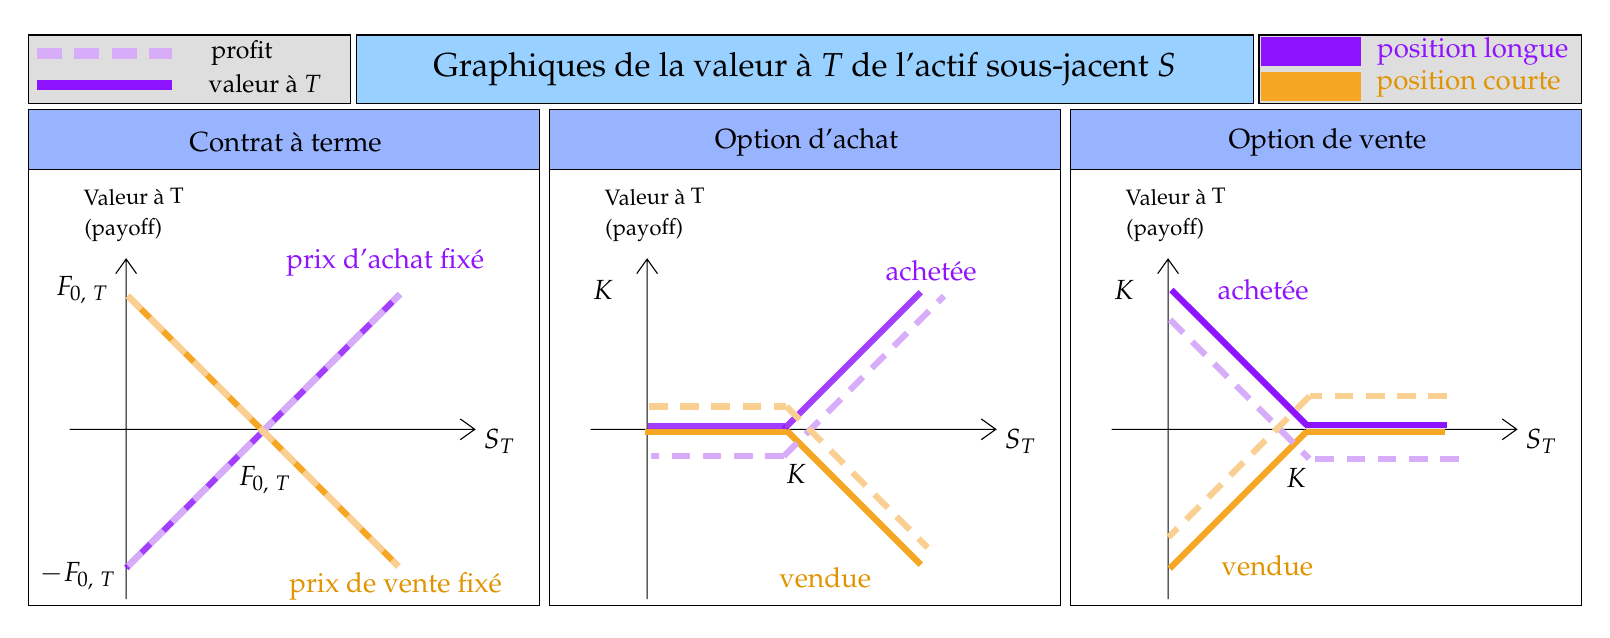
\begin{tikzpicture}[x=0.75pt,y=0.75pt,yscale=-1,xscale=1]
%uncomment if require: \path (0,309); %set diagram left start at 0, and has height of 309

%Shape: Rectangle [id:dp5014293673202075] 
\draw  [fill={rgb, 255:red, 152; green, 209; blue, 255 }  ,fill opacity=1 ] (185.17,2.33) -- (617.17,2.33) -- (617.17,35.33) -- (185.17,35.33) -- cycle ;
%Shape: Axis 2D [id:dp8910353553161174] 
\draw  (47,192.33) -- (242.17,192.33)(74.17,110.33) -- (74.17,274.17) (235.17,187.33) -- (242.17,192.33) -- (235.17,197.33) (69.17,117.33) -- (74.17,110.33) -- (79.17,117.33)  ;
%Straight Lines [id:da07902046514743155] 
\draw [color={rgb, 255:red, 245; green, 166; blue, 35 }  ,draw opacity=1 ][line width=2.25]    (75,128) -- (205.33,258.33) ;


%Straight Lines [id:da7529942024921858] 
\draw [color={rgb, 255:red, 142; green, 19; blue, 254 }  ,draw opacity=0.82 ][line width=2.25]    (74.25,259.08) -- (206.08,127.25) ;


%Shape: Rectangle [id:dp9569124985710353] 
\draw   (27,38.33) -- (273.17,38.33) -- (273.17,277.33) -- (27,277.33) -- cycle ;
%Shape: Rectangle [id:dp6038932286281922] 
\draw  [fill={rgb, 255:red, 152; green, 180; blue, 255 }  ,fill opacity=1 ] (27,38.33) -- (273.17,38.33) -- (273.17,67.13) -- (27,67.13) -- cycle ;
%Shape: Axis 2D [id:dp8487614270775223] 
\draw  (298,192.33) -- (493.17,192.33)(325.17,110.33) -- (325.17,274.17) (486.17,187.33) -- (493.17,192.33) -- (486.17,197.33) (320.17,117.33) -- (325.17,110.33) -- (330.17,117.33)  ;
%Straight Lines [id:da663442618971704] 
\draw [color={rgb, 255:red, 245; green, 166; blue, 35 }  ,draw opacity=1 ][line width=2.25]    (391.83,192.33) -- (457,257.5) ;


%Straight Lines [id:da8894317835492456] 
\draw [color={rgb, 255:red, 142; green, 19; blue, 254 }  ,draw opacity=0.82 ][line width=2.25]    (391,192.33) -- (457.08,126.25) ;


%Shape: Rectangle [id:dp8705141044857434] 
\draw   (278,38.33) -- (524.17,38.33) -- (524.17,277.33) -- (278,277.33) -- cycle ;
%Shape: Rectangle [id:dp12563706806770858] 
\draw  [fill={rgb, 255:red, 152; green, 180; blue, 255 }  ,fill opacity=1 ] (278,38.33) -- (524.17,38.33) -- (524.17,67.13) -- (278,67.13) -- cycle ;
%Straight Lines [id:da7370574620781261] 
\draw [color={rgb, 255:red, 142; green, 19; blue, 254 }  ,draw opacity=0.82 ][line width=2.25]    (325.54,190.62) -- (391.67,190.62) ;


%Straight Lines [id:da46421889356503176] 
\draw [color={rgb, 255:red, 245; green, 166; blue, 35 }  ,draw opacity=1 ][line width=2.25]    (324,193.62) -- (392.67,193.62) ;


%Shape: Axis 2D [id:dp12218006106251589] 
\draw  (549,192.33) -- (744.17,192.33)(576.17,110.33) -- (576.17,274.17) (737.17,187.33) -- (744.17,192.33) -- (737.17,197.33) (571.17,117.33) -- (576.17,110.33) -- (581.17,117.33)  ;
%Straight Lines [id:da05808191016293862] 
\draw [color={rgb, 255:red, 142; green, 19; blue, 254 }  ,draw opacity=1 ][line width=2.25]    (577.83,125.17) -- (643,190.33) ;


%Straight Lines [id:da6579640777364959] 
\draw [color={rgb, 255:red, 245; green, 166; blue, 35 }  ,draw opacity=1 ][line width=2.25]    (576.92,259.42) -- (643,193.33) ;


%Shape: Rectangle [id:dp6536765107760714] 
\draw   (529,38.33) -- (775.17,38.33) -- (775.17,277.33) -- (529,277.33) -- cycle ;
%Shape: Rectangle [id:dp8746319789223336] 
\draw  [fill={rgb, 255:red, 152; green, 180; blue, 255 }  ,fill opacity=1 ] (529,38.33) -- (775.17,38.33) -- (775.17,67.13) -- (529,67.13) -- cycle ;
%Straight Lines [id:da9314658151780497] 
\draw [color={rgb, 255:red, 245; green, 166; blue, 35 }  ,draw opacity=1 ][line width=2.25]    (709.67,193.62) -- (642.67,193.62) ;


%Straight Lines [id:da7353378001942827] 
\draw [color={rgb, 255:red, 142; green, 19; blue, 254 }  ,draw opacity=1 ][line width=2.25]    (642,190.33) -- (710.67,190.33) ;


%Straight Lines [id:da6447135481537327] 
\draw [color={rgb, 255:red, 215; green, 172; blue, 249 }  ,draw opacity=1 ][line width=2.25]  [dash pattern={on 6.75pt off 4.5pt}]  (75.17,258.17) -- (206.08,127.25) ;


%Straight Lines [id:da24025984300874126] 
\draw [color={rgb, 255:red, 215; green, 172; blue, 249 }  ,draw opacity=1 ][line width=2.25]  [dash pattern={on 6.75pt off 4.5pt}]  (391,205.33) -- (468.17,128.17) ;


%Straight Lines [id:da8831860343653457] 
\draw [color={rgb, 255:red, 215; green, 172; blue, 249 }  ,draw opacity=1 ][line width=2.25]  [dash pattern={on 6.75pt off 4.5pt}]  (391,205.33) -- (327.17,205.33) ;


%Straight Lines [id:da18639838701307276] 
\draw [color={rgb, 255:red, 215; green, 172; blue, 249 }  ,draw opacity=1 ][line width=2.25]  [dash pattern={on 6.75pt off 4.5pt}]  (577.17,139.5) -- (644.17,206.5) ;


%Straight Lines [id:da7126780450899792] 
\draw [color={rgb, 255:red, 215; green, 172; blue, 249 }  ,draw opacity=1 ][line width=2.25]  [dash pattern={on 6.75pt off 4.5pt}]  (716.17,206.5) -- (644.17,206.5) ;


%Straight Lines [id:da4974018498235153] 
\draw [color={rgb, 255:red, 249; green, 208; blue, 145 }  ,draw opacity=1 ][line width=2.25]  [dash pattern={on 6.75pt off 4.5pt}]  (75,128) -- (205.33,258.33) ;


%Straight Lines [id:da079381899397444] 
\draw [color={rgb, 255:red, 249; green, 208; blue, 145 }  ,draw opacity=1 ][line width=2.25]  [dash pattern={on 6.75pt off 4.5pt}]  (392.33,181.33) -- (460.33,249.33) ;


%Straight Lines [id:da6931960986042278] 
\draw [color={rgb, 255:red, 249; green, 208; blue, 145 }  ,draw opacity=1 ][line width=2.25]  [dash pattern={on 6.75pt off 4.5pt}]  (326.17,181.33) -- (392.33,181.33) ;


%Straight Lines [id:da13892219800463912] 
\draw [color={rgb, 255:red, 249; green, 208; blue, 145 }  ,draw opacity=1 ][line width=2.25]  [dash pattern={on 6.75pt off 4.5pt}]  (644.33,176.33) -- (576.33,244.33) ;


%Straight Lines [id:da8423794637164237] 
\draw [color={rgb, 255:red, 249; green, 208; blue, 145 }  ,draw opacity=1 ][line width=2.25]  [dash pattern={on 6.75pt off 4.5pt}]  (710.5,176.33) -- (644.33,176.33) ;


%Shape: Rectangle [id:dp6320359207595536] 
\draw  [fill={rgb, 255:red, 222; green, 222; blue, 222 }  ,fill opacity=1 ] (27,2.33) -- (182.17,2.33) -- (182.17,35.33) -- (27,35.33) -- cycle ;
%Straight Lines [id:da6914853181961316] 
\draw [color={rgb, 255:red, 215; green, 172; blue, 249 }  ,draw opacity=1 ][line width=3.75]  [dash pattern={on 9pt off 4.5pt}]  (31.17,11.33) -- (96.17,11.33) ;


%Straight Lines [id:da1620707780626105] 
\draw [color={rgb, 255:red, 142; green, 19; blue, 254 }  ,draw opacity=1 ][line width=3.75]    (31.17,26.33) -- (96.17,26.33) ;



%Shape: Rectangle [id:dp6695691986882595] 
\draw  [fill={rgb, 255:red, 222; green, 222; blue, 222 }  ,fill opacity=1 ] (620,2.33) -- (775.17,2.33) -- (775.17,35.33) -- (620,35.33) -- cycle ;
%Shape: Rectangle [id:dp31056838616590854] 
\draw  [draw opacity=0][fill={rgb, 255:red, 142; green, 19; blue, 254 }  ,fill opacity=1 ] (621,3.33) -- (669.17,3.33) -- (669.17,17.33) -- (621,17.33) -- cycle ;
%Shape: Rectangle [id:dp9578784787418022] 
\draw  [draw opacity=0][fill={rgb, 255:red, 245; green, 166; blue, 35 }  ,fill opacity=1 ] (621,20.33) -- (669.17,20.33) -- (669.17,34.33) -- (621,34.33) -- cycle ;


% Text Node
\draw (254,198) node   [align=left] {$\displaystyle S_{T}$};
% Text Node
\draw (53,125) node   [align=left] {$\displaystyle F_{0,\ T}$};
% Text Node
\draw (51,263) node   [align=left] {$\displaystyle -F_{0,\ T}$};
% Text Node
\draw (78,89) node  [font=\small,rotate=-358.99] [align=left] {{\footnotesize Valeur à T }\\{\footnotesize (payoff)}};
% Text Node
\draw (141,217) node   [align=left] {$\displaystyle F_{0,\ T}$};
% Text Node
\draw (151,54) node   [align=left] {Contrat à terme};
% Text Node
\draw (505,198) node   [align=left] {$\displaystyle S_{T}$};
% Text Node
\draw (304,125) node   [align=left] {$\displaystyle K$};
% Text Node
\draw (329,89) node  [font=\small,rotate=-358.99] [align=left] {{\footnotesize Valeur à T }\\{\footnotesize (payoff)}};
% Text Node
\draw (397,214) node   [align=left] {$\displaystyle K$};
% Text Node
\draw (401.17,18.83) node  [font=\large] [align=left] {Graphiques de la valeur à $\displaystyle T$ de l'actif sous-jacent $\displaystyle S$};
% Text Node
\draw (402,54) node   [align=left] {Option d'achat};
% Text Node
\draw (756,198) node   [align=left] {$\displaystyle S_{T}$};
% Text Node
\draw (555,125) node   [align=left] {$\displaystyle K$};
% Text Node
\draw (580,89) node  [font=\small,rotate=-358.99] [align=left] {{\footnotesize Valeur à T }\\{\footnotesize (payoff)}};
% Text Node
\draw (638,216) node   [align=left] {$\displaystyle K$};
% Text Node
\draw (653,54) node   [align=left] {Option de vente};
% Text Node
\draw (411,264) node  [color={rgb, 255:red, 225; green, 147; blue, 0 }  ,opacity=1 ] [align=left] {vendue};
% Text Node
\draw (204,268) node  [color={rgb, 255:red, 225; green, 147; blue, 0 }  ,opacity=1 ] [align=left] {prix de vente fixé};
% Text Node
\draw (462,116) node  [color={rgb, 255:red, 144; green, 19; blue, 254 }  ,opacity=1 ] [align=left] {achetée};
% Text Node
\draw (199,112) node  [color={rgb, 255:red, 144; green, 19; blue, 254 }  ,opacity=1 ] [align=left] {prix d'achat fixé};
% Text Node
\draw (130,11) node  [font=\small] [align=left] {profit};
% Text Node
\draw (141,26) node  [font=\small] [align=left] {valeur à $\displaystyle T$};
% Text Node
\draw (723,10) node  [color={rgb, 255:red, 144; green, 19; blue, 254 }  ,opacity=1 ] [align=left] {position longue};
% Text Node
\draw (721,26) node  [color={rgb, 255:red, 225; green, 147; blue, 0 }  ,opacity=1 ] [align=left] {position courte};
% Text Node
\draw (622,125) node  [color={rgb, 255:red, 144; green, 19; blue, 254 }  ,opacity=1 ] [align=left] {achetée};
% Text Node
\draw (624,258) node  [color={rgb, 255:red, 225; green, 147; blue, 0 }  ,opacity=1 ] [align=left] {vendue};


\end{tikzpicture}

\end{center}
\begin{center}
\begin{tabular}{|l	c	c	c|}
\hline
\rowcolor{blue(matcha)}
	Degré de parité	&	\og	\textit{Moneyness} \fg{}	&	Option d'achat	&	Option de vente	\\\hline
	au cours			&	\og	\textit{At-the-money} \fg{}		&	$S_{0} = K$	&	$S_{0} = K$	\\
	dans le cours	&	\og	\textit{In-the-money} \fg{} 	&	$S_{0} > K$	&	$S_{0} < K$	\\
	hors du cours	&	\og	\textit{Out-of-the-money} \fg{}	&	$S_{0} < K$	&	$S_{0} > K$	\\\specialrule{.10em}{.0em}{0.5em} 
\end{tabular}
\end{center}

\newpage
\begin{multicols*}{2}

\newpage

\section{Stratégies de couverture}
\subsection{Préliminaire}

\begin{conceptgen}{Hypothèses}
Pour tout le chapitre, nous posons les hypothèses suivantes:
\begin{multicols*}{2}
\begin{enumerate}[leftmargin = *]
	\item	Taux d'intérêt $i$ constant;
	\item	Aucuns frais de transaction;
	\item	Aucun risque de défaut;
	\item	Aucun versement intermédiaire.
\end{enumerate}
\end{multicols*}
\end{conceptgen}

\begin{rappel}{Propriétés des maximums et minimums}
\begin{align*}
	\max(a, b) + c	&=	\max(a + c, b + c)	\\
	\min(a, b) + c	&=	\min(a + c, b + c)	\\
	\min(a, b)	&=	-\max(-a, -b)	\\
	\max(a, b) \times c	&=	\max(a \times c, b \times c), \, c > 0	\\	
	\max(a, b) + \min(a, b)	&=	a + b	
\end{align*}
\end{rappel}

Une option est dite d'être non-couverte si nous avons aucune position dans l'actif sous-jacent. En revanche, une option est couverte si l'on a une position correspondant à l'obligation de l'option.	

Une \textbf{option d'achat couverte} est la \textbf{vente de l'option d'achat} $-C(K)$ et \textbf{l'achat du sous-jacent} $+S_{0}$.\\
Une \textbf{option de vente couverte} est la \textbf{vente de l'option de vente} $-P(K)$ et de \textbf{la vente à découvert du sous-jacent}.

\begin{definitionNOHFILL}[\textbf{Plancher} \og \textit{floor} \fg{}]
On achète une option de vente pour garantir un prix minimum de vente et couvrir une position longue dans l'actif sous-jacent. On dit donc avoir une \textbf{option de vente de protection} qui sert de \textit{plancher} minimale. 

\begin{align*}
	\text{Floor} 
	&=	+ S_{T} + P(K)	\\
	\text{Valeur à l'échéance} 
	&=	\max(0, K - S_{T}) + S_{T}
	=	\max(S_{T}, K)
\end{align*}
	
\begin{center}
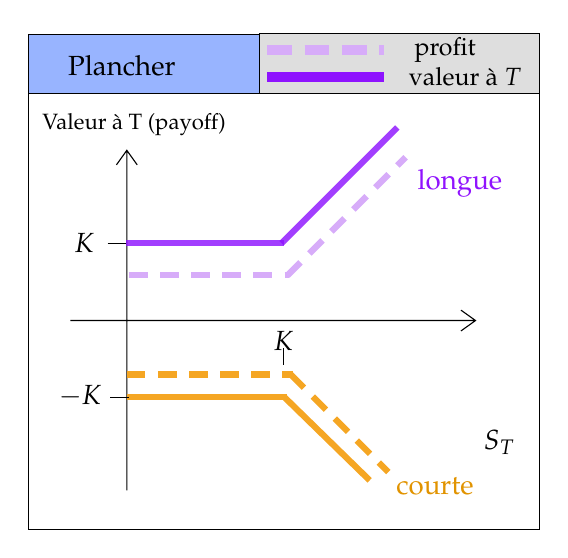
\begin{tikzpicture}[x=0.75pt,y=0.75pt,yscale=-1,xscale=1]
%uncomment if require: \path (0,281); %set diagram left start at 0, and has height of 281

%Shape: Axis 2D [id:dp40741511962973553] 
\draw  (49.33,155.67) -- (244.5,155.67)(76.5,73.67) -- (76.5,237.5) (237.5,150.67) -- (244.5,155.67) -- (237.5,160.67) (71.5,80.67) -- (76.5,73.67) -- (81.5,80.67)  ;
%Straight Lines [id:da9613660322224091] 
\draw [color={rgb, 255:red, 245; green, 166; blue, 35 }  ,draw opacity=1 ][line width=2.25]    (76.5,192.67) -- (153.5,192.67) ;
%Straight Lines [id:da5083823336560285] 
\draw [color={rgb, 255:red, 142; green, 19; blue, 254 }  ,draw opacity=0.82 ][line width=2.25]    (76.25,118.42) -- (152.08,118.42) ;
%Shape: Rectangle [id:dp6444257277769494] 
\draw   (29,17.67) -- (275.17,17.67) -- (275.17,256.33) -- (29,256.33) -- cycle ;
%Shape: Rectangle [id:dp1399374031728855] 
\draw  [fill={rgb, 255:red, 152; green, 180; blue, 255 }  ,fill opacity=1 ] (29,17.67) -- (275.17,17.67) -- (275.17,46.46) -- (29,46.46) -- cycle ;
%Straight Lines [id:da2304607321655061] 
\draw [color={rgb, 255:red, 215; green, 172; blue, 249 }  ,draw opacity=1 ][line width=2.25]  [dash pattern={on 6.75pt off 4.5pt}]  (77.5,133.67) -- (154.83,133.67) ;
%Shape: Rectangle [id:dp7590063931956115] 
\draw  [fill={rgb, 255:red, 222; green, 222; blue, 222 }  ,fill opacity=1 ] (140.54,17.56) -- (275.17,17.56) -- (275.17,46.19) -- (140.54,46.19) -- cycle ;
%Straight Lines [id:da9361199709983037] 
\draw [color={rgb, 255:red, 215; green, 172; blue, 249 }  ,draw opacity=1 ][line width=3.75]  [dash pattern={on 9pt off 4.5pt}]  (144.15,25.37) -- (200.55,25.37) ;
%Straight Lines [id:da5249384248345119] 
\draw [color={rgb, 255:red, 142; green, 19; blue, 254 }  ,draw opacity=1 ][line width=3.75]    (144.15,38.38) -- (200.55,38.38) ;

%Straight Lines [id:da5950286225671442] 
\draw    (67.25,118.42) -- (76.25,118.42) ;
%Straight Lines [id:da6670116946117266] 
\draw    (68.5,192.67) -- (77.5,192.67) ;
%Straight Lines [id:da3512128261940013] 
\draw    (151.83,177) -- (151.83,169) ;
%Straight Lines [id:da458962199402404] 
\draw [color={rgb, 255:red, 142; green, 19; blue, 254 }  ,draw opacity=0.82 ][line width=2.25]    (151.08,118.42) -- (206.83,62.67) ;
%Straight Lines [id:da3919562367284233] 
\draw [color={rgb, 255:red, 215; green, 172; blue, 249 }  ,draw opacity=1 ][line width=2.25]  [dash pattern={on 6.75pt off 4.5pt}]  (153.83,134) -- (210.83,77) ;
%Straight Lines [id:da2876164169742228] 
\draw [color={rgb, 255:red, 245; green, 166; blue, 35 }  ,draw opacity=1 ][line width=2.25]    (152.5,192.67) -- (193.5,232.67) ;
%Straight Lines [id:da8853700263616922] 
\draw [color={rgb, 255:red, 245; green, 166; blue, 35 }  ,draw opacity=1 ][line width=2.25]  [dash pattern={on 6.75pt off 4.5pt}]  (76.5,181.67) -- (156.5,181.67) ;
%Straight Lines [id:da1951691624983749] 
\draw [color={rgb, 255:red, 245; green, 166; blue, 35 }  ,draw opacity=1 ][line width=2.25]  [dash pattern={on 6.75pt off 4.5pt}]  (155.5,181.67) -- (202.5,228.67) ;

% Text Node
\draw (256,214.33) node   [align=left] {$\displaystyle S_{T}$};
% Text Node
\draw (56,118.33) node   [align=left] {$\displaystyle K$};
% Text Node
\draw (54,192.33) node   [align=left] {$\displaystyle -K$};
% Text Node
\draw (80,61.33) node  [font=\small] [align=left] {{\footnotesize Valeur à T (payoff)}};
% Text Node
\draw (74.08,33.06) node   [align=left] {Plancher};
% Text Node
\draw (225,235.33) node  [color={rgb, 255:red, 225; green, 147; blue, 0 }  ,opacity=1 ] [align=left] {courte};
% Text Node
\draw (237,89.33) node  [color={rgb, 255:red, 144; green, 19; blue, 254 }  ,opacity=1 ] [align=left] {longue};
% Text Node
\draw (239.45,38.09) node  [font=\small] [align=left] {valeur à $\displaystyle T$};
% Text Node
\draw (229.9,25.08) node  [font=\small] [align=left] {profit};
% Text Node
\draw (152,165.33) node   [align=left] {$\displaystyle K$};


\end{tikzpicture}
\end{center}
\end{definitionNOHFILL}

\begin{definitionNOHFILL}[\textbf{Plafond} \og \textit{cap} \fg{}]
On achète une option d'achat pour garantir un prix maximal d'achat et couvrir une position courte dans l'actif sous-jacent. Ce faisant, on \textit{plafonne} le prix d'achat.

\begin{align*}
	\text{Cap} 
	&=	- S_{T} + C(K)	\\
	\text{Valeur à l'échéance} 
	&=	\max(0, S_{T} - K) - S_{T}
	=	-\min(S_{T}, K)
\end{align*}

\begin{center}
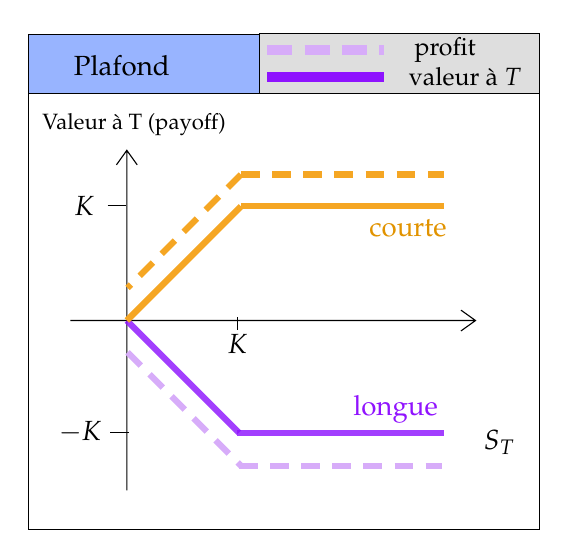
\begin{tikzpicture}[x=0.75pt,y=0.75pt,yscale=-1,xscale=1]
%uncomment if require: \path (0,281); %set diagram left start at 0, and has height of 281

%Shape: Axis 2D [id:dp7757310645686195] 
\draw  (309.33,155.67) -- (504.5,155.67)(336.5,73.67) -- (336.5,237.5) (497.5,150.67) -- (504.5,155.67) -- (497.5,160.67) (331.5,80.67) -- (336.5,73.67) -- (341.5,80.67)  ;
%Straight Lines [id:da44140392581623944] 
\draw [color={rgb, 255:red, 142; green, 19; blue, 254 }  ,draw opacity=0.82 ][line width=2.25]    (389.5,209.67) -- (489.5,209.67) ;
%Shape: Rectangle [id:dp4789469004418696] 
\draw   (289,17.67) -- (535.17,17.67) -- (535.17,256.33) -- (289,256.33) -- cycle ;
%Shape: Rectangle [id:dp5509836112302986] 
\draw  [fill={rgb, 255:red, 152; green, 180; blue, 255 }  ,fill opacity=1 ] (289,17.67) -- (535.17,17.67) -- (535.17,46.46) -- (289,46.46) -- cycle ;
%Straight Lines [id:da7062968329385482] 
\draw [color={rgb, 255:red, 215; green, 172; blue, 249 }  ,draw opacity=1 ][line width=2.25]  [dash pattern={on 6.75pt off 4.5pt}]  (390.5,225.67) -- (488.5,225.67) ;
%Shape: Rectangle [id:dp5326796083419292] 
\draw  [fill={rgb, 255:red, 222; green, 222; blue, 222 }  ,fill opacity=1 ] (400.54,17.56) -- (535.17,17.56) -- (535.17,46.19) -- (400.54,46.19) -- cycle ;
%Straight Lines [id:da06603476807124475] 
\draw [color={rgb, 255:red, 215; green, 172; blue, 249 }  ,draw opacity=1 ][line width=3.75]  [dash pattern={on 9pt off 4.5pt}]  (404.15,25.37) -- (460.55,25.37) ;
%Straight Lines [id:da9607284577943445] 
\draw [color={rgb, 255:red, 142; green, 19; blue, 254 }  ,draw opacity=1 ][line width=3.75]    (404.15,38.38) -- (460.55,38.38) ;

%Straight Lines [id:da41430412613503065] 
\draw    (327.25,100.42) -- (336.25,100.42) ;
%Straight Lines [id:da6138454710383172] 
\draw    (328.5,209.67) -- (337.5,209.67) ;
%Straight Lines [id:da45339912326496834] 
\draw    (389.83,160) -- (389.83,154) ;
%Straight Lines [id:da0570396071695729] 
\draw [color={rgb, 255:red, 142; green, 19; blue, 254 }  ,draw opacity=0.82 ][line width=2.25]    (336.5,155.67) -- (390.5,209.67) ;
%Straight Lines [id:da6083292817649542] 
\draw [color={rgb, 255:red, 215; green, 172; blue, 249 }  ,draw opacity=1 ][line width=2.25]  [dash pattern={on 6.75pt off 4.5pt}]  (336.83,171) -- (391.5,225.67) ;
%Straight Lines [id:da8504770158793074] 
\draw [color={rgb, 255:red, 245; green, 166; blue, 35 }  ,draw opacity=1 ][line width=2.25]    (391.5,100.67) -- (336.5,155.67) ;
%Straight Lines [id:da08352414862449642] 
\draw [color={rgb, 255:red, 245; green, 166; blue, 35 }  ,draw opacity=1 ][line width=2.25]    (391.5,100.67) -- (489.5,100.67) ;
%Straight Lines [id:da2274948316125296] 
\draw [color={rgb, 255:red, 245; green, 166; blue, 35 }  ,draw opacity=1 ][line width=2.25]  [dash pattern={on 6.75pt off 4.5pt}]  (391.5,85.33) -- (336.83,140) ;
%Straight Lines [id:da021196981051522013] 
\draw [color={rgb, 255:red, 245; green, 166; blue, 35 }  ,draw opacity=1 ][line width=2.25]  [dash pattern={on 6.75pt off 4.5pt}]  (391.5,85.33) -- (489.5,85.33) ;

% Text Node
\draw (516,214.33) node   [align=left] {$\displaystyle S_{T}$};
% Text Node
\draw (316,100.33) node   [align=left] {$\displaystyle K$};
% Text Node
\draw (314,209.33) node   [align=left] {$\displaystyle -K$};
% Text Node
\draw (340,61.33) node  [font=\small] [align=left] {{\footnotesize Valeur à T (payoff)}};
% Text Node
\draw (334.08,33.06) node   [align=left] {Plafond};
% Text Node
\draw (466,198.33) node  [color={rgb, 255:red, 144; green, 19; blue, 254 }  ,opacity=1 ] [align=left] {longue};
% Text Node
\draw (389.83,167) node   [align=left] {$\displaystyle K$};
% Text Node
\draw (499.45,38.09) node  [font=\small] [align=left] {valeur à $\displaystyle T$};
% Text Node
\draw (489.9,25.08) node  [font=\small] [align=left] {profit};
% Text Node
\draw (472,111.33) node  [color={rgb, 255:red, 225; green, 147; blue, 0 }  ,opacity=1 ] [align=left] {courte};


\end{tikzpicture}
\end{center}
\end{definitionNOHFILL}

\columnbreak

\subsection{Écarts et tunnels}

\begin{definitionNOHFILL}[\textbf{Écart haussier} \og \textit{Bull Spread} \fg{}]
Crée en:
\begin{itemize}[leftmargin = *]
	\item	Achetant une option d'achat $C(K_{1})$ et vendant une autre option achat $C(K_{2})$  à un prix d'exercice plus élevé $K_{2} > K_{1}$;
	\item	Achetant une option de vente $P(K_{1})$ et vendant une autre option de vente $P(K_{2})$ à un prix d'exercice plus élevé $K_{2} > K_{1}$.
\end{itemize}

\begin{distributions}[Contexte]
\begin{itemize}[leftmargin = *]
	\item	Typiquement utilisé lorsqu'un investisseur croit que, entre deux prix d'exercice, le prix va augmenter, \textit{\textbf{mais}}
		\begin{itemize}[leftmargin = *]
		\item	Qu'il ne veut pas une perte trop importante si le prix de l'actif baisse;
		\item	Ni qu'il veut payer pour plus de profit qu'il s'attend à recevoir.
		\end{itemize}
	\item	\og \textit{Bull Spread} \fg{} provient de l'idée d'être \og \textit{\textbf{bull}-ish} \fg{} et prévoir une augmentation du prix de l'action à un intervalle;
	\item[]	On peut également visualiser un taureau avec ses cornes pointues vers le haut prêt à attaquer.
\end{itemize}
\end{distributions}

\begin{center}
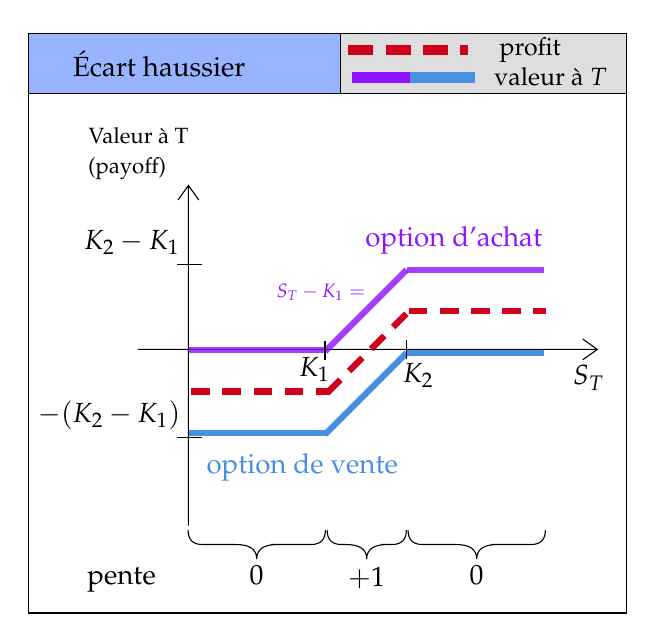
\begin{tikzpicture}[x=0.75pt,y=0.75pt,yscale=-1,xscale=1]
%uncomment if require: \path (0,349.33333587646484); %set diagram left start at 0, and has height of 349.33333587646484

%Shape: Axis 2D [id:dp7601418140814886] 
\draw  (80,190.33) -- (301.17,190.33)(104.17,111.33) -- (104.17,275.17) (294.17,185.33) -- (301.17,190.33) -- (294.17,195.33) (99.17,118.33) -- (104.17,111.33) -- (109.17,118.33)  ;
%Straight Lines [id:da41700930229104993] 
\draw [color={rgb, 255:red, 142; green, 19; blue, 254 }  ,draw opacity=0.82 ][line width=2.25]    (170,191.33) -- (209.33,152) ;


%Shape: Rectangle [id:dp3515130332085854] 
\draw   (27,38.33) -- (315.17,38.33) -- (315.17,317.33) -- (27,317.33) -- cycle ;
%Shape: Rectangle [id:dp13591016175410142] 
\draw  [fill={rgb, 255:red, 152; green, 180; blue, 255 }  ,fill opacity=1 ] (27,38.33) -- (315.17,38.33) -- (315.17,67.13) -- (27,67.13) -- cycle ;
%Straight Lines [id:da8110867387524421] 
\draw [color={rgb, 255:red, 142; green, 19; blue, 254 }  ,draw opacity=0.82 ][line width=2.25]    (104.54,190.62) -- (170.67,190.62) ;


%Shape: Rectangle [id:dp6374879389517476] 
\draw  [fill={rgb, 255:red, 222; green, 222; blue, 222 }  ,fill opacity=1 ] (177.5,38.24) -- (315.17,38.24) -- (315.17,67.09) -- (177.5,67.09) -- cycle ;
%Straight Lines [id:da38766311196421266] 
\draw [color={rgb, 255:red, 208; green, 2; blue, 27 }  ,draw opacity=1 ][line width=3.75]  [dash pattern={on 9pt off 4.5pt}]  (181.2,46.11) -- (238.87,46.11) ;


%Straight Lines [id:da8251624196749612] 
\draw [color={rgb, 255:red, 142; green, 19; blue, 254 }  ,draw opacity=1 ][line width=3.75]    (183.17,59.33) -- (211.17,59.33) ;


%Straight Lines [id:da7333005166945665] 
\draw [color={rgb, 255:red, 142; green, 19; blue, 254 }  ,draw opacity=0.82 ][line width=2.25]    (209.33,152) -- (275.46,152) ;


%Straight Lines [id:da7002889517266064] 
\draw [color={rgb, 255:red, 74; green, 144; blue, 226 }  ,draw opacity=1 ][line width=2.25]    (170,231.33) -- (209.33,192) ;


%Straight Lines [id:da9040823354436966] 
\draw [color={rgb, 255:red, 74; green, 144; blue, 226 }  ,draw opacity=1 ][line width=2.25]    (104.54,230.62) -- (170.67,230.62) ;


%Straight Lines [id:da5330320430279016] 
\draw [color={rgb, 255:red, 74; green, 144; blue, 226 }  ,draw opacity=1 ][line width=2.25]    (209.33,192) -- (275.46,192) ;


%Straight Lines [id:da4473231719641506] 
\draw    (98.83,149.33) -- (110.83,149.33) ;


%Straight Lines [id:da6014598987525124] 
\draw    (98.54,232.62) -- (110.54,232.62) ;


%Straight Lines [id:da5589803186094386] 
\draw [color={rgb, 255:red, 208; green, 2; blue, 27 }  ,draw opacity=1 ][line width=2.25]  [dash pattern={on 6.75pt off 4.5pt}]  (171,211.33) -- (210.33,172) ;


%Straight Lines [id:da9151952042747453] 
\draw [color={rgb, 255:red, 208; green, 2; blue, 27 }  ,draw opacity=1 ][line width=2.25]  [dash pattern={on 6.75pt off 4.5pt}]  (105.54,210.62) -- (171.67,210.62) ;


%Straight Lines [id:da26907052178753155] 
\draw [color={rgb, 255:red, 208; green, 2; blue, 27 }  ,draw opacity=1 ][line width=2.25]  [dash pattern={on 6.75pt off 4.5pt}]  (210.33,172) -- (276.46,172) ;


%Shape: Brace [id:dp25440966898606243] 
\draw   (104,277.33) .. controls (104,282) and (106.33,284.33) .. (111,284.33) -- (127.08,284.33) .. controls (133.75,284.33) and (137.08,286.66) .. (137.08,291.33) .. controls (137.08,286.66) and (140.41,284.33) .. (147.08,284.33)(144.08,284.33) -- (163.17,284.33) .. controls (167.84,284.33) and (170.17,282) .. (170.17,277.33) ;
%Shape: Brace [id:dp5464922629290294] 
\draw   (171,277.33) .. controls (171,282) and (173.33,284.33) .. (178,284.33) -- (180.08,284.33) .. controls (186.75,284.33) and (190.08,286.66) .. (190.08,291.33) .. controls (190.08,286.66) and (193.41,284.33) .. (200.08,284.33)(197.08,284.33) -- (202.17,284.33) .. controls (206.84,284.33) and (209.17,282) .. (209.17,277.33) ;
%Shape: Brace [id:dp8339351145442746] 
\draw   (210,277.33) .. controls (210,282) and (212.33,284.33) .. (217,284.33) -- (233.08,284.33) .. controls (239.75,284.33) and (243.08,286.66) .. (243.08,291.33) .. controls (243.08,286.66) and (246.41,284.33) .. (253.08,284.33)(250.08,284.33) -- (269.17,284.33) .. controls (273.84,284.33) and (276.17,282) .. (276.17,277.33) ;
%Straight Lines [id:da6494635826891548] 
\draw    (170,195.33) -- (170,186.33) ;


%Straight Lines [id:da9618527970027351] 
\draw    (209.33,195) -- (209.33,186) ;


%Straight Lines [id:da34278626539211876] 
\draw [color={rgb, 255:red, 74; green, 144; blue, 226 }  ,draw opacity=1 ][line width=3.75]    (211.17,59.33) -- (242.17,59.33) ;



% Text Node
\draw (297,204) node   [align=left] {$\displaystyle S_{T}$};
% Text Node
\draw (77,139) node   [align=left] {$\displaystyle K_{2} -K_{1}$};
% Text Node
\draw (80,96) node  [font=\small,rotate=-0.4] [align=left] {{\footnotesize Valeur à T }\\{\footnotesize (payoff)}};
% Text Node
\draw (165,200) node   [align=left] {$\displaystyle K_{1}$};
% Text Node
\draw (90.08,52.73) node   [align=left] {Écart haussier};
% Text Node
\draw (232,138) node  [color={rgb, 255:red, 144; green, 19; blue, 254 }  ,opacity=1 ] [align=left] {option d'achat};
% Text Node
\draw (215,203) node   [align=left] {$\displaystyle K_{2}$};
% Text Node
\draw (159,247) node  [color={rgb, 255:red, 144; green, 19; blue, 254 }  ,opacity=1 ] [align=left] {\textcolor[rgb]{0.29,0.56,0.89}{option de vente}};
% Text Node
\draw (66,222) node   [align=left] {$\displaystyle -( K_{2} -K_{1})$};
% Text Node
\draw (72,301.33) node   [align=left] {pente};
% Text Node
\draw (137,299.33) node   [align=left] {$\displaystyle 0$};
% Text Node
\draw (190,300.33) node   [align=left] {$\displaystyle +1$};
% Text Node
\draw (243,299.33) node   [align=left] {$\displaystyle 0$};
% Text Node
\draw (168,163) node  [font=\scriptsize,color={rgb, 255:red, 144; green, 19; blue, 254 }  ,opacity=1 ] [align=left] {$\displaystyle S_{T} -K_{1} =$};
% Text Node
\draw (268.88,45.82) node  [font=\small] [align=left] {profit};
% Text Node
\draw (278.64,58.93) node  [font=\small] [align=left] {valeur à $\displaystyle T$};

\end{tikzpicture}
\end{center}
\end{definitionNOHFILL}

\begin{definitionNOHFILL}[\textbf{Écart baissier} \og \textit{Bear Spread} \fg{}]
L'inverse d'un écart haussier, il est crée en:
\begin{itemize}[leftmargin = *]
	\item	Vendant une option d'achat $C(K_{1})$ et achetant une autre option achat $C(K_{2})$  à un prix d'exercice plus élevé $K_{2} > K_{1}$;
	\item	Vendant une option de vente $P(K_{1})$ et achetant une autre option de vente $P(K_{2})$ à un prix d'exercice plus élevé $K_{2} > K_{1}$.
\end{itemize}

\begin{distributions}[Contexte]
\begin{itemize}[leftmargin = *]
	\item	Typiquement utilisé lorsqu'un investisseur croit que, entre deux prix d'exercice, le prix va baisser, \textit{\textbf{mais}} qu'il
		\begin{itemize}[leftmargin = *]
		\item	Qu'il ne veut pas une perte trop importante si le prix de l'actif baisse;
		\item	Ni qu'il veut payer pour plus de profit qu'il s'attend à recevoir.
		\end{itemize}
	\item	\og \textit{Bear Spread} \fg{} provient de l'idée d'investir avec précaution pour \og \textit{\textbf{bear}-er} \fg{} une et baisse du prix de l'action à un intervalle;
	\item[]	On peut également visualiser un ours qui va \og strike down \fg{} avec ses pattes d'ours en attaque.
\end{itemize}
\end{distributions}


\begin{center}
\tikzset{every picture/.style={line width=0.75pt}} %set default line width to 0.75pt        
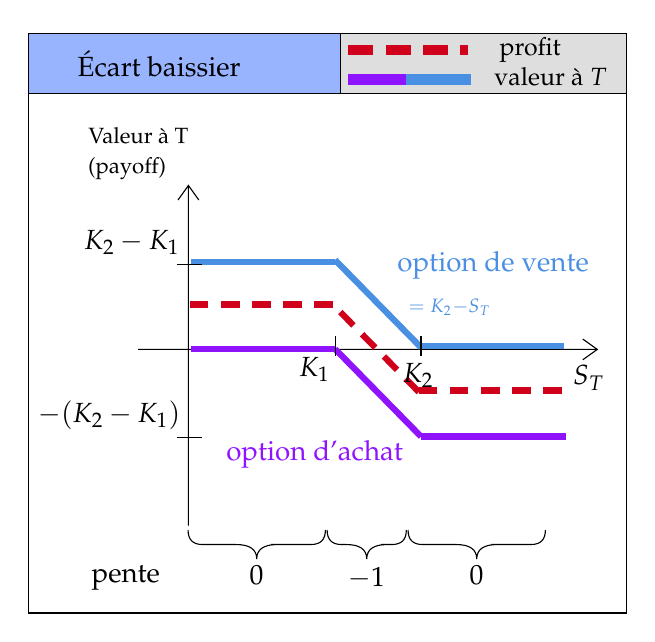
\begin{tikzpicture}[x=0.75pt,y=0.75pt,yscale=-1,xscale=1]
%uncomment if require: \path (0,349.33333587646484); %set diagram left start at 0, and has height of 349.33333587646484

%Shape: Axis 2D [id:dp680976564625396] 
\draw  (375,190.33) -- (596.17,190.33)(399.17,111.33) -- (399.17,275.17) (589.17,185.33) -- (596.17,190.33) -- (589.17,195.33) (394.17,118.33) -- (399.17,111.33) -- (404.17,118.33)  ;
%Straight Lines [id:da5848322385212859] 
\draw [color={rgb, 255:red, 74; green, 144; blue, 226 }  ,draw opacity=1 ][line width=2.25]    (511.25,189.41) -- (469.84,147.23) ;


%Shape: Rectangle [id:dp35378675230131185] 
\draw   (322,38.33) -- (610.17,38.33) -- (610.17,317.33) -- (322,317.33) -- cycle ;
%Shape: Rectangle [id:dp5176381224989448] 
\draw  [fill={rgb, 255:red, 152; green, 180; blue, 255 }  ,fill opacity=1 ] (322,38.33) -- (610.17,38.33) -- (610.17,67.13) -- (322,67.13) -- cycle ;
%Straight Lines [id:da16417371671750347] 
\draw [color={rgb, 255:red, 74; green, 144; blue, 226 }  ,draw opacity=1 ][line width=2.25]    (580.17,188.65) -- (510.55,188.65) ;


%Straight Lines [id:da3198620949992881] 
\draw [color={rgb, 255:red, 74; green, 144; blue, 226 }  ,draw opacity=1 ][line width=2.25]    (469.84,148.23) -- (400.22,148.23) ;


%Straight Lines [id:da5036887985940388] 
\draw [color={rgb, 255:red, 144; green, 19; blue, 254 }  ,draw opacity=1 ][line width=2.25]    (511.25,232.31) -- (469.84,190.13) ;


%Straight Lines [id:da3322721142838323] 
\draw [color={rgb, 255:red, 144; green, 19; blue, 254 }  ,draw opacity=1 ][line width=2.25]    (580.87,232.31) -- (511.25,232.31) ;


%Straight Lines [id:da8890931859596114] 
\draw [color={rgb, 255:red, 144; green, 19; blue, 254 }  ,draw opacity=1 ][line width=2.25]    (469.84,190.13) -- (400.22,190.13) ;


%Straight Lines [id:da07817633570689475] 
\draw    (393.83,149.33) -- (405.83,149.33) ;


%Straight Lines [id:da7851330337121041] 
\draw    (393.54,232.62) -- (405.54,232.62) ;


%Straight Lines [id:da7852978808587163] 
\draw [color={rgb, 255:red, 208; green, 2; blue, 27 }  ,draw opacity=1 ][line width=2.25]  [dash pattern={on 6.75pt off 4.5pt}]  (510.2,210.86) -- (468.79,168.68) ;


%Straight Lines [id:da7015379305827307] 
\draw [color={rgb, 255:red, 208; green, 2; blue, 27 }  ,draw opacity=1 ][line width=2.25]  [dash pattern={on 6.75pt off 4.5pt}]  (579.11,210.1) -- (509.5,210.1) ;


%Straight Lines [id:da47582543050744275] 
\draw [color={rgb, 255:red, 208; green, 2; blue, 27 }  ,draw opacity=1 ][line width=2.25]  [dash pattern={on 6.75pt off 4.5pt}]  (468.79,168.68) -- (399.17,168.68) ;


%Shape: Brace [id:dp1704100229687211] 
\draw   (399,277.33) .. controls (399,282) and (401.33,284.33) .. (406,284.33) -- (422.08,284.33) .. controls (428.75,284.33) and (432.08,286.66) .. (432.08,291.33) .. controls (432.08,286.66) and (435.41,284.33) .. (442.08,284.33)(439.08,284.33) -- (458.17,284.33) .. controls (462.84,284.33) and (465.17,282) .. (465.17,277.33) ;
%Shape: Brace [id:dp8688743767541778] 
\draw   (466,277.33) .. controls (466,282) and (468.33,284.33) .. (473,284.33) -- (475.08,284.33) .. controls (481.75,284.33) and (485.08,286.66) .. (485.08,291.33) .. controls (485.08,286.66) and (488.41,284.33) .. (495.08,284.33)(492.08,284.33) -- (497.17,284.33) .. controls (501.84,284.33) and (504.17,282) .. (504.17,277.33) ;
%Shape: Brace [id:dp5219365881869815] 
\draw   (505,277.33) .. controls (505,282) and (507.33,284.33) .. (512,284.33) -- (528.08,284.33) .. controls (534.75,284.33) and (538.08,286.66) .. (538.08,291.33) .. controls (538.08,286.66) and (541.41,284.33) .. (548.08,284.33)(545.08,284.33) -- (564.17,284.33) .. controls (568.84,284.33) and (571.17,282) .. (571.17,277.33) ;
%Straight Lines [id:da9076040627764943] 
\draw    (511.25,193.7) -- (511.25,184.05) ;


%Straight Lines [id:da17266836853894918] 
\draw    (469.84,193.35) -- (469.84,183.69) ;


%Shape: Rectangle [id:dp7827835139171508] 
\draw  [fill={rgb, 255:red, 222; green, 222; blue, 222 }  ,fill opacity=1 ] (472.5,38.24) -- (610.17,38.24) -- (610.17,67.09) -- (472.5,67.09) -- cycle ;
%Straight Lines [id:da899380327396603] 
\draw [color={rgb, 255:red, 208; green, 2; blue, 27 }  ,draw opacity=1 ][line width=3.75]  [dash pattern={on 9pt off 4.5pt}]  (476.2,46.11) -- (533.87,46.11) ;


%Straight Lines [id:da14625994420742927] 
\draw [color={rgb, 255:red, 142; green, 19; blue, 254 }  ,draw opacity=1 ][line width=3.75]    (476.17,60.33) -- (504.17,60.33) ;


%Straight Lines [id:da9746587617345248] 
\draw [color={rgb, 255:red, 74; green, 144; blue, 226 }  ,draw opacity=1 ][line width=3.75]    (504.17,60.33) -- (535.17,60.33) ;



% Text Node
\draw (592,204) node   [align=left] {$\displaystyle S_{T}$};
% Text Node
\draw (372,139) node   [align=left] {$\displaystyle K_{2} -K_{1}$};
% Text Node
\draw (375,96) node  [font=\small,rotate=-0.4] [align=left] {{\footnotesize Valeur à T }\\{\footnotesize (payoff)}};
% Text Node
\draw (460,200) node   [align=left] {$\displaystyle K_{1}$};
% Text Node
\draw (385.08,52.73) node   [align=left] {Écart baissier};
% Text Node
\draw (460,241) node  [color={rgb, 255:red, 144; green, 19; blue, 254 }  ,opacity=1 ] [align=left] {option d'achat};
% Text Node
\draw (510,203) node   [align=left] {$\displaystyle K_{2}$};
% Text Node
\draw (546,150) node  [color={rgb, 255:red, 144; green, 19; blue, 254 }  ,opacity=1 ] [align=left] {\textcolor[rgb]{0.29,0.56,0.89}{option de vente}};
% Text Node
\draw (361,222) node   [align=left] {$\displaystyle -( K_{2} -K_{1})$};
% Text Node
\draw (369,300.33) node   [align=left] {pente};
% Text Node
\draw (432,299.33) node   [align=left] {$\displaystyle 0$};
% Text Node
\draw (485,300.33) node   [align=left] {$\displaystyle -1$};
% Text Node
\draw (538,299.33) node   [align=left] {$\displaystyle 0$};
% Text Node
\draw (525,170) node  [font=\scriptsize,color={rgb, 255:red, 144; green, 19; blue, 254 }  ,opacity=1 ] [align=left] {$\displaystyle \textcolor[rgb]{0.29,0.56,0.89}{=K}\textcolor[rgb]{0.29,0.56,0.89}{_{2}}\textcolor[rgb]{0.29,0.56,0.89}{-S}\textcolor[rgb]{0.29,0.56,0.89}{_{T}}$};
% Text Node
\draw (573.64,58.93) node  [font=\small] [align=left] {valeur à $\displaystyle T$};
% Text Node
\draw (563.88,45.82) node  [font=\small] [align=left] {profit};


\end{tikzpicture}
\end{center}
	
\end{definitionNOHFILL}

\begin{definitionNOHFILL}[\textbf{Écart sur ratio d'options} \og \textit{Ratio Spread} \fg{}]
Crée en:
\begin{itemize}[leftmargin = *]
	\item	\textbf{achetant} $m$ options à un prix d'exercice $K_{1}$ et
	\item	puis \textbf{vendant} $n$ options à un prix d'exercice $K_{2}$ différent où
	\item	$m \neq n$ et $K_{1} \neq K_{2}$.
\end{itemize}

\end{definitionNOHFILL}

\begin{definitionNOHFILL}[\textbf{Boite} \og \textit{Box Spread} \fg{}]
\begin{itemize}[leftmargin = *]
	\item	La stratégie consiste à acheter un écart haussier ainsi qu'un écart baissier où l'un utilise des options d'achat et l'autre des options de vente (ayant les mêmes caractéristiques);
	\item	Il est utilisé pour emprunter ou prêter de l'argent avec une valeur à l'échéance connue en avance, peu importe la direction prise par la valeur de l'actif sous-jacent;
	\item	Il est donc équivalent à une obligation zéro-coupons.
\end{itemize}

\begin{center}
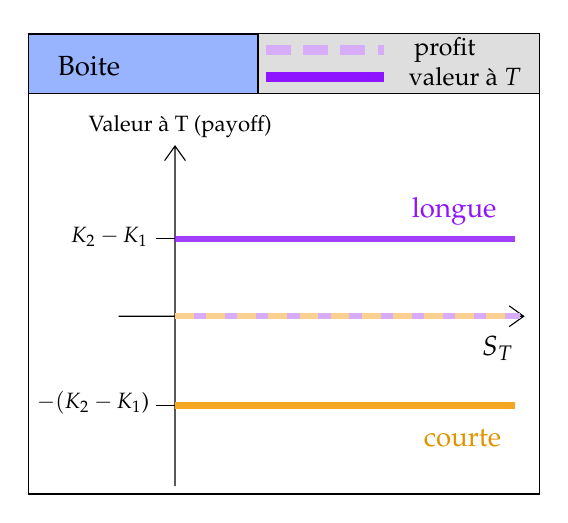
\begin{tikzpicture}[x=0.75pt,y=0.75pt,yscale=-1,xscale=1]
%uncomment if require: \path (0,300); %set diagram left start at 0, and has height of 300

%Shape: Axis 2D [id:dp3944596414442396] 
\draw  (91.33,187.33) -- (286.5,187.33)(118.5,105.33) -- (118.5,269.17) (279.5,182.33) -- (286.5,187.33) -- (279.5,192.33) (113.5,112.33) -- (118.5,105.33) -- (123.5,112.33)  ;
%Straight Lines [id:da9198165153485065] 
\draw [color={rgb, 255:red, 245; green, 166; blue, 35 }  ,draw opacity=1 ][line width=2.25]    (118.5,230.33) -- (282.5,230.33) ;
%Straight Lines [id:da2727787244780491] 
\draw [color={rgb, 255:red, 142; green, 19; blue, 254 }  ,draw opacity=0.82 ][line width=2.25]    (118.25,150.08) -- (282.5,150.08) ;
%Shape: Rectangle [id:dp979071417841511] 
\draw   (48,51.33) -- (294.17,51.33) -- (294.17,273) -- (48,273) -- cycle ;
%Shape: Rectangle [id:dp13997180603804438] 
\draw  [fill={rgb, 255:red, 152; green, 180; blue, 255 }  ,fill opacity=1 ] (48,51.33) -- (294.17,51.33) -- (294.17,80.13) -- (48,80.13) -- cycle ;
%Straight Lines [id:da6758956259405962] 
\draw [color={rgb, 255:red, 215; green, 172; blue, 249 }  ,draw opacity=1 ][line width=2.25]  [dash pattern={on 6.75pt off 4.5pt}]  (125.5,187.33) -- (285.5,187.33) ;
%Straight Lines [id:da43948542993181694] 
\draw [color={rgb, 255:red, 249; green, 208; blue, 145 }  ,draw opacity=1 ][line width=2.25]  [dash pattern={on 6.75pt off 4.5pt}]  (118.5,187.33) -- (283.33,187.33) ;
%Shape: Rectangle [id:dp13021060497393955] 
\draw  [fill={rgb, 255:red, 222; green, 222; blue, 222 }  ,fill opacity=1 ] (158.5,51.23) -- (294.17,51.23) -- (294.17,80.08) -- (158.5,80.08) -- cycle ;
%Straight Lines [id:da6465832507201692] 
\draw [color={rgb, 255:red, 215; green, 172; blue, 249 }  ,draw opacity=1 ][line width=3.75]  [dash pattern={on 9pt off 4.5pt}]  (162.14,59.1) -- (218.97,59.1) ;
%Straight Lines [id:da4781032794703184] 
\draw [color={rgb, 255:red, 142; green, 19; blue, 254 }  ,draw opacity=1 ][line width=3.75]    (162.14,72.21) -- (218.97,72.21) ;

%Straight Lines [id:da36665207085211926] 
\draw    (109.25,150.08) -- (118.25,150.08) ;
%Straight Lines [id:da33360724695448285] 
\draw    (109.5,230.33) -- (118.5,230.33) ;

% Text Node
\draw (274,203) node   [align=left] {$\displaystyle S_{T}$};
% Text Node
\draw (87,149) node  [font=\footnotesize] [align=left] {$\displaystyle K_{2} -K_{1}$};
% Text Node
\draw (121,96) node  [font=\small] [align=left] {{\footnotesize Valeur à T (payoff)}};
% Text Node
\draw (77.08,66.73) node   [align=left] {Boite};
% Text Node
\draw (257,246) node  [color={rgb, 255:red, 225; green, 147; blue, 0 }  ,opacity=1 ] [align=left] {courte};
% Text Node
\draw (253,137) node  [color={rgb, 255:red, 144; green, 19; blue, 254 }  ,opacity=1 ] [align=left] {longue};
% Text Node
\draw (258.17,71.92) node  [font=\small] [align=left] {valeur à $\displaystyle T$};
% Text Node
\draw (248.56,58.81) node  [font=\small] [align=left] {profit};
% Text Node
\draw (79,229) node  [font=\footnotesize] [align=left] {$\displaystyle -( K_{2} -K_{1}$)};


\end{tikzpicture}
\end{center}

Par exemple, on achète (position longue) un écart haussier d'options d'achat et un écart baisser d'options de vente:
\begin{center}
\begin{tabular}{|	c	|	c	|	c	|	c	|}
\hline
\rowcolor{blue(matcha)}
	\textbf{option}		&	$0 \le S_{T} < K_{1}$	&	$K_{1} \le S_{T} < K_{2}$	&	$K_{2} \le S_{T}$	\\\hline
	$+C(K_{1})$	&	$0$					&	$S_{T} - K_{1}$	&	$S_{T} - K_{1}$	\\
	$-C(K_{2})$	&	$0$					&	$0$				&	$-(S_{T} - K_{2})$	\\
	$-P(K_{1})$	&	$-(K_{1} - S_{T})$	&	$0$				&	$0$	\\
	$+P(K_{2})$	&	$K_{2} - S_{T}$		&	$K_{2} - S_{T}$	&	$0$	\\\specialrule{.10em}{.0em}{0.0em} 
	\textbf{net}	&	$K_{2} - K_{1}$	&	$K_{2} - K_{1}$	&	$K_{2} - K_{1}$	\\\specialrule{.10em}{.0em}{0.5em} 
\end{tabular}
\end{center}
\end{definitionNOHFILL}

\begin{definitionNOHFILL}[\textbf{Tunnel} \og \textit{Collar} \fg{} et \textbf{action couverte par un tunnel} \og \textit{Collared stock} \fg{} ]
Le tunnel (\og \textit{Collar} \fg{}) est crée en
\begin{itemize}[leftmargin = *]
	\item	Achetant une option de vente $P(K_{1})$ et 
	\item	vendant une option d'achat $C(K_{2})$ où
	\item	$K_{1} < K_{2}$.
\end{itemize}

Lorsqu'on achète l'actif (position longue) en plus, nous obtenons une action couverte par un tunnel (\og \textit{Collared stock} \fg{}).

La largeur du tunnel est $K_{2} - K_{1}$.

\begin{center}


\tikzset{every picture/.style={line width=0.75pt}} %set default line width to 0.75pt        

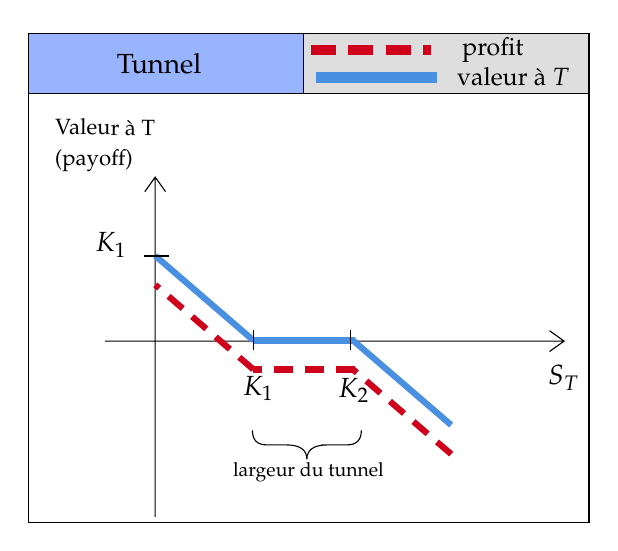
\begin{tikzpicture}[x=0.75pt,y=0.75pt,yscale=-1,xscale=1]
%uncomment if require: \path (0,349.33333587646484); %set diagram left start at 0, and has height of 349.33333587646484

%Shape: Rectangle [id:dp3515130332085854] 
\draw   (27,38.33) -- (297.17,38.33) -- (297.17,273.67) -- (27,273.67) -- cycle ;
%Shape: Rectangle [id:dp13591016175410142] 
\draw  [fill={rgb, 255:red, 152; green, 180; blue, 255 }  ,fill opacity=1 ] (27,38.33) -- (297.17,38.33) -- (297.17,67.13) -- (27,67.13) -- cycle ;
%Shape: Rectangle [id:dp6374879389517476] 
\draw  [fill={rgb, 255:red, 222; green, 222; blue, 222 }  ,fill opacity=1 ] (159.5,38.24) -- (297.17,38.24) -- (297.17,67.09) -- (159.5,67.09) -- cycle ;
%Straight Lines [id:da38766311196421266] 
\draw [color={rgb, 255:red, 208; green, 2; blue, 27 }  ,draw opacity=1 ][line width=3.75]  [dash pattern={on 9pt off 4.5pt}]  (163.2,46.11) -- (220.87,46.11) ;


%Straight Lines [id:da34278626539211876] 
\draw [color={rgb, 255:red, 74; green, 144; blue, 226 }  ,draw opacity=1 ][line width=3.75]    (165.5,59.33) -- (224.17,59.33) ;


%Shape: Axis 2D [id:dp9727644255367149] 
\draw  (64,186.33) -- (285.17,186.33)(88.17,107.33) -- (88.17,271.17) (278.17,181.33) -- (285.17,186.33) -- (278.17,191.33) (83.17,114.33) -- (88.17,107.33) -- (93.17,114.33)  ;
%Straight Lines [id:da6780443513094567] 
\draw [color={rgb, 255:red, 74; green, 144; blue, 226 }  ,draw opacity=1 ][line width=2.25]    (135.5,186) -- (88.22,145.23) ;


%Straight Lines [id:da5925572195913587] 
\draw [color={rgb, 255:red, 74; green, 144; blue, 226 }  ,draw opacity=1 ][line width=2.25]    (184.5,186) -- (135.5,186) ;


%Straight Lines [id:da6546546955122134] 
\draw [color={rgb, 255:red, 74; green, 144; blue, 226 }  ,draw opacity=1 ][line width=2.25]    (230.78,226.77) -- (183.5,186) ;


%Straight Lines [id:da17931450798858806] 
\draw [color={rgb, 255:red, 208; green, 2; blue, 27 }  ,draw opacity=1 ][line width=2.25]  [dash pattern={on 6.75pt off 4.5pt}]  (135.5,200) -- (88.22,159.23) ;


%Straight Lines [id:da8374346923422318] 
\draw [color={rgb, 255:red, 208; green, 2; blue, 27 }  ,draw opacity=1 ][line width=2.25]  [dash pattern={on 6.75pt off 4.5pt}]  (184.5,200) -- (135.5,200) ;


%Straight Lines [id:da8127386772726561] 
\draw [color={rgb, 255:red, 208; green, 2; blue, 27 }  ,draw opacity=1 ][line width=2.25]  [dash pattern={on 6.75pt off 4.5pt}]  (230.78,240.77) -- (183.5,200) ;



%Straight Lines [id:da014608750351099653] 
\draw    (82.83,145.33) -- (94.83,145.33) ;


%Straight Lines [id:da7326332527248789] 
\draw    (182.25,190.7) -- (182.25,181.05) ;


%Straight Lines [id:da934826890739437] 
\draw    (135.5,190.65) -- (135.5,181) ;


%Shape: Brace [id:dp009676114572276795] 
\draw   (135,229.33) .. controls (135,234) and (137.33,236.33) .. (142,236.33) -- (151.25,236.33) .. controls (157.92,236.33) and (161.25,238.66) .. (161.25,243.33) .. controls (161.25,238.66) and (164.58,236.33) .. (171.25,236.33)(168.25,236.33) -- (180.5,236.33) .. controls (185.17,236.33) and (187.5,234) .. (187.5,229.33) ;

% Text Node
\draw (90.08,52.73) node   [align=left] {Tunnel};
% Text Node
\draw (250.88,45.82) node  [font=\small] [align=left] {profit};
% Text Node
\draw (260.64,58.93) node  [font=\small] [align=left] {valeur à $\displaystyle T$};
% Text Node
\draw (285,204) node   [align=left] {$\displaystyle S_{T}$};
% Text Node
\draw (67,140) node   [align=left] {$\displaystyle K_{1}$};
% Text Node
\draw (64,92) node  [font=\small,rotate=-0.4] [align=left] {{\footnotesize Valeur à T }\\{\footnotesize (payoff)}};
% Text Node
\draw (138,209) node   [align=left] {$\displaystyle K_{1}$};
% Text Node
\draw (184,210) node   [align=left] {$\displaystyle K_{2}$};
% Text Node
\draw (162,249.33) node   [align=left] {{\scriptsize largeur du tunnel}};


\end{tikzpicture}
\end{center}


\begin{center}
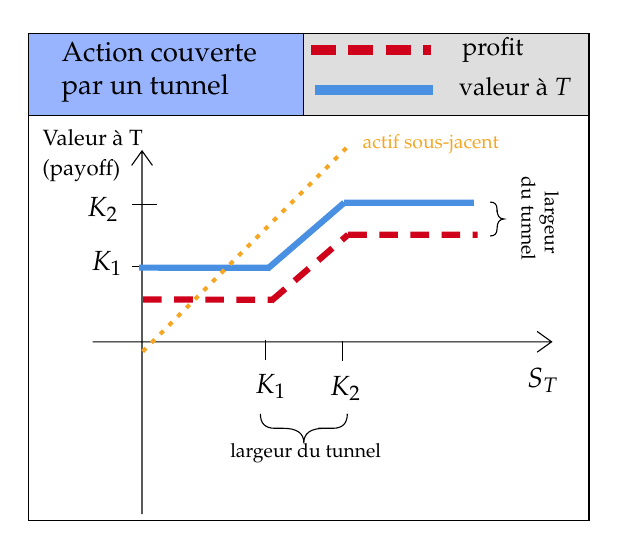
\begin{tikzpicture}[x=0.75pt,y=0.75pt,yscale=-1,xscale=1]
%uncomment if require: \path (0,349); %set diagram left start at 0, and has height of 349

%Shape: Rectangle [id:dp02624018355068425] 
\draw   (336,39.33) -- (606.17,39.33) -- (606.17,273.67) -- (336,273.67) -- cycle ;
%Shape: Rectangle [id:dp42550263898781093] 
\draw  [fill={rgb, 255:red, 152; green, 180; blue, 255 }  ,fill opacity=1 ] (336,39.33) -- (598.17,39.33) -- (598.17,78.67) -- (336,78.67) -- cycle ;
%Shape: Rectangle [id:dp019016078913590695] 
\draw  [fill={rgb, 255:red, 222; green, 222; blue, 222 }  ,fill opacity=1 ] (468.5,39.24) -- (606.17,39.24) -- (606.17,78.67) -- (468.5,78.67) -- cycle ;
%Straight Lines [id:da9746521197693616] 
\draw [color={rgb, 255:red, 208; green, 2; blue, 27 }  ,draw opacity=1 ][line width=3.75]  [dash pattern={on 9pt off 4.5pt}]  (472.2,47.11) -- (529.87,47.11) ;
%Straight Lines [id:da21520173766895323] 
\draw [color={rgb, 255:red, 74; green, 144; blue, 226 }  ,draw opacity=1 ][line width=3.75]    (474.17,66.33) -- (531.17,66.33) ;
%Shape: Axis 2D [id:dp9458670686230795] 
\draw  (367,187.67) -- (588.17,187.67)(390.83,95.67) -- (390.83,270.67) (581.17,182.67) -- (588.17,187.67) -- (581.17,192.67) (385.83,102.67) -- (390.83,95.67) -- (395.83,102.67)  ;
%Straight Lines [id:da46034392012067693] 
\draw    (385.83,151.33) -- (397.83,151.33) ;
%Straight Lines [id:da25541970441950257] 
\draw    (487.25,196.7) -- (487.25,187.05) ;
%Straight Lines [id:da5840111395603904] 
\draw    (450.5,196.65) -- (450.5,187) ;
%Straight Lines [id:da3398468398362082] 
\draw [color={rgb, 255:red, 74; green, 144; blue, 226 }  ,draw opacity=1 ][line width=2.25]    (488.25,120.64) -- (550.69,120.69) ;
%Straight Lines [id:da766471031454568] 
\draw [color={rgb, 255:red, 74; green, 144; blue, 226 }  ,draw opacity=1 ][line width=2.25]    (451.12,152.62) -- (488.25,120.64) ;
%Straight Lines [id:da8179350208142249] 
\draw [color={rgb, 255:red, 74; green, 144; blue, 226 }  ,draw opacity=1 ][line width=2.25]    (389.45,151.92) -- (451.88,151.96) ;
%Straight Lines [id:da15703311440320822] 
\draw [color={rgb, 255:red, 208; green, 2; blue, 27 }  ,draw opacity=1 ][line width=2.25]  [dash pattern={on 6.75pt off 4.5pt}]  (490.12,136.04) -- (552.55,136.08) ;
%Straight Lines [id:da2509003548986979] 
\draw [color={rgb, 255:red, 208; green, 2; blue, 27 }  ,draw opacity=1 ][line width=2.25]  [dash pattern={on 6.75pt off 4.5pt}]  (452.99,168.01) -- (490.12,136.04) ;
%Straight Lines [id:da8299907131334008] 
\draw [color={rgb, 255:red, 208; green, 2; blue, 27 }  ,draw opacity=1 ][line width=2.25]  [dash pattern={on 6.75pt off 4.5pt}]  (391.31,167.31) -- (453.75,167.36) ;
%Straight Lines [id:da6108319797175599] 
\draw [color={rgb, 255:red, 245; green, 166; blue, 35 }  ,draw opacity=1 ][line width=1.5]  [dash pattern={on 1.69pt off 2.76pt}]  (391.17,192.33) -- (491.17,92.33) ;
%Shape: Brace [id:dp1095359743364297] 
\draw   (447.83,222.33) .. controls (447.83,227) and (450.16,229.33) .. (454.83,229.33) -- (458.78,229.33) .. controls (465.45,229.33) and (468.78,231.66) .. (468.78,236.33) .. controls (468.78,231.66) and (472.11,229.33) .. (478.78,229.33)(475.78,229.33) -- (482.73,229.33) .. controls (487.4,229.33) and (489.73,227) .. (489.73,222.33) ;
%Straight Lines [id:da5856705496016874] 
\draw    (385.83,121.33) -- (397.83,121.33) ;
%Shape: Brace [id:dp8659015694536814] 
\draw   (558.5,136.67) .. controls (560.74,136.67) and (561.86,135.55) .. (561.86,133.3) -- (561.86,133.3) .. controls (561.86,130.1) and (562.98,128.5) .. (565.23,128.5) .. controls (562.98,128.5) and (561.86,126.9) .. (561.86,123.7)(561.86,125.14) -- (561.86,123.7) .. controls (561.86,121.45) and (560.74,120.33) .. (558.5,120.33) ;

% Text Node
\draw (399.08,57.73) node   [align=left] {Action couverte \\par un tunnel};
% Text Node
\draw (559.88,46.82) node  [font=\small] [align=left] {profit};
% Text Node
\draw (570.64,64.93) node  [font=\small] [align=left] {valeur à $\displaystyle T$};
% Text Node
\draw (584,206) node   [align=left] {$\displaystyle S_{T}$};
% Text Node
\draw (374,150) node   [align=left] {$\displaystyle K_{1}$};
% Text Node
\draw (367,98) node  [font=\small,rotate=-0.4] [align=left] {{\footnotesize Valeur à T }\\{\footnotesize (payoff)}};
% Text Node
\draw (453,209) node   [align=left] {$\displaystyle K_{1}$};
% Text Node
\draw (489,210) node   [align=left] {$\displaystyle K_{2}$};
% Text Node
\draw (530,92.33) node   [align=left] {\textcolor[rgb]{0.96,0.65,0.14}{{\scriptsize actif sous-jacent}}};
% Text Node
\draw (469.67,241.33) node   [align=left] {{\scriptsize largeur du tunnel}};
% Text Node
\draw (372,124) node   [align=left] {$\displaystyle K_{2}$};
% Text Node
\draw (587,130.33) node  [rotate=-90] [align=left] {{\scriptsize largeur}};
% Text Node
\draw (577,128.33) node  [rotate=-90] [align=left] {{\scriptsize du tunnel}};


\end{tikzpicture}
\end{center}

\begin{align*}
	\text{tunnel}
	&= 	P(K_1) - C(K_2)	\\
	\text{\textcolor{burntorange}{action couverte} par un tunnel}
	&= 	P(K_1) - C(K_2)	+ \textcolor{burntorange}{S_{T}} \\
\end{align*}

Si l'on achète deux options ayant la même prime, on obtient un tunnel à prime zéro. Par exemple, on vend une option d'achat $C(120) = 5$ et achète une option de vente $-P(120) = -5$ ayant donc un coût initial nul.
\end{definitionNOHFILL}

\columnbreak
\subsection{Spéculation sur la volatilité}
\begin{definitionNOHFILL}[\textbf{Stellage} \og \textit{straddle} \fg{}]
Créé en achetant une option de vente et une option d'achat avec un prix d'exercice $K$.

\begin{distributions}[Contexte]
\begin{itemize}[leftmargin = *]
	\item	Souvent bâti avec un prix d'exercice au cours du marché (in-the-money);
	\item	L'idée est de faire un profit si le prix de l'actif sous-jacent \textbf{baisse ou descend};
	\item	Son avantage est donc qu'il peut être profitable avec une baisse ou hausse du prix de l'actif sous-jacent;
	\item	Cependant, puisqu'il faut acheter deux options au cours du marché, le coût est plutôt élevé.
\end{itemize}
\end{distributions}

$\text{Straddle} = Put(K, T) + Call(K, T)$.\\

Il s'ensuit que la valeur à l'échéance est:
\begin{align*}
	|S_{T} - K|	
	&=	
		\begin{cases}
		(K - S_{T})	+	0	=	K - S_{T},	&	S_{T} \le K	\\
		0	+	(S_{T} - K)	=	S_{T} - K,	&	S_{T} >	K	\\
		\end{cases}
\end{align*}

\begin{center}
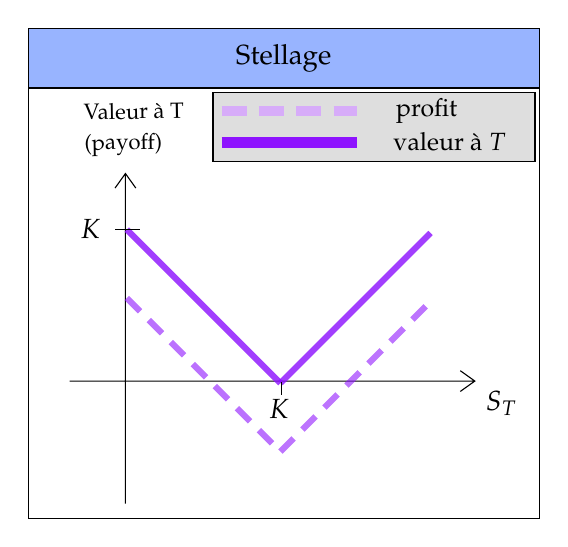
\begin{tikzpicture}[x=0.75pt,y=0.75pt,yscale=-1,xscale=1]
%uncomment if require: \path (0,281); %set diagram left start at 0, and has height of 281

%Shape: Axis 2D [id:dp8150307323595705] 
\draw  (49,192.33) -- (244.17,192.33)(75.83,92.33) -- (75.83,251.33) (237.17,187.33) -- (244.17,192.33) -- (237.17,197.33) (70.83,99.33) -- (75.83,92.33) -- (80.83,99.33)  ;
%Straight Lines [id:da9384465113929932] 
\draw [color={rgb, 255:red, 142; green, 19; blue, 254 }  ,draw opacity=0.82 ][line width=2.25]    (76.5,119.33) -- (150.5,193.33) ;
%Shape: Rectangle [id:dp9521369685676353] 
\draw   (29,22.33) -- (275.17,22.33) -- (275.17,258.33) -- (29,258.33) -- cycle ;
%Shape: Rectangle [id:dp8359683554212727] 
\draw  [fill={rgb, 255:red, 152; green, 180; blue, 255 }  ,fill opacity=1 ] (29,22.33) -- (275.17,22.33) -- (275.17,51.13) -- (29,51.13) -- cycle ;
%Shape: Rectangle [id:dp6862105279378832] 
\draw  [fill={rgb, 255:red, 222; green, 222; blue, 222 }  ,fill opacity=1 ] (118,53.33) -- (273.17,53.33) -- (273.17,86.33) -- (118,86.33) -- cycle ;
%Straight Lines [id:da14433777002766845] 
\draw [color={rgb, 255:red, 215; green, 172; blue, 249 }  ,draw opacity=1 ][line width=3.75]  [dash pattern={on 9pt off 4.5pt}]  (122.17,62.33) -- (187.17,62.33) ;
%Straight Lines [id:da897309116521503] 
\draw [color={rgb, 255:red, 142; green, 19; blue, 254 }  ,draw opacity=1 ][line width=3.75]    (122.17,77.33) -- (187.17,77.33) ;

%Straight Lines [id:da6723643933487031] 
\draw [color={rgb, 255:red, 142; green, 19; blue, 254 }  ,draw opacity=0.82 ][line width=2.25]    (150.5,193.33) -- (222.83,121) ;
%Straight Lines [id:da9747958724573911] 
\draw [color={rgb, 255:red, 142; green, 19; blue, 254 }  ,draw opacity=0.6 ][line width=2.25]  [dash pattern={on 6.75pt off 4.5pt}]  (76.5,152.33) -- (150.5,226.33) ;
%Straight Lines [id:da3459436058254277] 
\draw [color={rgb, 255:red, 142; green, 19; blue, 254 }  ,draw opacity=0.59 ][line width=2.25]  [dash pattern={on 6.75pt off 4.5pt}]  (150.5,226.33) -- (222.83,154) ;
%Straight Lines [id:da42512294493800273] 
\draw    (70.83,119.33) -- (82.83,119.33) ;
%Straight Lines [id:da2255022277875438] 
\draw    (150.83,199) -- (150.83,193) ;

% Text Node
\draw (257,203) node   [align=left] {$\displaystyle S_{T}$};
% Text Node
\draw (59,119) node   [align=left] {$\displaystyle K$};
% Text Node
\draw (80,71) node  [font=\small,rotate=-358.99] [align=left] {{\footnotesize Valeur à T }\\{\footnotesize (payoff)}};
% Text Node
\draw (152.08,36.73) node   [align=left] {Stellage};
% Text Node
\draw (232,77) node  [font=\small] [align=left] {valeur à $\displaystyle T$};
% Text Node
\draw (221,62) node  [font=\small] [align=left] {profit};
% Text Node
\draw (149.83,206) node   [align=left] {$\displaystyle K$};


\end{tikzpicture}
\end{center}
\end{definitionNOHFILL}


\begin{definitionNOHFILL}[\textbf{Stellage élargi} \og \textit{strangle} \fg{}]
Créé en 
\begin{itemize}[leftmargin = *]
	\item	achetant une option de vente avec un prix d'exercice $K_{1}$ et 
	\item	achetant une option d'achat avec un prix d'exercice $K_{2}$ où 
	\item	$K_{1} < K_{2}$.
\end{itemize}

\begin{distributions}[Contexte]
\begin{itemize}[leftmargin = *]
	\item	Pour réduire le coût des primes, les options sont à des prix d'exercice hors du cours du marché (out-of-the-money);
	\item	Cela réduit la perte maximale, mais augmente la variation nécessaire pour faire un profit.
\end{itemize}
\end{distributions}

$\text{Strangle} = Put(K_1, T) + Call(K_2, T)$.\\

Il s'ensuit que la valeur à l'échéance est:
\begin{align*}
		\begin{cases}
		(K_{1} - S_{T})	+	0	=	K_{1} - S_{T},	&	S_{T} \le K_{1}	\\
		0	+	0	=	0,	&	K_{1} < S_{T} \le K_{2} 	\\
		0	+	(S_{T} - K_{2})	=	S_{T} - K_{2},	&	S_{T} >	K_{2}	\\
		\end{cases}
\end{align*}

\begin{center}
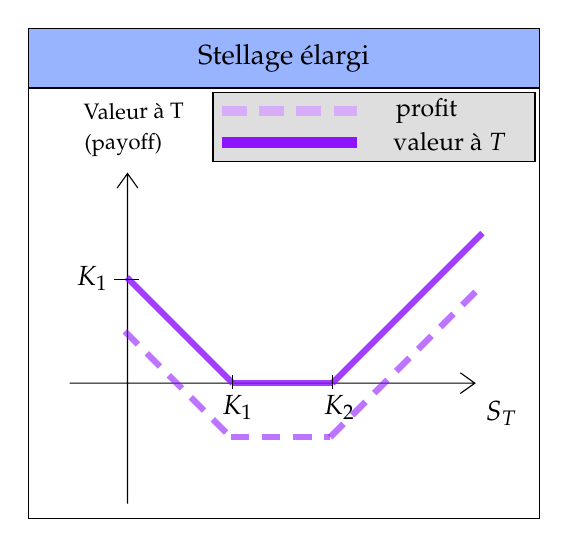
\begin{tikzpicture}[x=0.75pt,y=0.75pt,yscale=-1,xscale=1]
%uncomment if require: \path (0,281.3333320617676); %set diagram left start at 0, and has height of 281.3333320617676

%Shape: Axis 2D [id:dp09154892396952885] 
\draw  (317,193.33) -- (512.17,193.33)(344.83,92.33) -- (344.83,251.33) (505.17,188.33) -- (512.17,193.33) -- (505.17,198.33) (339.83,99.33) -- (344.83,92.33) -- (349.83,99.33)  ;
%Straight Lines [id:da6000960978699228] 
\draw [color={rgb, 255:red, 142; green, 19; blue, 254 }  ,draw opacity=0.82 ][line width=2.25]    (344.5,142.33) -- (395.5,193.33) ;


%Shape: Rectangle [id:dp44437730275029286] 
\draw   (297,22.33) -- (543.17,22.33) -- (543.17,258.33) -- (297,258.33) -- cycle ;
%Shape: Rectangle [id:dp7743472076958418] 
\draw  [fill={rgb, 255:red, 152; green, 180; blue, 255 }  ,fill opacity=1 ] (297,22.33) -- (543.17,22.33) -- (543.17,51.13) -- (297,51.13) -- cycle ;
%Shape: Rectangle [id:dp7779557733517186] 
\draw  [fill={rgb, 255:red, 222; green, 222; blue, 222 }  ,fill opacity=1 ] (386,53.33) -- (541.17,53.33) -- (541.17,86.33) -- (386,86.33) -- cycle ;
%Straight Lines [id:da9460151429343937] 
\draw [color={rgb, 255:red, 215; green, 172; blue, 249 }  ,draw opacity=1 ][line width=3.75]  [dash pattern={on 9pt off 4.5pt}]  (390.17,62.33) -- (455.17,62.33) ;


%Straight Lines [id:da07066423334519834] 
\draw [color={rgb, 255:red, 142; green, 19; blue, 254 }  ,draw opacity=1 ][line width=3.75]    (390.17,77.33) -- (455.17,77.33) ;



%Straight Lines [id:da6891207896917613] 
\draw [color={rgb, 255:red, 142; green, 19; blue, 254 }  ,draw opacity=0.82 ][line width=2.25]    (443.5,193.33) -- (515.83,121) ;


%Straight Lines [id:da9025524478967739] 
\draw    (338.5,143.33) -- (350.5,143.33) ;


%Straight Lines [id:da8837361321867341] 
\draw [color={rgb, 255:red, 142; green, 19; blue, 254 }  ,draw opacity=0.82 ][line width=2.25]    (395.5,193.33) -- (443.5,193.33) ;


%Straight Lines [id:da8842152242628301] 
\draw    (395.5,196.33) -- (395.5,189.33) ;


%Straight Lines [id:da3358507555044139] 
\draw    (443.5,196.33) -- (443.5,189.33) ;


%Straight Lines [id:da3055341213887268] 
\draw [color={rgb, 255:red, 142; green, 19; blue, 254 }  ,draw opacity=0.59 ][line width=2.25]  [dash pattern={on 6.75pt off 4.5pt}]  (343.5,168.33) -- (394.5,219.33) ;


%Straight Lines [id:da6895564400108751] 
\draw [color={rgb, 255:red, 142; green, 19; blue, 254 }  ,draw opacity=0.59 ][line width=2.25]  [dash pattern={on 6.75pt off 4.5pt}]  (442.5,219.33) -- (514.83,147) ;


%Straight Lines [id:da22060129362320668] 
\draw [color={rgb, 255:red, 142; green, 19; blue, 254 }  ,draw opacity=0.59 ][line width=2.25]  [dash pattern={on 6.75pt off 4.5pt}]  (394.5,219.33) -- (442.5,219.33) ;



% Text Node
\draw (525,208) node   [align=left] {$\displaystyle S_{T}$};
% Text Node
\draw (348,71) node  [font=\small,rotate=-358.99] [align=left] {{\footnotesize Valeur à T }\\{\footnotesize (payoff)}};
% Text Node
\draw (420.08,36.73) node   [align=left] {Stellage élargi};
% Text Node
\draw (500,77) node  [font=\small] [align=left] {valeur à $\displaystyle T$};
% Text Node
\draw (489,62) node  [font=\small] [align=left] {profit};
% Text Node
\draw (328,143) node   [align=left] {$\displaystyle K_{1}$};
% Text Node
\draw (447,205) node   [align=left] {$\displaystyle K_{2}$};
% Text Node
\draw (398,205) node   [align=left] {$\displaystyle K_{1}$};


\end{tikzpicture}
\end{center}
\end{definitionNOHFILL}

\begin{definitionNOHFILL}[Écart papillon \og \textit{Butterfly Spread (BFS)} \fg{} ]
Créé en 
\begin{itemize}[leftmargin = *]
	\item	achetant stellage élargi avec prix d'exercices $K_{1}$ et $K_{3}$;
	\item	vendant un stellage avec un prix d'exercice $K_{2}$; 
	\item	où $K_{1} < K_{2} < K_{3}$;
	\item	L'écart papillon	 est symétrique avec $K_{2} - K_{1} = K_{3} - K_{2}$.
\end{itemize}

$\text{BFS} = Put(K_1, T) + Call(K_3, T) - Put(K_2, T) - Call(K_2, T)$.

\textbf{Notes}
\begin{itemize}[leftmargin = *]
	\item	Il existe plusieurs façons de recréer un écart papillon;
	\item	Par exemple, un écart haussier aux prix d'exercice $K_{1}$ et $K_{2}$ combiné avec un écart baissier aux prix d'exercice $K_{2}$ et $K_{3}$.
\end{itemize}
$\text{BFS} = Call(K_1, T) - 2 Call(K_2, T) + Call(K_3, T)$.

\begin{center}
	

\tikzset{every picture/.style={line width=0.75pt}} %set default line width to 0.75pt        

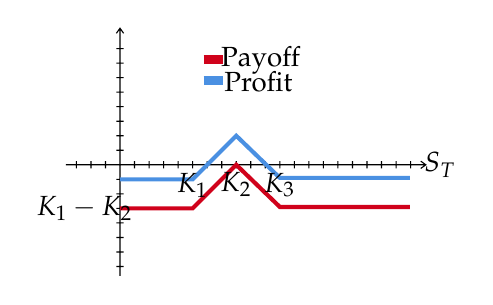
\begin{tikzpicture}[x=0.75pt,y=0.75pt,yscale=-0.35,xscale=0.35]
%uncomment if require: \path (0,363); %set diagram left start at 0, and has height of 363

%Shape: Axis 2D [id:dp516021239542077] 
\draw  (14,196) -- (509.5,196)(88.5,8) -- (88.5,349) (502.5,191) -- (509.5,196) -- (502.5,201) (83.5,15) -- (88.5,8) -- (93.5,15) (108.5,191) -- (108.5,201)(128.5,191) -- (128.5,201)(148.5,191) -- (148.5,201)(168.5,191) -- (168.5,201)(188.5,191) -- (188.5,201)(208.5,191) -- (208.5,201)(228.5,191) -- (228.5,201)(248.5,191) -- (248.5,201)(268.5,191) -- (268.5,201)(288.5,191) -- (288.5,201)(308.5,191) -- (308.5,201)(328.5,191) -- (328.5,201)(348.5,191) -- (348.5,201)(368.5,191) -- (368.5,201)(388.5,191) -- (388.5,201)(408.5,191) -- (408.5,201)(428.5,191) -- (428.5,201)(448.5,191) -- (448.5,201)(468.5,191) -- (468.5,201)(488.5,191) -- (488.5,201)(68.5,191) -- (68.5,201)(48.5,191) -- (48.5,201)(28.5,191) -- (28.5,201)(83.5,176) -- (93.5,176)(83.5,156) -- (93.5,156)(83.5,136) -- (93.5,136)(83.5,116) -- (93.5,116)(83.5,96) -- (93.5,96)(83.5,76) -- (93.5,76)(83.5,56) -- (93.5,56)(83.5,36) -- (93.5,36)(83.5,216) -- (93.5,216)(83.5,236) -- (93.5,236)(83.5,256) -- (93.5,256)(83.5,276) -- (93.5,276)(83.5,296) -- (93.5,296)(83.5,316) -- (93.5,316)(83.5,336) -- (93.5,336) ;
\draw   ;
%Straight Lines [id:da9881769874738698] 
\draw [color={rgb, 255:red, 208; green, 2; blue, 27 }  ,draw opacity=1 ][line width=3]    (203.5,51) -- (230.5,51) ;


%Straight Lines [id:da972554603165243] 
\draw [color={rgb, 255:red, 74; green, 144; blue, 226 }  ,draw opacity=1 ][line width=3]    (203.5,80) -- (230.5,80) ;



%Straight Lines [id:da5214606141485839] 
\draw [color={rgb, 255:red, 208; green, 2; blue, 27 }  ,draw opacity=1 ][line width=1.5]    (88.5,256) -- (188.5,256) -- (248.5,196) -- (308.5,254) -- (487.5,254) ;


%Straight Lines [id:da6207165128721853] 
\draw [color={rgb, 255:red, 74; green, 144; blue, 226 }  ,draw opacity=1 ][line width=1.5]    (88.5,216) -- (188.5,216) -- (248.5,156) -- (308.5,214) -- (487.5,214) ;



% Text Node
\draw (529,196) node  [align=left] {$\displaystyle S_{T}$};
% Text Node
\draw (282,52) node  [align=left] {Payoff};
% Text Node
\draw (279,81) node  [align=left] {Profit};
% Text Node
\draw (188.5,224) node   {$K_{1}$};
% Text Node
\draw (308.5,224) node   {$K_{3}$};
% Text Node
\draw (248.5,223) node   {$K_{2}$};
% Text Node
\draw (40,256) node   {$K_{1} -K_{2}$};


\end{tikzpicture}


\end{center}
\end{definitionNOHFILL}

\begin{definitionNOHFILL}[Écart papillon asymétrique]
\begin{itemize}[leftmargin = *]
	\item	La distinction avec un écart papillon symétrique est qu'on achète/vend en différentes proportions des options d'achat;
	\item	$\text{A-BFS} = mCall(K_1, T) - (m + n) Call(K_2, T) + n Call(K_3, T)$;
	\item	L'écart est asymétrique avec $m(K_{2} - K_{1}) = n(K_{3} - K_{2})$.
\end{itemize}

Puisque la différence en prix n'est pas symétrique, on fait une "interpolation" de sorte.\\

Pour calcule le nombre d'options à acheter/vendre aux différents prix:
\begin{enumerate}[leftmargin = *]
	\item	On calcule la différence en prix total $K_{3} - K_{1}$;
	\item	On calcule séparément les différences de prix:
		\begin{align*}
		K_{2} - K_{1}	\\
		K_{3} - K_{2}
		\end{align*}
	\item[]\textbf{Intuition}	La somme de ces deux différences résulte en l'écart total.
		\begin{align*}
		(K_{2} - K_{1}) +  (K_{3} - K_{2}) = (K_{3} - K_{1})
		\end{align*}
	\item	On :
		\begin{itemize}[leftmargin = *]
		\item	vends $K_{3} - K_{1}$ options au prix d'exercice $K_{2}$;
		\item	achète $K_{2} - K_{1}$ options au prix $K_{3}$;
		\item	achète $K_{3} - K_{2}$ options au prix $K_{1}$.
		\end{itemize}
	\item	Avec des options d'achat, on obtient:
		\begin{align*}
		 + (K_{3} - K_{2}) C(K_{1}) - (K_{3} - K_{1}) C(K_{2}) + (K_{2} - K_{1}) C(K_{3}) 
		\end{align*}
	\item[]\textbf{Intuition}	On peut donc pondérer par la différence totale et obtenir une "interpolation":
		\begin{align*}
		 + \frac{(K_{3} - K_{2})}{(K_{3} - K_{1})} C(K_{1}) - C(K_{2}) + \frac{(K_{2} - K_{1})}{(K_{3} - K_{1})} C(K_{3}) 
		\end{align*}
\end{enumerate}

C'est d'ici que provient la notation avec $\lambda$: 
\begin{align*}
	\lambda
	&=	\frac{K_{3} - K_{2}}{K_{3} - K_{1}}
\end{align*}
Pour chaque option avec un prix d'exercice de $K_{2}$ vendue, on achète $\lambda K_{1}$ et $(1 - \lambda) K_{3}$.
\end{definitionNOHFILL}

\newpage

\setcounter{section}{4}
\section{Contrats à terme}
\subsection{4 façons d'acheter une action}
Il y a plusieurs façons d'acheter une action et le prix va dépendre du \textbf{moment de paiement} et du \textbf{moment de la livraison}.
\begin{center}
\begin{tabular}{|>{\columncolor{airforceblue}}c	|	>{\columncolor{beaublue}}c	|	>{\columncolor{beaublue}}c	|	c	|}
\hline
\rowcolor{blue(matcha)}
	Contrat	&	\shortstack{Moment de\\ paiement}	&	\shortstack{Moment de\\ la livraison}	&	Paiement	\\\hline
	\textcolor{white}{\textbf{Outright purchase}}	&	0	&	0	&	$S_{0}$	\\\hline
	\textcolor{white}{\textbf{Forward contract}}		&	$T$	&	$T$	&	$F_{0, T}$	\\\hline
	\textcolor{white}{\textbf{Prepaid forward contract}}	&	0	&	$T$	&	$F_{0, T}^{P}$	\\\hline
	\textcolor{white}{\textbf{Fully leveraged purchase}}	&	$T$	&	0	&	$S_{0}\textrm{e}^{rT}$	\\\hline
\end{tabular}
\end{center}

\begin{description}
	\item[Achat pleinement par emprunt \og \textit{fully leveraged purchase} \fg{}]	On emprunte de l'argent pour obtenir l'actif immédiatement (à $t = 0$) en différant le paiement (remboursement) au temps $T$;
	\item[Contrat à terme de gré à gré prépayé \og \textit{prepaid forward contract} \fg{}]	On paye immédiatement (à $t = 0$) au prix $F_{0, T}^{P}$, mais on reçoit quand même l'actif plus tard.
\end{description}
Ce faisant, on s'attend à ce que $F_{0, T} = F_{0, T}^{P} \textrm{e}^{rT}$.

\begin{distributions}[Notation de prix]
\begin{description}
	\item[$F_{0, T}^{P}$:]	est le \textbf{prix à terme} d'un contrat à terme de gré à gré \textbf{prépayé};
	\item	$F_{0, T} = F_{0, T}^{P} \textrm{e}^{rT}$.
\end{description}
\end{distributions}

\begin{definitionNOHFILL}[La \textbf{loi du prix unique}]
Stipule que deux portefeuilles avec les mêmes profits doivent avoir le même prix.

Nous tarifions des contrats à terme de gré à gré \textit{prépayé}s et utilisons ces prix pour dériver les prix des contrats à terme de gré à gré. 
\end{definitionNOHFILL}

\columnbreak

\subsection{Tarification d'un \textbf{contrat à terme de gré à gré prépayé}}

Sans dividendes, le prix du contrat à terme de gré à gré prépayé est le prix de l'actif sous-jacent aujourd'hui---$S_{0}$. 

Si une action a des dividendes, elles seront payables au propriétaire de l'action. Puisque l'acheteur du contrat (position longue) va seulement posséder le contrat au temps $T$, il ne recevra pas de \textbf{dividendes}. Cela va donc faire \textbf{baisser la valeur de l'action} et le prix à terme du contrat devra le tenir en compte. Également, on présume que le \textbf{droit de vote n'a aucune valeur} pour calculer le prix à terme.\\

Dans le cas de \textbf{dividendes discrets}, il suffit de soustraire la valeur actualisée des dividendes: $F_{0, T}^{P} = S_{0} - PV(div)$. Ces dividendes sont supposés d'être réinvestis dans des obligations zéro coupon.

Un modèle de \textbf{dividendes payés continûment} suppose un taux de dividendes continûment composé $\delta$. Une part de l'action au temps initial devient $\textrm{e}^{\delta T}$ parts au temps $T$. Cependant, nous souhaitons avoir seulement une part au temps $T$ et donc achetons $\textrm{e}^{-\delta T}$ parts au début. Le prix du contrat est donc $F_{0, T}^{P} = S_{0} e^{-\delta T}$.

Dans le cas de dividendes \textbf{proportionnels}, on suppose qu'ils sont réinvestis dans le sous-jacent.
\begin{center}
	En bref:
\begin{tabular}{| >{\columncolor{beaublue}}c |	 >{\columncolor{beaublue}}c |	 >{\columncolor{beaublue}}c |}
\hline\rowcolor{airforceblue} 
	\textcolor{white}{\textbf{Dividendes}}	&	\textcolor{white}{\textbf{Prix à terme prépayé}}	&	\textcolor{white}{\textbf{Prix à terme}}	\\\specialrule{0.1em}{0em}{0.0em} 
Sans dividendes				&	$S_{0}$					&	$S_{0} e^{r T}$	\\\hline
Dividendes payés continument	&	$S_{0}e^{-\delta T}$		&	$S_{0} e^{(r - \delta) T}$	\\\hline
Dividendes discrets			&	$S_{0} - PV(div.)$	&	$S_{0} e^{r T} - FV(div.)$	\\\hline
\end{tabular}
\end{center}

\begin{definitionNOHFILL}[\textbf{Prime à terme} \og \textit{forward premium} \fg{} ]
Défini comme le ratio du prix à terme au prix courant de l'actif sous-jacent:
\begin{align*}
	\text{Prime à terme} = \frac{F_{0, T}}{S_{0}}
\end{align*}

La prime à terme annualisée (\og \textit{annualized forward premium} \fg{}) est $\frac{1}{T} \ln \left( \frac{F_{0, T}}{S_{0}}\right)$.

\end{definitionNOHFILL}

\begin{center}
	Est-ce de l'arbitrage?
	\begin{tabular}{| >{\columncolor{beaublue}}c | >{\columncolor{beaublue}}c | >{\columncolor{beaublue}}c |}
	\hline\rowcolor{airforceblue} 
		\textcolor{white}{\textbf{Flux monétaires}}	&	\textcolor{white}{\textbf{Oui}}	&	\textcolor{white}{\textbf{Non}}	\\
		Au temps $0$, est-ce que le flux monétaire net est $\ge 0$?	&	X	&		\\\hline
		Est-ce que tous les flux monétaires nets futurs sont $\ge 0$?	&	X	&		\\\hline
		Est-ce qu'au moins un des flux monétaires nets futurs est $> 0$?	&	X	&		\\\hline
	\end{tabular}
\end{center}
Si la réponse à toutes les questions est oui, alors il y a une opportunité d'arbitrage. Pour identifier les flux monétaires, on utilise l'approche à deux étapes:
\begin{enumerate}
	\item	Écrire, sous forme d'inégalité, ce qui est observé;
	\item	Déplacer tout ce qui est sur le côté inférieur ($<$) au côté supérieur ou égal ($\ge$);
	\item[]	Nous avons les signes appropriés pour les transactions.
\end{enumerate}

\begin{definitionNOHFILL}[\textbf{Position synthétique}]
Une position synthétique réplique la valeur à l'échéance d'une autre position.

\tcbline

\begin{center}
	\textbf{Achat d'action synthétique}
\end{center}

On peut synthétiquement répliquer l'achat d'une action en prêtant de l'argent et achetant un contrat à terme de gré à gré.
\begin{center}
\begin{tabular}{| >{\columncolor{beaublue}}c |	c	|	c	|}
\hline\rowcolor{airforceblue} 
	\textcolor{white}{\textbf{Transaction}}	&	\textcolor{white}{\textbf{$t = 0$}}	&	\textcolor{white}{\textbf{$t = T$}}	\\\specialrule{0.1em}{0em}{0.0em} 
Prêt de $S_{0}\textrm{e}^{-\delta T}$	&	$-S_{0}\textrm{e}^{-\delta T}$	&	$+S_{0}\textrm{e}^{(r - \delta) T} = F_{0, T}$	\\\hline
\shortstack{Achat d'un contrat à\\ terme de gré à gré}	&	$0$	&	$S_{T} - F_{0, T}$	\\\specialrule{0.1em}{0em}{0.0em} 
Net	&	$-S_{0}\textrm{e}^{-\delta T}$	&	$S_{T}$	\\\specialrule{0.1em}{0em}{0.0em} 
\end{tabular}
\end{center}

\tcbline

\begin{center}
	\textbf{Obligation zéro-coupon synthétique}
\end{center}

On peut créer une obligation zéro-coupon synthétique en achetant une action et vendant un contrat à terme de gré à gré.
\begin{center}
\begin{tabular}{| >{\columncolor{beaublue}}c |	c	|	c	|}
\hline\rowcolor{airforceblue} 
	\textcolor{white}{\textbf{Transaction}}	&	\textcolor{white}{\textbf{$t = 0$}}	&	\textcolor{white}{\textbf{$t = T$}}	\\\specialrule{0.1em}{0em}{0.0em} 
Achat de $\textrm{e}^{-\delta T}$ actions	&		$-S_{0}\textrm{e}^{-\delta T}$	&	$+S_{T}$	\\\hline
\shortstack{Vente d'un contrat à\\ terme de gré à gré}	&	$0$	&	$F_{0, T} - S_{T}$	\\\specialrule{0.1em}{0em}{0.0em} 
Net	&	$0$	&	$F_{0, T} = S_{0}\textrm{e}^{(r - \delta)T}$	\\\specialrule{0.1em}{0em}{0.0em} 
\end{tabular}
\end{center}

Le rendement de cette stratégie s'appelle le \textbf{taux de mise en pension implicite} (\og \textit{implied repo rate} \fg{}). Cela signifie le taux implicite dans cette stratégie pour répliquer un rendement équivalent à une obligation zéro-coupon.
\end{definitionNOHFILL}

\begin{definitionNOHFILL}[\textbf{Contrat à terme synthétique} \og \textit{synthetic forward} \fg{}]
Un contrat à terme synthétique réplique la valeur à l'échéance d'un contrat à terme sans réellement en signer un.

Avec un \textbf{vrai} contrat à terme:
\begin{itemize}[leftmargin = *]
	\item	le coût initial est nul et
	\item	la valeur à l'échéance est l'écart entre le prix à terme et la valeur du sous-jacent ($S_{T} - F_{0, T}$).
\end{itemize}

Avec un contrat à terme \textbf{synthétique}:
\begin{itemize}[leftmargin = *]
	\item	on prévoit l'échange du bien contre un prix quelconque $K$ et 
	\item	la valeur à l'échéance est leur écart ($S_{T} - K$).
	\item	Il s'ensuit que le coût initial ne peut être nul et 
	\item	c'est pourquoi on \textbf{emprunte de l'argent}, ou de façon équivalente, \textbf{vend une obligation zéro-coupons}.
\end{itemize}

En bref, on \textbf{achète l'actif} et \textbf{emprunte de l'argent}:
\begin{center}
	\begin{tabular}{| >{\columncolor{beaublue}}c | >{\columncolor{beaublue}}c | >{\columncolor{beaublue}}c |}
	\hline\rowcolor{airforceblue} 
		\textcolor{white}{\textbf{Transaction}}	&	\textcolor{white}{\textbf{Flux au temps $0$}}	&	\textcolor{white}{\textbf{Flux au temps $T$}}	\\
		Acheter un actif			&	$-S_{0}$	&	$+S_{t}$	\\
		Emprunter de l'argent	&	$+S_{0}$	&	$-S_{0}\textrm{e}^{rT} = -F_{0, T}$	\\\hline
		Net des flux monétaires	&	$0$	&	$S_{t} - F_{0, T}$	\\\hline
	\end{tabular}
\end{center}

Le montant du prêt n'a pas besoin d'être $S_{0}$ puisque le contrat est synthétique. Ce faisant, si le montant emprunté d'un contrat est de $S_{0}$ on qu'il est au cours du marché.
\end{definitionNOHFILL}

\begin{definitionNOHFILL}[Comptant terme \og \textit{\textbf{Cash-and-carry}} \fg{}]
Dans un comptant terme, alias l'achat au comptant - vente à terme, achète une action avec un emprunt et vend un contrat à terme de gré à gré.\\

La stratégie s'apparente à une obligation zéro coupon financé par une obligation zéro coupon. Il s'ensuit que, sans arbitrage, le profit sera nul.
\begin{center}
\begin{tabular}{| >{\columncolor{beaublue}}c |	c	|	c	|}
\hline\rowcolor{airforceblue} 
	\textcolor{white}{\textbf{Transaction}}	&	\textcolor{white}{\textbf{$t = 0$}}	&	\textcolor{white}{\textbf{$t = T$}}	\\\specialrule{0.1em}{0em}{0.0em} 
Achat de $\textrm{e}^{-\delta T}$ actions	&		$-S_{0}\textrm{e}^{-\delta T}$	&	$+S_{T}$	\\\hline
\shortstack{Vente d'un contrat à\\ terme de gré à gré}	&	$0$	&	$F_{0, T} - S_{T}$	\\\hline
Emprunt de $S_{0}\textrm{e}^{-\delta T}$	&	$+S_{0}\textrm{e}^{-\delta T}$	&	$-S_{0}\textrm{e}^{(r - \delta) T}$	\\\specialrule{0.1em}{0em}{0.0em} 
Net	&	$0$	&	$F_{0, T} - S_{0}\textrm{e}^{(r - \delta) T}$	\\\specialrule{0.1em}{0em}{0.0em} 
\end{tabular}
\end{center}

Sans arbitrage, la dernière ligne s'annule.

\tcbline
L'inverse arrive lorsque le marché offre un contrat à terme de gré à gré sous-évalué.
\end{definitionNOHFILL}

\columnbreak

\subsection{Contrats de change}
\begin{distributions}[Notation de devises]
\begin{description}
	\item[DD] \textbf{Devise domestique} (ou de départ);
	\item[DÉ] \textbf{Devise étrangère};
	\item[$i_{D}$]	taux d'intérêt dans la DD;
	\item[$i_{\text{É}}$]	taux d'intérêt dans la DÉ;
	\item[$F_{0, T}^{P}$:]	est le prix d'un contrat de change à terme prépayé en DD;
	\begin{align*}
	F_{0, T}^{P} &= x_{0}(1 + i_{\text{É}})^{-T}\text{DD}
	\end{align*}		
	\item[$F_{0, T}$:]	est le prix d'un contrat de change à terme en DD;
	\begin{align*}
	F_{0, T} &= x_{0}(1 + i_{\text{É}})^{-T}(1 + i_{\text{D}})^{T}\text{DD}	
	\end{align*}		
	\item[$x_{t}$]	taux de change au temps $t$ en DD/DÉ
		\begin{itemize}[leftmargin = *]
		\item	Par exemple, $x_{0} = \frac{2\$}{\text{1\euro}} = \left(2 \frac{\$}{\text{\euro}}\right) \equiv \frac{2\text{DD}}{1\text{DÉ}}$
		\end{itemize}
\end{description}

La logique des formules des contrats à terme de gré à gré est:
\begin{align*}
	F_{0, T}^{P}(1 \text{DÉ})
	&=	\left(1\text{DÉ} \cdot \textrm{e}^{-i_{\text{DÉ}}T}\right) \cdot \left( x_{0}\frac{\text{DD}}{\text{DÉ}} \right)	
	=	x_{0} \cdot \textrm{e}^{-i_{\text{DÉ}}T}\text{DD}
\end{align*}
\end{distributions}

Un actif peut avoir un prix défini dans n'importe quelle devise; on dit qu'il est \og \textit{denominated} \fg{} dans cette devise.

\begin{definitionNOHFILL}[Contrat de change synthétique]
\begin{enumerate}
	\item	Emprunt de $x_0(1 + i_{\text{É}})^{-T}\text{DD}$ au taux $i_D$;
	\item 	Convertir les DD en DÉ;
	\item	Dépôt de $(1 + i_{É})^{-T}\text{DÉ}$ (au taux $i_{É}$) de 0 à $T$.
\end{enumerate}
La valeur à l'échéance sera $x_t - x_0 \left(\frac{1 + i_D}{1 + i_{\text{É}}}\right)^{T}$.
\end{definitionNOHFILL}

%%%	------------------------------------------------------------
%%%	NOTES:
%%%	+	Pas dans le cadre du cours d'hiver 2020 (AJVR).
%\subsection*{Calcul avec prime de risque et nuance}
%\begin{itemize}
%\item Certains sous-jacent ont une composante de risque non-négligeable. Or, on ne peut pas dire que $F_{0,T} = \esp{S_T}$. Toutefois,
%\[F_{0,T} = \esp{S_T} e^{-(\alpha - r) T}\]
%\end{itemize}
%où $\alpha$ est la prime de risque 	qu'on enlève pour obtenir le prix du Forward, tel que
%\[\alpha = \underbrace{r}_{\text{Taux sans risque}} + \underbrace{(\alpha - r)}_{\text{Prime de risque}}\]
%%%	------------------------------------------------------------
\columnbreak

\subsection{Contrat à terme standardisé}

Les contrats à terme standardisés sont transigés à la bourse. Ces transactions peuvent avoir lieu soit sur le plancher ou électroniquement.

\begin{definitionNOHFILL}[Contrat à terme standardisé \og \textit{future contract} \fg{}]
Différences des contrats à terme standardisés aux contrats à terme de gré à gré:
\begin{enumerate}[leftmargin = *]
	\item	\textbf{Personnalisable};
		\begin{itemize}[leftmargin = *]
		\item	Les contrats \og \textit{forwards} \fg{} peuvent être \textbf{faits de gré à gré} sur n'importe quel actif avec n'importe quelle clause et/ou condition;
		\item[]	L'acheteur et le vendeur peuvent choisir n'importe quel prix, montant, date d'échéance ou actif sous-jacent;	
		\item	Les contrats \og \textit{futures} \fg{} sont \textbf{surveillés et contrôlés} par des instances officielles au même titre que la bourse;
		\item[]	On dit donc qu'ils sont \textbf{standardisés}.
		\end{itemize}
	\item	\textbf{Valorisation au prix du marché} \og \textit{Marked-to-Market} \fg{};
		\begin{itemize}[leftmargin = *]
		\item	Pour un \og \textit{forward} \fg{}, toutes les échanges d'argent se produisent à l'échéance (le contrat est réglé à l'échéance);	
		\item	Pour un \og \textit{future} \fg{}, les pertes et profits sont réglés tous les jours (processus de valorisation au prix du marché) en espèces.
		\end{itemize}
	\item	\textbf{Risque de défaut};
		\begin{itemize}[leftmargin = *]
		\item	Pour un \og \textit{forward} \fg{}, le contrat est pleinement exposé au risque de défaut; 
		\item	Pour un \og \textit{future} \fg{}, avec le règlement quotidien des pertes et profits, le risque de défaut est minimisé.
		\end{itemize}
	\item	\textbf{Liquidité}: fait référence à l'aise d'acheter ou de vendre un actif ou, de façon équivalente, de sortir ou entrer de leur position;
		\begin{itemize}[leftmargin = *]
		\item	Pour un \og \textit{forward} \fg{}, il est impossible de sortir d'un contrat et donc ils ne sont pas liquides;
		\item	Pour un \og \textit{future} \fg{}, puisqu'ils sont transigés sur les marchés boursiers, ils sont liquides.
		\end{itemize}
	\item	\textbf{Limite de prix};
		\begin{itemize}[leftmargin = *]
		\item	Pour un \og \textit{forward} \fg{}, il n'y a aucune limite de prix sur l'actif sous-jacent et il peut varier sans limites;
		\item	Pour un \og \textit{future} \fg{}, il y a des limites incluses dans le contrat sur la variation du prix du sous-jacent;
		\item	Par exemple, s'il y a une baisse de 13\% au S \& P 500, il y a un \og \textit{circuit breaker} \fg{} qui arrête temporairement l'échange.
		\end{itemize}
\end{enumerate}

Puisque le règlement des contrats à terme standardisé est quotidien alors que le règlement des contrats à terme de gré à gré s'effectue à l'échéance, le prix à terme est différent.
\end{definitionNOHFILL}

\begin{definitionNOHFILL}[Marges initiales et de maintien \og \textit{initial and maintenance margins} \fg{}]
\begin{description}
	\item[Compte]	Afin de contrer le risque de défaut, l'acheteur et le vendeur doivent déposer de l'argent dans un compte (\og a \textit{margin account} \fg{}) accumulant de l'intérêt;
	\item[Marge initiale]	Le dépôt initial est nommé la marge initiale (\og \textit{inital margin} \fg{});
	\item[Marge de maintien]Les pertes et profits sont soustraits du compte et donc un niveau minimal est requis---la marge de maintien (\og \textit{maintenance margin} \fg{});
	\item[Appel de marge]	Si le montant dans le compte descend en dessous de la marge de maintien, nous recevons un appel de marge (\og \textit{margin call} \fg{}) qu'il faut y ajouter des fonds pour ramener la balance à la \textbf{marge initiale}.
\end{description}
\end{definitionNOHFILL}

\begin{formula}{Exemple de contrat à terme standardisé (\og \textit{futures contract} \fg{})}
On suppose l'achat d'une action se transigeant au prix de 950\$ aujourd'hui ($S_{0}$) ayant 250 parts sous-jacentes. La force d'intérêt ($\delta$) est de 6\%, la marge initiale égale à 80\% de la valeur notionnelle et la marge de maintien 10\% de la marge initiale.	\\

Au début, on doit établir la marge et sa balance initiale.
\begin{enumerate}
	\item	Premièrement, on trouve la valeur notionnelle : 
		\begin{align*}
		\underset{\text{\shortstack{nombre\\ sous-jacent}}}{\underbrace{250}} \times
			\underset{\text{nombre acheté}}{\underbrace{10}} \times 
			\underset{\text{prix inital}}{\underbrace{950\$}}
			&=	2\ 375\ 000\$
		\end{align*}
	\item	Puis, la marge initiale est 10\% de la valeur notionnelle : 
		\begin{align*}
		\underbrace{2\ 375\ 000\$}_{\text{valeur notionnelle}}\times 
		\underbrace{0.10}_{\text{\shortstack{taux de\\ marge initale}}}
		&=	237\ 500\$
		\end{align*}
	\item	Finalement, la marge de maintien est 80\% de la marge initiale :
		\begin{align*}
		\underbrace{237\ 500\$}_{\text{marge initiale}}	\times 
		0.80
		&=	190\ 000\$
		\end{align*}
\end{enumerate}


Si nous désirons rebalancer le portefeuille dans une semaine avec $F_{1/52, T}	=	930\$$ : 
\begin{enumerate}
	\item	On accumule la balance de la marge : 
		\begin{align*}
		\underbrace{237\ 500\$}_{\text{balance de la marge}} \times
		\underbrace{\textrm{e}^{0.06 (1/52)}}_{\shortstack{intérêt accumulé sur\\ une semaine}}
		&=	237\ 774.1966\$
		\end{align*}
	\item	Puis, on calcule le profit (ou la perte) :
		\begin{align*}
		\underbrace{250}_{\shortstack[c]{nombre\\ sous-jacent}} \times
		\underbrace{10}_{\text{nombre acheté}} \times 
		\underbrace{(930 -  950)}_{\shortstack[c]{profit par action\\ dans une semaine}}
		&=	-50\ 000\$
		\end{align*}
\end{enumerate}

En combinant la valeur accumulé de balance de la marge et le profit sur l'action, la \textbf{balance de la marge} dans une semaine est : $237\ 774.1966 + -50\ 000\$	=	187\ 774.1966\$$. Cependant, la balance est inférieure à la marge de maintien de $190\ 000\$$ ! Il y aura donc un \textbf{appel de marge} afin de remonter la balance de la marge à \textbf{la marge initiale} de $237\ 500\$$.	\\

Donc, l'investisseur débourse $237\ 500\$	-	187\ 774.1966\$	=	49\ 725.8034\$$ pour remonter la balance de la marge à $237\ 500\$$.
\end{formula}

\paragraph*{Note}	Le S \& P 500 a 250 parts sous-jacentes.

\newpage

% --- Chapitre 9 ---
\setcounter{section}{8}
\section{Parité et autres liens entre les options}
\begin{rappel}{Équation de parité des options vente-achat}
\begin{align*}
	C_{\text{Eur}}(K, T) - P_{\text{Eur}}(K, T)
	&=	F_{0, T}^{P}(S) - K\textrm{e}^{-rT}\\
\end{align*}

En anglais c'est le \og \textit{\textbf{Put-Call Parity Equation}} \fg{}. Cette équation vaut pour les options européennes seulement puisque les américaines peuvent être exercées à n'importe quel moment.
\end{rappel}

\subsection{Positions synthétiques}

Avec l'équation de parité, on peut créer des options, actions ou obligations zéro-coupon synthétiques.

\textbf{Option d'achat}
\begin{align*}
	-C(S, K)	
	&=	\underset{\text{\shortstack{achat d'une option\\ de vente équivalente}}}{\underbrace{-P(S, K)}} \;
		\underset{\text{\shortstack{achat d'une part\\ de l'action}}}{\underbrace{-F_{0, T}^{P}(S)}} \;
		\underset{\text{\shortstack{emprunt de $Ke^{-rT}$\\ au taux sans risque}}}{\underbrace{+K\textrm{e}^{-rT}}}
\end{align*}

\textbf{Option de vente}
\begin{align*}
	-P(S, K)	
	&=	\underset{\text{\shortstack{achat d'une option\\ d'achat équivalente}}}{\underbrace{-C(S, K)}} \;
		\underset{\text{\shortstack{vente d'une part\\ de l'action}}}{\underbrace{+F_{0, T}^{P}(S)}} \;
		\underset{\text{\shortstack{pret de $Ke^{-rT}$\\ au taux sans risque}}}{\underbrace{-K\textrm{e}^{-rT}}}
\end{align*}

\textbf{Action}
\begin{align*}
	-S_{0}
	&=	\underset{\text{\shortstack{vente de $e^{\delta T}$\\ options de vente}}}{\underbrace{+\textrm{e}^{\delta T} P(S. K)}} \;
		\underset{\text{\shortstack{achat de $e^{\delta T}$\\ options d'achat}}}{\underbrace{-\textrm{e}^{\delta T} C(S, K)}} \;
		\underset{\text{\shortstack{pret de $Ke^{-(r - \delta)T}$\\ au taux sans risque}}}{\underbrace{-K\textrm{e}^{-(r - \delta)T}}}
\end{align*}

\textbf{Bon du Trésor} (\og \textit{Treasury Bill (T-Bill)} \fg{})
\begin{align*}
	-K \textrm{e}^{-r T}
	&=	\underset{\text{\shortstack{vente d'une\\ option d'achat}}}{\underbrace{+C(S; K)}} \;
		\underset{\text{\shortstack{achat d'une\\ option de vente}}}{\underbrace{-P(S; K)}} \;
		\underset{\text{\shortstack{achat de $e^{-\delta T}$\\ parts de l'action}}}{\underbrace{-S_{0}\textrm{e}^{-\delta T}}}
\end{align*}

\columnbreak
\subsection{Parité des options}

\subsubsection*{Parité des options sur devises}
\begin{description}
	\item[$C(x_0, K, T)$]	Option d'achat qui permet d'acheter une unité de DÉ pour K unités de DD à l'échéance $T$;
	\item[$P(x_0, K, T)$] 	Option de vente qui permet d'acheter une unité de DÉ pour K unités de DD à l'échéance $T$.
\end{description}

Alors, on peut réécrire l'équation de parité : 
\begin{align*}
	C(x_0, K,T) - P(x_0, K, T) 
	&= 	x_0 (1 + i_{\text{É}})^{-T} - K(1 + i_D)^{-T}
\end{align*}

\subsubsection*{Parité des options sur obligation}
\begin{description}
	\item[$B_{0}$]	Prix aujourd'hui ($t = 0$) d'une obligation avec coupons;
	\item[$F_{0, T}^{P}(B)$]	Prix d'un contrat à terme standardisé prépayé sur une obligation avec coupons.
		\setlength{\mathindent}{-1cm}
		\begin{align*}
		F_{0, T}^{P}(B) 
		&=	B_{t} - PV(\text{coupons})
		\end{align*}
		\setlength{\mathindent}{1cm}
\end{description}

Alors, on peut réécrire l'équation de parité : 
\begin{align*}
	C(B_{0}, K, T) - P(B_{0}, K, T) 
	&= 	F_{0, T}^{P}(B) - F_{0, T}^{P}(K)
\end{align*}

\subsubsection*{Parité généralisée et option d'échange}
On peut généraliser toute option comme étant l'option d'échanger des actifs---l'\textit{actif sous-jacent} et l'\textit{actif d'exercice}---que l'on nomme des \textbf{options d'échange}.\\

Les options d'achat et de vente sont donc des options d'échange avec de l'argent comme actif d'exercice. On généralise d'abord la notation au-delà du concept d'achat et de vente pour un certain prix:
\begin{rappel_enhanced}[Notation]
\begin{description}
	\item[$C(S, K)$:] Permet au détenteur de l'option d'achat de recevoir $S$ en échange de $K$;
	\item[$P(S, K)$:] Permet au détenteur de l'option de vente de recevoir $K$ en échange de $S$.
\end{description}
\end{rappel_enhanced}

On peut penser à cette notation comme $C(\text{Receive}, \text{Give up})$ et $P(\text{Receive}, \text{Give up})$. Dans les deux cas, la valeur à l'échéance est $\max(0; \text{Receive} - \text{Give up})$.

\begin{rappel_enhanced}[Notation Claire]
\begin{description}
	\item[$S_{t}$:] Prix à $t$ de l'actif sous-jacent---le titre $A$;
	\item[$Q_{t}$:] Prix à $t$ du prix d'exercice---le titre $B$;
	\item[$C_{\text{euro}}(S_{t}, Q_{t}, T - t)$:] Permet, à $T$, d'achat le titre $A$ au prix du titre $B$;
	\item[$P_{\text{euro}}(S_{t}, Q_{t}, T - t)$:] Permet, à $T$, de vendre le titre $A$ au prix du titre $B$.
\end{description}
\end{rappel_enhanced}

\begin{rappel}{Équation de parité des options d'échange}
\begin{align*}
	C_{\text{euro}}(S_t, Q_t, T - t) - P_{\text{euro}}(S_t, Q_t, T-t) 
	&= 	F_{t,T}^{P}(S) - F_{t,T}^{P}(Q)
\end{align*}
\end{rappel}

%%%	------------
%%%	NOTE:
%%%	+	Sauté les notes de coaching pour les sous-sections sur:
%%%		Exchange Option Duality
%\begin{definitionNOHFILL}[Exchange option duality]
%By the law of one price, the two options $C(A, B)$ and $P(B, A)$ must have the same price : $C(A, B) = P(B, A)$.
%\end{definitionNOHFILL}
%%%		Put-Call Parity for Exchange Options
%%%		Scaling Exchange Options
%%%	------------

\subsubsection*{Options sur devise}
\begin{align*}
	C^{DD}(x_0, K, T) 
	&= 	K \cdot P^{DD}\left( \frac{1}{x_0}; \frac{1}{K}; T \right) 
	= 	x_0	K \cdot P^{\text{DÉ}} \left( \frac{1}{x_0}; \frac{1}{K}; T \right) \\
\end{align*}

\paragraph{Note}	Si le prix d'exercice est dans la même devise que le prix de l'option.

\columnbreak
\subsection{Comparaison de différentes options}

%%%	-----------------------------------
%%%	NOTE:
%%%	+	Ne fit pas ici, mais je pense qu'il faut le mettre quelque-part (AJVR).
%%%	
%\begin{rappel}{Intuition sur les options}
%Jusqu'ici les contrats étudiés ont été des engagements fermes---des contrats à termes de gré à gré (\og \textit{forward} \fg{}) ou standardisés (\og \textit{future} \fg{}). \\
%
%Ces contrats ne permettent pas aux deux parties de se retirer du contrat. L'aspect facultatif (\og \textit{optionability} \fg{}) est alors présent s'il est possible d'éviter des transactions non rentables.\\
%
%La question principale en tarification est donc:
%\begin{quotation}
%	Comment évaluer le droit de se retirer d'un engagement?
%\end{quotation}
%\end{rappel}
%%%	-----------------------------------

\subsubsection*{Considérations différents types d'options}

La première considération est que la valeur à l'échéance d'une option ne sera jamais négative puisqu'un investisseur \og rationnel \fg{} n'exercerait simplement pas l'option. L'émetteur de l'option va donc toujours demander une \textbf{prime positive} pour accepter ce risque de perte.\\

Donc les options américaines et européennes vont toujours avoir une \textbf{valeur d'au moins 0\$}:
\begin{align*}
	C(S, K, T) &\geq	0	&
	P(S, K, T) &\geq	0	
\end{align*}

Une option européenne peut uniquement être exercée à l'échéance alors qu'une option américaine peut être exercée à n'importe quel moment d'ici l'échéance. Il s'ensuit qu'une \textbf{option américaine vaut au moins autant qu'une option européenne}:
\begin{align*}
	C_{\text{amer}}(S, K, T)	&\geq	C_{\text{euro}}(S, K, T)	&
	P_{\text{amer}}(S, K, T)	&\geq	P_{\text{euro}}(S, K, T)	
\end{align*}

\subsubsection*{Bornes inférieures}
\paragraph{Option européenne}	Avec l'équation de parité des options vente-achat et que le coût ne peut pas être négatif, on obtient:

\begin{align*}
	C_{\text{euro}}(S, K, T)	
	&=	F_{0, T}^{P}(S) - K\textrm{e}^{-rT} \textcolor{teal}{+ P_{\text{euro}}(S, K, T)}	\\
	&\geq	\max\left(F_{0, T}^{P}(S) - K\textrm{e}^{-rT}; 0\right)	\\
	P_{\text{euro}}(S, K, T)	
	&=	F_{0, T}^{P}(S) - K\textrm{e}^{-rT} \textcolor{teal}{+ C_{\text{euro}}(S, K, T)}	\\
	&\geq	\max\left(K\textrm{e}^{-rT} - F_{0, T}^{P}(S); 0\right)
\end{align*}

\paragraph{Option américaine}	Une option américaine aura une valeur d'au moins l'option européenne. Également, puisqu'une option américaine peut être exercée à tout moment, sa valeur doit être au moins la valeur d'un exercice immédiat.

\paragraph{En bref}
\begin{rappel_enhanced}[Bornes inférieures options]
\begin{align*}
	C_{\text{amer}}(S, K, T)	\geq
	C_{\text{euro}}(S, K, T)	
	&\geq	\max\left(F_{0, T}^{P}(S) - K\textrm{e}^{-rT}; 0\right)	\\
	P_{\text{amer}}(S, K, T)	\geq
	P_{\text{euro}}(S, K, T)	
	&\geq	\max\left(K\textrm{e}^{-rT} - F_{0, T}^{P}(S); 0\right)
\end{align*}
et
\begin{align*}
	C_{\text{amer}}(S, K, T)	
	&\geq	S - K	&
	P_{\text{amer}}(S, K, T)
	&\geq	K - S
\end{align*}
\end{rappel_enhanced}

\subsubsection*{Bornes supérieures}
\begin{center}
	\textbf{Option américaine}
\end{center}

\paragraph{Option d'achat}
À son exercice, l'option permet d'obtenir l'actif sous-jacent. Si cette option coûtait plus que le prix du sous-jacent, on a simplement à l'acheter au lieu d'une option.\\

Ce faisant, \textcolor{cobalt}{la borne supérieure d'une option d'achat américaine est le prix au comptant (\og \textit{spot price} \fg{})}:
\begin{align*}
	S	
	\geq	C_{\text{amer}}(S, K, T)
	\geq	C_{\text{euro}}(S, K, T)
	\geq	\max\left(F_{0, T}^{P}(S) - K\textrm{e}^{-rT}; 0\right)
\end{align*}

\paragraph{Option de vente}
La valeur à l'échéance maximale d'une option de vente est le prix d'exercice $K$; lorsque la valeur de l'action est nulle on a $\max(K - 0; 0) = K$. Si le prix était supérieur à $K$, le vendeur n'aurait qu'à vendre son action directement sur le marché. \\

Ce faisant, \textcolor{cobalt}{la borne supérieure d'une option de vente américaine est le prix d'exercice}:
\begin{align*}
	K	
	\geq	P_{\text{amer}}(S, K, T)
	\geq	P_{\text{euro}}(S, K, T)
	\geq	\max\left(K\textrm{e}^{-rT} - F_{0, T}^{P}(S); 0\right)	
\end{align*}

\begin{center}
	\textbf{Option européenne}
\end{center}

\paragraph{Option d'achat}
La valeur à l'échéance sera au plus $\max(S_{T} - 0; 0) = S_{T}$. Le prix aujourd'hui pour avoir $S_{T}$ à $T$ correspond à un contrat à terme de gré à gré prépayé $F_{0, T}^{P}(S)$.\\

Ce faisant, \textcolor{cobalt}{la borne supérieure d'une option d'achat américaine est ce contrat à terme de gré à gré prépayé}:
\begin{align*}
	F_{0, T}^{P}(S)
	\geq	C_{\text{euro}}(S, K, T)
	\geq	\max\left(F_{0, T}^{P}(S) - K\textrm{e}^{-rT}; 0\right)
\end{align*}

\paragraph{Option de vente}	La distinction avec la valeur maximale d'une option européenne est qu'elle est seulement reçue à $T$.\\

Ce faisant, \textcolor{cobalt}{la borne supérieure d'une option de vente européenne est le prix d'exercice actualisé à 0}:
\begin{align*}
	K \textrm{e}^{-rT}
	\geq	P_{\text{euro}}(S, K, T)
	\geq	\max\left(K\textrm{e}^{-rT} - F_{0, T}^{P}(S); 0\right)
\end{align*}

\columnbreak
\subsection{Exercice hâtif des options américaines}
\subsubsection*{Notions d'intérêt et d'escompte}
La valeur actualisée de l'intérêt accumulé sur le prix d'exercice $K$ est $PV(\text{intérêt sur le prix d'exercice}) = K(1 - \textrm{e}^{-rT})$.\\

La valeur actualisée des dividendes correspond à l'écart entre le prix de l'action aujourd'hui $S_{0}$ et le prix à terme prépayé $F_{0, T}^{P}$; $PV_{0, T}(\text{divs}) = S_{0} - F_{0, T}^{P}(S)$.\\

Dans le cas continu, $PV(\text{dividendes}) = S_{0} (1 - \textrm{e}^{-\delta T})$ et le cas discret $PV(\text{dividendes}) = \sum_{i = 1}^{n} \text{div}_{i} \textrm{e}^{-r t_{i}}$.

\subsubsection*{Options d'achat américaines}
L'avantage d'exercer l'option d'achat immédiatement est la \textbf{réception des dividendes}.\\

Cependant, l'avantage de repousser l'exercice est \textbf{l'intérêt accumulé sur le prix d'exercice} $K$ et la protection, ou \textit{assurance}, \textbf{contre le risque d'une baisse du prix de l'action}. Une protection contre ce risque de baisse correspond donc à une \textbf{option de vente}.\\

Il est donc important de retenir:
\begin{conceptgen}{}
\begin{enumerate}
	\item	Il est rationnel d'effectuer un exercice hâtif si\\
	 $PV(\text{dividendes}) > PV(\text{intérêt sur $K$}) - PV(\text{assurance})$;
 	\item[]	$PV(\text{assurance})$ sera donc égal au coût de l'option de vente équivalente.
	\item	Il n'est \textbf{jamais rationnel} d'effectuer un \textbf{exercice hâtif} sur une option d'achat américaine \textbf{sans dividendes};
	\item[]	Il s'ensuit qu'une \textbf{option d'achat américaine} sur une action \textbf{sans dividendes} a le \textbf{même prix} qu'une \textbf{option d'achat européenne} équivalente.
	\item	Il est \textbf{\textit{possiblement} rationnel} d'effectuer un exercice hâtif si \\
	$PV(\text{dividendes}) > PV(\text{intérêt sur $K$})$.
\end{enumerate}
\end{conceptgen}

\subsubsection*{Options de vente américaines}
L'avantage d'exercer l'option d'achat immédiatement est la réception de prix d'exercice $K$ et \textbf{l'intérêt qu'on peut accumuler avec}.\\

Cependant, l'avantage de repousser l'exercice est de \textbf{continuer à recevoir des dividendes}. Également, la protection contre le risque de \textbf{ne \textit{pas} vendre l'action à un prix plus élevé}. Une protection contre ce risque d'une hausse de prix correspond donc à une \textbf{option d'achat}.\\

Il est donc important de retenir:
\begin{conceptgen}{}
\begin{enumerate}
	\item	Il est rationnel d'effectuer un exercice hâtif si\\
	 $PV(\text{intérêt sur $K$}) > PV(\text{dividendes}) + PV(\text{assurance})$;
 	\item[]	$PV(\text{assurance})$ sera donc égal au coût de l'option d'achat équivalente.
	\item	Il est \textbf{\textit{possiblement} rationnel} d'effectuer un exercice hâtif si \\
	$PV(\text{intérêt sur $K$}) > PV(\text{dividendes})$;
	\item	Il s'ensuit qu'il est \textbf{\textit{possiblement} rationnel} d'effectuer un \textbf{exercice hâtif} sur une \textbf{option de vente} américaine \textbf{sans dividendes}.
\end{enumerate}
\end{conceptgen}

\columnbreak
\subsection{Effet du prix d'exercice}
Trois arguments sur comment différents prix d'exercices font varier les prix d'options. Ces arguments, ou \textit{propositions} expliquent le lien:
\begin{itemize}
	\item	La première proposition relie le prix d'option au prix d'exercice;
	\item	La deuxième proposition relie la différence des prix d'options à la différence des prix d'exercices;
	\item	La troisième proposition relie le taux de variation du prix de l'option selon le prix d'exercice.
\end{itemize}

\subsubsection*{Proposition 1:	Lien entre les prix d'options et d'exercice}
\begin{description}
	\item[Option d'achat]	Une ${\color{blue}\uparrow} K$ mène à ${\color{red}\downarrow} \text{valeur à l'échéance}$ ainsi que ${\color{red}\downarrow} C(K)$;
		\begin{align*}
		C(K_{1}) \geq	C(K_{2}) \geq	C(K_{3}) 
		\end{align*}
	\item[Option de vente]	Une ${\color{blue}\uparrow} K$ mène à ${\color{blue}\uparrow} \text{valeur à l'échéance}$ ainsi que ${\color{blue}\uparrow} P(K)$;
		\begin{align*}
		P(K_{1}) \leq	P(K_{2}) \leq	P(K_{3}) 
		\end{align*}
\end{description}

\subsubsection*{Proposition 2:	Lien entre la différence des prix d'options et d'exercice}
\begin{itemize}
	\item	Une option d'achat profite d'une hausse de prix;
	\item	Si le prix d'exercice baisse de, par exemple, 10\$, alors la valeur à l'échéance maximale possible augmente de 10\$;
	\item	Ce faisant le plus que je serai prêt à payer pour potentiellement avoir 10\$ de plus \textit{est} 10\$ de plus.
\end{itemize}

\begin{description}
	\item[Option d'achat]	
		\begin{align*}
		C_{\text{amer}}(K_{1}) - C_{\text{amer}}(K_{2}) &\leq K_{2} - K_{1}	\\
		C_{\text{euro}}(K_{1}) - C_{\text{euro}}(K_{2}) &\leq (K_{2} - K_{1})\textrm{e}^{-rT}
		\end{align*}
	\item[Option de vente]	
		\begin{align*}
		P_{\text{amer}}(K_{2}) - P_{\text{amer}}(K_{1}) &\leq K_{2} - K_{1}	\\
		P_{\text{euro}}(K_{2}) - P_{\text{euro}}(K_{1}) &\leq (K_{2} - K_{1})\textrm{e}^{-rT}
		\end{align*}
\end{description}

Si la différence en prix d'option était supérieure à la différence en prix d'exercice il y a arbitrage; on peut n’avoir aucun risque de perte. Pour comprendre ceci, voir le graphique d'un écart-baissier et imaginer la ligne pointillée rouge uniquement au-dessus de l'axe des x.

\subsubsection*{Proposition 3: Lien entre le taux de variation des prix d'option et d'exercice}
\begin{itemize}
	\item	Le prix d'une option d'achat décroît plus lentement lorsque le prix d'exercice augmente;
	\item	Le prix d'une option de vente croît plus rapidement lorsque le prix d'exercice augmente.
\end{itemize}

\begin{description}
	\item[Option d'achat]	
		\begin{align*}
		\frac{C(K_{1}) - C(K_{2})}{K_{2} - K_{1}}
		&\geq	
		\frac{C(K_{2}) - C(K_{3})}{K_{3} - K_{2}}	
		\end{align*}
	\item[Option de vente]	
		\begin{align*}
		\frac{P(K_{2}) - P(K_{1})}{K_{2} - K_{1}}
		&\leq
		\frac{P(K_{3}) - P(K_{2})}{K_{3} - K_{2}}	
		\end{align*}
\end{description}


\newpage

% --- Chapitre 10 ---
\section{Introduction au modèle binomial d'évaluation des options}

\begin{description}
	\item[Modèle binomial d'évaluation des options]	le prix de l'actif sous-jacent au début d'une période devient un de deux prix possibles à la fin de la période.
		\begin{itemize}[leftmargin = *]
		\item	en anglais c'est le \og \textit{Binomial Option Pricing Model} \fg{}.
		\end{itemize}
\end{description}

\begin{distributions}[Notation de prix]
\begin{description}[leftmargin = *]
	\item[$u$]	facteur de hausse \og \textit{"up" factor} \fg{};
	\item[$d$]	facteur de baisse \og \textit{"down" factor} \fg{};	
	\item[$S_{u}$]	prix de l'action s'il y a une hausse;
		\begin{align*}
		S_{u} = S_{0} u
		\end{align*}
	\item[$S_{d}$]	prix de l'action s'il y a une baisse;
		\begin{align*}
		S_{d} = S_{0} d
		\end{align*}
	\item[$h$]	durée de chaque période;
	\item[$\Delta$]	nombre de parts d'actions à acheter;
	\item[$B$]	montant à prêter au taux sans risque;
	\item[$V_{u}$]	valeur à la node supérieure \og \textit{value at upper node} \fg{};
	\item[$V_{d}$]	valeur à la node inférieur \og \textit{value at lower node} \fg{};
	\item[$V_{0}$]	valeur du portefeuille au temps $0$ alias \textbf{le prix}.
\end{description}
\end{distributions}

\columnbreak
\subsection{Portefeuille réplicatif \og \textit{Replicating Portfolio} \fg{}}

\begin{algo2}[Créer un portefeuille réplicatif]
\begin{enumerate}
	\item	Acheter $\Delta	=	\textrm{e}^{-\delta h} \left(\frac{V_{u} - V_{d}}{S_{0}(u - d)}\right)$ parts de l'action;
	\item	Prêter $B	=	\textrm{e}^{-r h} \left[ V_{d}\left(	\frac{u}{u - d}\right) - V_{u} \left(\frac{d}{u - d}\right) \right]$ au taux sans risque;
\end{enumerate}

La valeur initiale du portefeuille réplicatif est donc $V_{0}	=	\Delta S_{0} + B$.
\end{algo2}

Selon les signes on observe :
\begin{center}
\begin{tabular}{| >{\columncolor{beaublue}}c | >{\columncolor{beaublue}}c | >{\columncolor{beaublue}}c |}
\hline\rowcolor{airforceblue} 
	\textcolor{white}{\textbf{}}	&	\textcolor{white}{$+$}	&	\textcolor{white}{$-$}	\\\specialrule{0.1em}{0em}{0.0em} 
$\Delta$	&	achète des parts de l'action	&	vend des parts de l'action	\\\hline
$B$		&	prête de l'argent			&	emprunte de l'argent			\\
\hline
\end{tabular}
\end{center}

Également, pour répliquer les options, les combinaisons sont:
\begin{center}
\begin{tabular}{| >{\columncolor{beaublue}}c | >{\columncolor{beaublue}}c | >{\columncolor{beaublue}}c |}
\hline\rowcolor{airforceblue} 
	\textcolor{white}{\textbf{}}	&	\textcolor{white}{Option d'achat}	&	\textcolor{white}{Option de vente}	\\\specialrule{0.1em}{0em}{0.0em} 
$\Delta$	&	$+$	&	$-$			\\\hline
$B$		&	$-$	&	$+$			\\
\hline
\end{tabular}
\end{center}

%\columnbreak
\subsection{Évaluation neutre au risque}

\begin{itemize}
	\item	Présume que $\text{E}[\text{rendement}] = r_{f}$;
	\item	La technique pondère les possibilités de valeur à l'échéance des options avec des probabilités neutre au risque puis les actualise au taux sans risque;
	\item	En raison de la simplicité des calculs, les options sont souvent tarifiées avec l'évaluation neutre au risque;
	\item	Le prix est en fait identique à celui obtenu avec l'approche du portefeuille réplicatif.
\end{itemize}

\begin{distributions}[Notation]
\begin{description}[leftmargin = *]
	\item[$p^{*}$]	la probabilité neutre au risque d'une hausse de l'actif.
		\begin{align*}
		p^{*}	&=	\frac{\textrm{e}^{(r - \delta)h} - d}{u - d}
		\end{align*}
\end{description}
Le prix est donc :
	\begin{align*}
	V_{0}	&=	\textrm{e}^{-rh} \left[p^{*} V_{u} + (1 - p^{*})V_{d} \right]
	\end{align*}
\end{distributions}

On déduit que $0 < p^{*} < 1$ ce qui mène à l'équation suivante:
	\begin{align*}
	d < \textrm{e}^{(r - \delta)h} < u
	\end{align*}
Sinon, il y a arbitrage.

\columnbreak
\subsection{Construction d'un arbre binomial}

\begin{description}
	\item[Méthode générale]	Arbitrairement sélectionner des valeurs de $u$ et $d$ pour l'arbre binomial crée;
	\item[Arbre binomial standard]	Sélectionner des valeurs de $u$ et $d$ selon des prix à terme résultant en un arbre binomial standard.
\end{description}

\subsubsection*{Arbre binomial standard}
L'intuition est de multiplier le prix à terme de l'action par un facteur variant selon la volatilité.

\begin{distributions}[Notation]
\begin{description}[leftmargin = *]
	\item[$\sigma$]	la volatilité annuelle du rendement de l'action composée continûment;
	\item[]	L'écart type de la volatilité sur une période de durée $h$ est donc $\sigma \sqrt{h}$.
\end{description}
\end{distributions}

Le prix à terme est donc multiplié par $\textrm{e}^{\sigma \sqrt{h}}$ pour le prix avec une hausse $S_{u} = F_{t, t + h}\textrm{e}^{\sigma \sqrt{h}}$ et $\textrm{e}^{-\sigma \sqrt{h}}$ pour le prix $S_{d} = F_{t, t + h}\textrm{e}^{-\sigma \sqrt{h}}$ avec une baisse.\\

On isole:
\begin{rappel}{}
	\begin{align*}
	u	&=	\textrm{e}^{(r - \delta)h + \sigma \sqrt{h}}	&
	d	&=	\textrm{e}^{(r - \delta)h - \sigma \sqrt{h}}
	\end{align*}
\end{rappel}

Également, pour ce cas spécial, $p^{*}$ se simplifie à $p^{*}	=	\frac{1}{1 + \textrm{e}^{\sigma \sqrt{h}}}$

\subsection{Arbres binomiaux à plusieurs périodes}

\begin{distributions}[Notation]
\begin{description}[leftmargin = *]
	\item[$n$]	nombre de périodes;
	\item[$h$]	durée de chacune des périodes;
		\begin{align*}
		h	=	\frac{T}{n}
		\end{align*}
\end{description}
\end{distributions}

La généralisation des méthodes précédente pour les arbres binomiaux à plusieurs périodes se résume à multiplier les facteurs $u$ et $d$. \\
Par example:
\begin{center}
	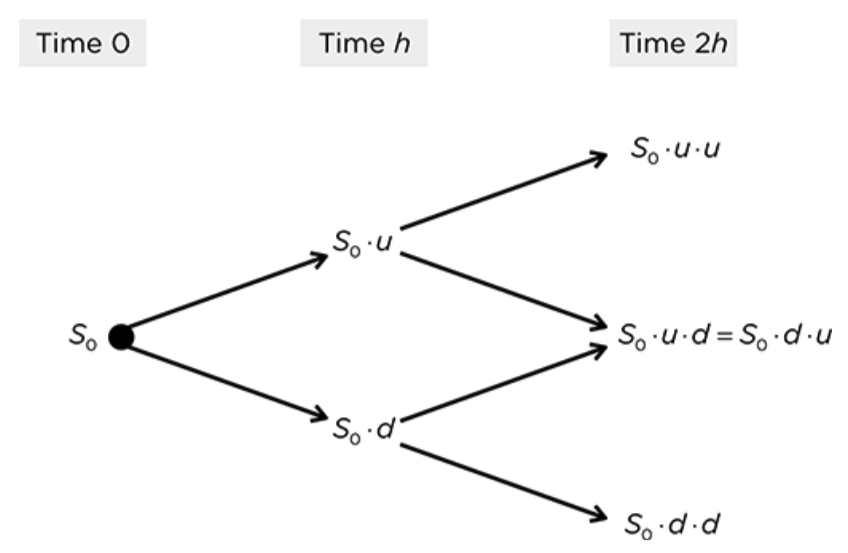
\includegraphics[scale=0.33]{../../src/ACT-2011/mult-per-bin-tree.png}
\end{center}

Lorsque les facteurs $u$ et $d$ sont fixes, l'arbre se recombine et $S_{0} \cdot u \cdot d = S_{0} \cdot d \cdot u$.

\subsubsection*{Évaluation neutre au risque}

Il y a 2 approches:
\begin{description}
	\item[Nœud par nœud]	On calcule la valeur de l'option à chaque nœud récursivement avec l'évaluation neutre au risque jusqu'à arriver au prix;
	\item[Approche directe]	Pour les \textbf{options européennes} dont l\textbf{'exercice hâtif n'est pas possible}.
\end{description}

\begin{algo2}[Approche directe]
\begin{enumerate}[leftmargin = *]
	\item	Calculer la valeur à l'échéance;
	\item	La pondérer par la probabilité neutre au risque de l'atteindre;
	\item	L'actualiser au taux sans risque.
\end{enumerate}
\tcbline
\begin{itemize}[leftmargin = *]
	\item	La probabilité d'atteindre un nœud terminal est calculée avec une distribution binomiale;
	\item	Pour $n$ périodes, $k$ est le nombre de hausses $u$ pour atteindre le nœud;
	\item	La probabilité est: \[\Pr(\text{atteindre un nœud ayant $k$ hausses})	=	\binom{n}{k} (p^{*})^{k} (1 - p^{*})^{n - k}\] pour $k = 0, 1, \dots, n$.
\end{itemize}
\end{algo2}

\begin{distributions}[Pour un nœud $u$]
\begin{align*}
	V_{u}	&=	\textrm{e}^{-r h}\left[ p^{*}V_{uu} + (1 - p^{*})V_{ud} \right]
\end{align*}
\end{distributions}

\subsubsection*{Portefeuille réplicatif}

$\Delta$ et $B$ ne restent pas constants et donc il faut prendre l'approche nœud par nœud. Ce faisant, il est \textit{\textbf{beaucoup}} plus compliqué et long de trouver le prix avec cette approche.

\begin{distributions}[Pour un nœud $u$]
\begin{align*}
	\Delta_{u}	&=	\textrm{e}^{-\delta h}\left( \frac{V_{uu} - V_{ud}}{S_{u}(u - d)} \right)	\\
	B_{u}	&=	\textrm{e}^{-r h} \left[ V_{ud}\left(	\frac{u}{u - d}\right) - V_{uu} \left(\frac{d}{u - d}\right) \right]	\\
	V_{u}	&=	\Delta_{u} S_{u} + B_{u}
\end{align*}
\end{distributions}

\columnbreak
\subsection{Tarification d'options américaines}
La distinction avec les options américaines est la possibilité d'un exercice hâtif.

\begin{description}
	\item[Valeur espérée actualisée (VEA)]	valeur (\og \textit{payoff} \fg{}) pour un maintien de l'option;
		\begin{itemize}[leftmargin = *]
		\item	\og \textit{Pull-back value}\fg{} car on se retire (\og \textit{pull-back} \fg{}) d'exercer l'option immédiatement.
		\end{itemize}
	\item[Valeur si levée (VSL)]	valeur (\og \textit{payoff} \fg{}) pour un exercice hâtif.
		\begin{itemize}[leftmargin = *]
		\item	\og \textit{Immediate exercice value} \fg{}.
		\end{itemize}
\end{description}

\begin{distributions}[Pour un nœud $u$]
\begin{align*}
VSL	&=	
	\begin{cases}
	\max(0, S_{u} - K),	&	\text{option d'achat}	\\
	\max(0, K - S_{u}),	&	\text{option de vente}
	\end{cases}
\end{align*}
\begin{align*}
	VEA	
	&=		\textrm{e}^{-r h}\left[ p^{*}V_{uu} + (1 - p^{*})V_{ud} \right]	\\
	V_{u}	
	&=	\max(VEA, VSL)
\end{align*}
\end{distributions}

\begin{algo2}[Processus de tarification]
\begin{enumerate}[leftmargin = *]
	\item	À partir du nœud le plus à droite de l'arbre décider à chaque nœud de l'arbre si l'exercice hâtif est optimal;
		\begin{itemize}[leftmargin = *]
		\item	Si $VSL > VEA$ alors il y a un exercice hâtif sinon on maintient l'option au moins une période de plus;
		\item	Donc $\text{valeur au nœud} = \max\left(\text{\shortstack{valeur pour un\\ maintien de l'option}}, \text{\shortstack{valeur pour un\\ exercice immédiat}}\right)$.
		\end{itemize}
	\item	Répéter jusqu'au nœud initial.
\end{enumerate}
\end{algo2}

\subsection{Tarification d'options sur un contrat à terme standardisé}
\textbf{Pas sur l'examen partiel hiver 2020.}

\begin{distributions}[Notation]
\begin{description}[leftmargin = *]
	\item[$T_{F}$]	temps d'expiration du contrat à terme standardisé;
	\item[$T$]	temps d'expiration d'une option;
		\begin{align*}
		T \le T_{F}
		\end{align*}
	\item[$F_{t, T_{F}}$]	Prix à terme au temps $t$ pour un contrat à terme standardisé expirant au temps $T_{F}$.
		\begin{align*}
		F_{t, T_{F}}
		&=	S_{t} \textrm{e}^{(r - \delta)(T_{F} - t)}
		\end{align*}
	\item[$u_{F}$ et $d_{F}$]	Facteurs de hausse et de baisse pour un arbre de contrats à terme standardisés;
		\begin{align*}
		u_{F}	
		&=	u \textrm{e}^{-(r - \delta)h}	=	\textrm{e}^{\sigma \sqrt{h}}	\\
		d_{F}
		&=	d \textrm{e}^{-(r - \delta)h}	=	\textrm{e}^{-\sigma \sqrt{h}}
		\end{align*}
\end{description}
\end{distributions}

L'équation pour un arbre de contrats à terme standardisés suffit de remplacer les paramètres:
\begin{align*}
	p^{*}	
		&=	\frac{\textrm{e}^{(r - \delta)h} - d}{u - d}	&
	&\Rightarrow	&
	p^{*}	
		&=	\frac{\textrm{e}^{(r -r)h} - d_{F}}{u_{F} - d_{F}}
		=	\frac{1 - d_{F}}{u_{F} - d_{F}}	\\
	u	
		&=	\textrm{e}^{(r - \delta)h + \sigma \sqrt{h}}	&
	&\Rightarrow	&
	u	
		&=	\textrm{e}^{(r - r)h + \sigma \sqrt{h}}	
		=	\textrm{e}^{\sigma \sqrt{h}}	\\
	d	
		&=	\textrm{e}^{(r - \delta)h - \sigma \sqrt{h}}	&
	&\Rightarrow	&
	d	
		&=	\textrm{e}^{(r - r)h - \sigma \sqrt{h}}	
		=	\textrm{e}^{-\sigma \sqrt{h}}	\\
	\Delta
		&=	\textrm{e}^{-\delta h} \left(\frac{V_{u} - V_{d}}{S(u - d)}\right)	&
	&\Rightarrow	&
	\Delta
		&=	\frac{V_{u} - V_{d}}{F(u_{F} - d_{F})}	\\
	B	
		&=	\textrm{e}^{-rh} \left[V_{d} \frac{u}{u - d} - V_{u}\frac{d}{u - d}\right]	&
	&\Rightarrow	&
	B
		&=	\textrm{e}^{-rh} [p^{*} V_{u} + (1 - p^{*}) V_{d}]
\end{align*}

\begin{align*}
	V_{u}
		&=	\Delta	(F u_{F} - F) + B \textrm{e}^{rh}	&
	V_{d}
		&=	\Delta	(F d_{F} - F) + B \textrm{e}^{rh}
\end{align*}

\subsection{Tarification d'options sur devises}
\begin{distributions}[Notation]
\begin{description}[leftmargin = *]
	\item[$r_{\text{DD}}$]	taux (force) d'intérêt sans risque sur le marché domestique;
	\item[$r_{\text{DÉ}}$]	taux (force) d'intérêt sans risque sur le marché étranger.
\end{description}
\end{distributions}

L'équation pour un arbre standard suffit de remplacer les paramètres:
\begin{align*}
	p^{*}	&=	\frac{\textrm{e}^{(r - \delta)h} - d}{u - d}	&
	&\Rightarrow	&
	p^{*}	&=	\frac{\textrm{e}^{(r_{\text{DD}} - r_{\text{DÉ}})h} - d}{u - d}	\\
	u	&=	\textrm{e}^{(r - \delta)h + \sigma \sqrt{h}}	&
	&\Rightarrow	&
	u	&=	\textrm{e}^{(r_{\text{DD}} - r_{\text{DÉ}})h + \sigma \sqrt{h}}	\\
	d	&=	\textrm{e}^{(r - \delta)h - \sigma \sqrt{h}}	&
	&\Rightarrow	&
	d	&=	\textrm{e}^{(r_{\text{DD}} - r_{\text{DÉ}})h - \sigma \sqrt{h}}	
\end{align*}
	
\subsection{Rendements composés continûment}
\begin{itemize}
	\item	La fonction \textbf{logarithmique} calcule des rendements composés continûment à partir des prix.
		\begin{align*}
		r_{t, t + h} &= \log\left(\frac{S_{t + h}}{S_{t}}\right)
		\end{align*}
	\item	La fonction \textbf{exponentielle} calcul des prix à partir des rendements composés continûment.
		\begin{align*}
		S_{t + h}	&=	S_{t}\textrm{e}^{r_{t, t + h}}
		\end{align*}
	\item	Les rendements composés continûment sont \textbf{additifs}.
		\begin{align*}
		r_{t, t + nh}	&=	\overset{n}{\underset{i = 1}{\sum}} r_{t + (i - 1)h, t + ih}
		\end{align*}
\end{itemize}	

	
\subsection{Volatilité}

\begin{distributions}[Notation]
\begin{description}[leftmargin = *]
	\item[$R$]	variable aléatoire de la force du rendement (sous base annuelle);
	\item[Hypothèse]	Les rendements composés continûment sur des périodes disjointes, mais de même longueur $h$, sont i.i.d.;
	\item[$r_{t, t + h}$]	le \textbf{rendement composé continûment entre $t$ et $t + h$}.
		\begin{align*}
		r_{t, t + h} &= \ln\left(\frac{S_{t + h}}{S_{t}}\right)
		\end{align*}
\end{description}
\end{distributions}

On suppose $n$ rendements, sur une période de $h$ années, composés continûment $r_{t, t + h}, r_{t + h, t + 2h}, \dots, r_{t + (n - 1)h, t + nh}$. \\
On peut estimer la volatilité historique avec:

\begin{align*}
	s_{h}
	&=	\sqrt{\frac{\overset{n}{\underset{i = 1}{\sum}} (r_{t + (i - 1)h, t + ih} - \bar{r})^{2}}{n - 1}}, &
	&\text{où}&
	\bar{r}
	&=	\frac{\overset{n}{\underset{i = 1}{\sum}} r_{t + (i - 1)h, t + ih}}{n}	&
\end{align*}

Donc $s_{h}$ estime $\sigma_{h}$ et $\bar{r}_{h}$ estime $\mu_{h}$ où:
	\begin{align*}
	\sigma_{h}
	&=	\sqrt{\text{Var}\left(\ln\left( \frac{S_{t + h}}{S_{t}} \right)\right)}	
	=	\sqrt{\text{Var}(R_{t, t + h})}	\\
	\mu_{h}
	&=	\text{E}[R_{t, t + h}]
	\end{align*}

Pour changer d'une base annuelle (le défaut de $h$) à une base quelconque, on divise par $h$ puisqu'il faut additionner $\frac{1}{h}$ rendements. \\
Par exemple, sous base mensuelle $h = \frac{1}{12}$ on a $\sigma = s_{1/12}\sqrt{12}$ ou sous base hebdomadaire $h = \frac{1}{52}$ on a $\sigma = s_{1/52}\sqrt{52}$.

\newpage

\section{Modèle binomial d’évaluation des options: sujets sélectionnés}

\subsection{Compréhension de l'exercice hâtif}

Avec un exercice hâtif, le détenteur d'une option {\color{amethyst}d'achat}:
\begin{enumerate}[leftmargin = *]
	\item	Reçoit l'action et donc les dividendes futurs.
		\begin{itemize}
		\item	Donc, on souhaite que $\delta$ \textcolor{amethyst}{augmente}.
		\end{itemize}
	\item	Paie le prix d'exercice avant expiration et donc subit des coûts d'intérêt.
		\begin{itemize}
		\item	Donc, on ne souhaite pas que $r$ \textcolor{amethyst}{augmente}.
		\end{itemize}
	\item	Perd l'assurance implicite à l'option.
		\begin{itemize}
		\item	Donc, on ne souhaite pas que $\sigma$ \textcolor{amethyst}{augmente}.
		\end{itemize}
\end{enumerate}

Le plus la volatilité $\sigma$ est élevée, le plus {\color{amethyst}élevé} {\color{burntsienna}(faible)} le prix de l'action auquel on va exercer l'option {\color{amethyst}d'achat} {\color{burntsienna}(de vente)}:
\begin{center}


\tikzset{every picture/.style={line width=0.75pt}} %set default line width to 0.75pt        

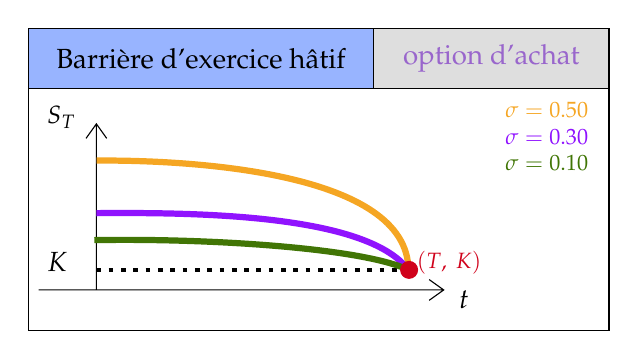
\begin{tikzpicture}[x=0.75pt,y=0.75pt,yscale=-1,xscale=1]
%uncomment if require: \path (0,225); %set diagram left start at 0, and has height of 225

%Straight Lines [id:da4209145739021405] 
\draw [line width=1.5]  [dash pattern={on 1.69pt off 2.76pt}]  (79.83,174.67) -- (230.5,174.67) ;
%Shape: Axis 2D [id:dp6241182322972705] 
\draw  (52,184.33) -- (247.17,184.33)(79.83,104.33) -- (79.83,184.33) (240.17,179.33) -- (247.17,184.33) -- (240.17,189.33) (74.83,111.33) -- (79.83,104.33) -- (84.83,111.33)  ;
%Curve Lines [id:da4521438515383944] 
\draw [color={rgb, 255:red, 245; green, 166; blue, 35 }  ,draw opacity=1 ][line width=2.25]    (80,122) .. controls (125.17,121.67) and (229.83,127.33) .. (230.17,174.67) ;
%Curve Lines [id:da48998708328548735] 
\draw [color={rgb, 255:red, 144; green, 19; blue, 254 }  ,draw opacity=1 ][line width=2.25]    (79.83,147.33) .. controls (125,147) and (209.83,147.33) .. (230.17,174.67) ;
%Curve Lines [id:da5987907161946171] 
\draw [color={rgb, 255:red, 65; green, 117; blue, 5 }  ,draw opacity=1 ][line width=2.25]    (78.83,160.33) .. controls (135.83,159.33) and (208.83,164.33) .. (230.17,174.67) ;
%Shape: Circle [id:dp3250882286176542] 
\draw  [draw opacity=0][fill={rgb, 255:red, 208; green, 2; blue, 27 }  ,fill opacity=1 ] (226.17,174.67) .. controls (226.17,172.27) and (228.11,170.33) .. (230.5,170.33) .. controls (232.89,170.33) and (234.83,172.27) .. (234.83,174.67) .. controls (234.83,177.06) and (232.89,179) .. (230.5,179) .. controls (228.11,179) and (226.17,177.06) .. (226.17,174.67) -- cycle ;

%Shape: Rectangle [id:dp47826177405826] 
\draw   (47,58.24) -- (326.83,58.24) -- (326.83,204) -- (47,204) -- cycle ;
%Shape: Rectangle [id:dp9903997496285197] 
\draw  [fill={rgb, 255:red, 152; green, 180; blue, 255 }  ,fill opacity=1 ] (47,58.33) -- (213.5,58.33) -- (213.5,87.13) -- (47,87.13) -- cycle ;
%Shape: Rectangle [id:dp7259398263822081] 
\draw  [fill={rgb, 255:red, 222; green, 222; blue, 222 }  ,fill opacity=1 ] (213.5,58.24) -- (326.83,58.24) -- (326.83,87.09) -- (213.5,87.09) -- cycle ;

% Text Node
\draw (130.25,72.73) node   [align=left] {Barrière d'exercice hâtif};
% Text Node
\draw (270.17,72.66) node   [align=left] {\color{amethyst}option d'achat};
% Text Node
\draw (269,91.33) node [anchor=north west][inner sep=0.75pt]  [font=\footnotesize] [align=left] {$\displaystyle  \begin{array}{{>{\displaystyle}l}}
\textcolor[rgb]{0.96,0.65,0.14}{\sigma =0.50}\\
\textcolor[rgb]{0.56,0.07,1}{\sigma =0.30}\\
\textcolor[rgb]{0.25,0.46,0.02}{\sigma =0.10}
\end{array}$};
% Text Node
\draw (257,189) node   [align=left] {$\displaystyle t$};
% Text Node
\draw (63,101) node  [font=\small] [align=left] {$\displaystyle S_{T}$};
% Text Node
\draw (61,171) node   [align=left] {$\displaystyle K$};
% Text Node
\draw (233,164.33) node [anchor=north west][inner sep=0.75pt]  [font=\footnotesize,color={rgb, 255:red, 208; green, 2; blue, 27 }  ,opacity=1 ] [align=left] {$\displaystyle ( T,\ K)$};


\end{tikzpicture}
\end{center}
\begin{center}
\tikzset{every picture/.style={line width=0.75pt}} %set default line width to 0.75pt        

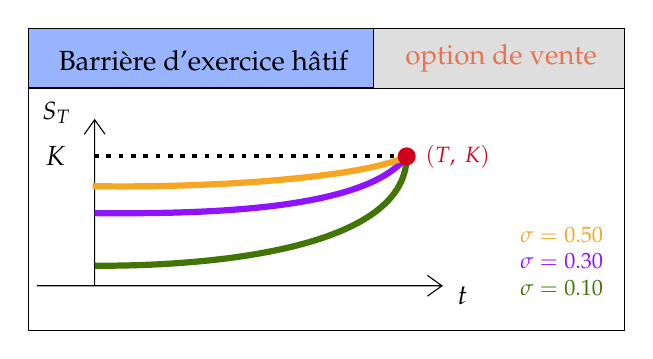
\begin{tikzpicture}[x=0.75pt,y=0.75pt,yscale=-1,xscale=1]
%uncomment if require: \path (0,225); %set diagram left start at 0, and has height of 225

%Straight Lines [id:da8257987800155955] 
\draw [line width=1.5]  [dash pattern={on 1.69pt off 2.76pt}]  (387.5,119.99) -- (538.17,119.99) ;
%Shape: Axis 2D [id:dp24873725999704033] 
\draw  (360,182.33) -- (555.17,182.33)(387.83,102.33) -- (387.83,182.33) (548.17,177.33) -- (555.17,182.33) -- (548.17,187.33) (382.83,109.33) -- (387.83,102.33) -- (392.83,109.33)  ;
%Curve Lines [id:da415072861376667] 
\draw [color={rgb, 255:red, 65; green, 117; blue, 5 }  ,draw opacity=1 ][line width=2.25]    (388,172.65) .. controls (433.17,172.99) and (537.83,167.32) .. (538.17,119.99) ;
%Curve Lines [id:da4265013005353009] 
\draw [color={rgb, 255:red, 144; green, 19; blue, 254 }  ,draw opacity=1 ][line width=2.25]    (387.83,147.32) .. controls (433,147.65) and (517.83,147.32) .. (538.17,119.99) ;
%Curve Lines [id:da4699510927961381] 
\draw [color={rgb, 255:red, 245; green, 166; blue, 35 }  ,draw opacity=1 ][line width=2.25]    (386.83,134.32) .. controls (443.83,135.32) and (516.83,130.32) .. (538.17,119.99) ;
%Shape: Circle [id:dp7867653202429181] 
\draw  [draw opacity=0][fill={rgb, 255:red, 208; green, 2; blue, 27 }  ,fill opacity=1 ] (533.83,119.99) .. controls (533.83,117.59) and (535.77,115.65) .. (538.17,115.65) .. controls (540.56,115.65) and (542.5,117.59) .. (542.5,119.99) .. controls (542.5,122.38) and (540.56,124.32) .. (538.17,124.32) .. controls (535.77,124.32) and (533.83,122.38) .. (533.83,119.99) -- cycle ;

%Shape: Rectangle [id:dp2982623700679301] 
\draw   (355.83,58.24) -- (642.92,58.24) -- (642.92,204) -- (355.83,204) -- cycle ;
%Shape: Rectangle [id:dp953868795068312] 
\draw  [fill={rgb, 255:red, 152; green, 180; blue, 255 }  ,fill opacity=1 ] (355.83,58.24) -- (522.33,58.24) -- (522.33,87.04) -- (355.83,87.04) -- cycle ;
%Shape: Rectangle [id:dp15029688089968674] 
\draw  [fill={rgb, 255:red, 222; green, 222; blue, 222 }  ,fill opacity=1 ] (522.33,58.24) -- (642.92,58.24) -- (642.92,87.09) -- (522.33,87.09) -- cycle ;

% Text Node
\draw (440.25,73.73) node   [align=left] {Barrière d'exercice hâtif};
% Text Node
\draw (583.67,72.66) node   [align=left] {\color{burntsienna}option de vente};
% Text Node
\draw (565,187) node   [align=left] {$\displaystyle t$};
% Text Node
\draw (371,99) node  [font=\small] [align=left] {\small $\displaystyle S_{T}$ };
% Text Node
\draw (369,120) node   [align=left] {$\displaystyle K$};
% Text Node
\draw (546,113.33) node [anchor=north west][inner sep=0.75pt]  [font=\footnotesize,color={rgb, 255:red, 208; green, 2; blue, 27 }  ,opacity=1 ] [align=left] {$\displaystyle ( T,\ K)$};
% Text Node
\draw (585,151.33) node [anchor=north west][inner sep=0.75pt]  [font=\footnotesize] [align=left] {$\displaystyle  \begin{array}{{>{\displaystyle}l}}
\textcolor[rgb]{0.96,0.65,0.14}{\sigma =0.50}\\
\textcolor[rgb]{0.56,0.07,1}{\sigma =0.30}\\
\textcolor[rgb]{0.25,0.46,0.02}{\sigma =0.10}
\end{array}$};


\end{tikzpicture}
\end{center}

Si la valeur de l'assurance est nulle (\lfbox[conditions]{$\sigma = 0$}) et que \lfbox[conditions]{$T \rightarrow \infty$}, on lève l'option {\color{amethyst}d'achat} si \lfbox[formula]{$\delta S_{T} {\color{amethyst}>} r K$}; c'est-à-dire, si la valeur des dividendes est {\color{amethyst}supérieure} à l'intérêt accumulé sur le prix d'exercice.\\

Pour une option de {\color{burntsienna}vente}, c'est {\color{burntsienna}l'inverse}.

\columnbreak
\subsection{Compréhension de l'évaluation neutre au risque}

\begin{distributions}[Notation]
\begin{itemize}[leftmargin = *]
	\item[$r$]	force d'intérêt sans risque;
	\item[$\delta$]	force de dividendes;
	\item[$\alpha$]	force d'intérêt (rendement) sur le sous-jacent;
	\item[$p$]	la vraie probabilité d'une hausse de l'actif sous-jacent;
		\begin{align*}
		p	&=	\frac{\textrm{e}^{(\alpha - \delta)h} - d}{u - d}
		\end{align*}
		\begin{itemize}
		\item	\lfbox[imphl]{on ne peut pas actualiser la valeur espérée de l'option avec $\alpha$ ni avec $r$};
		\item	L'option est risquée ce qui élimine $r$;
		\item	Le niveau de risque de l'option diffère de celui du sous-jacent.
		\end{itemize}
	\item[$\gamma$]	Force d'intérêt auquel on actualise la valeur espérée de l'option.
%	\item[]	$\alpha > r$ gain en capital + dividendes
%	\item[$p$]	vraie probabilité (que $S_{T}$ passe à $u^{*}S_{T}$).
\end{itemize}
Le prix est donc \lfbox[formula]{$V_{0}	=	\textrm{e}^{-\gamma h}(p V_{u} + (1 - p)V_{d})$}.
\end{distributions}

Pour un portefeuille réplicatif, $\textrm{e}^{\gamma h}	=	\left(	\frac{\Delta S}{\Delta S + B}\right)\textrm{e}^{\alpha h} + \left(\frac{B}{\Delta S + B}\right)\textrm{e}^{r h}$

\subsubsection*{Types de comportement envers le risque}
\begin{description}
	\item[Aversion au risque]	Souhaite maximiser le rendement espéré $\text{E}[R]$ tout en \textit{minimisant} le risque $\sigma^{2}_{R}$.
	\item[Indifférence au risque]	Souhaite maximiser le rendement espéré $\text{E}[R]$ et est \textit{indifférent} au risque $\sigma^{2}_{R}$.
		\begin{itemize}
		\item	On dit que l'investisseur est \textbf{\textit{neutre} au risque}.
		\end{itemize}
	\item[Exemple]	Soit 2 investissements: 1 000\$ assuré ou 2 000\$ avec une probabilité de 50\% et 0\$ avec une probabilité de 50\%.\\
					Un investisseur avec une \textit{aversion} au risque préfère la première option, car elle est moins risquée.	\\
					Un investisseur avec une \textit{indifférence} au risque est indifférent à la première ou la deuxième option, car le rendement espéré des deux options est égal.
\end{description}

Donc une évaluation neutre au risque suppose que les investisseurs sont indifférents au risque \textit{même s'ils ne le sont pas en réalité}.

%%%	------------------------------------
%%%	NOTE:
%%%	+	Pas couvert le bout sur \gamma puisque pas jugé nécessaire.
%%%	------------------------------------


\columnbreak
\subsection{L'arbre binomial et la lognormalité}
\subsubsection{Modèle de marche aléatoire}
\begin{distributions}[Notation]
\begin{description}
	\item[$Y_{i}$]	Variable aléatoire du $i^{\text{e}}$ résultat;
		\begin{itemize}
		\item	Si on lançait une pièce de monnaie, on aurait que $Y = -1$ si la pièce tombe sur pile et $Y	=	1$ si elle tombe sur face;
		\item	Également, $\Pr(Y	=	1)	=	\Pr(Y	=	-1)	=	\frac{1}{2}$;
		\item	$\text{E}[Y_{n}^{2}]	=	1$ et $\text{E}[Y_{n}]	=	0$;
		\end{itemize}
	\item[$Z_{n}$]	Total cumulatif après $n$ lancers.
		\begin{itemize}
		\item	$Z_{n}	=	\sumz{n}{i	=	1}Y_{i}$;
		\item	La magnitude $|Z_{n}|$ augmente avec $n$;
		\item	$\text{E}[Z_{n}^{2}]	=	n$ et $\text{E}[Z_{n}]	=	0$.
		\end{itemize}
\end{description}	
\end{distributions}

\textbf{Interprétation}:
\begin{itemize}
	\item	Dans un marché efficient, le prix devrait refléter toute l'information disponible. 		
	\item	Ainsi, par définition la nouvelle information est une surprise.
	\item	Le modèle de marche aléatoire pose que cette nouvelle information devrait résulter équiprobablement en une hausse ou une baisse du prix;
	\item	Après un certain temps, le prix d'une action dépend de l'effet cumulé de toutes les surprises.
\end{itemize}

\begin{conceptgen}{Problèmes avec la modélisation du prix de l'action}
Plusieurs problèmes nous empêchent d'utiliser une marche aléatoire:
\begin{enumerate}
	\item	Le prix de l'action \textbf{peut devenir négatif} s'il y a suffisamment de mouvements vers le bas. 
		\begin{itemize}
		\item	Ceci est impossible à cause de la responsabilité limitée des actionnaires \textit{(concept de GRF 1)}.
		\end{itemize}
	\item	La magnitude d'un mouvement ($|Y_{i}|$) est fixé à 1 mais devrait dépendre de: 
		\begin{enumerate}[label = \roman*)]
		\item	la \textbf{longueur} de la période $h$ (alias, la \textit{fréquence} des mouvements), et
		\item	le \textbf{prix actuel} $S_{t}$ de l'action sous-jacent.
		\end{enumerate}
		\begin{itemize}
		\item	Il n'est pas réaliste d'avoir le prix d'une action monter ou baisser de 60\$ en une journée.
		\end{itemize}
	\item	Le \textbf{rendement} sur l'action devrait, en moyenne, \textbf{être positif}.
\end{enumerate}
\end{conceptgen}

%%%	------------------------------------
%%%	NOTE
%%%	+	Pas couvert la distance carrée du point du départ qui est de n.
%%%	------------------------------------


Le modèle binomial est une variante du modèle de marche aléatoire qui résout ces problèmes; il suppose que les rendements composés continûment sont une \textbf{marche aléatoire avec dérive}. 

\subsubsection{Modèle binomial}

Selon le modèle binomial, \lfbox[formula]{$S_{t + h}	\in	S_{t}\textrm{e}^{(r	-	\delta)h \pm \sigma\sqrt{h}}$}.\\
Le rendement \lfbox[formula]{$r_{t, t + h}$}	$=	\ln\left(\frac{S_{t + h}}{S_{t}}\right)$	\lfbox[formula]{$\in	{\color{arsenic}(r	-	\delta)h} {\color{teal}\pm \sigma	\sqrt{h}}$} a donc 2 composantes: 
\begin{enumerate}
	\item	Une partie \textit{\textbf{certaine}} \lfbox[formula]{${\color{arsenic}(r	-	\delta)h}$},
		\begin{itemize}
		\item	Cette partie constitue \textit{la dérive}.
		\end{itemize}
	\item	Une partie \textit{\textbf{incertaine}} \lfbox[formula]{${\color{teal}\pm \sigma	\sqrt{h}}$}.
\end{enumerate}

On peut récrire le modèle binomiale comme:
\begin{align*}
	r_{t + (i - 1)h, t + ih}	
	&=	(r	-	\delta)h	+ Y_{i}\sigma	\sqrt{h}, \quad	i	=	1, 2, \dots, n	\\
	r_{0, nh}
	=	r_{0, T}
	&=	(r	-	\delta)T 	+ Z_{n}\sigma	\sqrt{h}
\end{align*}

Cette formulation du modèle règle donc les problèmes :
\begin{conceptgen}{Problèmes}
\begin{enumerate}[leftmargin = *]
	\item	Le \textbf{prix} de l'action \textbf{ne peut pas être négatif}.
	\item	La magnitude de la variation du prix dépend de la longueur de la période de temps $h$.
		\begin{itemize}
		\item	Des \textbf{mouvements} du prix de l'action \textbf{plus fréquents} diminuent $h$ et par conséquence la partie certaine du rendement ${\color{arsenic}(r	-	\delta)h}$.
		\end{itemize}
	\item	Le nouveau prix dépend du (est \textit{proportionnel} au) prix initial.
	\item	On peut garantir un \textbf{prix positif}. 
		\begin{itemize}[leftmargin = *]
		\item	Ceci, car il y a une composante certaine et que l'on choisit la probabilité d'une augmentation du prix.
		\end{itemize}
\end{enumerate}
\end{conceptgen}

\subsubsection{Lognormalité}

%%%	------------------------------------
%%%	NOTE
%%%	+	Pas couvert la probabilité de la i-ème node qui est une distribution binomial.
%%%	------------------------------------
L'arbre binomial est une approximation de la distribution lognormale.
\begin{itemize}
	\item	La somme de variables aléatoires binomiales est approximativement normalement distribuée;
	\item	Lorsque l'on traverse un arbre binomial, on somme implicitement les composantes du rendement;
	\item	Alors, lorsque le nombre de périodes \lfbox[conditions]{$n \rightarrow \infty$}, \lfbox[formula]{$r_{t, t + h}	\approx	\mathcal{N}\big((r	-	\delta)h, \sigma^{2}h\big)$};
	\item	Il s'ensuit que le prix $S_{t + T}	=$	\lfbox[formula]{$S_{t + nh}	\approx	\text{LN}$} lorsque \lfbox[conditions]{$n \rightarrow \infty$}.
\end{itemize}

On trouve alors que la probabilité d'atteindre le $(i + 1)^{\text{e}}$ nœud (à partir du haut) est:
\begin{align*}
	\Pr(S_{T}	=	S_{0}u^{n - i}d^{i})
	&=	\binom{n}{i} (p^{*})^{n - i}(1 - p^{*})^{i}, 	\quad	i	=	0, 1, \dots, n
\end{align*}

w\paragraph{Note}	Voir le chapitre \underline{\ref{sec:lognorm}: \nameref{sec:lognorm}} pour plus de détails sur l'application de la loi lognormale pour le prix d'actions.


\subsubsection{Arbres binomiaux alternatifs}
Il y existe d'autres façons de construire un arbre binomial qui mènent à des mouvements de $u$ et $d$ différents:

\begin{center}
\begin{tabular}{|	>{\columncolor{airforceblue}}c	| >{\columncolor{beaublue}}c | >{\columncolor{beaublue}}c  |}
\hline\rowcolor{airforceblue} 
\textcolor{white}{\textbf{Méthode}}	&	\textcolor{white}{\textbf{Mouvement} (u et d)}	&	\textcolor{white}{\textbf{Notes}}		\\\specialrule{0.1em}{0em}{0.0em} 
\textcolor{white}{Arbre à terme}		&	$\textrm{e}^{(r - \delta)h \pm \sigma \sqrt{h}}$	&	$u > \textrm{e}^{(r - \delta)h} > d$	\\\hline
\textcolor{white}{\shortstack{Arbre de\\ Cox-Ross-Rubenstein}}	&	$\textrm{e}^{\pm \sigma \sqrt{h}}$	&	$ud = 1$	\\\hline
\textcolor{white}{Arbre lognormal}	&	$\textrm{e}^{(r - \delta - \frac{1}{2}\sigma^{2})h \pm \sigma \sqrt{h}}$	&	$p^{*} \approx \frac{1}{2}$	\\\hline
\end{tabular}
\end{center}
\paragraph{Note}	Il est possible qu'avec un arbre de Cox-Ross-Rubenstein $\textrm{e}^{(r - \delta)h} > u$ si $h$ est gros et $\sigma$ petit.

\begin{itemize}
	\item	Malgré que toutes les différentes méthodes mènent à des prix différents lorsque $n$ est fini, elles tendent vers le même prix lorsque $n \rightarrow \infty$;
	\item	De plus, malgré que les mouvements $u$ et $d$ sont différents, le ratio des facteurs $\frac{u}{d}$ est le même:\\
		\begin{align*}
			\frac{u}{d}
			&=	\textrm{e}^{2\sigma\sqrt{h}}
		\end{align*}
	\item	Alors, peu importe la méthode utilisée pour construire l'arbre, la distance proportionnelle entre $u$ et $d$ mesure la volatilité.
\end{itemize} 

\columnbreak
\subsubsection*{Est-ce un modèle réaliste?}
Un modèle basé sur la distribution lognormale implique quelques hypothèses douteuses sur les prix qui, en pratique, ne sont pas vérifiées.

\begin{conceptgen}{Hypothèses douteuses d'une distribution normale}
\begin{enumerate}[label = \alph*), leftmargin = *]
	\item	Volatilité $\sigma$ constante.
		\begin{itemize}
		\item	En réalité, la volatilité change dans le temps.
		\end{itemize}
	\item	Pas de grandes variations spontanées.
		\begin{itemize}
		\item	En réalité, il y a parfois des chocs soudains des prix de titres boursiers.
		\end{itemize}
	\item	Indépendance entre les rendements composés continûment.
		\begin{itemize}
		\item	En réalité, les rendements sont positivement corrélés à court et moyen terme mais négativement corrélés à long terme.
		\end{itemize}
\end{enumerate}
\end{conceptgen}

Le modèle n'est donc pas parfait, mais sert plutôt de bon point de départ.

\newpage
\section{La formule de Black-Scholes}

\subsection{Formule de Black-Scholes généralisée}
\begin{conceptgen}{Hypothèses de la formule de Black-Scholes}
\begin{center}
	\textbf{Sur la distribution de l'action sous-jacente}
\end{center}
\begin{enumerate}[leftmargin = *, label = \alph*)]
	\item	Les rendements (composés continûment) sur l'action ont une distribution normale et sont indépendants à travers le temps.
	\item	La volatilité $\sigma$ des rendements (composés continûment) est connue et constante.
	\item	Les dividendes $\delta$ futurs sont connus.
\end{enumerate}
\tcbline
\begin{center}
	\textbf{Sur l'environnement économique}
\end{center}
\begin{enumerate}[leftmargin = *, label = \alph*)]
	\item	Le taux (force $r$) sans risque est connu et constant.
	\item	Il n'y a pas d'impôt	 ni de frais de transactions.
	\item	Il n'y a pas de frais de vente à découvert.
	\item	Les investisseurs peuvent emprunter au taux sans risque.
\end{enumerate}
\end{conceptgen}

Lorsque le nombre de périodes $n$ d'un arbre binomial augmente, le prix de l'option tend vers la valeur donnée par la formule de Black-Scholes.

\begin{definitionNOHFILL}[Formule de Black-Scholes généralisée]
Équations généralisées :

\begin{align*}
	d_{1}
	&=	\left(
			\frac{\ln\frac{F^{P}(S)}{F^{P}(K)} {\color{blue}{+}} \frac{1}{2} \sigma^{2} T}
	 			 {\sigma\sqrt{T}}
		\right)	&
	d_{2}
	&=	\left(
			\frac{\ln\frac{F^{P}(S)}{F^{P}(K)} {\color{red}{-}} \frac{1}{2} \sigma^{2} T}
	 			 {\sigma\sqrt{T}}
		\right)	
	=	d_{1} - \sigma \sqrt{t}	\\
\end{align*}

Prix d'options \textbf{européennes} selon la formule de Black-Scholes:

\begin{align*}
	C(S_{0}, K, \sigma, r, T, \delta)
	&=	F^{P}_{0, T}(S) N(d_{1}) - F^{P}_{0, T}(K) N(d_{2})	\\
	P(S_{0}, K, \sigma, r, T, \delta)
	&=	F^{P}_{0, T}(K) N(-d_{2}) - F^{P}_{0, T}(S) N(-d_{1})	
\end{align*}

\tcbline
\textbf{Notes}
\begin{align*}
	\sigma
	&=	\sqrt{\frac{\text{Var}(\ln F^{P}_{t, T}(S))}{t}}	
	=	\sqrt{\frac{\text{Var}(\ln F_{t, T}(S))}{t}}	
	=	\sqrt{\frac{\text{Var}(\ln S_{t})}{t}}, \, \forall 0 < t \le T	\\
\end{align*}

\begin{description}
	\item[$\ln S_{t}$]	\textbf{Volatilité de l'action} ou, de façon équivalente, volatilité du rendement sur l'action composé continûment.
\end{description}
\end{definitionNOHFILL}


\subsection{Options sur d'autres sous-jacents}

Avec la formule généralisée, on peut appliquer la formule de Black-Scholes à d'autres sous-jacents.\\ 
Dans un tel cas, il y a quelques considérations à prendre pour une option sur:
\begin{description}
	\item[Actions avec dividendes discrets proportionnels]	On trouve le nombre $n$ de fois que le dividende sera versé entre $0$ et l'échéance de $T$ de l'option.
		\begin{align*}
		F^{P}_{0, T}(S)
		&=	S_{0} (1 - txdiv)^{n}
		\end{align*}
	\item[Contrat à terme standardisé]	Il peut arriver que la date d'échéance---$T$---de l'option ne soit pas la même que la date d'échéance---$T'$---du contrat à terme standardisé sur un actif quelconque $Q$. \\
			Dans un tel cas, il faut que $T' \ge T$ et qu'on actualise le prix à terme $F_{0, T'}(Q)$ à partir de $T$ (et non $T'$).
			\begin{align*}
			F^{P}_{0, T}(F)	
			&=	F_{0, T'}(Q) \textrm{e}^{-rT}	&
			F^{P}_{0, T}(K)
			&=	K \textrm{e}^{-rT}	\\
			\end{align*}
	\item[Devises]	Les prix à terme prépayés doivent être dans la même devise que l'option.
		\begin{align*}
		C(S_{0} = x_{0}, K, \sigma, r = r_{\text{DD}}, T, \delta = r_{\text{DÉ}})
		&=	x_{0} \textrm{e}^{-r_{\text{DÉ}} T}N(d_{1}) - K \textrm{e}^{r_{\text{DD}}T} N(d_{2})	
		\end{align*}
\end{description}

%%%	-------------------------
%%%	NOTE
%%%	+	Ajouter clarification sur le K =/= nécessairment à F_{0, T'}(Q) et r =/= nécessairement \delta.
%%%	+	Compléter pour devises lorsque les notes de cours seront rendues disponibles.
%%%	-------------------------



\columnbreak

\subsection{Diagrammes du profit avant échéance}
Nous avons précédemment tracé des diagrammes de profit de valeur à l'échéance pour les options \textbf{à l'expiration}. Nous allons maintenant étendre ceci pour tracer les diagrammes \textbf{avant expiration}.
\begin{itemize}
	\item	L'idée est la même qu'auparavant mais on remplace la valeur à l'échéance par la valeur de revente de l'option
	\item	Pour tracer les diagrammes, on fait varier les prix en maintenant fixe les dates.
\end{itemize}

Nous illustrons ceci avec 2 stratégies:

\begin{definitionNOHFILL}[Achat et revente d'une option d'achat]
Crée en :
\begin{itemize}[leftmargin = *]
	\item	Achetant l'option d'achat au temps $t_{1}$;
	\item	Vendant l'option d'achat au temps $t_{2}$ avant l'échéance ($t_{2} < T$).
\end{itemize}

\begin{description}
	\item[Valeur à $t_{2}$]	
		\begin{align*}
		&=	\text{Prix de revente}	\\
		&=	C(S_{t_{2}}, K, \sigma, r, T, \delta)
		\end{align*}
	\item[Profit à $t_{2}$]	
		\begin{align*}
		&=	\text{Prix de revente} - \text{Prix d'achat à $t_{1}$ accumulé à $t_{2}$}	\\
		&=	C(S_{t_{2}}, K, \sigma, r, T, \delta) - C(S_{t_{1}}, K, \sigma, r, T, \delta) \textrm{e}^{r(t_{2} - t_{1})}
%%%		maybe mistake with T should be T  - t_{1}????
		\end{align*}
\end{description}
\end{definitionNOHFILL}

\begin{definitionNOHFILL}[Écart horizontal]
Crée en :
\begin{itemize}[leftmargin = *]
	\item	Vendant une option venant à échéance à $t_{1}$;
	\item	Achetant une option identique sauf pour la date d'échéance de $t_{2}$.
\end{itemize}

\begin{description}
	\item[Coût initial]	Pour des options d'achat on obtient:
		\begin{align*}
		&=	C(S, K, \sigma, r, T_{2}, \delta) - C(S, K, \sigma, r, T_{1}, \delta) 
		\end{align*}
\end{description}

\tcbline
%%%	--------------------
%%%	NOTE
%%%	+	Détailler davantage le contexte / profit / raisons pour
%%%	--------------------
\textbf{Notes}
\begin{itemize}[leftmargin = *]
	\item	Permet de spéculer sur la volatilité de l'action;
	\item	Typiquement utilisé lorsqu'un investisseur croit que, entre deux prix d'exercice, le prix va rester fixe;
	\item	L'écart est d'ailleurs bâtit afin d'avoir un thêta positif et implique la dissolution du portefeuille avant ou à la première des deux échéances;
	\item	en anglais \og \textit{calendar spread} \fg{}.
\end{itemize}
\end{definitionNOHFILL}

\subsection{Volatilité implicite}
\begin{description}
	\item[Volatilité implicite]	La valeur $\sigma$ tel que la formule de Black-Scholes reproduit le prix de l’option observé sur le marché.
\end{description}
\begin{itemize}[leftmargin = *]
	\item	La volatilité tel quel n'est pas observable et son estimation est problématique;
	\item	La volatilité \textit{historique} (vue au chapitre 10) n'est pas adéquate car elle ne prévoit pas le futur;
	\item	On peut en lieu isoler la volatilité \textit{implicite} $\hat{\sigma}$ avec le prix observé de l'action et la formule de Black-Scholes.	\\
			Elle représente donc l'appréciation de la volatilité faite par le marché;
	\item	Malgré que la volatilité est supposée constante dans la formule, en réalité elle varie selon le prix d'exercice $K$ et la date d'échéance $T$;
	\item	On peut l'utiliser pour évaluer une option qui n'existe pas encore;
	\item	Également, on peut valider ou invalider le modèle de Black-Scholes;
	\item	Finalement, on peut comparer des options par leur volatilité implicite au lieu de leurs prix.
%	\item	En voyant le marché des options comme un marché qui transige la volatilité, on peut la révéler.\\
%			Selon cette théorie, les prix d'options révèlent les attentes du marché de la distribution des prix d'actions dans le futur.
\end{itemize}

\newpage


\section*{Les Grecs de l'option}
\addcontentsline{toc}{section}{Les Grecs de l'option}
Les grecs servent à mesurer l'exposition au risque en considérant un paramètre de la formule de Black-Scholes à la fois.
\begin{itemize}
	\item	Par défaut, on calcule les grecs en supposant l'achat (et non la vente) d'une option.
\end{itemize}

\begin{center}
\begin{tabular}{|	>{\columncolor{airforceblue}}c	| >{\columncolor{beaublue}}c | >{\columncolor{beaublue}}m{0.5\columnwidth}  |}
\hline\rowcolor{airforceblue} 
\textcolor{white}{\textbf{Grec}}	&	\textcolor{white}{\textbf{Définition}}	&	\textcolor{white}{\textbf{Mesure le changement de la valeur ($V$)}}		\\\specialrule{0.1em}{0em}{0.0em} 
$\Delta$	&	$\deriv{S_{0}}{V}$	&	de l'option par une augmentation (de 1\$) du prix de l'action.	\\
$\Gamma$	&	$\deriv{S_{0}}{\Delta} = \deriv[2]{S_{0}}{V}$	&	du Delta par une augmentation (de 1\$) du prix de l'action.	\\
$\theta/365$	&	$\deriv{t}{V}$	&	de l'option par une baisse (d'un jour) de la date d'échéance.	\\
\textbf{Vega}	&	$\deriv{\sigma}{V}$	&	de l'option par une augmentation (de 1\%) de la volatilité.	\\
$\rho/100$	&	$\deriv{r}{V}$	&	de l'option par une augmentation (de 1\%) du taux sans risque.	\\
$\psi/100$	&	$\deriv{\delta}{V}$	&	de l'option par une augmentation (de 1\%) de la force de dividende.	\\
\end{tabular}
\end{center}

\begin{distributions}[Termes financiers]
\begin{description}
	\item[point de pourcentage]	$1\%$.
	\item[point de base]	$0.01\%$.
\end{description}
\end{distributions}

\columnbreak

\subsection{Grecs}

\begin{definitionNOHFILL}[Delta $\Delta	=	\deriv{S_{0}}{V}$]
Mesure la variation du prix de l'option correspondante à une augmentation du prix de l'action.

\tcbline

\begin{minipage}[ht]{0.5\linewidth}
\begin{center}
	\textbf{Expressions du Delta pour les options}
\end{center}
\begin{gather}
\begin{align*}
	\Delta_{C}
	&=	\textrm{e}^{-\delta T} N(d_{1})	\\
	\Delta_{P}
	&=	-\textrm{e}^{-\delta T} N(-d_{1})	
\end{align*}
\end{gather}
\end{minipage}
\begin{minipage}[ht]{0.5\linewidth}
\begin{center}
	\textbf{Domaine}
\end{center}
\begin{gather}
\begin{align*}
	0 \le \Delta_{C} \le 1	\\
	-1 \le \Delta_{P} \le 0	
\end{align*}
\end{gather}
\end{minipage}

\tcbline
Lien entre le delta pour une options de vente et d'achat:
\begin{align*}
%	C - P	&=	S\textrm{e}^{-\delta T} - K\textrm{e}^{-rT}	\\
%	\deriv{S}{C} - \deriv{S}{P}	&=	\deriv{S}{} (S\textrm{e}^{-\delta T}) - \deriv{S}{} (K\textrm{e}^{-rT})	\\
	\Delta_{C} - \Delta_{P}	&=	\textrm{e}^{-\delta T}
\end{align*}

\begin{center}
	\textbf{Notes}
\end{center}
\begin{itemize}[leftmargin = *]
	\item	Le Delta $\Delta_{C}$ ($\Delta_{P}$) peut être interprété comme le nombre d'actions à acheter (vendre) pour répliquer une option d'achat (de vente);
	\item	Une option d'achat devient de plus en plus profitable lorsque le prix de l'action sous-jacente augmente. \\
			Alors, $\Delta_{C}$ se rapproche de 0 lorsque l'option est hors du cours ($S_{T} < K$) et de 1 lorsqu'elle est dans le cours ($S_{T} > K$).\\
			Cependant, le $\Delta_{C}$ ne sera jamais négatif, car l'option d'achat a un seuil minimal de 0 pour sa valeur à l'échéance.\\
			De même, $\Delta_{P}$ ne sera jamais positif;
	\item	Dans les deux cas, le $\Delta$ augmente avec le prix de l'action;
	\item	Mathématiquement, le domaine est restreint puisque $0 \le N(x) \le 1, \forall x$ et $0 \le e^{-\delta T} \le 1$.
\end{itemize}
\end{definitionNOHFILL}

\begin{definitionNOHFILL}[Gamma $\Gamma = \deriv{S_{0}}{\Delta} = \deriv[2]{S_{0}}{V}$]
Mesure la variation du Delta de l'option correspondante à une augmentation du prix de l'action.

\tcbline

\begin{minipage}[ht]{0.5\linewidth}
\begin{center}
	\textbf{Expressions du Gamma pour les options}
\end{center}
\begin{gather}
\begin{align*}
	\Gamma_{C}
	&=	\Gamma_{P}
	=	\frac{\textrm{e}^{-\delta T} N'(d_{1})}{S_{0} \sigma \sqrt{T}}	
\end{align*}
\end{gather}
\end{minipage}
\begin{minipage}[ht]{0.5\linewidth}
\begin{center}
	\textbf{Domaine}
\end{center}
\begin{gather}
\begin{align*}
	\Gamma_{P}	=	\Gamma_{C}	>	0
\end{align*}
\end{gather}
\end{minipage}

\tcbline

\begin{center}
	\textbf{Notes}
\end{center}
\begin{itemize}[leftmargin = *]
	\item	Le $\Gamma$ mesure le \textit{taux} de variation du $\Delta$.\\
			Puisque le $\Delta$ augmente toujours, le $\Gamma$ est toujours positif;
	\item	Le $\Gamma$ est maximisé au cours du marché, car c'est où le $\Delta$ connaît le plus de variation.
		\begin{center}
		

\tikzset{every picture/.style={line width=0.75pt}} %set default line width to 0.75pt        

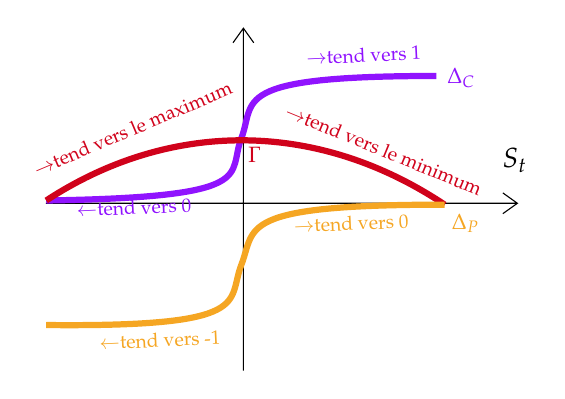
\begin{tikzpicture}[x=0.75pt,y=0.75pt,yscale=-1,xscale=1]
%uncomment if require: \path (0,225); %set diagram left start at 0, and has height of 225

%Shape: Axis 2D [id:dp24873725999704033] 
\draw  (71,130.67) -- (298.17,130.67)(166.17,46.33) -- (166.17,211.33) (291.17,125.67) -- (298.17,130.67) -- (291.17,135.67) (161.17,53.33) -- (166.17,46.33) -- (171.17,53.33)  ;
%Curve Lines [id:da415072861376667] 
\draw [color={rgb, 255:red, 144; green, 19; blue, 254 }  ,draw opacity=1 ][line width=2.25]    (71.17,129.33) .. controls (175.17,127.67) and (158.17,117.33) .. (165.17,99.33) .. controls (172.17,81.33) and (158.17,69.33) .. (259.17,69.33) ;
%Curve Lines [id:da4699510927961381] 
\draw [color={rgb, 255:red, 208; green, 2; blue, 27 }  ,draw opacity=1 ][line width=2.25]    (71.17,129.33) .. controls (129.17,91.33) and (200.17,89.33) .. (263.17,131.33) ;
%Curve Lines [id:da7102609332275407] 
\draw [color={rgb, 255:red, 245; green, 166; blue, 35 }  ,draw opacity=1 ][line width=2.25]    (71.17,189.33) .. controls (172.17,190.33) and (158.17,178.33) .. (165.17,160.33) .. controls (172.17,142.33) and (162.17,131.33) .. (263.17,131.33) ;

% Text Node
\draw (297,110) node   [align=left] {$\displaystyle S_{t}$};
% Text Node
\draw (263,64.33) node [anchor=north west][inner sep=0.75pt]  [font=\footnotesize,color={rgb, 255:red, 144; green, 19; blue, 254 }  ,opacity=1 ] [align=left] {$\displaystyle \Delta _{C}$};
% Text Node
\draw (265.17,134.33) node [anchor=north west][inner sep=0.75pt]  [font=\footnotesize,color={rgb, 255:red, 245; green, 166; blue, 35 }  ,opacity=1 ] [align=left] {$\displaystyle \Delta _{P}$};
% Text Node
\draw (167.17,102.33) node [anchor=north west][inner sep=0.75pt]  [font=\footnotesize,color={rgb, 255:red, 208; green, 2; blue, 27 }  ,opacity=1 ] [align=left] {$\displaystyle \Gamma $};
% Text Node
\draw (62.5,110.69) node [anchor=north west][inner sep=0.75pt]  [font=\scriptsize,rotate=-337.11] [align=left] {\textcolor[rgb]{0.82,0.01,0.11}{$\displaystyle \rightarrow ${\scriptsize tend vers le maximum}}};
% Text Node
\draw (187.55,80.84) node [anchor=north west][inner sep=0.75pt]  [font=\scriptsize,rotate=-22.32] [align=left] {\textcolor[rgb]{0.82,0.01,0.11}{$\displaystyle \rightarrow $}{\scriptsize \textcolor[rgb]{0.82,0.01,0.11}{tend vers le minimum}}};
% Text Node
\draw (194.96,55.91) node [anchor=north west][inner sep=0.75pt]  [font=\scriptsize,color={rgb, 255:red, 144; green, 19; blue, 254 }  ,opacity=1 ,rotate=-357.41] [align=left] {\textcolor[rgb]{0.56,0.07,1}{$\displaystyle \rightarrow ${\scriptsize tend vers 1}}};
% Text Node
\draw (84.3,129.24) node [anchor=north west][inner sep=0.75pt]  [font=\scriptsize,color={rgb, 255:red, 144; green, 19; blue, 254 }  ,opacity=1 ,rotate=-357.41] [align=left] {\textcolor[rgb]{0.56,0.07,1}{$\displaystyle \leftarrow $}{\scriptsize \textcolor[rgb]{0.56,0.07,1}{tend vers 0}}};
% Text Node
\draw (95.3,193.24) node [anchor=north west][inner sep=0.75pt]  [font=\scriptsize,color={rgb, 255:red, 144; green, 19; blue, 254 }  ,opacity=1 ,rotate=-357.41] [align=left] {\textcolor[rgb]{0.96,0.65,0.14}{$\displaystyle \leftarrow ${\scriptsize tend vers -1}}};
% Text Node
\draw (188.96,136.91) node [anchor=north west][inner sep=0.75pt]  [font=\scriptsize,color={rgb, 255:red, 144; green, 19; blue, 254 }  ,opacity=1 ,rotate=-357.41] [align=left] {\textcolor[rgb]{0.96,0.65,0.14}{$\displaystyle \rightarrow ${\scriptsize tend vers 0}}};


\end{tikzpicture}
		\end{center}
\end{itemize}
\end{definitionNOHFILL}

\begin{definitionNOHFILL}[Theta $\theta	=	\deriv{t}{V}$]
Mesure la variation du prix de l'option correspondante à l'écoulement du temps.

\paragraph{Note}	Selon si on dérive par rapport au point de départ $t$ ou à l'échéance $T$ on a que \icbox[red][palechestnut]{$\theta	=	\deriv{t}{V}	=	-\deriv{T}{V}$}

\tcbline
Lien entre le delta pour une options de vente et d'achat:
\begin{align*}
	\theta_{C} - \theta_{P}	&=	\delta S \textrm{e}^{-\delta (T - t)}	-	r K \textrm{e}^{-r (T - t)}
\end{align*}

\begin{center}
	\textbf{Expressions du Theta pour les options}
\end{center}
	\setlength{\mathindent}{0cm}
\begin{gather}
\begin{align*}
	\theta_{C}
	&=	\left(S_{0}\delta \textrm{e}^{-\delta (T - t)} N(d_{1})	-	Kr \textrm{e}^{-r (T - t)} N(d_{2})\right) -
		\frac{K\textrm{e}^{-r (T - t)} N'(d_{2}) \sigma}{2\sqrt{T - t}}	\\
	\theta_{P}
	&=	\left(Kr \textrm{e}^{-r (T - t)} N(-d_{2})	-	S_{0}\delta \textrm{e}^{-\delta (T - t)} N(-d_{1})\right) -
		\frac{K\textrm{e}^{-r (T - t)} N'(d_{2}) \sigma}{2\sqrt{T - t}}	\\
\end{align*}
	\setlength{\mathindent}{1cm}
\end{gather}

\tcbline

\begin{center}
	\textbf{Notes}
\end{center}
\begin{itemize}[leftmargin = *]
	\item	Pour obtenir la variation en valeur par jour---\textbf{la notation de Claire}---il suffit de diviser par 365: \icbox{$\frac{\theta}{365}$};
	\item	La valeur d'une option décroît avec le temps. \\
			$\theta$ estime de combien, ceteris paribus, la valeur décroît par jour;
	\item	Ce faisant, $\theta$ est habituellement \textbf{négatif}.\\
			Il est \textit{possible} qu'il soit positif pour une option \underline{profondément} dans le cours du marché ayant un taux de dividende \underline{très} élevé;
	\item	\textbf{T}heta pour \textbf{t}emps.
\end{itemize}
\end{definitionNOHFILL}

\begin{definitionNOHFILL}[Vega alias Lambda $\Lambda	=	\deriv{\sigma}{V}$]
Mesure la variation du prix de l'option correspondante à une augmentation de la volatilité de l'action.
\tcbline

\begin{minipage}[ht]{0.5\linewidth}
\begin{center}
	\textbf{Expression du Vega pour les options}
\end{center}
\begin{gather}
\begin{align*}
	\Lambda_{C}
	&=	\Lambda_{P}
	=	S_{0} \textrm{e}^{-\delta T} N'(d_{1}) \sqrt{T}
\end{align*}
\end{gather}
\end{minipage}
\begin{minipage}[ht]{0.5\linewidth}
\begin{center}
	\textbf{Domaine}
\end{center}
\begin{gather}
\begin{align*}
	\Lambda_{P}	=	\Lambda_{C}	>	0
\end{align*}
\end{gather}
\end{minipage}

\tcbline

\begin{center}
	\textbf{Notes}
\end{center}
\begin{itemize}[leftmargin = *]
	\item	Pour obtenir la variation en pourcentage---\textbf{la notation de Claire}---il suffit de diviser par 100: \icbox{$\frac{\Lambda}{100}$};
	\item	Une augmentation de la volatilité mène toujours à une augmentation des prix d'options.\\
			Il s'ensuit que le Vega sera toujours positif et augmente avec la volatilité;
	\item	\textbf{V}ega pour \textbf{v}olatilité.
\end{itemize}
\end{definitionNOHFILL}

\begin{definitionNOHFILL}[Rho $\rho	=	\deriv{r}{V}$]
Mesure la variation du prix de l'option correspondante à une augmentation du taux sans risque.

\tcbline

\begin{minipage}[ht]{0.5\linewidth}
\begin{center}
	\textbf{Expression du Rho pour les options}
\end{center}
\begin{gather}
\begin{align*}
	\rho_{C}
	&=	T K \textrm{e}^{-r T} N(d_{2})	\\
	\rho_{P}
	&=	-T K \textrm{e}^{-r T} N(-d_{2})
\end{align*}
\end{gather}
\end{minipage}
\begin{minipage}[ht]{0.5\linewidth}
\begin{center}
	\textbf{Domaine}
\end{center}
\begin{gather}
\begin{align*}
	\rho_{C}	&>	0	\\
	\rho_{P}	&<	0
\end{align*}
\end{gather}
\end{minipage}


\tcbline

\begin{center}
	\textbf{Notes}
\end{center}
\begin{itemize}[leftmargin = *]
	\item	Pour obtenir la variation en pourcentage---\textbf{la notation de Claire}---il suffit de diviser par 100: \icbox{$\frac{\rho}{100}$};
	\item	Une augmentation du taux sans risque $r$ fait baisser la valeur actualisée du prix d'exercice $K\textrm{e}^{-rT}$.\\
			Selon la formule de Black-Scholes, baisser $K\textrm{e}^{-rT}$ fait \textbf{augmenter} la valeur d'une option d'achat mais \textbf{baisser} celle d'une option de vente.\\
			Donc, $\rho_{C} > 0$ et $\rho_{P} < 0$;
	\item	\textbf{R}ho pour taux sans \textbf{r}isque.
\end{itemize}
\end{definitionNOHFILL}

\begin{definitionNOHFILL}[Psi $\psi	=	\deriv{\delta}{V}$]
Mesure la variation du prix de l'option correspondante à une augmentation du taux de dividendes.

\tcbline


\begin{minipage}[ht]{0.5\linewidth}
\begin{center}
	\textbf{Expression du Psi pour les options}
\end{center}
\begin{gather}
\begin{align*}
	\psi_{C}
	&=	- T S \textrm{e}^{-\delta T} N(d_{1})	\\
	\psi_{P}
	&=	T S \textrm{e}^{-\delta T} N(-d_{1})
\end{align*}
\end{gather}
\end{minipage}
\begin{minipage}[ht]{0.5\linewidth}
\begin{center}
	\textbf{Domaine}
\end{center}
\begin{gather}
\begin{align*}
	\psi_{C}	&<	0	\\
	\psi_{P}	&>	0
\end{align*}
\end{gather}
\end{minipage}

\tcbline

\begin{center}
	\textbf{Notes}
\end{center}
\begin{itemize}[leftmargin = *]
	\item	Pour obtenir la variation en pourcentage---\textbf{la notation de Claire}---il suffit de diviser par 100: \icbox{$\frac{\psi}{100}$};
	\item	Une augmentation du taux de dividendes $\delta$ fait baisser la valeur actualisée du prix de l'action $S\textrm{e}^{-\delta T}$.\\
			Selon la formule de Black-Scholes, baisser $S\textrm{e}^{-\delta T}$ fait \textbf{baisser} la valeur d'une option d'achat mais \textbf{augmenter} celle d'une option de vente.\\
			Donc, $\psi_{C} < 0$ et $\psi_{P} > 0$.
\end{itemize}
\end{definitionNOHFILL}

\subsubsection*{Portefeuille}

Le grec d'un portefeuille composé de $N$ options sur une même action, avec $n_{i}$ options de chaque type, est simplement la somme des grecques:
\begin{align*}
	\text{Grec}_{\text{ptf.}}
	&=	\overset{N}{\underset{i = 1}{\sum}} n_{i} \text{Grec}_{i}	
\end{align*}

\columnbreak

\subsection{Élasticité}


\begin{definitionNOHFILL}[Élasticité $\Omega	=	\frac{\Delta S_{0}}{V}$]
Mesure le pourcentage de variation du prix de l'option correspondante au pourcentage d'augmentation du prix de l'action.

\tcbline

\begin{center}
	\textbf{Élasticité}
\end{center}
\begin{align*}
		\Omega_{\text{option}}
		&=	\frac{\text{\% variation du prix de l'option}}{\text{\% variation du prix de l'action}}	
		=	\frac{{\color{teal}(V_{t} - V_{0})}/V_{0}}{{\color{teal}(S_{t} - S_{0})}/S_{0}}	\\
		&=	{\color{teal}\Delta} \cdot \frac{S_{0}}{V_{0}}
		=	\frac{\Delta S_{0}}{V}
\end{align*}

\begin{center}
	\textbf{Bornes}
\end{center}
\begin{gather}
\begin{align*}
	\Omega_{C}	&\ge		1	&
	\Omega_{P}	&\le		0
\end{align*}
\end{gather}

\tcbline

\begin{center}
	\textbf{Notes}
\end{center}
\begin{itemize}[leftmargin = *]
	\item	Pour obtenir la variation par augmentation de 1\% du prix de l'action---\textbf{la notation de Claire}---il suffit de diviser par 100: \icbox{$\frac{\Omega}{100}$};
	\item	Le $\Delta$ peut être vu comme le risque \textit{absolu} d'une action: \[\Delta = \frac{\text{variation du prix de l'option}}{\text{variation du prix de l'action}}\]
			L'élasticité évalue plutôt le risque \textit{relatif} au montant.
\end{itemize}
\end{definitionNOHFILL}

\subsubsection*{Volatilité}
Puisqu'un actif sans risque n'a aucune volatilité, la volatilité de l'option ($\sigma_{\text{option}}$) va seulement dépendre de celle de l'action ($\sigma_{\text{action}}$).\\
On ne fait que pondérer par la valeur absolue de l'élasticité de l'option ($\Omega_{\text{option}}$): \lfbox[formula]{$\sigma_{\text{option}}
	=	\left| \Omega_{\text{option}} \right| \sigma_{\text{action}}$}.
%\begin{align*}
%	
%\end{align*}

\begin{itemize}
	\item	La valeur absolue assure une volatilité positive.
\end{itemize}

\subsubsection*{Rendement sur l'option $\gamma$}
Pour un portefeuille réplicatif on a que $V = \Delta S + B$. \\
Avec ceci on trouve:
\begin{description}
	\item[\% investit dans l'action sous-jacente]	$\% \text{ action} = \frac{\Delta S}{V} = \Omega$.
	\item[\% investit dans l'actif sans risque]	$\% \text{ actif} = \frac{B}{V} = 1 - \Omega$.
	\item[$\gamma$]	Rendement espéré instantané sur l'option.
		\begin{itemize}
		\item	On pondère les rendements sur l'action et l'actif:	
		\end{itemize}
		\begin{align*}
		\gamma 
		&=	(\% \text{ action}) \alpha + (\% \text{ actif}) r	\\
		&=	\Omega \alpha + (1 - \Omega) r
		\end{align*}
\end{description}
\begin{itemize}[leftmargin = *]
	\item	Ceci est l'équivalent continu de $\textrm{e}^{\gamma h} = \frac{\delta S}{\delta S + B}\textrm{e}^{\alpha h} + \frac{B}{\delta S + B}\textrm{e}^{r h}$.
\end{itemize}

\begin{definitionNOHFILLsub}[Prime de risque]
Une \textbf{prime de risque} est l'excès du rendement espéré d'un actif au taux sans risque.
\begin{description}
	\item[Prime de risque sur l'action]	$\alpha - r$
	\item[Prime de risque sur l'option]	$\gamma - r$
\end{description}
\begin{itemize}[leftmargin = *]
	\item	Avec la définition du rendement $\gamma$ espéré instantané sur l'option on trouve: \icbox{$	\gamma - r = \Omega (\alpha - r)$};
	\item	Dans le modèle d'évaluation des actifs financiers, \icbox{$\alpha - r = \beta_{\text{action}}(\mu_{m} - r)$} alias $\beta_{\text{option}}	=	\beta_{\text{action}} \Omega_{\text{option}}$;
	\item	Si $\alpha > r$ alors $\gamma_{C} \geq \alpha$ et $\gamma_{P} \leq r$.
\end{itemize}
\end{definitionNOHFILLsub}

\begin{definitionNOHFILL}[Ratio de Sharpe \o]
Le \textbf{ratio de Sharpe} d'un actif est le ratio de sa prime de risque à sa volatilité.
\begin{description}
	\item[Ratio de Sharpe de l'action]	
		\begin{align*}
		\text{\o}_{\text{action}}	
		&=	\frac{\alpha - r}{\sigma_{\text{action}}}
		\end{align*}
	\item[Ratio de Sharpe de l'option]	
		\begin{align*}
		\text{\o}_{\text{option}}	
		&=	\frac{\gamma - r}{\sigma_{\text{option}}}	
		=	\frac{\Omega (\alpha - r)}{|\Omega|\sigma_{\text{action}}}	
		\end{align*}
\end{description}
Puisque $\Omega$ est positif pour les options d'achat et négatif pour les options de vente:
\begin{align*}
	\text{\o}_{C}	&=	\text{\o}_{\text{action}}	&
	\text{\o}_{P}	&=	-\text{\o}_{\text{action}}
\end{align*}
\end{definitionNOHFILL}

\subsubsection*{Portefeuille}

L'élasticité d'un portefeuille composé de $N$ options avec $n_{i}$ de chaque type est la moyenne pondérée de l'élasticité de chaque type d'option.\\
Donc, avec $\omega_{i}$\% du portefeuille investi dans l'option $i$, on a:
\begin{align*}
	\Omega_{\text{ptf.}}
	&=	\overset{N}{\underset{i = 1}{\sum}} \omega_{i} \Omega_{i}, \: \text{où } \omega_{i} = n_{i} \times \frac{V_{i}}{V_{\text{ptf.}}}
\end{align*}

On peut également le calculer avec les paramètres du portefeuille $\Omega_{\text{ptf.}} = \frac{\Delta_{\text{ptf.}}S}{V_{\text{ptf.}}}$.

\subsection{Approximation}

\begin{itemize}[leftmargin = *]
	\item	On peut approximer la variation du prix de l'option avec les grecques;
	\item	Le Delta \textit{varie avec le prix}: 
		\begin{itemize}
		\item	Le Delta \textit{sous-estime} l'\textit{augmentation} du prix de l'option d'achat quand le prix de l'action augmente et \textit{surestime} la \textit{diminution};
		\item	Alors, le Delta est seulement valide comme approximation du prix pour des très petites variations
		\end{itemize}
	\item	En considérant le Gamma, l'approximation devient valide pour des plus grandes variations;
	\item	Cependant, la meilleure approximation se fait en incluant Theta pour considérer \textit{l'effet du temps}.
\end{itemize}

\begin{definitionNOHFILL}[Approximation Delta-Gamma-Theta]
\begin{align*}
	C(S_{t} + \varepsilon)
	&\approx	C(S_{t}) + \Delta_{t} \varepsilon + \frac{1}{2} \Gamma_{t} \varepsilon^{2} + \theta_{t} h
\end{align*}

\tcbline

\textbf{Notes}
\begin{itemize}[leftmargin = *]
	\item	$\varepsilon$ est la variation du prix.
	\item	$h$ et $\theta$ doivent être dans la même unité de temps.
	\item	$\theta$ diminue l'approximation, car il est habituellement négatif.
\end{itemize}
\end{definitionNOHFILL}

%Pour un nœud $\eta$, on va avoir:
%\begin{align*}
%	(\Delta_{\eta u} - \Delta_{\eta})S_{\eta u} + (B_{\eta u} - B_{\eta}\textrm{e}^{rh})	\\
%	(\Delta_{\eta d} - \Delta_{\eta})S_{\eta d} + (B_{\eta d} - B_{\eta}\textrm{e}^{rh})
%\end{align*}

\newpage

\section{Tenue de marché et couverture en delta neutre}

\begin{definitionNOHFILL}[Opérations pour compte propre]
Opérations effectuées par une institution financière pour son propre compte afin de suivre une stratégie d'investissement.

\begin{itemize}[leftmargin = *]
\item	En anglais \og \textit{proprietary trading} \fg{};
\item	On distingue les opérations pour compte propre de la tenue de marché:
	\begin{itemize}[leftmargin = *]
	\item	Les clients et opérateurs pour compte propre profitent des mouvements des marchés;
	\item	Les \hyperlink{market_holder}{\color{blue}teneurs de marché} profitent des frais de transactions;
	\item	Ils \lfbox[tight, background-color = palechestnut!60!white, border-color = white]{offrent l'immédiateté et se tiennent prêt à acheter et à vendre des} \lfbox[tight, background-color = palechestnut!60!white, border-color = white]{produits dérivés selon les ordres des clients ou investisseurs.}
	\end{itemize}
\end{itemize}
\end{definitionNOHFILL}

\begin{definitionNOHFILLsub}[Couverture en delta neutre]
Une position couverte en delta neutre a un $\Delta = 0$ et permet aux teneurs de marché de se protéger contre le risque d'une chute du prix de l'action.

\begin{rappel_enhanced}[Contexte]
\begin{itemize}[leftmargin = *]
	\item	Les teneurs de marchés ne souhaitent pas profiter du marché mais plutôt des transactions;
	\item	La couverture en delta neutre est une donc façon de minimiser le risque de leurs positions;
	\item	Cette couverture est couramment utilisée en pratique.
\end{itemize}
\end{rappel_enhanced}

Pour avoir une couverture en delta neutre, les teneurs de marché calculent le $\Delta$ de l'option puis prennent la position inverse dans le sous-jacent pour compenser. 
\begin{itemize}[leftmargin = *]
	\item	Le delta d'une action est de 1 car $\Delta_{\text{action}}	=	\deriv{S}{S} = 1$.
	\item	La couverture comporte des coûts et requiert du capital;
	\item	De plus, l'idée importante à retenir est qu'une position couverte \textbf{devrait avoir un rendement égal au taux sans risque}.
\end{itemize}

\paragraph{Exemple}	Un teneur de marché vend 100 options d'achat à un $\Delta_{C} = 0.55$ et souhaite avoir une couverture en delta neutre. Alors, il achète $100 \times \Delta_{C} = 55$ actions. L'investissement net est de $ + 100 \times C(K) - 55 \times S_{0}$. S'il souhaite avoir un flux monétaire initial de zéro, il va emprunter (ou prêter si c'est positif) ce montant au taux sans risque.
\end{definitionNOHFILLsub}

\begin{conceptgen}{Profit sur 2 jours d'un portefeuille couvert en delta neutre}
\textbf{Composantes du portefeuille}
\begin{enumerate}
	\item	Achat ou vente d'options.
	\item	Achat ou vente d'actions.
	\item	Emprunt ou prêt d'argent.
\end{enumerate}
\tcbline
\textbf{Composantes du profit}
\begin{enumerate}
	\item	Profit sur les options.
	\item	Profit sur les actions.
	\item	Profit sur l'obligation.
\end{enumerate}
\tcbline
\begin{itemize}[leftmargin = *]
	\item	Par exemple, le profit sur les options le lendemain serait $100 \times (C_{0}\textrm{e}^{r(\frac{1}{365})} - C_{1/365})$;
	\item	Si le teneur de marché veut recouvrir sa position le lendemain, il achète (ou vend) $100 \times (C_{1/365} - C_{0})$.
\end{itemize}
\end{conceptgen}

Selon la structure de Black-Scholes, le teneur de marché demeure rentable après un période de temps $h$ pour \icbox{$S\pm S\sigma \sqrt{h}$}.\\

Pour un teneur de marché qui vend une option et couvre sa position en delta neutre, il a:
\begin{enumerate}
	\item	Une position courte sur l'option;
	\item	Une position longue sur $\Delta_{t}$ actions;
	\item	Une position sur une obligation zéro-coupon sans risque.
\end{enumerate}

Son profit de $t$ à $t + h$ est la somme des variations des composantes : \icbox{$\Delta_{t}\left(S_{t + h} - S_{t}\right)	-	\left(V_{t + h}	-	V_{t}\right)	-	(\textrm{e}^{rh}	-	1)\left(\delta_{t}S_{t}	-	V_{t}\right)$}.
\begin{itemize}
	\item	Pour \lfbox[conditions]{$\varepsilon	=	S_{t + h}	-	S_{t}$}, le profit est \lfbox[formula]{$\approx	-\frac{1}{2} \varepsilon^{2}\gamma_{t}	-	h\theta_{t}	-	(\textrm{e}^{rh}	-	1)\left(\delta_{t}S_{t}	-	V_{t}\right)$}.
	\item	Si \lfbox[conditions]{$h$ est petit}, \lfbox[formula]{$(\textrm{e}^{rh}	-	1)	\approx	rh$}.
\end{itemize}

\paragraph{Note sur les autres grecs}	Si un teneur de marché souhaite couvrir avec de multiples grecs, il suffit de poser les grecs du portefeuille égaux à 0. Cependant, puisque tous les grecques autre que le $\Delta$ d'une action sont 0, on nécessite une deuxième option. Par exemple pour l'achat de 100 options d'achat de type 1, on achète $y$ options d'achat de type 2 et x actions pour obtenir un portefeuille couvert en delta et gamma neutre:
\begin{align*}
	\Delta_{\text{ptf.}}
	&=	-100 \Delta_{C^{I}} + (x)\Delta_{\text{action}} + (y)\Delta_{C^{II}}	\\
	&=	-100 \Delta_{C^{I}} + (x)(1) + (y)\Delta_{C^{II}}	\\
	\Gamma_{\text{ptf.}}
	&=	-100 \Gamma_{C^{I}} + (x)(0) + (y)\Gamma_{C^{II}}	
\end{align*}

\paragraph{Note sur $\theta$} Thêta mesure la \textit{variation du prix} à l'écoulement \textit{du temps} et n'a pas lié au risque de l'action. Il en résulte que le delta et le gamma d'un dépôt sans risque sont nuls, mais pas le thêta. Pour un dépôt de 1\$, la valeur accumulée $t$ années plus tard est $\textrm{e}^{rt}$. Le thêta de ce dépôt est $\theta_{\text{sans risque}}	=	\deriv{t}{r\textrm{e}^{rt}}	=	r\textrm{e}^{rt}$. 

\begin{definitionNOHFILL}[Autofinançant]
Portefeuille dont la couverture, même s'il y a un rééquilibrage, entraîne uniquement des flux monétaires intermédiaires nuls est dit autofinançant. 
\end{definitionNOHFILL}


\columnbreak
\subsubsection{Analyse de Black-Scholes}
\textbf{Équation de Black-Scholes}:
\begin{align*}
	r S_{t} \deriv{S_{t}}{C_{t}} + \frac{1}{2}\sigma^{2}S_{t}^{2}\deriv[2]{S_{t}}{C_{t}} + \deriv{t}{C_{t}}	
	&=	r C_{t}	
\end{align*}
\begin{itemize}
	\item	Valide pour les options d'achat et de vente;
	\item	L'équation suppose aucun dividendes et que les paramètres $r$ et $\sigma$ sont constants;
	\item	Elle est valide pour les options d'achat et de vente américaines à tout instant où il n'est pas optimal d'exercer l'option avant l'échéance;
	\item	En théorie, le rééquilibrage devrait se faire en continu;
	\item	En pratique, les frais de transactions sont trop élevés et c'est plutôt lorsque le delta change;
	\item	Augmenter la fréquence du rééquilibrage (pour ramener le delta à zéro):
		\begin{itemize}
		\item	Réduit la variabilité du rendement;
		\item	Permet de tirer avantage de la diversification temporelle;
		\item	N'affecte pas la moyenne du rendement sur une période donnée.
		\end{itemize}
\end{itemize}

\begin{description}
	\item[$R_{h, i}$]	Le rendement de la période $i$ avec une durée $h$ entre les ajustements, en  supposant que la position d'une option d'achat achetée est delta-neutre au départ;
		\begin{align*}
		R_{h, i}	
		&=	\frac{1}{2} S^{2}\sigma^{2}\Gamma(x_{i}^{2} - 1)h
		\end{align*}
	\item[$x_{i}$]	Nombre d'écarts-types dont le prix de l'action se déplace dans la période.
\end{description}
\begin{align*}
	\text{Var}(R_{h, i})
	&=	\frac{1}{2}(S^{2}\sigma^{2}\Gamma h)^{2}
\end{align*}

%%%	--------------------
%%%	NOTES:
%%%	+	Chapitre suppose aucun dividendes, que le sous-jacent est une action;
%%%	+	Quel le marché ne contient qu'une seule action;
%%%	+	Que toutes les options sont européennes.
%%%	--------------------

\newpage

\setcounter{section}{13}
\section{Options exotiques: I}
\subsection{Options asiatiques}
\begin{definitionNOHFILL}[Options asiatiques]
La valeur à l'échéance dépend du prix moyen du sous-jacent sur une certaine période de temps.

\tcbline

\begin{itemize}[leftmargin = *]
	\item	On les surnomme aussi des \textit{options sur moyenne};
	\item	Contrairement aux options classiques, les options asiatiques dépendent de la trajectoire que le prix a suivi.
\end{itemize}
\end{definitionNOHFILL}

\subsubsection*{Options sur la moyenne}

Il y a huit versions de base des options sur moyenne:
\begin{itemize}[leftmargin = *]
	\item	Option d'achat ou de vente;
	\item	Moyenne arithmétique $A(S)$ ou géométrique $G(S)$ où \icbox[red][palechestnut]{$G(S) \leq A(S)$};
		\begin{align*}
		A(S)	
		&=	\frac{1}{N}\sumz{N}{t = 1}S_{t}	&
		G(S)	
		&=	\left(\prod_{t = 1}^{N} S_{t}\right)^{1/n}
		\end{align*}
	\item	Moyenne du sous-jacent ou du prix d'exercice.
\end{itemize}

Pour des options ordinaires:
\begin{align*}
	\shortstack{valeur à l'échéance\\ d'une option d'achat}
	&=	\max[0, S_{T}	-	K]	\\
	\shortstack{valeur à l'échéance\\ d'une option de vente}
	&=	\max[0, 	K	-	S_{T}]
\end{align*}

\begin{definitionNOHFILLsub}[Option asiatique sur le prix moyen]
On remplace $S_{t}$ par le prix moyen $\bar{S}$ pour la valeur à l'échéance des options:
\begin{align*}
	\shortstack{valeur à l'échéance\\ d'une option d'achat}
	&=	\max[0, \bar{S}	-	K]	\\
	\shortstack{valeur à l'échéance\\ d'une option de vente}
	&=	\max[0, 	K	-	\bar{S}]
\end{align*}
\end{definitionNOHFILLsub}

\begin{definitionNOHFILLsub}[Option asiatique sur le prix d'exercice moyen]
On remplace $K$ par le prix moyen $\bar{S}$ pour la valeur à l'échéance des options:
\begin{align*}
	\shortstack{valeur à l'échéance\\ d'une option d'achat}
	&=	\max[0, S_{T}	-	\bar{S}]	\\
	\shortstack{valeur à l'échéance\\ d'une option de vente}
	&=	\max[0, 	\bar{S}	-	S_{T}]
\end{align*}
\end{definitionNOHFILLsub}

\paragraph{Note:}	Deux erreurs fréquentes sont d'inclure le prix initiale dans la moyenne et ne pas calculer $V_{ud}$ \textit{et} $V_{du}$ lorsqu'on utilise la moyenne géométrique.

\subsubsection*{Points importants}
\begin{enumerate}
	\item	La valeur d'une option asiatique sur le prix moyen est inférieure ou égale à la valeur d'une option européenne équivalente.
		\begin{itemize}[leftmargin = *]
		\item	Le plus faible la volatilité d'une action, le moins il est probable qu'elle ait une valeur à l'échéance positive;
		\item	Le prix moyen d'une action $\bar{S}$ est moins volatile que le prix final de l'action $S_{t}$;
		\item	Il s'ensuit que l'option asiatique a une valeur à l'échéance plus faible.
		\end{itemize}
	\item	La valeur d'une option asiatique sur le prix moyen baisse lorsque la fréquence d'échantillonnage $N$ augmente.
		\begin{itemize}[leftmargin = *]
		\item	De façon semblable, augmenter $N$ diminue la moyenne et donc la valeur à l'échéance de l'option asiatique.
		\end{itemize}
	\item	La valeur d'une option asiatique sur le prix d'exercice moyen augmente lorsque la fréquence d'échantillonnage $N$ augmente.
		\begin{itemize}[leftmargin = *]
		\item	Puisque l'on soustrait le prix moyen de l'action $\bar{S}$, il s'ensuit que l'écart avec le prix à l'échéance $S_{t}$ augmente.
		\end{itemize}
\end{enumerate}

\columnbreak
\subsection{Options à barrière}
\begin{definitionNOHFILL}[Options à barrière]
Une option qui peut \textbf{désactiver ou activer} si le prix de l'actif sous-jacent atteint une \textbf{barrière} précise alors que l'option est en vigueur.

\tcbline

\begin{itemize}[leftmargin = *]
	\item	Les options à barrière dépendent de la trajectoire que le prix a suivi.
\end{itemize}
\end{definitionNOHFILL}

\subsubsection*{Types d'options à barrière}

Il y a trois types d'options à barrière:
\begin{definitionNOHFILLsub}[Options à barrière activante]
S'active si la barrière est atteinte.\\

Si la barrière est:
\begin{description}
	\item	\textbf{Dessous} le prix initial de l'action, c'est une option dite \og \textit{down-and-in} \fg{}: le prix doit baisser pour atteindre la barrière;
	\item	\textbf{Dessus} le prix initial de l'action, c'est une option dite \og \textit{up-and-in} \fg{}: le prix doit augmenter pour atteindre la barrière.
\end{description}

\tcbline

\begin{itemize}[leftmargin = *]
\item	En anglais, \og \textit{Knock-in option} \fg{} car l'option est \og \textit{knocked-in} si la barrière est atteinte \fg{};
	\item	Si l'option est activée alors la valeur à l'échéance est identique à une option européenne ordinaire sinon elle est nulle.
\end{itemize}
\end{definitionNOHFILLsub}


\begin{definitionNOHFILLsub}[Options à barrière désactivante]
Se désactive si la barrière est atteinte.\\

Si la barrière est:
\begin{description}
	\item	\textbf{Dessous} le prix initial de l'action, c'est une option dite \og \textit{down-and-out} \fg{};
	\item	\textbf{Dessus} le prix initial de l'action, c'est une option dite \og \textit{up-and-out} \fg{}.
\end{description}

\tcbline

\begin{itemize}[leftmargin = *]
	\item	En anglais, \og \textit{Knock-out option} \fg{} car l'option est \og \textit{knocked-out} si la barrière est atteinte \fg{};
	\item	Si l'option est désactivée alors la valeur à l'échéance est nulle sinon il est identique  à une option européenne ordinaire.
\end{itemize}
\end{definitionNOHFILLsub}


\begin{definitionNOHFILLsub}[Options à barrière avec remise]
Paye un montant fixe si la barrière est atteinte.\\

Si la barrière est:
\begin{description}
	\item	\textbf{Dessous} le prix initial de l'action, on l'appelle un \og \textit{down rebate} \fg{};
	\item	\textbf{Dessus} le prix initial de l'action, on l'appelle un \og \textit{up rebate} \fg{}.
\end{description}

\tcbline

\begin{itemize}[leftmargin = *]
	\item	En anglais, \og \textit{Rebate option} \fg{};
	\item	Si le paiement se fait uniquement à l'échéance, c'est une remise différée (\og \textit{deferred rebate} \fg{}).
\end{itemize}
\end{definitionNOHFILLsub}

\subsubsection*{Parité}
Pour des options à barrière désactivante et activante, autrement équivalentes, on a:
\begin{align*}
	\shortstack{option à barrière\\ activante}	+ \shortstack{option à barrière\\ désactivante}
	&=	\shortstack{option régulière}	\\
	\Rightarrow
	\shortstack{option à barrière}	
	&\leq	\shortstack{option régulière}	
\end{align*} 
\begin{itemize}[leftmargin = *]
	\item	Donc l'option régulière \textbf{\underline{ne dépend pas de la barrière}}.
		\begin{itemize}
		\item	Certaines questions peuvent demander de trouver des prix d'options en donnant de l'information pour différentes barrières.
		\item	On peut utiliser la relation pour trouver le prix.
		\end{itemize}
\end{itemize}

\subsubsection*{Cas particuliers}

Dans le cas où $S_{0} \leq \text{barrière} \leq K$, l'option d'achat \og \textit{up-and-in} \fg{} est équivalente à l'option d'achat ordinaire. 
\begin{itemize}[leftmargin = *]
	\item	Dans les deux cas, le prix doit monter passé la barrière pour obtenir une valeur à l'échéance positive;
	\item	Par l'équation de parité, on déduit que l'option d'achat \og \textit{up-and-out} \fg{} a une valeur nulle.
\end{itemize}

Le même cas se produit où $K \leq \text{barrière} \leq S_{0}$ pour une option de vente \og \textit{down-and-in} \fg{}.


\columnbreak
\subsection{Options sur option}
\begin{definitionNOHFILL}[Options sur option]
Option qui permet à son détenteur \textbf{d'acheter ou de vendre une autre option} au prix d'exercice précisé.

\tcbline

\begin{itemize}[leftmargin = *]
	\item	On les surnomme aussi des \textit{options composées};
	\item	En anglais, \og \textit{compound option} \fg{};
	\item	Ils ont deux prix d'exercice et deux dates d'échéance (pour l'option composée et l'option sous-jacente).
\end{itemize}
\end{definitionNOHFILL}

\subsubsection*{Types d'options sur options}
Pour calculer la valeur à l'échéance dans les deux cas, on compare le prix d'exercice $x$ à la valeur de l'option sous-jacente à l'échéance dans $T - t_{1}$ temps. On peut donc voir s'il est profitable d'acheter l'option sous-jacente maintenant à $t_{1}$.

\begin{definitionNOHFILLsub}[Option d'achat composée]
Permet au détenteur d'acheter une autre option au prix d'exercice.\\
L'option peut être soit un \og \textit{call on call} \fg{} ou un \og \textit{call on put} \fg{}.

\tcbline

On achète une option d'achat composée au temps 0 à un prix d'exercice de $x$ expirant à $t_{1}$.\\ L'option sous-jacente a un prix d'exercice de $K$ et expire à $T$.
\begin{center}

\tikzset{every picture/.style={line width=0.75pt}} %set default line width to 0.75pt        

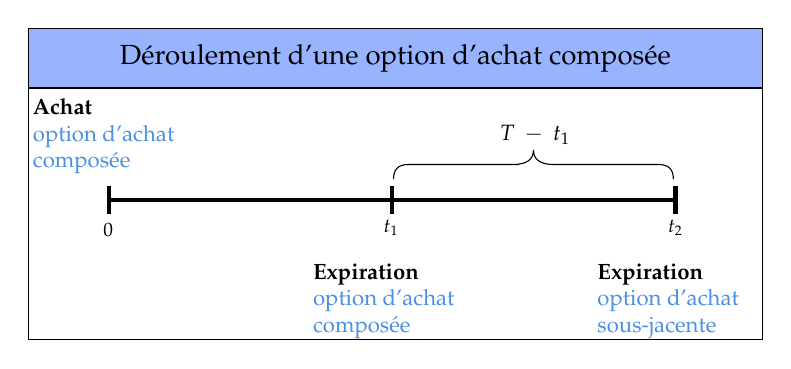
\begin{tikzpicture}[x=0.75pt,y=0.75pt,yscale=-1,xscale=1]
%uncomment if require: \path (0,300); %set diagram left start at 0, and has height of 300

%Shape: Rectangle [id:dp11598225207048363] 
\draw  [fill={rgb, 255:red, 255; green, 255; blue, 255 }  ,fill opacity=1 ] (48,51.33) -- (401.83,51.33) -- (401.83,201.33) -- (48,201.33) -- cycle ;
%Shape: Rectangle [id:dp7987614739910429] 
\draw  [fill={rgb, 255:red, 152; green, 180; blue, 255 }  ,fill opacity=1 ] (48,51.33) -- (401.83,51.33) -- (401.83,80.13) -- (48,80.13) -- cycle ;
%Straight Lines [id:da5349553147510435] 
\draw [line width=1.5]    (86.83,134) -- (359.83,134) ;
\draw [shift={(359.83,134)}, rotate = 180] [color={rgb, 255:red, 0; green, 0; blue, 0 }  ][line width=1.5]    (0,6.71) -- (0,-6.71)   ;
\draw [shift={(223.33,134)}, rotate = 180] [color={rgb, 255:red, 0; green, 0; blue, 0 }  ][line width=1.5]    (0,6.71) -- (0,-6.71)   ;
\draw [shift={(86.83,134)}, rotate = 180] [color={rgb, 255:red, 0; green, 0; blue, 0 }  ][line width=1.5]    (0,6.71) -- (0,-6.71)   ;
%Shape: Brace [id:dp0246391130029624] 
\draw   (358.83,124) .. controls (358.83,119.33) and (356.5,117) .. (351.83,117) -- (301.42,117) .. controls (294.75,117) and (291.42,114.67) .. (291.42,110) .. controls (291.42,114.67) and (288.09,117) .. (281.42,117)(284.42,117) -- (231,117) .. controls (226.33,117) and (224,119.33) .. (224,124) ;

% Text Node
\draw (224.92,65.73) node   [align=left] {Déroulement d'une option d'achat composée};
% Text Node
\draw (49,84.13) node [anchor=north west][inner sep=0.75pt]  [font=\footnotesize] [align=left] {\textbf{Achat}\\\textcolor[rgb]{0.29,0.56,0.89}{option d'achat }\\ \textcolor[rgb]{0.29,0.56,0.89}{composée}};
% Text Node
\draw (184,163.63) node [anchor=north west][inner sep=0.75pt]  [font=\footnotesize] [align=left] {
\textbf{Expiration}\\\textcolor[rgb]{0.29,0.56,0.89}{option d'achat }\\\textcolor[rgb]{0.29,0.56,0.89}{composée}};
% Text Node
\draw (321,163.63) node [anchor=north west][inner sep=0.75pt]  [font=\footnotesize] [align=left] {\textbf{Expiration}\\\textcolor[rgb]{0.29,0.56,0.89}{option d'achat }\\\textcolor[rgb]{0.29,0.56,0.89}{sous-jacente }};
% Text Node
\draw (83,144) node [anchor=north west][inner sep=0.75pt]  [font=\scriptsize] [align=left] {$\displaystyle 0$};
% Text Node
\draw (218,142.5) node [anchor=north west][inner sep=0.75pt]  [font=\scriptsize] [align=left] {$\displaystyle t_{1}$};
% Text Node
\draw (355,142.5) node [anchor=north west][inner sep=0.75pt]  [font=\scriptsize] [align=left] {$\displaystyle t_{2}$};
% Text Node
\draw (274,97) node [anchor=north west][inner sep=0.75pt]  [font=\footnotesize] [align=left] {$\displaystyle T\ -\ t_{1}$};
\end{tikzpicture}
\end{center}
La valeur à l'échéance de l'option \textit{sous-jacente} à $t_{1}$ est dénotée \icbox{$V[S_{t_{1}}, K, \underbrace{T - t_{1}}_{\scriptsize{\shortstack{temps restant\\ avant échéance}}}]$}.\\
La valeur à l'échéance de l'option d'achat \textit{composée} à $t_{1}$ est \icbox{$\max(0, \underbrace{V\left[S_{t_{1}}, K, T - t_{1}\right]}_{\small{\shortstack{$S_{T}$ pour des\\ options classiques}}} - x)$}.
\end{definitionNOHFILLsub}

\begin{definitionNOHFILLsub}[Option de vente composée]
Permet au détenteur de vendre une autre option au prix d'exercice.\\
L'option peut être soit un \og \textit{put on call} \fg{} ou un \og \textit{put on put} \fg{}.

\tcbline
On achète une option de vente composée au temps 0 à un prix d'exercice de $x$ expirant à $t_{1}$.\\ L'option sous-jacente a un prix d'exercice de $K$ et expire à $T$.

\begin{center}
	
\tikzset{every picture/.style={line width=0.75pt}} %set default line width to 0.75pt        

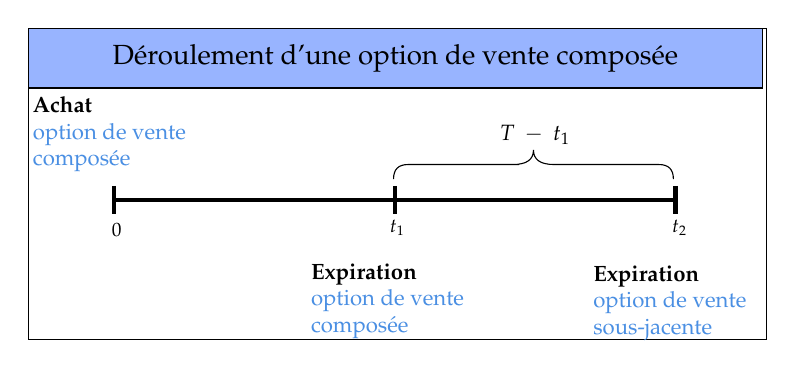
\begin{tikzpicture}[x=0.75pt,y=0.75pt,yscale=-1,xscale=1]
%uncomment if require: \path (0,300); %set diagram left start at 0, and has height of 300

%Shape: Rectangle [id:dp2947812762155695] 
\draw  [fill={rgb, 255:red, 255; green, 255; blue, 255 }  ,fill opacity=1 ] (415,51.33) -- (770.5,51.33) -- (770.5,201.33) -- (415,201.33) -- cycle ;
%Shape: Rectangle [id:dp8558379846670114] 
\draw  [fill={rgb, 255:red, 152; green, 180; blue, 255 }  ,fill opacity=1 ] (415,51.33) -- (768.83,51.33) -- (768.83,80.13) -- (415,80.13) -- cycle ;
%Straight Lines [id:da28206871093985453] 
\draw [line width=1.5]    (456.5,134) -- (726.83,134) ;
\draw [shift={(726.83,134)}, rotate = 180] [color={rgb, 255:red, 0; green, 0; blue, 0 }  ][line width=1.5]    (0,6.71) -- (0,-6.71)   ;
\draw [shift={(591.67,134)}, rotate = 180] [color={rgb, 255:red, 0; green, 0; blue, 0 }  ][line width=1.5]    (0,6.71) -- (0,-6.71)   ;
\draw [shift={(456.5,134)}, rotate = 180] [color={rgb, 255:red, 0; green, 0; blue, 0 }  ][line width=1.5]    (0,6.71) -- (0,-6.71)   ;
%Shape: Brace [id:dp12017435484156325] 
\draw   (725.83,124) .. controls (725.83,119.33) and (723.5,117) .. (718.83,117) -- (668.42,117) .. controls (661.75,117) and (658.42,114.67) .. (658.42,110) .. controls (658.42,114.67) and (655.09,117) .. (648.42,117)(651.42,117) -- (598,117) .. controls (593.33,117) and (591,119.33) .. (591,124) ;

% Text Node
\draw (591.92,65.73) node   [align=left] {Déroulement d'une option de vente composée};
% Text Node
\draw (416,83.13) node [anchor=north west][inner sep=0.75pt]  [font=\footnotesize] [align=left] {\textbf{Achat}\\\textcolor[rgb]{0.29,0.56,0.89}{option de vente }\\\textcolor[rgb]{0.29,0.56,0.89}{composée}};
% Text Node
\draw (550,163.63) node [anchor=north west][inner sep=0.75pt]  [font=\footnotesize] [align=left] {\textbf{Expiration}\\\textcolor[rgb]{0.29,0.56,0.89}{option de vente }\\\textcolor[rgb]{0.29,0.56,0.89}{composée}};
% Text Node
\draw (686,164.63) node [anchor=north west][inner sep=0.75pt]  [font=\footnotesize] [align=left] {\textbf{Expiration}\\\textcolor[rgb]{0.29,0.56,0.89}{option de vente }\\\textcolor[rgb]{0.29,0.56,0.89}{sous-jacente }};
% Text Node
\draw (454,144) node [anchor=north west][inner sep=0.75pt]  [font=\scriptsize] [align=left] {$\displaystyle 0$};
% Text Node
\draw (588,142.5) node [anchor=north west][inner sep=0.75pt]  [font=\scriptsize] [align=left] {$\displaystyle t_{1}$};
% Text Node
\draw (724,142.5) node [anchor=north west][inner sep=0.75pt]  [font=\scriptsize] [align=left] {$\displaystyle t_{2}$};
% Text Node
\draw (641,97) node [anchor=north west][inner sep=0.75pt]  [font=\footnotesize] [align=left] {$\displaystyle T\ -\ t_{1}$};
\end{tikzpicture}
\end{center}
La valeur à l'échéance de l'option de vente \textit{composée} à $t_{1}$ est \icbox{$\max(0, x - V\left[S_{t_{1}}, K, T - t_{1}\right])$}.
\end{definitionNOHFILLsub}

\subsubsection*{Parité}
On généralise l'équation de parité des options vente-achat:
\begin{align*}
	\text{CallonStock}	-	\text{PutonStock}	
	&=	F^{P}(S)	-	K\textrm{e}^{-rT}	\\
	\Rightarrow
	\text{CallonCall}	-	\text{PutonCall}	
	&=	C_{\text{eur}}	-	x\textrm{e}^{-r t_{1}}	\\
	\text{CallonPut}	-	\text{PutonPut}	
	&=	P_{\text{eur}}	-	x\textrm{e}^{-r t_{1}}	\\
\end{align*}


\columnbreak
\subsection{Options avec écart}
\begin{definitionNOHFILL}[Options avec écart]
Contrairement au options classiques qui ont un seul prix pour déterminer le \underline{moment d'exercice} et \underline{la valeur à l'échéance}, les options avec écart ont un prix pour chacune des fonctions créant alors un \textit{écart}.

\begin{distributions}[Notation]
\begin{description}
	\item[$K_{1}$]	Prix \textit{d'exercice} utilisé pour calculer la valeur à l'échéance;
	\item[$K_{2}$]	Prix \textit{déclencheur} utilisé pour décider s'il y a exercice ou pas.
\end{description}
\end{distributions}

\tcbline

\begin{itemize}[leftmargin = *]
	\item	En anglais, \og \textit{gap option} \fg{}.
\end{itemize}
\end{definitionNOHFILL}

\begin{definitionNOHFILLsub}[Option d'achat avec écart]
\begin{align*}
	\shortstack{Valeur à l'échéance}
	&=	\begin{cases}
		0,	&	S_{T}	\leq		K_{2}	\\
		S_{T}	-	K_{1},	&	S_{T}	>		K_{2}	\\
		\end{cases}
\end{align*}

\begin{center}	
\tikzset{every picture/.style={line width=0.75pt}} %set default line width to 0.75pt        

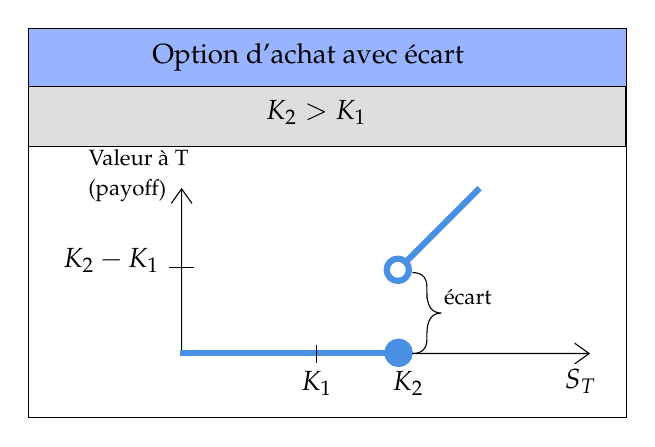
\begin{tikzpicture}[x=0.75pt,y=0.75pt,yscale=-1,xscale=1]
%uncomment if require: \path (0,300); %set diagram left start at 0, and has height of 300

%Shape: Rectangle [id:dp619089624226296] 
\draw  [fill={rgb, 255:red, 255; green, 255; blue, 255 }  ,fill opacity=1 ] (47,11.6) -- (335.17,11.6) -- (335.17,199.33) -- (47,199.33) -- cycle ;
%Shape: Rectangle [id:dp7223985052529034] 
\draw  [fill={rgb, 255:red, 152; green, 180; blue, 255 }  ,fill opacity=1 ] (47,11.6) -- (335.17,11.6) -- (335.17,40.4) -- (47,40.4) -- cycle ;
%Shape: Rectangle [id:dp33113580306042034] 
\draw  [fill={rgb, 255:red, 222; green, 222; blue, 222 }  ,fill opacity=1 ] (47,39.8) -- (334.83,39.8) -- (334.83,68.64) -- (47,68.64) -- cycle ;

%Straight Lines [id:da9695087678158307] 
\draw    (225.42,172.67) -- (225.42,163.67) ;
%Shape: Axis 2D [id:dp6076884557308353] 
\draw  (120.92,168.33) -- (317.25,168.33)(120.92,89) -- (120.92,168.33) -- cycle (310.25,163.33) -- (317.25,168.33) -- (310.25,173.33) (115.92,96) -- (120.92,89) -- (125.92,96)  ;
%Straight Lines [id:da45528019553931376] 
\draw [color={rgb, 255:red, 74; green, 144; blue, 226 }  ,draw opacity=1 ][line width=2.25]    (228.17,124.92) -- (264.42,88.67) ;
\draw [shift={(225.08,128)}, rotate = 315] [color={rgb, 255:red, 74; green, 144; blue, 226 }  ,draw opacity=1 ][line width=2.25]      (0, 0) circle [x radius= 5.36, y radius= 5.36]   ;
%Straight Lines [id:da22765443723573076] 
\draw [color={rgb, 255:red, 74; green, 144; blue, 226 }  ,draw opacity=1 ][line width=2.25]    (120.25,168) -- (225.42,168) ;
\draw [shift={(225.42,168)}, rotate = 0] [color={rgb, 255:red, 74; green, 144; blue, 226 }  ,draw opacity=1 ][fill={rgb, 255:red, 74; green, 144; blue, 226 }  ,fill opacity=1 ][line width=2.25]      (0, 0) circle [x radius= 5.36, y radius= 5.36]   ;
%Straight Lines [id:da7647427977294252] 
\draw    (114.92,127) -- (126.92,127) ;
%Straight Lines [id:da9490135961447259] 
\draw    (186.08,173) -- (186.08,164) ;
%Shape: Brace [id:dp5902887164439852] 
\draw   (232.08,168.33) .. controls (236.75,168.33) and (239.08,166) .. (239.08,161.33) -- (239.08,158.83) .. controls (239.08,152.16) and (241.41,148.83) .. (246.08,148.83) .. controls (241.41,148.83) and (239.08,145.5) .. (239.08,138.83)(239.08,141.83) -- (239.08,136.33) .. controls (239.08,131.66) and (236.75,129.33) .. (232.08,129.33) ;


% Text Node
\draw (313.08,181.67) node   [align=left] {$\displaystyle S_{T}$};
% Text Node
\draw (87.08,123.67) node   [align=left] {$\displaystyle K_{2} -K_{1}$};
% Text Node
\draw (100.08,82.67) node  [font=\small,rotate=-0.4] [align=left] {{\footnotesize Valeur à T }\\{\footnotesize (payoff)}};
% Text Node
\draw (186.08,182.67) node   [align=left] {$\displaystyle K_{1}$};
% Text Node
\draw (230.08,182.67) node   [align=left] {$\displaystyle K_{2}$};
% Text Node
\draw (246.08,136) node [anchor=north west][inner sep=0.75pt]   [align=left] {{\footnotesize écart}};
% Text Node
\draw (160.42,45.22) node [anchor=north west][inner sep=0.75pt]   [align=left] {$\displaystyle K_{2}  >K_{1}$};
% Text Node
\draw (105.58,17.5) node [anchor=north west][inner sep=0.75pt]   [align=left] {Option d'achat avec écart};


\end{tikzpicture}
\end{center}
\end{definitionNOHFILLsub}

\begin{definitionNOHFILLsub}[]
\begin{center}
\tikzset{every picture/.style={line width=0.75pt}} %set default line width to 0.75pt        

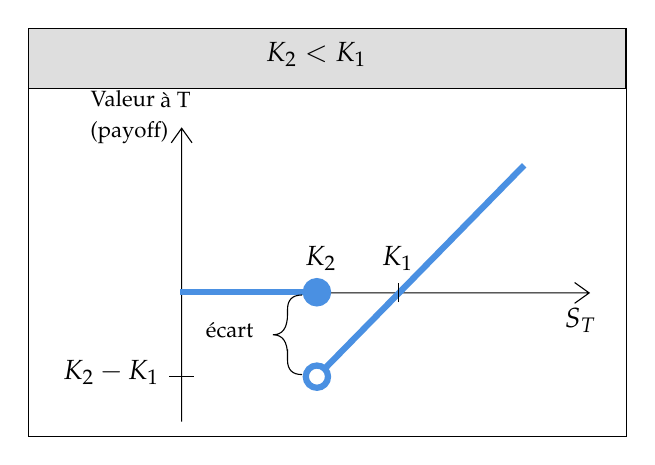
\begin{tikzpicture}[x=0.75pt,y=0.75pt,yscale=-1,xscale=1]
%uncomment if require: \path (0,300); %set diagram left start at 0, and has height of 300

%Shape: Rectangle [id:dp02824851841091225] 
\draw  [fill={rgb, 255:red, 255; green, 255; blue, 255 }  ,fill opacity=1 ] (341,40) -- (629.17,40) -- (629.17,236.33) -- (341,236.33) -- cycle ;
%Shape: Rectangle [id:dp874148547303963] 
\draw  [fill={rgb, 255:red, 222; green, 222; blue, 222 }  ,fill opacity=1 ] (341,39.8) -- (628.83,39.8) -- (628.83,68.64) -- (341,68.64) -- cycle ;
%Straight Lines [id:da24846864702899407] 
\draw    (480.08,172) -- (480.08,163) ;
%Shape: Axis 2D [id:dp21245115433709816] 
\draw  (414.92,167.33) -- (611.25,167.33)(414.92,88) -- (414.92,229.33) (604.25,162.33) -- (611.25,167.33) -- (604.25,172.33) (409.92,95) -- (414.92,88) -- (419.92,95)  ;
%Straight Lines [id:da8962117343156981] 
\draw [color={rgb, 255:red, 74; green, 144; blue, 226 }  ,draw opacity=1 ][line width=2.25]    (483.14,204.55) -- (579.92,105.83) ;
\draw [shift={(480.08,207.67)}, rotate = 314.43] [color={rgb, 255:red, 74; green, 144; blue, 226 }  ,draw opacity=1 ][line width=2.25]      (0, 0) circle [x radius= 5.36, y radius= 5.36]   ;
%Straight Lines [id:da9684164695925033] 
\draw [color={rgb, 255:red, 74; green, 144; blue, 226 }  ,draw opacity=1 ][line width=2.25]    (414.25,167) -- (480.08,167) ;
\draw [shift={(480.08,167)}, rotate = 0] [color={rgb, 255:red, 74; green, 144; blue, 226 }  ,draw opacity=1 ][fill={rgb, 255:red, 74; green, 144; blue, 226 }  ,fill opacity=1 ][line width=2.25]      (0, 0) circle [x radius= 5.36, y radius= 5.36]   ;
%Straight Lines [id:da33212462417226885] 
\draw    (408.92,207.67) -- (420.92,207.67) ;
%Shape: Brace [id:dp4820221483417275] 
\draw   (472.92,168.33) .. controls (468.25,168.33) and (465.92,170.66) .. (465.92,175.33) -- (465.92,177.5) .. controls (465.92,184.17) and (463.59,187.5) .. (458.92,187.5) .. controls (463.59,187.5) and (465.92,190.83) .. (465.92,197.5)(465.92,194.5) -- (465.92,199.67) .. controls (465.92,204.34) and (468.25,206.67) .. (472.92,206.67) ;
%Straight Lines [id:da6332672296521837] 
\draw    (519.42,171.67) -- (519.42,162.67) ;


% Text Node
\draw (607.08,180.67) node   [align=left] {$\displaystyle S_{T}$};
% Text Node
\draw (381.08,205.67) node   [align=left] {$\displaystyle K_{2} -K_{1}$};
% Text Node
\draw (395.08,82.67) node  [font=\small,rotate=-0.4] [align=left] {{\footnotesize Valeur à T }\\{\footnotesize (payoff)}};
% Text Node
\draw (482.08,150.67) node   [align=left] {$\displaystyle K_{2}$};
% Text Node
\draw (519.08,150.67) node   [align=left] {$\displaystyle K_{1}$};
% Text Node
\draw (425.36,180.17) node [anchor=north west][inner sep=0.75pt]   [align=left] {{\footnotesize écart}};
% Text Node
\draw (454.42,45.22) node [anchor=north west][inner sep=0.75pt]   [align=left] {$\displaystyle K_{2}  < K_{1}$};


\end{tikzpicture}
\end{center}
\end{definitionNOHFILLsub}

\begin{definitionNOHFILLsub}[Option de vente avec écart]
\begin{align*}
	\shortstack{Valeur à l'échéance}
	&=	\begin{cases}
		K_{1}	-	S_{T},	&	S_{T}	<		K_{2}	\\
		0,	&	S_{T}	\geq		K_{2}	\\
		\end{cases}
\end{align*}

\begin{center}
\tikzset{every picture/.style={line width=0.75pt}} %set default line width to 0.75pt        

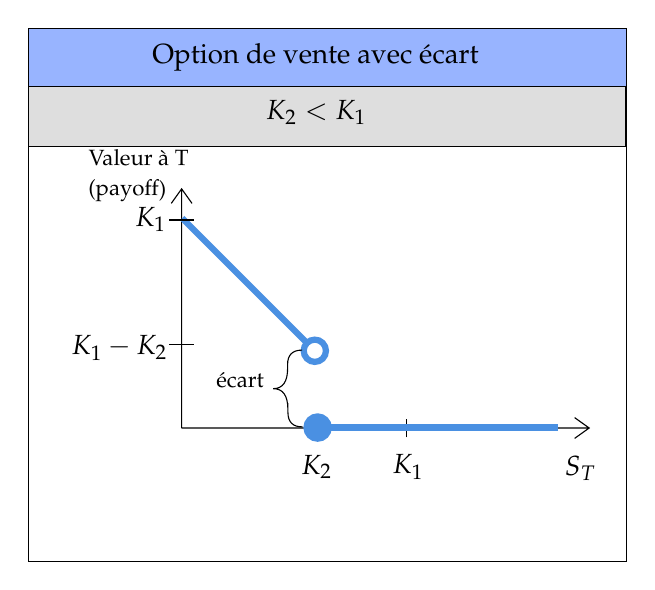
\begin{tikzpicture}[x=0.75pt,y=0.75pt,yscale=-1,xscale=1]
%uncomment if require: \path (0,300); %set diagram left start at 0, and has height of 300

%Straight Lines [id:da6880212768068523] 
\draw    (186.08,210.99) -- (186.08,197.92) ;
%Shape: Rectangle [id:dp533040316964958] 
\draw  [fill={rgb, 255:red, 255; green, 255; blue, 255 }  ,fill opacity=1 ] (47,11.6) -- (335.17,11.6) -- (335.17,268.33) -- (47,268.33) -- cycle ;
%Shape: Rectangle [id:dp3644703127950564] 
\draw  [fill={rgb, 255:red, 152; green, 180; blue, 255 }  ,fill opacity=1 ] (47,11.6) -- (335.17,11.6) -- (335.17,40.4) -- (47,40.4) -- cycle ;
%Shape: Rectangle [id:dp2786749091172711] 
\draw  [fill={rgb, 255:red, 222; green, 222; blue, 222 }  ,fill opacity=1 ] (47,39.8) -- (334.83,39.8) -- (334.83,68.64) -- (47,68.64) -- cycle ;
%Straight Lines [id:da8012392898190628] 
\draw    (229.42,208.67) -- (229.42,199.67) ;
%Shape: Axis 2D [id:dp20357657984540478] 
\draw  (120.92,204.21) -- (317.25,204.21)(120.92,89) -- (120.92,204.21) -- cycle (310.25,199.21) -- (317.25,204.21) -- (310.25,209.21) (115.92,96) -- (120.92,89) -- (125.92,96)  ;
%Straight Lines [id:da27804562364712426] 
\draw [color={rgb, 255:red, 74; green, 144; blue, 226 }  ,draw opacity=1 ][line width=2.25]    (182,163.92) -- (121.17,103.08) ;
\draw [shift={(185.08,167)}, rotate = 225] [color={rgb, 255:red, 74; green, 144; blue, 226 }  ,draw opacity=1 ][line width=2.25]      (0, 0) circle [x radius= 5.36, y radius= 5.36]   ;
%Straight Lines [id:da8757420270721892] 
\draw [color={rgb, 255:red, 74; green, 144; blue, 226 }  ,draw opacity=1 ][line width=2.25]    (302.17,204) -- (186.42,204) ;
\draw [shift={(186.42,204)}, rotate = 180] [color={rgb, 255:red, 74; green, 144; blue, 226 }  ,draw opacity=1 ][fill={rgb, 255:red, 74; green, 144; blue, 226 }  ,fill opacity=1 ][line width=2.25]      (0, 0) circle [x radius= 5.36, y radius= 5.36]   ;
%Straight Lines [id:da5995103411343021] 
\draw    (114.92,104) -- (126.92,104) ;
%Shape: Brace [id:dp27149992922353494] 
\draw   (178.92,166.67) .. controls (174.25,166.7) and (171.93,169.04) .. (171.96,173.71) -- (171.97,175.21) .. controls (172.02,181.88) and (169.71,185.23) .. (165.04,185.26) .. controls (169.71,185.23) and (172.06,188.54) .. (172.11,195.21)(172.09,192.21) -- (172.12,196.71) .. controls (172.15,201.38) and (174.5,203.7) .. (179.17,203.67) ;
%Straight Lines [id:da023586524348984783] 
\draw    (114.92,164) -- (126.92,164) ;

% Text Node
\draw (313.08,223.57) node   [align=left] {$\displaystyle S_{T}$};
% Text Node
\draw (106.08,103.67) node   [align=left] {$\displaystyle K_{1}$};
% Text Node
\draw (100.08,82.67) node  [font=\small,rotate=-0.4] [align=left] {{\footnotesize Valeur à T }\\{\footnotesize (payoff)}};
% Text Node
\draw (186.08,223.03) node   [align=left] {$\displaystyle K_{2}$};
% Text Node
\draw (230.08,223.03) node   [align=left] {$\displaystyle K_{1}$};
% Text Node
\draw (160.42,45.22) node [anchor=north west][inner sep=0.75pt]   [align=left] {$\displaystyle K_{2} < K_{1}$};
% Text Node
\draw (105.58,17.5) node [anchor=north west][inner sep=0.75pt]   [align=left] {Option de vente avec écart};
% Text Node
\draw (136.36,176.17) node [anchor=north west][inner sep=0.75pt]   [align=left] {{\footnotesize écart}};
% Text Node
\draw (91.08,165.67) node   [align=left] {$\displaystyle K_{1} -K_{2}$};


\end{tikzpicture}
\end{center}
\end{definitionNOHFILLsub}

\begin{definitionNOHFILLsub}[]
\begin{center}
\tikzset{every picture/.style={line width=0.75pt}} %set default line width to 0.75pt        

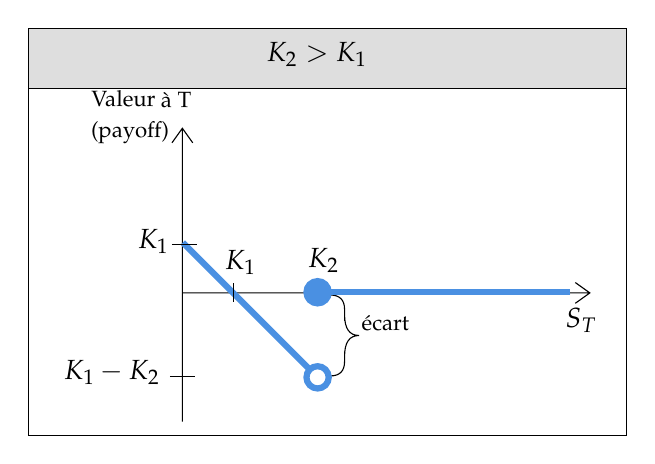
\begin{tikzpicture}[x=0.75pt,y=0.75pt,yscale=-1,xscale=1]
%uncomment if require: \path (0,300); %set diagram left start at 0, and has height of 300

%Shape: Rectangle [id:dp6381171616290457] 
\draw  [fill={rgb, 255:red, 255; green, 255; blue, 255 }  ,fill opacity=1 ] (340.67,39.8) -- (628.83,39.8) -- (628.83,236.13) -- (340.67,236.13) -- cycle ;
%Shape: Rectangle [id:dp7978813517508636] 
\draw  [fill={rgb, 255:red, 222; green, 222; blue, 222 }  ,fill opacity=1 ] (341,39.8) -- (628.83,39.8) -- (628.83,68.64) -- (341,68.64) -- cycle ;
%Straight Lines [id:da9673151320044195] 
\draw    (480.08,172) -- (480.08,163) ;
%Shape: Axis 2D [id:dp9572879435153827] 
\draw  (414.92,167.33) -- (611.25,167.33)(414.92,88) -- (414.92,229.33) (604.25,162.33) -- (611.25,167.33) -- (604.25,172.33) (409.92,95) -- (414.92,88) -- (419.92,95)  ;
%Straight Lines [id:da1159285531737253] 
\draw    (408.92,207.67) -- (420.92,207.67) ;
%Shape: Brace [id:dp46981450240901546] 
\draw   (486.08,207.33) .. controls (490.75,207.33) and (493.08,205) .. (493.08,200.33) -- (493.08,197.83) .. controls (493.08,191.16) and (495.41,187.83) .. (500.08,187.83) .. controls (495.41,187.83) and (493.08,184.5) .. (493.08,177.83)(493.08,180.83) -- (493.08,175.33) .. controls (493.08,170.66) and (490.75,168.33) .. (486.08,168.33) ;
%Straight Lines [id:da44587483028780883] 
\draw [color={rgb, 255:red, 74; green, 144; blue, 226 }  ,draw opacity=1 ][line width=2.25]    (477,204.92) -- (415.17,143.08) ;
\draw [shift={(480.08,208)}, rotate = 225] [color={rgb, 255:red, 74; green, 144; blue, 226 }  ,draw opacity=1 ][line width=2.25]      (0, 0) circle [x radius= 5.36, y radius= 5.36]   ;
%Straight Lines [id:da40306089301904247] 
\draw    (409.92,144) -- (421.92,144) ;
%Straight Lines [id:da8412289279627245] 
\draw [color={rgb, 255:red, 74; green, 144; blue, 226 }  ,draw opacity=1 ][line width=2.25]    (601.83,167) -- (480.08,167) ;
\draw [shift={(480.08,167)}, rotate = 180] [color={rgb, 255:red, 74; green, 144; blue, 226 }  ,draw opacity=1 ][fill={rgb, 255:red, 74; green, 144; blue, 226 }  ,fill opacity=1 ][line width=2.25]      (0, 0) circle [x radius= 5.36, y radius= 5.36]   ;
%Straight Lines [id:da13309232440240026] 
\draw    (439.42,171.67) -- (439.42,162.67) ;

% Text Node
\draw (607.08,180.67) node   [align=left] {$\displaystyle S_{T}$};
% Text Node
\draw (381.08,205.67) node   [align=left] {$\displaystyle K_{1} -K_{2}$};
% Text Node
\draw (395.08,82.67) node  [font=\small,rotate=-0.4] [align=left] {{\footnotesize Valeur à T }\\{\footnotesize (payoff)}};
% Text Node
\draw (443.08,152.67) node   [align=left] {$\displaystyle K_{1}$};
% Text Node
\draw (483.08,151.67) node   [align=left] {$\displaystyle K_{2}$};
% Text Node
\draw (454.42,45.22) node [anchor=north west][inner sep=0.75pt]   [align=left] {$\displaystyle K_{2}  >K_{1}$};
% Text Node
\draw (500.08,177) node [anchor=north west][inner sep=0.75pt]   [align=left] {{\footnotesize écart}};
% Text Node
\draw (401.08,142.67) node   [align=left] {$\displaystyle K_{1}$};


\end{tikzpicture}
\end{center}
\end{definitionNOHFILLsub}

\begin{itemize}[leftmargin = *]
	\item	Il est possible d'avoir une valeur à l'échéance \textit{négative} si le prix déclencheur $K_{2}$ est inférieur au prix  d'exercice $K_{1}$ pour une option d'achat (ou si $K_{1} < K_{2}$ pour une option de vente);
	\item	Cependant, même si la valeur à l'échéance est négative, l'exercice est obligatoire lorsque le prix déclencheur est atteint;
	\item	Cela dit, il est en revanche possible d'avoir une \textbf{prime négative}.
\end{itemize}

\subsubsection*{Formule de Black-Scholes}
On substitue le $K$ dans l'équation principale pour le prix d'exercice $K_{1}$ et le $K$ dans l'équation de $d_{1}$ pour le prix déclencheur $K_{2}$.
\begin{align*}
	\text{GapCall}
	&=	S_{0} \textrm{e}^{- \delta T} N(d_{1}) - K_{1}\textrm{e}^{-rT} N(d_{2})	\\
	\text{GapPut}
	&=	K_{1}\textrm{e}^{-rT} N(-d_{2}) - S_{0}\textrm{e}^{-\delta T}N(-d_{1})	
\end{align*}
où $d_{1}	=	\frac{\ln\left(\frac{S_{0}}{K_{2}}\right) + \left( r - \delta + \frac{1}{2} \sigma^{2} \right)T}{\sigma \sqrt{T}}$ et $d_{2}	=	d_{1} - \sigma \sqrt{T}$.\\

Pour se rappeler quel $K$ remplacer:
\begin{itemize}[leftmargin = *]
	\item	Le prix d'exercice $K_{1}$ détermine le montant de la valeur à l'échéance et est donc associé avec $K\textrm{e}^{-rT}$ dans l'équation principale;
	\item	Le prix déclencheur $K_{2}$ détermine si l'exercice a lieu et est donc associé avec le calcul d'une probabilité $N(d_{2})$.
\end{itemize}

\subsubsection*{Relation avec les options classiques}
\begin{align*}
	\text{GapCall}	\pm	K_{2}\textrm{e}^{-rT} N(d_{2})
	&=	C_{\text{eur}}(K_{2})	+	(K_{2}	-	K_{1})\textrm{e}^{-rT} N(d_{2})	\\
	\text{GapPut}	\pm	K_{2}\textrm{e}^{-rT} N(-d_{2})
	&=	P_{\text{eur}}(K_{2})	+	(K_{1}	-	K_{2})\textrm{e}^{-rT} N(-d_{2})
\end{align*}

\subsubsection*{Parité}
\begin{align*}
	\text{GapCall}	-	\text{GapPut}
	&=	S_{0}\textrm{e}^{-\delta T}	-	K_{1}\textrm{e}^{-rT}
\end{align*}

\columnbreak
\subsection{Options d'échange}
\begin{definitionNOHFILL}[Options d'échange]
Permet au détenteur d'échanger un actif pour un autre.

\tcbline

\begin{itemize}[leftmargin = *]
	\item	En anglais, \og \textit{exchange option} \fg{}.
\end{itemize}
\end{definitionNOHFILL}

\subsubsection*{Formule de Black-Scholes}
Formule en format simple et selon la notation de Claire où l'on achète $k$ du titre $Q$ par unité du titre $S$
\begin{align*}
	C(A, B)
	&=	F^{P}(A)N(d_{1})	-	F^{P}(A)N(d_{2})	\\
	&=	S_{0} \textrm{e}^{-\delta_{S}T}N(d_{1})	-	kQ_{0} \textrm{e}^{-\delta_{Q}T}N(d_{2})	\\
	P(A, B)
	&=	F^{P}(B)N(-d_{2})	-	F^{P}(A)N(-d_{1})	\\
	&=	kQ_{0} \textrm{e}^{-\delta_{Q}T}N(d_{1})	-	S_{0} \textrm{e}^{-\delta_{S}T}N(d_{2})	\\	
\end{align*}

où $d_{1}	=	\frac{\ln\left(\frac{F^{P}(A)}{F^{P}(B)}\right) + \frac{1}{2} \sigma^{2} T}{\sigma \sqrt{T}}$, $d_{2}	=	d_{1} - \sigma \sqrt{T}$ et \icbox{$\sigma	=	\sqrt{\sigma^{2}_{A} + \sigma^{2}_{B}	-	2\rho\sigma_{A}\sigma_{B}}$}.
\begin{itemize}
	\item	On note que \textbf{l'on soustrait} la corrélation puisque le portefeuille est $A	-	B$.
\end{itemize}

\pagebreak
\setcounter{section}{17}
\section{La loi lognormale}
\label{sec:lognorm}
\begin{distributions}[Notation]
\begin{description}
	\item[$N(d)$]	Représente $Pr(Z \leq d)$.
\end{description}
\end{distributions}


\subsection{La distribution normale}
\begin{itemize}[leftmargin = *]
	\item	Si $X \sim \mathcal{N}(\mu, \sigma^{2})$ alors \lfbox[formula]{$Z = \frac{X - \mu}{\sigma} \sim \mathcal{N}(0, 1)$};
	\item	La loi normale est symétrique donc \lfbox[formula]{$N(-d) = 1 - N(d)$}, \lfbox[conditions]{$\forall d \in \mathbb{R}$} et \lfbox[formula]{$\Pr(-d \leq Z \leq d)	=	2N(d)	-	1$}, \lfbox[conditions]{$\forall d \in \mathbb{R}_{+}$};
	\item	\lfbox[formula]{$aX_{1} + bX_{2}	\sim	\mathcal{N}(a\mu_{1} + b\mu_{2}, a^{2}\sigma^{2}_{1} + b^{2}\sigma^{2}_{2} + 2ab\rho\sigma_{1}\sigma_{2})$};
	\item	La FGM est $M_{X}(t)	=	\textrm{e}^{\mu t + \frac{\sigma^{2} t^{2}}{2}}$.
\end{itemize}


\subsection{La distribution lognormale}
Lorsque $Y = \textrm{e}^{X}$ alors $Y \sim LN(\mu,\sigma^{2})$.

\begin{itemize}
	\item	Les deux premiers moments sont obtenus de la FGM de la distribution normale et ne sont \textbf{\textit{pas}} les paramètres:
		\begin{align*}
		\text{E}[Y]
		&=	\textrm{e}^{\mu + \frac{1}{2}\sigma^{2}}	&
		\text{Var}(Y)
		&=	\left(\text{E}[Y]\right)^{2} \left(\textrm{e}^{\sigma^{2}} - 1\right)	
		\end{align*}
	\item	\lfbox[formula]{$F_{Y}(y)	=	N\left(\frac{\ln(y) - \mu}{\sigma}\right)$}, \lfbox[conditions]{$\forall y \in \mathbb{R}_{+}$}.
\end{itemize}

La distribution lognormale a 2 propriétés intéressantes:
\begin{enumerate}[leftmargin = *]
	\item	Elle est asymétrique à droite et donc \textbf{\textit{non-négative}} puisque $\textrm{e}^{X} \ge 0$:
		\begin{align*}
		\text{E}[Y]
		=	\text{E}[\textrm{e}^{X}]
		\geq
		\textrm{e}^{\text{E}[X]}
		=	\textrm{e}^{\text{E}[\ln(Y)]}
		\end{align*}
		\begin{itemize}[leftmargin = *]
		\item	Alors supposer que le prix d'une action suit une distribution lognormale suppose qu'il ne peut pas être négatif (une hypothèse réaliste).
		\end{itemize}
	\item	Le \textit{\textbf{produit}} \underline{(et non la somme)} de deux variables aléatoires lognormales est une variable aléatoire.
		\begin{itemize}[leftmargin = *]
		\item	$X_{1} + X_{2} \sim \mathcal{N}$
		\item	$\textrm{e}^{X_{1}} 	\times \textrm{e}^{X_{2}} \sim LN$
		\end{itemize}
\end{enumerate}


\columnbreak
\subsection*{Un modèle lognormale des prix de l'action}
\subsubsection*{Introduction}
\begin{distributions}[Notation]
\begin{description}
	\item[$R(0, t)$]	Rendement composé continûment entre $0$ et $t$ sur un titre donné;
		\begin{itemize}
		\item	Par définition, \lfbox[formula]{$R(0, T)	=	\ln\left(\frac{S_{t}}{S_{0}}\right)$};
		\item	On suppose que $R_{0, t}$ suit une loi normale et donc il s'ensuit que $S_{t}$ suit une loi lognormale.
		\end{itemize}
\end{description}
\end{distributions}

\begin{itemize}
	\item	Avec les propriétés des exposants, on trouve que $S_{t_{2}}	=	S_{t_{1}}\textrm{e}^{R(t_{1}, t_{2})}	=	S_{t_{0}}\textrm{e}^{R(t_{0}, t_{1}) + R(t_{1}, t_{2})}$;
	\item	Avec la propriété de la loi normale, on trouve que \lfbox[formula]{$R(0, T)	=	\sumz{n}{i	=	1}R\left((i	-	1)h, ih\right)$} où les rendements sont (i.i.d.) pour $i	=	1, 2, \dots, n$;
	\item	Avec $R\left((i	-	1)h, ih\right) \sim \mathcal{N}(\mu_{h}, \sigma^{2}_{h})$ pour $i	=	1, 2, \dots, n$, $R(0, T) \sim \mathcal{N}(n\mu_{h}, n\sigma^{2}_{h})$.	\\
			C'est-à-dire que la moyenne et la variance des rendements sont \textit{proportionnels au temps};	
	\item	Sous base annuelle, $\mu =	\frac{\mu_{h}}{h}$ et $\sigma =	\frac{\sigma_{h}}{\sqrt{h}}$ donc \lfbox[formula]{$R(0, T) \sim \mathcal{N}(\mu_{h}T, \sigma^{2}_{h}T)$}.
\end{itemize}

De façon générale, on suppose que le \lfbox[tight, background-color = palechestnut!60!white, border-color = white]{temps $t$ est mesuré en années}, que \lfbox[tight, background-color = palechestnut!60!white, border-color = white]{la moyenne $\alpha$ et la volatilité (variance) $\sigma^{2}$ sont sous base annuelle} puis que le \lfbox[tight, background-color = palechestnut!60!white, border-color = white]{taux de dividendes sur l'action $\delta$ est sous base annuelle} aussi.

\subsubsection*{Modèle}
On cherche $\text{E}[S_{t}]	=	S_{0}\textrm{e}^{(\alpha - \delta)t}$


\begin{definitionNOHFILL}[Distribution]
On pose que le gain en capital composé continûment de $0$ à $t$ $\ln\left(\frac{S_{t}}{S_{0}}\right)$ est normalement distribué: \\
\begin{align*}
	\ln\left(\frac{S_{t}}{S_{0}}\right) 
	&\sim	\mathcal{N}\left(\Big(\alpha - \delta - \frac{1}{2}\sigma^{2}\Big)t, \sigma^{2}t\right)	\\
\end{align*}

On écrit donc:
\begin{align*}
	S_{t} 
	&=	S_{0}\textrm{e}^{(\alpha - \delta - \frac{1}{2}\sigma^{2})t + \sigma\sqrt{t}Z}
\end{align*}
\end{definitionNOHFILL}

\begin{definitionNOHFILLsub}[Moyenne variance et covariance]
Avec cette distribution, on obtient:
\begin{align*}
	\text{E}[S_{t}]
	&=	S_{0}\textrm{e}^{(\alpha - \delta)t}		\\
	\Rightarrow
	\ln\text{E}\left[\frac{S_{t}}{S_{0}}\right]
	&=	(\alpha - \delta)t
\end{align*}
\begin{itemize}
	\item	Il est désirable que l'espérance ne dépend pas de la volatilité $\sigma$;
	\item	En fait, on soustrait $\frac{1}{2}\sigma^{2}$ dans le paramètre $\mu$ afin qu'il s'annule dans le calcul de l'espérance de la loi lognormale;
	\item	La quantité $\alpha	-	\delta$ est le \lfbox[tight, background-color = palechestnut!60!white, border-color = white]{taux d'appréciation de l'action composé continûment}.
\end{itemize}
\begin{align*}
	\text{Var}(S_{t})
	&=	\left(\text{E}[S_{t}]\right)^{2} \left(\textrm{e}^{\sigma^{2}t} - 1\right)	\\
	Cov(S_{t}, S_{t})
	&=	\text{E}\left[\frac{S_{t}}{S_{t}}\right] \cdot \text{Var}(S_{t})	
	=	\textrm{e}^{(\alpha - \delta)(T - t)} \text{Var}(S_{t})
\end{align*}
\end{definitionNOHFILLsub}

\begin{distributions}[Trouver le $p$-ème percentile de $S_{t}$]
\begin{enumerate}[leftmargin = *]
	\item	Trouver le percentile correspondant $z_{\alpha}$ de la loi normale standard $Z$.
	\item	Insérer le percentile correspondant de $Z$ dans l'équation pour $S_{t}$.
\end{enumerate}
\end{distributions}

\textbf{La médiane}:
\begin{itemize}
	\item	La médiane \lfbox[formula]{$\text{E}[S_{t}]\textrm{e}^{-\frac{1}{2}\sigma^{2}t}$} est inférieure à la moyenne;
	\item	Alors, une action distribuée selon la loi lognormale aura des rendements inférieurs à la moyenne plus que la moité du temps;
	\item	Il s'ensuit qu'augmenter $\sigma$ ne va pas impacter la moyenne mais va faire \textit{baisser la médiane}.
\end{itemize}

\textbf{Déplacement d'un écart type}:\\
En posant $Z_{i}	=	\pm 1$, on trouve qu'un déplacement d'un écart type de $S_{(i - 1)h}$ est $S_{ih}	=	S_{(i - 1)h}\textrm{e}^{(\alpha	-	\delta	-	\frac{1}{2}\sigma^{2})h \pm \sigma \sqrt{h}}$


\columnbreak
\subsection*{Calculs de probabilités lognormales}
On pose:
\begin{align*}
	\hat{d}_{1}
	&=	\left(
			\frac{\ln\frac{S_{0}}{K} + (\alpha - \delta {\color{blue}+} \frac{1}{2}\sigma^{2})t}
	 			 {\sigma\sqrt{t}}
		\right)	&
	\hat{d}_{2}
	&=	\left(
			\frac{\ln\frac{S_{0}}{K} + (\alpha - \delta {\color{red}-} \frac{1}{2}\sigma^{2})t}
	 			 {\sigma\sqrt{t}}
		\right)
\end{align*}

\begin{distributions}[Trouver une probabilité pour $S_{t}$]
\begin{align*}
	\Pr(S_{t}	\leq		K) 
	&=	N(-\hat{d_{2}})	&
	\Pr(S_{t}	>		K) 
	&=	N(\hat{d_{2}})	\\
	\text{Pr}^{*}(S_{t}	\leq		K) 
	&=	N(-d_{2})	&
	\text{Pr}^{*}(S_{t}	>		K) 
	&=	N(d_{2})	
\end{align*}
\end{distributions}

%%%	----------------------------------------------------------
%%%	Je juge un peu trop pour le cadre de la cheathseet (AJVR)
%\begin{algo}{Comment trouver une probabilité avec $S_{t}$}
%\begin{enumerate}[leftmargin = *]
%	\item	Isoler la distribution normale $\ln\left(\frac{S_{t}}{S_{0}}\right)$;
%		\begin{align*}
%		\Pr(S_{t} < K)
%		&=	\Pr\left( \ln\frac{S_{t}}{S_{0}} < \ln\frac{S_{t}}{S_{0}} \right)
%		\end{align*}
%	\item	Centrer et réduire pour obtenir la distribution normale standard $Z$.
%		\begin{align*}
%		\Pr(S_{t} < K)
%		&=	\Pr\left( \frac{\ln\frac{S_{t}}{S_{0}} - m}{v} < \frac{\ln\frac{K}{S_{0}} - (\alpha - \delta - \frac{1}{2}\sigma^{2})t}{\sigma\sqrt{t}}\right)	\\
%		&=	\Pr\left( Z < - {\color{teal}\left(
%				\frac{\ln\frac{S_{0}}{K} + (\alpha - \delta - \frac{1}{2}\sigma^{2})t}{\sigma\sqrt{t}}\right)}
%				\right)	\\
%		&=	\Pr\left( Z < - {\color{teal}\hat{d_{2}}}\right)	\\
%		&=	N(-\hat{d_{2}})
%		\end{align*}
%\end{enumerate}
%\end{algo}
%%%	----------------------------------------------------------

\begin{distributions}[Trouver un intervalle de prévision de $S_{t}$ de niveau $1 - \alpha$]
\begin{enumerate}[leftmargin = *]
	\item	Trouver le percentile correspondant de la loi normale standard $Z$ \lfbox[formula]{$\textcolor{burntorange}{z_{\alpha/2}}	=	N^{-1}\left(1		-	\frac{\alpha}{2}\right)$}.
	\item	Insérer le percentile correspondant dans l'équation pour \lfbox[formula]{$S_{t}	\in	S_{0}\textrm{e}^{(\alpha - \delta - \frac{1}{2}\sigma^{2})t \textcolor{burntorange}{\pm z_{\alpha/2}}\sigma\sqrt{t}}$}.
\end{enumerate}
\end{distributions}

\begin{conceptgen_enhanced}[Espérance conditionnelle du prix de l'action]
%Nous avons l'espérance du prix lorsque l'action est hors-du-cours et dans le cours
\begin{align*}
	\text{E}[S_{t} | S_{t} \leq K]
	&=	\frac{\text{E}\left[S_{t} \times \bm{1}_{\{ S_{t} \leq K \}}\right]}{\Pr(S_{t} \leq K)}
	=	S_{0}\textrm{e}^{(\alpha - \delta)t} \frac{N(-\hat{d}_{1})}{N(-\hat{d}_{2})}	\\
	\text{E}[S_{t} | S_{t} > K]
	&=	\frac{\text{E}\left[S_{t} \times \bm{1}_{\{ S_{t} > K \}}\right]}{\Pr(S_{t} > K)}
	=	S_{0}\textrm{e}^{(\alpha - \delta)t} \frac{N(\hat{d}_{1})}{N(\hat{d}_{2})}		\\
\end{align*}
\begin{align*}
	\text{E}^{*}[S_{t} | S_{t} \leq K]
	&=	S_{0}\textrm{e}^{(r - \delta)t} \frac{N(-d_{1})}{N(-d_{2})}	&
	\text{E}^{*}[S_{t} | S_{t} > K]
	&=	S_{0}\textrm{e}^{(r - \delta)t} \frac{N(d_{1})}{N(d_{2})}	
\end{align*}
\end{conceptgen_enhanced}

\begin{definitionNOHFILL}[Formule de Black-Scholes pour le prix d'options européennes]
Avec ces espérances, on trouve maintenant:
\begin{align*}
	C(K)
	&=	\textrm{e}^{-r T}\text{E}^{*}[\text{valeur à l'échéance de l'option d'achat}]	\\
	&=	S_{0} \textrm{e}^{-\delta T}N(d_{1}) - K\textrm{e}^{-r T} N(d_{2})	\\
	P(K)
	&=	\textrm{e}^{-r T}\text{E}^{*}[\text{valeur à l'échéance de l'option de vente}]	\\
	&=	K\textrm{e}^{-r T} N(-d_{2}) - S_{0} \textrm{e}^{-\delta T}N(-d_{1})	
\end{align*}
\end{definitionNOHFILL}

\begin{conceptgen}{Énoncés équivalents}
\begin{itemize}[leftmargin = *]
	\item	Le modèle de Black-Scholes s'applique.
	\item	Le prix de l'action suit un modèle lognormale.
	\item	$\ln\left(\frac{S_{t}}{S_{0}}\right) \sim \mathcal{N}\left(m = \Big(\alpha - \delta - \frac{1}{2}\sigma^{2}\Big)t, v^{2} = \sigma^{2}t\right)$.
	\item	$S_{t} =	S_{0}\textrm{e}^{(\alpha - \delta - \frac{1}{2}\sigma^{2})t + \sigma\sqrt{t}Z}$.
\end{itemize}
\end{conceptgen}

\columnbreak
\subsection*{Estimation des paramètres (le rendement et la volatilité) de la loi lognormale}
Soit $n + 1$ prix observés $S_{0}, S_{1}, \dots, S_{n}$ à un intervalle régulier de longueur $h$.
\begin{itemize}
	\item	Typiquement, \lfbox[formula]{$h	=	1$}
\end{itemize}

\begin{definitionNOHFILL}[Estimation des paramètres de la distribution lognormale]
\begin{enumerate}
	\item	Calculer le rendement composé continûment, non annualisé, pour chacune des $i$ périodes:
		\begin{align*}
		r_{i}
		&=	\ln\left(\frac{S_{ih}}{S_{(i - 1)}}\right), \, \forall i = 1, 2, \dots, n
		\end{align*}
	\item	Calculer la moyenne de l'échantillon des rendements.
		\begin{align*}
		\bar{r}
		&=	\frac{\overset{n}{\underset{i = 1}{\sum}} r_{i}}{n}	
		\underset{\tiny{\shortstack{propriété\\ des log.}}}{=}	\frac{\ln\left(\frac{S_{n}}{S_{0}}\right)}{n}
		\end{align*}
	\item	Estimer l'écart-type des rendements.
		\begin{align*}
		s_{r}
		&=	\sqrt{\frac{\overset{n}{\underset{i = 1}{\sum}} (r_{i} - \bar{r})^{2}}{n - 1}}
		\end{align*}
	\item	Mettre l'estimation de la volatilité sous base annuelle.
		\begin{align*}
		\hat{\sigma}
		&=	\frac{s_{r}}{\sqrt{h}}
		\end{align*}
	\item	Mettre l'estimation du rendement espéré sous base annuelle.
		\begin{align*}
		\text{E}\left[\ln\left(\frac{S_{t + h}}{S_{t}}\right)\right]
		&=
		\left(\hat{\alpha} - \delta - \frac{1}{2} \hat{\sigma}^{2}\right)h	
		=	\bar{r}	\\
		\therefore \hat{\alpha}	&=	\frac{\bar{r}}{h} + \delta + \frac{1}{2} \hat{\sigma}^{2}
		\end{align*}
\end{enumerate}
\end{definitionNOHFILL}

\pagebreak
\section{Évaluation par la méthode de Monte Carlo}
Lorsque la valeur à l'échéance dépend de la trajectoire du prix, le modèle binomiale devient trop compliqué et nous utilisons plutôt la méthode de Monte Carlo; on simule des prix pour estimer le prix (alias la valeur espérée actualisée) de l'option.

La méthode de Monte Carlo utilise la distribution neutre au risque et le taux sans risque.

\subsection{Calcul du prix de l'option comme une valeur espérée actualisée}
\begin{distributions}[Notation]
\begin{description}
	\item[$\text{E}_{0}^{*}$]	Espérance calculée à $t	=	0$ en utilisant la distribution neutre au risque;
	\item[$V(S_{T}, T)$]	Valeur à l'échéance d'une option dont la valeur du sous-jacent à $T$ est $S_{T}$;
	\item[$V(S_{0}, 0)$]	Prix de l'option;
		\begin{itemize}[leftmargin = *]
		\item	On calcul le prix de l'option avec une évaluation neutre au risque et donc on pose que le rendement est égale au taux sans risque.
		\end{itemize}
		\begin{align*}
		V(S_{0}, 0)	
		&=	\textrm{e}^{-rT}\text{E}_{0}^{*}[V(S_{T}, T)]
		\end{align*}
\end{description}
\end{distributions}

\subsubsection*{Évaluation avec des probabilités neutres au risque}
Pour évaluer une option avec la méthode binomiale, on calcule la valeur à l'échéance à chacun des nœuds sur $n$ périodes puis on pondère par la probabilité d'y arriver et actualise:
\begin{align*}
	C
	&=	\textrm{e}^{-rT} \sum_{i	=	0}^{n} \binom{n}{i} (p^{*})^{n	-	i}(1	-	p^{*})^{i} \max(0;	S_{0}u^{n	-	i}d^{i}	-	K)	\\
	P
	&=	\textrm{e}^{-rT} \sum_{i	=	0}^{n} \binom{n}{i} (p^{*})^{n	-	i}(1	-	p^{*})^{i} \max(0;	K	-	S_{0}u^{n	-	i}d^{i})	
\end{align*}

\subsubsection*{Évaluation des vraies probabilités}
On remplace $p^{*}$ par $p$ cependant, au lieu d'appliquer $\textrm{e}^{-rT}$ à tous, il faut utiliser un différent rendement pour chaque trajectoire.


\columnbreak
\subsection{Génération de nombres aléatoires}
On simule des chiffres $u$ provenant d'une distribution uniforme $U(a, b)$. Lorsque la distribution est $U(0, 1)$, on peut interpréter les chiffres $u$ comme des quantiles et obtenir des valeurs $F^{-1}(u)$ pour une distribution (Méthode de l'inverse).

\subsection{Simulation de prix lognormaux}
On rappel que \lfbox[rappel]{$S_{T}	=	S_{0}\textrm{exp}\left\{ (\alpha - \delta - \frac{1}{2}\sigma^{2})T + \sigma\sqrt{T} Z \right\}$.}
Pour simuler des prix lognormaux $S_{T}$ on insère des valeurs aléatoire de $Z \sim \mathcal{N}(0, 1)$ dans la formule.

\subsubsection*{Simulation d'une séquence de prix d'action}
Si la valeur à l'échéance d'une option dépend de celle du sous-jacent à différents moments dans le temps, il faut simuler des trajectoires pour trouver le prix.\\

Soit une option venant à échéance à $T$ dont la valeur dépend de celle du sous-jacent à $n$ moments (également espacés entre $0$ et $T$). 
\begin{align*}
	S_{h}	
	&=	S_{0}\textrm{exp}\left\{ (\alpha - \delta - \frac{1}{2}\sigma^{2})T + \sigma\sqrt{T} Z_{1} \right\}	\\
	S_{jh}	
	&=	S_{(j - 1)h}\textrm{exp}\left\{ (\alpha - \delta - \frac{1}{2}\sigma^{2})T + \sigma\sqrt{T} Z_{j} \right\},	\quad	\lfbox[conditions]{$j	=	2, 3, \dots, n$}
\end{align*}

Donc, \lfbox[formula]{$S_{nh}	=	S_{T}	=	S_{0}\textrm{exp}\left\{ (\alpha - \delta - \frac{1}{2}\sigma^{2})T + \sqrt{T}\sigma\frac{1}{\sqrt{n}} \sumz{n}{j	=	1}Z_{j} \right\}$} où \lfbox[conditions]{$\frac{1}{\sqrt{n}} \sumz{n}{j	=	1}Z_{j}	\sim	\mathcal{N}(0, 1)$.}


\columnbreak
\subsection{Évaluation par la méthode de Monte Carlo}
\begin{distributions}[Notation]
\begin{description}
	\item[$S_{T}(i)$]	Prix du sous-jacent à $T$ généré aléatoirement avec la distribution neutre au risque;
		\begin{itemize}
		\item	On pose que le prix du sous-jacent suit une distribution neutre au risque en posant 
 \lfbox[conditions]{$\alpha	=	r$}.
		\end{itemize}
	\item[$V(S_{T}(i), T)$]	Valeur à l'échéance de l'option selon la simulation $i$, \lfbox[formula]{$V(S_{T}(i), T)	=	\max(0; S_{T}(i)	-	K)$}.
\end{description}
\end{distributions}

On trouve que selon la méthode de Monte Carlo, \lfbox[formula]{$V(S_{0}, 0)	=	\textrm{e}^{-rT}  \frac{1}{N} \sumz{N}{i	=	1} V(S_{T}(i), T)$.}

\subsubsection*{Évaluation par la méthode de Monte Carlo d'une option d'achat européenne}
L'estimation du prix de l'option est donc:
\begin{align*}
	\overline{C}
	&=	\textrm{e}^{-rT} \frac{1}{N} \sumz{N}{i	=	1} \max(0; S_{T}(i)	-	K)
\end{align*}

\begin{distributions}[Notation]
\begin{description}
	\item[$\sigma_{C}$]	Écart-type de $C$ basé sur une seule simulation;
		\begin{itemize}
		\item	On peut l'estimer par \lfbox[formula]{$s_{c}	=	\sqrt{\frac{1}{N	-	1}\sumz{N}{i	=	1} \left\{ C(S_{T}(i))	-	\overline{C} \right\}^{2}}$}.
		\end{itemize}
	\item[$\sigma_{\overline{C}}$]	Écart-type de $C$ basé sur $N$ simulations, $\sigma_{\overline{C}}	=	\frac{1}{\sqrt{N}}\sigma_{C}$.
\end{description}
\end{distributions}

\subsubsection*{Option sur moyenne (\og \textit{asian} \fg{}) arithmétique}
On estime le prix tel que illustré à la section 19.3 puis on trouve que l'estimé du prix de l'option est \lfbox[formula]{$\overline{AC}	=	\textrm{e}^{-rT} \times \frac{1}{N} \sumz{N}{i	=	1} \max\left(0; \frac{1}{n} \sumz{n}{j	=	1}S_{jh}(i)	-	K\right)$}.


\columnbreak
\subsection{Évaluation par la méthode efficace de Monte Carlo}
La méthode décrite jusqu'ici est la méthode simple (alias, naïve) de Monte Carlo. Il existe des méthodes pour améliorer la précision, et donc réduire la variance de l'estimé.

\subsubsection*{Variable de contrôle}
L'idée de la variable de contrôle est d'estimer l'erreur à chaque itération avec le prix d'une option reliée dont le prix peut être calculé par la formule. On peut ensuite appliquer cette erreur pour améliorer la précision du prix Monte Carlo.

\begin{distributions}[Notation]
\begin{description}
	\item[$A(i)$ et $G(i)$]	Prix de l'option avec moyenne arithmétique et géométrique calculé avec la $i^{\text{e}}$ trajectoire simulée;
	\item[$\overline{A}$ et $\overline{G}$]	Estimé du prix de l'option;
	\item[$A$ et $G$]	Vrai prix de l'option avec moyenne arithmétique et géométrique selon la formule connue;	
		\begin{itemize}
		\item	$A$ est inconnu mais $G$ l'est.
		\end{itemize}
	\item[$A^{*}$]	Estimé ajusté du prix de l'option utilisant la moyenne arithmétique.
\end{description}
\end{distributions}

Pour approximer le prix $A^{*}$ :
\begin{enumerate}
	\item	On pose que $A$ et $G$ sont corrélés et les relient par le coefficient $\beta$.
		\begin{itemize}
		\item	Le coefficient $\beta$ est la pente d'une régression linéaire;
		\item	On trouve donc que $\hat{\beta}	=	\frac{\text{Cov}(\overline{A}, \overline{G})}{\text{Var}(\overline{G})}$.
		\end{itemize}
	\item	On utilise $\beta$ pour ajouter à la moyenne $\overline{A}$ la différence entre le vrai prix $G$ et sa moyenne $\overline{G}$.
\end{enumerate}

Donc, \lfbox[formula]{$A^{*}	=	\overline{A}	+	\beta	(G	-	\overline{G})$}.\\
De plus, $\text{Var}(A^{*})	=	\text{Var}(A)(1	-	\rho^{2})$ où $\rho	=	\text{Corr}(\overline{A}, \overline{G})$

\subsubsection*{Autres méthodes}
\begin{definitionNOHFILLsub}[Variable antithétique]
L'idée est que pour chaque simulation, il y a une simulation opposée qui est tout aussi probable.\\

Une série de nombre aléatoires suivant une loi normale est tout aussi probable que la même série avec des signes contraires.
\begin{itemize}
	\item	Si on prend $U$, on peut aussi prendre $1 - U$;
	\item	Si on prend $Z$, on peut aussi prendre $-Z$.
\end{itemize}

Par exemple, on génère 50 valeurs de $U$ puis 50 valeurs de $1	-	U$ pour faire 100 simulations.
\\

Théoriquement, il y a un gain possible vu que les deux simulations sont négativement corrélées. En pratique, le gain est modeste.
\end{definitionNOHFILLsub}

\begin{definitionNOHFILLsub}[Échantillonnage stratifié]
Au lieu de simuler des nombres $u \sim U(0, 1)$, on simule des nombres $u$ sur des \underline{sous-intervalles} de $[0, 1]$.\\

Par exemple, pour faire 100 simulations on simule un nombre uniforme par centile. On simule un nombre uniforme $u \sim U(0, 0.01)$, puis un nombre $u \sim U(0.01, 0.02)$, etc jusqu'à $u \sim U(0.99, 1)$.\\

\begin{itemize}
	\item	On peut faire plus ou moins de sous-intervalles égaux et répéter la procédure;
	\item	L'idée est d'éviter la sous-représentation ou la sur-représentation de certaines portions.
\end{itemize}

\begin{definitionNOHFILLsub}[Échantillonnage préférentiel]
C'est un raffinement de l'échantillonnage stratifié qui concentre la génération de nombres dans le sous-intervalle le plus critique. Donc, on ne génère plus la même quantité de nombres aléatoires pour tous les sous-intervalles.
\end{definitionNOHFILLsub}
\end{definitionNOHFILLsub}

\begin{definitionNOHFILLsub}[Suites à discrépance faible]
Elles sont obtenues de façon déterministe et visent à bien couvrir l'ensemble d'une distribution. Elles ont un intérêt particulier pour des problèmes de grande dimension.
\end{definitionNOHFILLsub}


\pagebreak
\setcounter{section}{22}
\section{Options exotiques: II}
\subsection{Options tout ou rien}

\begin{definitionNOHFILL}[Options tout ou rien]
Paient un montant (1\$ par défaut) ou une action (1 unité par défaut) si une condition est remplie mais rien sinon.\\

Si la condition de paiement est :
\begin{description}
	\item[$S_{T}	>	K$] c'est une option \textbf{d'achat} tout ou rien.
	\item[$S_{T}	<	K$]	c'est une option \textbf{de vente} tout ou rien.
\end{description}

\tcbline

\begin{itemize}[leftmargin = *]
	\item	Le cours se limite aux options tout ou rien dont la condition de paiement ne dépend que de la valeur de l'action \underline{à l'échéance};
	\item	En réalité, on peut avoir des \textit{options tout ou rien à barrière} dont le paiement dépend de \underline{l'atteinte} ou non d'un certain prix pendant que l'option est en vigueur;
	\item	Alias, options binaires.
\end{itemize}
\end{definitionNOHFILL}


\subsubsection{Types d'options tout ou rien}
\begin{definitionNOHFILLsub}[Options comptant ou rien]
La valeur à l'échéance est de 1\$ si la condition est satisfaite.\\

\begin{align*}
	CC(S_{0}, K, \sigma, r, T, \delta)
	&=	\text{E}^{*}[\textrm{e}^{-rT} \times 1	\times	\bm{I}_{\{S_{t}	>	K\}}]
	=	\textrm{e}^{-rT} \Pr(S_{T}	>	K)	\\
	&=	\textrm{e}^{-rT} N(d_{2})	\\
	CP(S_{0}, K, \sigma, r, T, \delta)
	&=	\text{E}^{*}[\textrm{e}^{-rT} \times	1	\times	\bm{I}_{\{S_{t}	<	K\}}]
	=	\textrm{e}^{-rT} \Pr(S_{T}	<	K)	\\
	&=	\textrm{e}^{-rT} N(-d_{2})	
\end{align*}
\end{definitionNOHFILLsub}

\begin{definitionNOHFILLsub}[Options actif ou rien]
La valeur à l'échéance est de $S_{T}$ si la condition est satisfaite.\\

\begin{align*}
	AC(S_{0}, K, \sigma, r, T, \delta)
	&=	\text{E}^{*}[\textrm{e}^{-rT} \times S_{T}	\times	\bm{I}_{\{S_{t}	>	K\}}]	
	=	\textrm{e}^{-rT} \text{E}^{*}[S_{T}	\times	\bm{I}_{\{S_{t}	>	K\}}]	\\
	&=	\textrm{e}^{-rT} S_{0} \textrm{e}^{(r	-	\delta)T}N(d_{1})	\\
	&=	S_{0} \textrm{e}^{-\delta T}N(d_{1})	\\
	AP(S_{0}, K, \sigma, r, T, \delta)
	&=	\text{E}^{*}[\textrm{e}^{-rT} \times S_{T}	\times	\bm{I}_{\{S_{t}	<	K\}}]	
	=	\textrm{e}^{-rT} \text{E}^{*}[S_{T}	\times	\bm{I}_{\{S_{t}	<	K\}}]	\\
	&=	\textrm{e}^{-rT} S_{0} \textrm{e}^{(r	-	\delta)T}N(-d_{1})	\\
	&=	S_{0} \textrm{e}^{-\delta T}N(-d_{1})	
\end{align*}
\end{definitionNOHFILLsub}

\begin{itemize}
	\item	Une option d'achat classique correspond donc à acheter une option d'achat actif ou rien et vendre $K$ options comptant ou rien;
	\item	Une option d'achat avec écart équivaut à acheter une option d'achat actif ou rien et vendre $K_{1}$ options d'achat comptant ou rien.
\end{itemize}

\columnbreak
\subsection{Option rétroviseur}
\begin{definitionNOHFILL}[Option rétroviseur]
La valeur à l'échéance dépend du prix de l'action maximal ou minimal atteint lorsque l'option était en vigueur.\\

Il y a 4 version de l'option rétroviseur:
\begin{center}
\begin{tabular}{| >{\columncolor{beaublue}}c | >{\columncolor{beaublue}}c  |}
\hline\rowcolor{airforceblue} 
\textcolor{white}{\textbf{Type}}	&	\textcolor{white}{\textbf{Valeur à l'échéance}}		\\\specialrule{0.1em}{0em}{0em} 
Standard Lookback Call	&	$S_{T}	-	\min(S)$	\\\hline
Standard Lookback Put	&	$\max(S)	-	S_{T}$	\\\hline
Extrema Lookback Call	&	$\max(\max(S)	-	K, 0)$	\\\hline
Extrema Lookback Put		&	$\max(K	-	\min(S), 0)	-	S_{T}$	\\\hline
\end{tabular}
\end{center}
\textbf{Notes:}
\begin{itemize}[leftmargin = *]
	\item	La valeur à l'échéance d'une option rétroviseur standard est non-négative puisque $\min(S)	\leq 	S_{T}$ et $\max(S)	\geq 	S_{T}$;
	\item	Une option rétroviseur standard n'a pas de "prix d'exercice", plutôt on le défini comme \icbox[red][palechestnut]{la valeur de l'action sous-jacente qui maximise} \icbox[red][palechestnut]{la valeur à l'échéance}.\\
			Pour une option d'achat, c'est le minimum $\min(S)$ et une option de vente le maximum $\max(S)$;
	\item	Puisque ces derniers sont inconnus jusqu'à l'échéance de l'option, on surnomme aussi une option rétroviseur standard \icbox[red][palechestnut]{une option rétroviseur avec un prix d'exercice \textbf{flottant}};
	\item	De façon semblable, une option rétroviseur extrême se surnomme \icbox[red][palechestnut]{une option rétroviseur avec un prix d'exercice \textbf{fixe}}.
\end{itemize}

\tcbline

\begin{itemize}[leftmargin = *]
	\item	En anglais, \og \textit{lookback option} \fg{};
	\item	La tarification des options rétroviseurs avec la formule de Black-Scholes est compliquée, on peut plutôt utiliser soit les principes actuariels de base ou le modèle binomial selon le contexte.
\end{itemize}
\end{definitionNOHFILL}

\columnbreak
\subsection{Options qui ne sont pas dans le cadre du cours, mais qui font partie de l'examen IFM}
\begin{definitionNOHFILLsub}[Options \og \textit{forward start} \fg{}]
Fourni au détenteur une option à un temps futur déterminé. À l'échéance de l'option \og \textit{forward start} \fg{}, le détenteur reçoit une option dont le prix d'exercice dépend du prix de l'action à ce moment.	
\end{definitionNOHFILLsub}

\begin{definitionNOHFILLsub}[Options \og \textit{chooser} \fg{}]
Permet au détenteur de choisir à un moment futur déterminé si l'option sera une option d'achat ou de vente européenne.
\end{definitionNOHFILLsub}

\end{multicols*}




\newpage
\part{Gestion des risques financiers I (ACT-1006)}
\begin{multicols*}{2}

\setcounter{section}{6}
\section{Mean-Variance Portfolio Theory}
\subsection{Risque et rendement d'un actif}
\begin{definitionNOHFILL}[Rendement effectif]
Rendement réellement observé sur une période de temps. Mathématiquement, c'est le pourcentage d'augmentation de la valeur d'un titre proportionnellement au montant initialement investi.

\begin{distributions}[Notation]
\begin{description}
	\item[$R_{t, t + 1}$]	Rendement sur le titre entre $t$ et $t + 1$ ;
	\item[$P_{t}$]	Prix du titre au temps $t$ ;
	\item[$D_{t + 1}$]	Dividende payable à $t$.
\end{description}
\end{distributions}

Le rendement effectif de $t$ à $t + 1$ est donc :
\begin{align*}
R_{t, t + 1}
	&=	\frac{{\color{teal}D_{t + 1} + }P_{t + 1} - P_{t}}{P_{t}}
\end{align*}

On peut séparer le rendement effectif en 2 composantes :
\begin{description}
	\item[\og \textit{Dividend yield} \fg{}]	$\tfrac{D_{t + 1}}{P_{t}}$.
	\item[\og \textit{Capital gain rate} \fg{}]	$\tfrac{P_{t + 1} - P_{t}}{P_{t}}$.
\end{description}

\tcbline

\begin{itemize}
	\item	En anglais, \og \textit{realized return} \fg{}.
\end{itemize}


\begin{definitionNOHFILLsub}[Rendement effectif annuel]
Pour calculer le taux de rendement effectif annuel lorsqu'il y a des dividendes, on multiplie le rendement par période de paiement pour l'obtenir sous base annuelle.	\\

Par exemple, pour des dividendes semestriels: $1 + R_{\text{annuel}}	=	(1 + R_{t, t + 6/12}) \times (1 + R_{t + 6/12, t + 1})$.

\begin{itemize}
	\item	En anglais, \og \textit{annual realized returns} \fg{}.
\end{itemize}
\end{definitionNOHFILLsub}

\begin{definitionNOHFILLsub}[Rendement annuel moyen]
Le rendement annuel moyen sur une période de temps est la moyenne des rendements annuels.

\begin{distributions}[Notation]
\begin{description}
	\item[$\bar{R}$]	Rendement annuel moyen.
\end{description}
\end{distributions}

\begin{align*}
	\bar{R}
	&=	\tfrac{1}{T} \sumz{T}{t	=	1}R_{t}
\end{align*}
\end{definitionNOHFILLsub}
\end{definitionNOHFILL}

\begin{definitionNOHFILL}[Rendement espéré]
Lorsqu'il y a plusieurs rendements possible pour un investissement, on calcule la moyenne pondérée des possibilités de rendements : 
\begin{align*}
	\text{E}[R]
	&=	\sumz{n}{i	=	1} p_{i}R_{i}
\end{align*}
\end{definitionNOHFILL}

\paragraph*{Mesures de la variabilité des rendements :}
\begin{description}
	\item[Variance]	Mesure la dispersion des rendements.
		\begin{align*}
		\text{Var}(R)
		&=	\text{E}[(R_{i}	-	\text{E}[R]	)^{2}]
		\end{align*}
		\begin{itemize}
		\item	La racine de la variance (l'écart type) est souvent appelé \textbf{la volatilité} ;
		\item	On peut la considérer la variance soit comme la volatilité \textit{des rendements} ou la volatilité \textit{du titre} ;
		\item	Si le rendement est sans risque, la variance sera nulle ;
		\item	En théorie on connaît la moyenne, mais en réalité on doit l'estimer avec le rendement annuel moyen $\bar{R}$ :
			\begin{align*}
			\widehat{\text{Var}(R)}
			&=	\tfrac{1}{T	-	1} \sumz{T}{t	=	1}(R_{t}	-	\bar{R})^{2}
			\end{align*}
		\end{itemize}
	\item[Erreur type]	Mesure l'erreur d'estimation du vrai rendement espéré par le rendement moyen.
		\begin{itemize}
		\item	L'erreur type correspond à l'écart type du rendement moyen : \lfbox[formula]{$\text{Erreur type}	=	\tfrac{SD(\text{risque individuel})}{\sqrt{\text{nombre d'observations}}}$} ;
		\item	On peut calculer un intervalle approximatif de confiance de 95\% avec $\text{rendement moyen empirique} \pm 2 \cdot \text{erreur type}$.
		\end{itemize}
\end{description}



\begin{formula}{Exemple}
Soit les rendements annuels effectifs (de fin d'année) suivants : 
\begin{center}
\begin{tabular}{| >{\columncolor{beaublue}}c | >{\columncolor{beaublue}}c  |}
\hline\rowcolor{airforceblue} 
\textcolor{white}{\textbf{Année}}	&	\textcolor{white}{\textbf{Rendement annuel effectif}}		\\\specialrule{0.1em}{0em}{0em} 
2010	&	15.1\%	\\\hline
2011	&	2.1\%	\\\hline
2012	&	16.0\%	\\\hline
2013	&	32.4\%	\\\hline
2014	&	13.7\%	\\\hline
\end{tabular}
\end{center}

Alors, le rendement annuel moyen entre 2010 et 2014 est : 
\begin{align*}
	\bar{R}
	&=	\frac{0.151 + 0.021 + 0.16 + 0.324 + 0.137}{5}
	=	0.1586
\end{align*}

La variance est :
\begin{align*}
	\text{Var}(R)
	&=	\frac{1}{5 - 1} \bigg((0.151 - 0.1586)^{2} + (0.021 - 0.1586)^{2} + \\ 
	&\quad (0.16 - 0.1586)^{2} + (0.324 - 0.1586)^{2} + (0.137 - 0.1586)^{2})\bigg)	\\
	&=	0.0117
\end{align*}

Puis, la volatilité est $SD(R)	=	\sqrt{\text{Var}(R)}	=	0.1082$.\\
Également, l'erreur type de l'estimation du rendement espéré est $\frac{SD(R)}{\sqrt{T}}	=	\frac{0.1082}{\sqrt{5}}$
\end{formula}


\columnbreak
\subsection{Risque et rendement d'un portefeuille}
\begin{distributions}[Notation]
\begin{description}
	\item[$R_{p}$]	Rendement du portefeuille.
	\item[$w_{i}$]	Pourcentage du portefeuille investi dans l'actif $i$.
		\begin{align*}
		w_{i}
		&=	\frac{\text{valeur de l'actif} i}{\text{valeur totale du ptf.}}
		\end{align*}
\end{description}
\end{distributions}

Le rendement du portefeuille est donc la moyenne pondérée des rendements sur chacun des actifs :
\begin{align*}
	R_{p}
	&=	\sumz{n}{i	=	1} w_{i} R_{i}
\end{align*}
\begin{itemize}
	\item	Le rendement espéré du portefeuille $\text{E}[R_{p}]$ est simplement la moyenne pondérée des rendements espérés $\text{E}[R_{i}]$.
\end{itemize}

\begin{definitionNOHFILL}[Covariance]
Mesure le degré auquel la variabilité des deux titres bougent ensemble.

\begin{align*}
	\text{Cov}(R_{i}, R_{j})
	&=	\text{E}[(R_{i}	-	\text{E}[R_{i}])(R_{j}	-	\text{E}[R_{j}])]	\\
	\widehat{\text{Cov}}	(R_{i}, R_{j})
	&=	\tfrac{1}{T	-	1} \sumz{T}{i	=	1} (R_{i, t}	-	\bar{R}_{i})(R_{j, t}	-	\bar{R}_{j})	\\
\end{align*}

\tcbline

\begin{itemize}
	\item	Le désavantage de la covariance est qu'elle varie selon l'échelle des variables mesurées ce qui complique son interprétation.
\end{itemize}
\end{definitionNOHFILL}

\begin{definitionNOHFILL}[Corrélation]
Mesure la puissance et de la direction de la relation linéaire entre les deux variables.

\begin{align*}
	\rho_{i, j}
	&=	\frac{\text{Cov}	(R_{i}, R_{j})}{\sigma_{i}\sigma_{j}}
\end{align*}

\begin{center}
\tikzset{every picture/.style={line width=0.75pt}} %set default line width to 0.75pt        

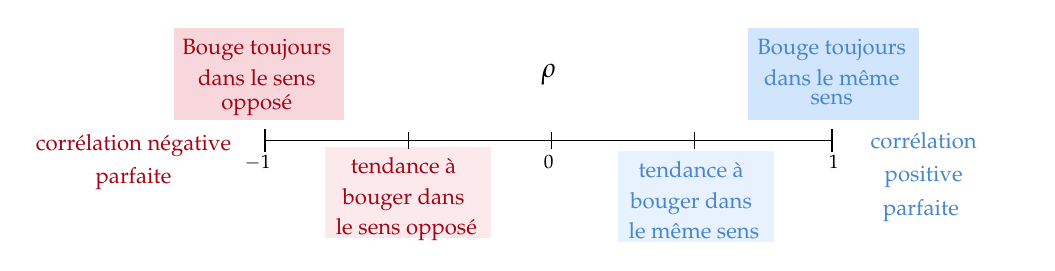
\begin{tikzpicture}[x=0.75pt,y=0.75pt,yscale=-1,xscale=1]
%uncomment if require: \path (0,300); %set diagram left start at 0, and has height of 300

%Straight Lines [id:da7855246610174613] 
\draw    (173,70) -- (446.16,70) (242,66) -- (242,74)(311,66) -- (311,74)(380,66) -- (380,74) ;
\draw [shift={(446.16,70)}, rotate = 180] [color={rgb, 255:red, 0; green, 0; blue, 0 }  ][line width=0.75]    (0,5.59) -- (0,-5.59)   ;
\draw [shift={(173,70)}, rotate = 180] [color={rgb, 255:red, 0; green, 0; blue, 0 }  ][line width=0.75]    (0,5.59) -- (0,-5.59)   ;

% Text Node
\draw (162,76) node [anchor=north west][inner sep=0.75pt]  [font=\scriptsize] [align=left] {$\displaystyle -1$};
% Text Node
\draw (443.46,76) node [anchor=north west][inner sep=0.75pt]  [font=\scriptsize] [align=left] {$\displaystyle 1$};
% Text Node
\draw (306.23,76) node [anchor=north west][inner sep=0.75pt]  [font=\scriptsize] [align=left] {$\displaystyle 0$};
% Text Node
\draw  [draw opacity=0][fill={rgb, 255:red, 232; green, 137; blue, 149 }  ,fill opacity=0.34 ]  (129,16) -- (211,16) -- (211,60) -- (129,60) -- cycle  ;
\draw (132,20) node [anchor=north west][inner sep=0.75pt]  [font=\small,color={rgb, 255:red, 163; green, 5; blue, 24 }  ,opacity=1 ] [align=left] {
\footnotesize\textcolor[rgb]{0.64,0.02,0.09}{\shortstack[c]{Bouge toujours\\ dans le sens\\ opposé}}};
% Text Node
\draw  [draw opacity=0][fill={rgb, 255:red, 182; green, 214; blue, 252 }  ,fill opacity=0.63 ]  (406,16) -- (488,16) -- (488,60) -- (406,60) -- cycle  ;
\draw (409,20) node [anchor=north west][inner sep=0.75pt]  [font=\small,color={rgb, 255:red, 163; green, 5; blue, 24 }  ,opacity=1 ] [align=left] {
\footnotesize\textcolor[rgb]{0.28,0.52,0.8}{\shortstack[c]{Bouge toujours\\ dans le même\\ sens}}
};

% Text Node
\draw (440.5,65) node [anchor=north west][inner sep=0.75pt]  [color={rgb, 255:red, 163; green, 5; blue, 24 }  ,opacity=1 ] [align=left] {\begin{minipage}[lt]{73.02180000000001pt}\setlength\topsep{0pt}
\begin{center}
{\footnotesize \textcolor[rgb]{0.28,0.52,0.8}{corrélation}}\\{\footnotesize \textcolor[rgb]{0.28,0.52,0.8}{positive}}\\{\footnotesize \textcolor[rgb]{0.28,0.52,0.8}{parfaite }}
\end{center}

\end{minipage}};
% Text Node
\draw (59,66) node [anchor=north west][inner sep=0.75pt]  [color={rgb, 255:red, 163; green, 5; blue, 24 }  ,opacity=1 ] [align=left] {\begin{minipage}[lt]{76.20964000000001pt}\setlength\topsep{0pt}
\begin{center}
{\footnotesize \textcolor[rgb]{0.64,0.02,0.09}{corrélation négative }}\\{\footnotesize \textcolor[rgb]{0.64,0.02,0.09}{parfaite }}
\end{center}

\end{minipage}};
% Text Node
\draw  [draw opacity=0][fill={rgb, 255:red, 232; green, 137; blue, 149 }  ,fill opacity=0.19 ]  (202.17,73) -- (282.17,73) -- (282.17,117) -- (202.17,117) -- cycle  ;
\draw (205.17,77) node [anchor=north west][inner sep=0.75pt]  [font=\small,color={rgb, 255:red, 163; green, 5; blue, 24 }  ,opacity=1 ] [align=left] {\begin{minipage}[lt]{52.126216pt}\setlength\topsep{0pt}
\begin{center}
{\footnotesize \textcolor[rgb]{0.64,0.02,0.09}{tendance à }}\\{\footnotesize \textcolor[rgb]{0.64,0.02,0.09}{bouger dans }}\\{\footnotesize \textcolor[rgb]{0.64,0.02,0.09}{le sens opposé}}
\end{center}

\end{minipage}};
% Text Node
\draw  [draw opacity=0][fill={rgb, 255:red, 182; green, 214; blue, 252 }  ,fill opacity=0.32 ]  (343.17,75) -- (418.17,75) -- (418.17,119) -- (343.17,119) -- cycle  ;
\draw (346.17,79) node [anchor=north west][inner sep=0.75pt]  [font=\small,color={rgb, 255:red, 163; green, 5; blue, 24 }  ,opacity=1 ] [align=left] {\begin{minipage}[lt]{48.43585600000001pt}\setlength\topsep{0pt}
\begin{center}
{\footnotesize \textcolor[rgb]{0.28,0.52,0.8}{tendance à }}\\{\footnotesize \textcolor[rgb]{0.28,0.52,0.8}{bouger dans }}\\{\footnotesize \textcolor[rgb]{0.28,0.52,0.8}{le même sens}}
\end{center}

\end{minipage}};
% Text Node
\draw (305,32) node [anchor=north west][inner sep=0.75pt]   [align=left] {$\displaystyle \rho $};


\end{tikzpicture}
\end{center}

\tcbline

\begin{itemize}
	\item	L'avantage de la corrélation est qu'elle n'est pas sur l'échelle des variables mesurées.
\end{itemize}
\end{definitionNOHFILL}

Pour un portefeuille composé de 2 actifs, \lfbox[formula]{$\sigma_{p}^{2}	=	w_{1}^{2}\sigma_{R_{1}}^{2} + w_{2}^{2}\sigma_{R_{2}}^{2} + 2w_{1}w_{2}\rho_{1, 2}\sigma_{R_{1}}\sigma_{R_{2}}$}.\\
Dans le cas plus général : 
\begin{align*}
	\text{Var}(R_{p})	
	&=	\text{Cov}(R_{p}, R_{p})
	=	\sumz{n}{i	=	1}\sumz{n}{j	=	1} w_{i}w_{j} \text{Cov}(R_{i}, R_{j})
\end{align*}


\columnbreak
\subsection{Diversification}
\begin{definitionNOHFILLprop}[Types de risque]
\begin{description}
	\item[Risque systématique]	Risque inhérent au marché. 
		\begin{itemize}
		\item	Alias, risque du marché ou \og \textit{undiversifiable risk} \fg{} en anglais ;
		\item	Par exemple, les fluctuations due aux cycles économiques.
		\end{itemize}
	\item[Risque non-systématique]	Risque inhérent à une compagnie, ou industrie, particulière.
		\begin{itemize}
		\item	Alias, risque indépendant ou \og \textit{diversifiable risk} \fg{} en anglais ;
		\item	Par exemple, la fluctuation de la valeur d'un titre découlant de nouvelles qui y sont spécifiques (p. ex., le prix de l'action d'Apple baisse de 3\$ après qu'ils annoncent une mise à pied d'employés).
		\end{itemize}
	\item[Diversification]	Réduis le risque relié au portefeuille d'une compagnie en agrégeant les fluctuations \underline{non systématiques}. 
\end{description}
\end{definitionNOHFILLprop}

\begin{rappel_enhanced}[Raccourci Bernoulli]
Soit la probabilité $p$ de $a$ et la probabilité $1 - p$ de $b$.\\
Alors, la variance est \lfbox[formula]{$(b - a)^{2}p(1 - p)$}.
\end{rappel_enhanced}

Soit :
\begin{itemize}
	\item	un portefeuille de $n$ actions;
	\item	le poids de chaque action \lfbox[conditions]{$x_{i}	=	\frac{1}{n}$}.
\end{itemize}

La matrice de covariance du portefeuille est : 
\begin{align*}
	\begin{bmatrix}
	\sigma_{1, 1}	&	\sigma_{1, 2}	&	\hdots	&	\sigma_{1, n}	\\
	\sigma_{2, 1}	&	\sigma_{2, 2}	&	\hdots	&	\sigma_{2, n}	\\
	\vdots	&	\vdots	&	\ddots	&	\vdots	\\
	\sigma_{n, 1}	&	\sigma_{n, 2}	&	\hdots	&	\sigma_{n, n}	
	\end{bmatrix}
\end{align*}
\begin{itemize}
	\item	Il s'ensuit qu'elle a $n^{2}$ termes dont $n$ de variance et $n^{2}	-	n$ de covariance dont la moitié ($\frac{n^{2} - n}{2}$) sont uniques.
\end{itemize}

On peut exprimer :
	\setlength{\mathindent}{-1cm}
	\begin{align*}
	\text{Var}(R_{p})	
	&=	\frac{1}{n} \times \underbrace{\left(\text{variance moyenne}\right)}_{\small{\shortstack{risque systémique\\ diversifiable}}} + \left(1 - \frac{1}{n}\right)  \times  \underbrace{\left(\text{covariance moyenne}\right)}_{\small{\shortstack{risque \textit{non} systémique\\ \textit{non} diversifiable}}}
	\end{align*}
	\setlength{\mathindent}{1cm}

\begin{itemize}
	\item	On déduit que $\text{Var}(R_{p}) \underset{n\rightarrow \infty}{\longrightarrow} \shortstack{covariance moyenne (entre les actions)}$.
\end{itemize}


\columnbreak
\subsection{Mean-Variance Portfolio Theory}
\subsubsection{Portefeuilles efficients}
\begin{definitionNOHFILL}[Analyse de portefeuille moyenne-variance]
L'analyse de portefeuille moyenne-variance pose que les investisseurs peuvent évaluer les caractéristiques du risque-rendement d'un investissement avec les rendements espérés, les variances et les corrélations des actifs.
\end{definitionNOHFILL}

\begin{conceptgen}{Hypothèses sous-jacentes à l'analyse de portefeuille moyenne-variance}
\begin{enumerate}
	\item	Tous les investisseurs ont une aversion au risque.
	\item	Les rendements espérés, les variances et les covariances des actifs sont supposés connus.
	\item	Pour déterminer un portefeuille optimal, les investisseurs n'ont qu'à connaitre les rendements espérés, les variances et les covariances des rendements.
	\item	Il n'y a aucun frais de transactions, ni de taxes.
\end{enumerate}
\end{conceptgen}

Pour trouver des portefeuilles efficients, on utilise le diagramme de moyenne-variance. Ce diagramme fait varier les proportions $x_{A}$ et $x_{B}$ investis dans deux actifs $A$ et $B$ :
\begin{center}

\tikzset{every picture/.style={line width=0.75pt}} %set default line width to 0.75pt        

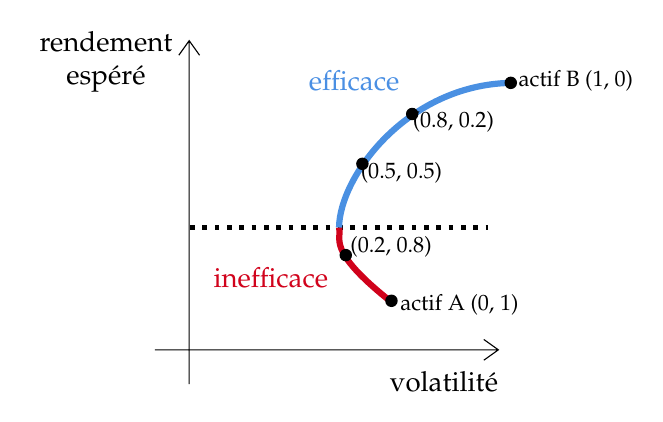
\begin{tikzpicture}[x=0.75pt,y=0.75pt,yscale=-1,xscale=1]
%uncomment if require: \path (0,208); %set diagram left start at 0, and has height of 208

%Shape: Axis 2D [id:dp4877478511835136] 
\draw  (102,180.95) -- (267.5,180.95)(118.55,32) -- (118.55,197.5) (260.5,175.95) -- (267.5,180.95) -- (260.5,185.95) (113.55,39) -- (118.55,32) -- (123.55,39)  ;
%Straight Lines [id:da5292878918548434] 
\draw [line width=1.5]  [dash pattern={on 1.69pt off 2.76pt}]  (119,122) -- (262.5,122) ;
%Curve Lines [id:da7544269338190221] 
\draw [color={rgb, 255:red, 208; green, 2; blue, 27 }  ,draw opacity=1 ][line width=2.25]    (190.75,122) .. controls (192.5,127.32) and (183.5,132.32) .. (216.5,158.32) ;
%Curve Lines [id:da9655156149195883] 
\draw [color={rgb, 255:red, 74; green, 144; blue, 226 }  ,draw opacity=1 ][line width=2.25]    (273.5,52.32) .. controls (223.5,53.32) and (191,97.5) .. (190.75,122) ;
%Shape: Circle [id:dp775694287030839] 
\draw  [draw opacity=0][fill={rgb, 255:red, 0; green, 0; blue, 0 }  ,fill opacity=1 ] (191,135.32) .. controls (191,133.67) and (192.34,132.32) .. (194,132.32) .. controls (195.66,132.32) and (197,133.67) .. (197,135.32) .. controls (197,136.98) and (195.66,138.32) .. (194,138.32) .. controls (192.34,138.32) and (191,136.98) .. (191,135.32) -- cycle ;
%Shape: Circle [id:dp9336389306192374] 
\draw  [draw opacity=0][fill={rgb, 255:red, 0; green, 0; blue, 0 }  ,fill opacity=1 ] (213,157.32) .. controls (213,155.67) and (214.34,154.32) .. (216,154.32) .. controls (217.66,154.32) and (219,155.67) .. (219,157.32) .. controls (219,158.98) and (217.66,160.32) .. (216,160.32) .. controls (214.34,160.32) and (213,158.98) .. (213,157.32) -- cycle ;
%Shape: Circle [id:dp4743935385951963] 
\draw  [draw opacity=0][fill={rgb, 255:red, 0; green, 0; blue, 0 }  ,fill opacity=1 ] (199,91.32) .. controls (199,89.67) and (200.34,88.32) .. (202,88.32) .. controls (203.66,88.32) and (205,89.67) .. (205,91.32) .. controls (205,92.98) and (203.66,94.32) .. (202,94.32) .. controls (200.34,94.32) and (199,92.98) .. (199,91.32) -- cycle ;
%Shape: Circle [id:dp37018445621976737] 
\draw  [draw opacity=0][fill={rgb, 255:red, 0; green, 0; blue, 0 }  ,fill opacity=1 ] (223,67.32) .. controls (223,65.67) and (224.34,64.32) .. (226,64.32) .. controls (227.66,64.32) and (229,65.67) .. (229,67.32) .. controls (229,68.98) and (227.66,70.32) .. (226,70.32) .. controls (224.34,70.32) and (223,68.98) .. (223,67.32) -- cycle ;
%Shape: Circle [id:dp9284342964070993] 
\draw  [draw opacity=0][fill={rgb, 255:red, 0; green, 0; blue, 0 }  ,fill opacity=1 ] (270.5,52.32) .. controls (270.5,50.67) and (271.84,49.32) .. (273.5,49.32) .. controls (275.16,49.32) and (276.5,50.67) .. (276.5,52.32) .. controls (276.5,53.98) and (275.16,55.32) .. (273.5,55.32) .. controls (271.84,55.32) and (270.5,53.98) .. (270.5,52.32) -- cycle ;

% Text Node
\draw (214,190) node [anchor=north west][inner sep=0.75pt]   [align=left] {volatilité};
% Text Node
\draw (41,26) node [anchor=north west][inner sep=0.75pt]   [align=left] {\begin{minipage}[lt]{54.3235pt}\setlength\topsep{0pt}
\begin{center}
rendement \\espéré
\end{center}

\end{minipage}};
% Text Node
\draw (175,45) node [anchor=north west][inner sep=0.75pt]   [align=left] {\textcolor[rgb]{0.29,0.56,0.89}{efficace}};
% Text Node
\draw (129,140) node [anchor=north west][inner sep=0.75pt]   [align=left] {\textcolor[rgb]{0.82,0.01,0.11}{inefficace}};
% Text Node
\draw (276,45) node [anchor=north west][inner sep=0.75pt]  [font=\footnotesize] [align=left] {actif B (1, 0)};
% Text Node
\draw (219,153) node [anchor=north west][inner sep=0.75pt]  [font=\footnotesize] [align=left] {actif A (0, 1)};
% Text Node
\draw (200,89.32) node [anchor=north west][inner sep=0.75pt]  [font=\footnotesize] [align=left] { (0.5, 0.5)};
% Text Node
\draw (225,65) node [anchor=north west][inner sep=0.75pt]  [font=\footnotesize] [align=left] { (0.8, 0.2)};
% Text Node
\draw (195,125) node [anchor=north west][inner sep=0.75pt]  [font=\footnotesize] [align=left] { (0.2, 0.8)};


\end{tikzpicture}

\end{center}

Un portefeuille est :
\begin{description}
	\item[efficient]	Si pour un niveau donné de volatilité, il offre le meilleur rendement espéré.
	\item[inefficient]	Si pour un niveau donné de volatilité, il est possible de trouver un meilleur rendement espéré.
\end{description}

\begin{definitionNOHFILL}[Frontière efficiente]
Courbe des portefeuilles maximisant le rendement espéré pour un niveau de volatilité donné. \\

Selon son niveau de risque, un investisseur choisit des proportions parmi ceux qui sont sur la frontière efficiente. Par exemple, un investisseur avec une tolérance au risque élevée pourrait choisir un portefeuille avec une plus grande volatilité pour avoir un rendement espéré plus élevé.
\end{definitionNOHFILL}


La corrélation entre actifs peut impacter la frontière, par exemple si l'on investi dans 2 actifs : 
\begin{center}
\tikzset{every picture/.style={line width=0.75pt}} %set default line width to 0.75pt        

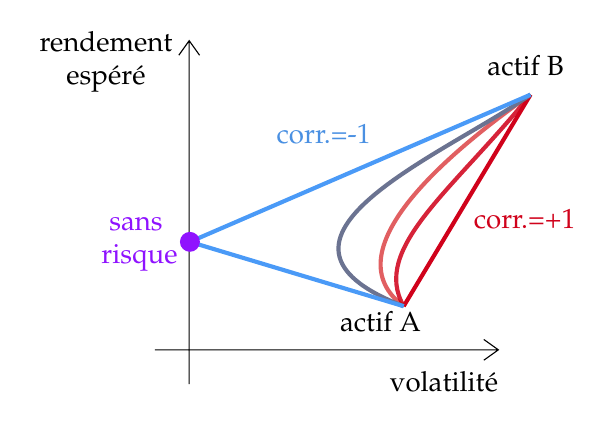
\begin{tikzpicture}[x=0.75pt,y=0.75pt,yscale=-1,xscale=1]
%uncomment if require: \path (0,300); %set diagram left start at 0, and has height of 300

%Shape: Axis 2D [id:dp36472036740726677] 
\draw  (102,180.95) -- (267.5,180.95)(118.55,32) -- (118.55,197.5) (260.5,175.95) -- (267.5,180.95) -- (260.5,185.95) (113.55,39) -- (118.55,32) -- (123.55,39)  ;
%Straight Lines [id:da06881977667489858] 
\draw [color={rgb, 255:red, 208; green, 2; blue, 27 }  ,draw opacity=1 ][line width=1.5]    (283,58) -- (221.9,159.93) ;
%Curve Lines [id:da19740884975223993] 
\draw [color={rgb, 255:red, 208; green, 2; blue, 27 }  ,draw opacity=0.87 ][line width=1.5]    (221.9,159.93) .. controls (205.9,131.93) and (245.9,103.93) .. (283,58) ;
%Curve Lines [id:da42806367647793087] 
\draw [color={rgb, 255:red, 208; green, 2; blue, 5 }  ,draw opacity=0.63 ][line width=1.5]    (221.9,159.93) .. controls (186.9,133.93) and (241.9,86.93) .. (283,58) ;
%Curve Lines [id:da8219225169519757] 
\draw [color={rgb, 255:red, 107; green, 115; blue, 145 }  ,draw opacity=1 ][line width=1.5]    (221.9,159.93) .. controls (138.9,127.93) and (241.9,86.93) .. (283,58) ;
%Straight Lines [id:da05456530275003768] 
\draw [color={rgb, 255:red, 74; green, 154; blue, 247 }  ,draw opacity=1 ][line width=1.5]    (283,58) -- (118.9,128.93) ;
%Straight Lines [id:da2204623788548825] 
\draw [color={rgb, 255:red, 74; green, 154; blue, 247 }  ,draw opacity=1 ][line width=1.5]    (221.9,159.93) -- (118.9,128.93) ;
%Shape: Circle [id:dp08392787883452146] 
\draw  [draw opacity=0][fill={rgb, 255:red, 144; green, 19; blue, 254 }  ,fill opacity=1 ] (114.1,128.93) .. controls (114.1,126.27) and (116.25,124.13) .. (118.9,124.13) .. controls (121.55,124.13) and (123.7,126.27) .. (123.7,128.93) .. controls (123.7,131.58) and (121.55,133.72) .. (118.9,133.72) .. controls (116.25,133.72) and (114.1,131.58) .. (114.1,128.93) -- cycle ;

% Text Node
\draw (214,190) node [anchor=north west][inner sep=0.75pt]   [align=left] {volatilité};
% Text Node
\draw (41,26) node [anchor=north west][inner sep=0.75pt]   [align=left] {\begin{minipage}[lt]{54.3235pt}\setlength\topsep{0pt}
\begin{center}
rendement \\espéré
\end{center}

\end{minipage}};
% Text Node
\draw (190,161) node [anchor=north west][inner sep=0.75pt]   [align=left] {actif A};
% Text Node
\draw (261,38) node [anchor=north west][inner sep=0.75pt]   [align=left] {actif B};
% Text Node
\draw (254.45,111.96) node [anchor=north west][inner sep=0.75pt]  [color={rgb, 255:red, 208; green, 2; blue, 27 }  ,opacity=1 ] [align=left] {corr.=+1};
% Text Node
\draw (159.45,70.96) node [anchor=north west][inner sep=0.75pt]  [color={rgb, 255:red, 74; green, 144; blue, 226 }  ,opacity=1 ] [align=left] {corr.=-1};
% Text Node
\draw (73,116) node [anchor=north west][inner sep=0.75pt]   [align=left] {\begin{minipage}[lt]{30.5065pt}\setlength\topsep{0pt}
\begin{center}
\textcolor[rgb]{0.56,0.07,1}{sans }\\\textcolor[rgb]{0.56,0.07,1}{risque}
\end{center}

\end{minipage}};


\end{tikzpicture}
\end{center}

Pour un portefeuille composé des actifs $A$ et $B$, lorsque :
\begin{description}
	\item[$\rho_{B, W} = 1$]	la volatilité du portefeuille est maximisée ;
		\begin{itemize}
		\item	Dans ce cas-ci, la volatilité du portefeuille équivaut à la moyenne pondérée de la volatilité des actifs.
		\item	Par exemple, pour un portefeuille composé de deux actifs $A$ et $B$ :
			\begin{align*}
					\sigma_{P}
					&=	\sqrt{w_{A}^{2} \sigma_{A}^{2} + w_{B}^{2} \sigma_{B}^{2} + 2 w_{A} w_{B} (1) \sigma_{A} \sigma_{B}}	\\
					&=	\sqrt{(w_{A} \sigma_{A} + w_{B} \sigma_{B})^{2}}	\\
					&=	w_{A} \sigma_{A} + w_{B} \sigma_{B}
			\end{align*}
		\end{itemize}
	\item[$\rho_{B, W} < 1$]	la volatilité du portefeuille est inférieure à la volatilité pondérée pondérée ;
		\begin{itemize}
		\item	Il s'ensuit que plus la corrélation est faible, plus il est avantageux de diversifier le portefeuille car cela réduit davantage la volatilité ;
		\item	Si deux actifs sont parfaitement corrélés, diversifier ne change pas la volatilité et il n'y a aucun avantage à le faire.
		\end{itemize}
	\item[$\rho_{B, W} = -1$]	On peut construire un portefeuille \textcolor{amethyst}{sans risque}.
\end{description}

Investir un montant négatif dans une action équivaut à un \og \textit{short-sell} \fg{} (vente à découvert) et la frontière est rallongée :
\begin{center}
\tikzset{every picture/.style={line width=0.75pt}} %set default line width to 0.75pt        

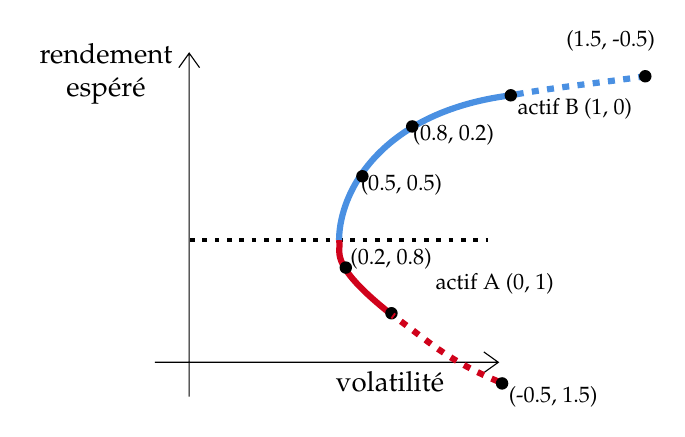
\begin{tikzpicture}[x=0.75pt,y=0.75pt,yscale=-1,xscale=1]
%uncomment if require: \path (0,208); %set diagram left start at 0, and has height of 208

%Curve Lines [id:da126524382447448] 
\draw [color={rgb, 255:red, 74; green, 144; blue, 226 }  ,draw opacity=1 ][line width=2.25]  [dash pattern={on 2.53pt off 3.02pt}]  (338.3,43.13) .. controls (317.3,46.32) and (296.3,48.13) .. (273.5,52.32) ;
%Shape: Axis 2D [id:dp6673318093332545] 
\draw  (102,180.95) -- (267.5,180.95)(118.55,32) -- (118.55,197.5) (260.5,175.95) -- (267.5,180.95) -- (260.5,185.95) (113.55,39) -- (118.55,32) -- (123.55,39)  ;
%Straight Lines [id:da2261641715581777] 
\draw [line width=1.5]  [dash pattern={on 1.69pt off 2.76pt}]  (119,122) -- (262.5,122) ;
%Curve Lines [id:da9106576884133932] 
\draw [color={rgb, 255:red, 208; green, 2; blue, 27 }  ,draw opacity=1 ][line width=2.25]    (190.75,122) .. controls (192.5,127.32) and (183.5,132.32) .. (216.5,158.32) ;
%Curve Lines [id:da05124936898207322] 
\draw [color={rgb, 255:red, 74; green, 144; blue, 226 }  ,draw opacity=1 ][line width=2.25]    (273.5,52.32) .. controls (212.3,60.13) and (191,97.5) .. (190.75,122) ;
%Shape: Circle [id:dp16470704138236059] 
\draw  [draw opacity=0][fill={rgb, 255:red, 0; green, 0; blue, 0 }  ,fill opacity=1 ] (191,135.32) .. controls (191,133.67) and (192.34,132.32) .. (194,132.32) .. controls (195.66,132.32) and (197,133.67) .. (197,135.32) .. controls (197,136.98) and (195.66,138.32) .. (194,138.32) .. controls (192.34,138.32) and (191,136.98) .. (191,135.32) -- cycle ;
%Shape: Circle [id:dp7175051647262234] 
\draw  [draw opacity=0][fill={rgb, 255:red, 0; green, 0; blue, 0 }  ,fill opacity=1 ] (213,157.32) .. controls (213,155.67) and (214.34,154.32) .. (216,154.32) .. controls (217.66,154.32) and (219,155.67) .. (219,157.32) .. controls (219,158.98) and (217.66,160.32) .. (216,160.32) .. controls (214.34,160.32) and (213,158.98) .. (213,157.32) -- cycle ;
%Shape: Circle [id:dp3193182704177373] 
\draw  [draw opacity=0][fill={rgb, 255:red, 0; green, 0; blue, 0 }  ,fill opacity=1 ] (199,91.32) .. controls (199,89.67) and (200.34,88.32) .. (202,88.32) .. controls (203.66,88.32) and (205,89.67) .. (205,91.32) .. controls (205,92.98) and (203.66,94.32) .. (202,94.32) .. controls (200.34,94.32) and (199,92.98) .. (199,91.32) -- cycle ;
%Shape: Circle [id:dp2900673953428521] 
\draw  [draw opacity=0][fill={rgb, 255:red, 0; green, 0; blue, 0 }  ,fill opacity=1 ] (223,67.32) .. controls (223,65.67) and (224.34,64.32) .. (226,64.32) .. controls (227.66,64.32) and (229,65.67) .. (229,67.32) .. controls (229,68.98) and (227.66,70.32) .. (226,70.32) .. controls (224.34,70.32) and (223,68.98) .. (223,67.32) -- cycle ;
%Shape: Circle [id:dp10862219342683344] 
\draw  [draw opacity=0][fill={rgb, 255:red, 0; green, 0; blue, 0 }  ,fill opacity=1 ] (270.5,52.32) .. controls (270.5,50.67) and (271.84,49.32) .. (273.5,49.32) .. controls (275.16,49.32) and (276.5,50.67) .. (276.5,52.32) .. controls (276.5,53.98) and (275.16,55.32) .. (273.5,55.32) .. controls (271.84,55.32) and (270.5,53.98) .. (270.5,52.32) -- cycle ;
%Curve Lines [id:da600668274682344] 
\draw [color={rgb, 255:red, 208; green, 2; blue, 27 }  ,draw opacity=1 ][line width=2.25]  [dash pattern={on 2.53pt off 3.02pt}]  (267.3,190.13) .. controls (241.3,179.13) and (233.3,170.13) .. (216.5,158.32) ;
%Shape: Circle [id:dp5703950228917769] 
\draw  [draw opacity=0][fill={rgb, 255:red, 0; green, 0; blue, 0 }  ,fill opacity=1 ] (335.3,43.13) .. controls (335.3,41.47) and (336.64,40.13) .. (338.3,40.13) .. controls (339.96,40.13) and (341.3,41.47) .. (341.3,43.13) .. controls (341.3,44.78) and (339.96,46.13) .. (338.3,46.13) .. controls (336.64,46.13) and (335.3,44.78) .. (335.3,43.13) -- cycle ;
%Shape: Circle [id:dp4593909531372147] 
\draw  [draw opacity=0][fill={rgb, 255:red, 0; green, 0; blue, 0 }  ,fill opacity=1 ] (266.3,191.13) .. controls (266.3,189.47) and (267.64,188.13) .. (269.3,188.13) .. controls (270.96,188.13) and (272.3,189.47) .. (272.3,191.13) .. controls (272.3,192.78) and (270.96,194.13) .. (269.3,194.13) .. controls (267.64,194.13) and (266.3,192.78) .. (266.3,191.13) -- cycle ;

% Text Node
\draw (188,184) node [anchor=north west][inner sep=0.75pt]   [align=left] {volatilité};
% Text Node
\draw (41,26) node [anchor=north west][inner sep=0.75pt]   [align=left] {\begin{minipage}[lt]{54.3235pt}\setlength\topsep{0pt}
\begin{center}
rendement \\espéré
\end{center}

\end{minipage}};
% Text Node
\draw (275.5,52.32) node [anchor=north west][inner sep=0.75pt]  [font=\footnotesize] [align=left] {actif B (1, 0)};
% Text Node
\draw (236,137) node [anchor=north west][inner sep=0.75pt]  [font=\footnotesize] [align=left] {actif A (0, 1)};
% Text Node
\draw (200,89.32) node [anchor=north west][inner sep=0.75pt]  [font=\footnotesize] [align=left] { (0.5, 0.5)};
% Text Node
\draw (225,65) node [anchor=north west][inner sep=0.75pt]  [font=\footnotesize] [align=left] { (0.8, 0.2)};
% Text Node
\draw (195,125) node [anchor=north west][inner sep=0.75pt]  [font=\footnotesize] [align=left] { (0.2, 0.8)};
% Text Node
\draw (299,20) node [anchor=north west][inner sep=0.75pt]  [font=\footnotesize] [align=left] { (1.5, -0.5)};
% Text Node
\draw (271.3,191.13) node [anchor=north west][inner sep=0.75pt]  [font=\footnotesize] [align=left] { (-0.5, 1.5)};


\end{tikzpicture}
\end{center}

Diversifier avec plus d'actions (qui ne sont pas parfaitement corrélées) permet une meilleur frontière efficiente :
\begin{center}
\tikzset{every picture/.style={line width=0.75pt}} %set default line width to 0.75pt        

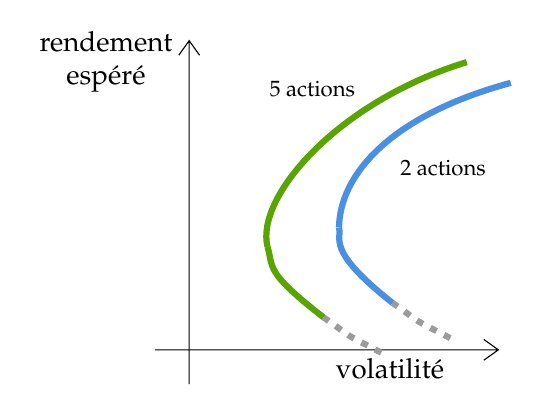
\begin{tikzpicture}[x=0.75pt,y=0.75pt,yscale=-1,xscale=1]
%uncomment if require: \path (0,208); %set diagram left start at 0, and has height of 208

%Shape: Axis 2D [id:dp053135063496398516] 
\draw  (102,180.95) -- (267.5,180.95)(118.55,32) -- (118.55,197.5) (260.5,175.95) -- (267.5,180.95) -- (260.5,185.95) (113.55,39) -- (118.55,32) -- (123.55,39)  ;
%Curve Lines [id:da4116180304977153] 
\draw [color={rgb, 255:red, 74; green, 144; blue, 226 }  ,draw opacity=1 ][line width=2.25]    (190.75,122) .. controls (192.5,127.32) and (183.5,132.32) .. (216.5,158.32) ;
%Curve Lines [id:da8129419759820313] 
\draw [color={rgb, 255:red, 74; green, 144; blue, 226 }  ,draw opacity=1 ][line width=2.25]    (273.5,52.32) .. controls (214.3,68.32) and (191,97.5) .. (190.75,122) ;
%Curve Lines [id:da8791633164216062] 
\draw [color={rgb, 255:red, 155; green, 155; blue, 155 }  ,draw opacity=1 ][line width=2.25]  [dash pattern={on 2.53pt off 3.02pt}]  (244.3,175.32) .. controls (223.3,164.32) and (233.3,170.13) .. (216.5,158.32) ;
%Curve Lines [id:da19605421117215305] 
\draw [color={rgb, 255:red, 88; green, 165; blue, 1 }  ,draw opacity=1 ][line width=2.25]    (156.3,131.32) .. controls (159.3,141.32) and (154.55,143) .. (183.3,165.32) ;
%Curve Lines [id:da771629139304369] 
\draw [color={rgb, 255:red, 88; green, 165; blue, 1 }  ,draw opacity=1 ][line width=2.25]    (252.3,42.32) .. controls (190.1,61.32) and (150.3,107.32) .. (156.3,131.32) ;
%Curve Lines [id:da05631185573198971] 
\draw [color={rgb, 255:red, 155; green, 155; blue, 155 }  ,draw opacity=1 ][line width=2.25]  [dash pattern={on 2.53pt off 3.02pt}]  (211.1,182.32) .. controls (190.1,171.32) and (200.1,177.13) .. (183.3,165.32) ;

% Text Node
\draw (188,184) node [anchor=north west][inner sep=0.75pt]   [align=left] {volatilité};
% Text Node
\draw (41,26) node [anchor=north west][inner sep=0.75pt]   [align=left] {\begin{minipage}[lt]{54.3235pt}\setlength\topsep{0pt}
\begin{center}
rendement \\espéré
\end{center}

\end{minipage}};
% Text Node
\draw (219,88.32) node [anchor=north west][inner sep=0.75pt]  [font=\footnotesize] [align=left] {2 actions};
% Text Node
\draw (156,50.32) node [anchor=north west][inner sep=0.75pt]  [font=\footnotesize] [align=left] {5 actions};


\end{tikzpicture}
\end{center}

Voir \hyperref[sec:MVT-newinv]{la dernière sous-section} pour des détails sur quand qu'il est optimal d'ajouter un nouvel investissement.


\columnbreak
\subsubsection{Combinaisons d'actifs risqués et avec aucun risque}
On peut combiner un portefeuille risqué à un actif sans risque ayant un rendement espéré égale au taux sans risque et une volatilité nulle.\\

Soit un portefeuille composé à $x\%$ d'un portefeuille risqué et à $(1 - x)\%$ d'un actif sans risque.
\begin{distributions}[Notation]
\begin{description}
	\item[$\sigma_{P}$]	volatilité du portefeuille risqué.
		\begin{itemize}
		\item	La volatilité de l'actif sans risque est nulle.
		\end{itemize}
	\item[$r_{f}$]	taux sans risque (alias le rendement espéré) de l'actif sans risque.
%%	------------------------
%%%	NOTES
%%%	+	utiliser [] dans une équation mène à une erreur puisque la liste pense que c'est pour fermer ;
%%%	+	faut utilliser \lbrack et \rbrack à place.
%%%	------------------------
	\item[$\text{E}\lbrack R_{P}\rbrack$]	rendement espéré du portefeuille risqué.
	\item[$\text{E}\lbrack R_{xP}\rbrack$]	rendement espéré d'un portefeuille composé à $x\%$ du portefeuille risqué.
	\item[$\sigma_{xP}$]	volatilité du portefeuille composé à $x\%$ d'un actif risqué
\end{description}
\end{distributions}

On trouve que le rendement espéré du portefeuille est \lfbox[formula]{$\text{E}[R_{xP}]	=	r_{f} + x(\text{E}[R_{P}] - r_{f})$} et que la volatilité est \lfbox[formula]{$\sigma_{xP}	=	x\sigma_{P}$}. 

\begin{definitionNOHFILL}[Droite d'allocation du capital]
%%	------------------------
%%%	NOTES
%%%	+	Clarifier cette définition.
%%%	------------------------
La droite d'allocation du capital (AC) décrit les rendements espérés et volatilités possibles des différentes combinaisons d'un portefeuille risqué et d'un actif sans risque :
\begin{center}
\tikzset{every picture/.style={line width=0.75pt}} %set default line width to 0.75pt        

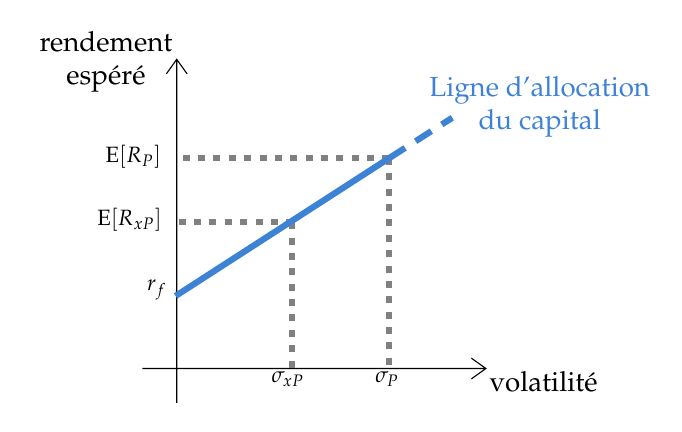
\begin{tikzpicture}[x=0.75pt,y=0.75pt,yscale=-1,xscale=1]
%uncomment if require: \path (0,208); %set diagram left start at 0, and has height of 208

%Shape: Axis 2D [id:dp16704807941155386] 
\draw  (102,180.95) -- (267.5,180.95)(118.55,32) -- (118.55,197.5) (260.5,175.95) -- (267.5,180.95) -- (260.5,185.95) (113.55,39) -- (118.55,32) -- (123.55,39)  ;
%Straight Lines [id:da9724090132301113] 
\draw [color={rgb, 255:red, 128; green, 128; blue, 128 }  ,draw opacity=1 ][line width=2.25]  [dash pattern={on 2.53pt off 3.02pt}]  (174,110.52) -- (174,183) ;
%Straight Lines [id:da6016442902359609] 
\draw [color={rgb, 255:red, 128; green, 128; blue, 128 }  ,draw opacity=1 ][line width=2.25]  [dash pattern={on 2.53pt off 3.02pt}]  (221,79.52) -- (221,183) ;
%Straight Lines [id:da3065084885013789] 
\draw [color={rgb, 255:red, 128; green, 128; blue, 128 }  ,draw opacity=1 ][line width=2.25]  [dash pattern={on 2.53pt off 3.02pt}]  (221,79.52) -- (120.5,79.52) ;
%Straight Lines [id:da5676477547539422] 
\draw [color={rgb, 255:red, 128; green, 128; blue, 128 }  ,draw opacity=1 ][line width=2.25]  [dash pattern={on 2.53pt off 3.02pt}]  (119.5,110.52) -- (174,110.52) ;
%Straight Lines [id:da004443162701488479] 
\draw [color={rgb, 255:red, 61; green, 131; blue, 213 }  ,draw opacity=1 ][line width=2.25]    (221,79.52) -- (118,146) ;
%Straight Lines [id:da2382628136252254] 
\draw [color={rgb, 255:red, 61; green, 131; blue, 213 }  ,draw opacity=1 ][line width=2.25]  [dash pattern={on 6.75pt off 4.5pt}]  (221,79.52) -- (251.3,60.13) ;

% Text Node
\draw (268,181) node [anchor=north west][inner sep=0.75pt]   [align=left] {volatilité};
% Text Node
\draw (47,17) node [anchor=north west][inner sep=0.75pt]   [align=left] {\begin{minipage}[lt]{54.3235pt}\setlength\topsep{0pt}
\begin{center}
rendement \\espéré
\end{center}

\end{minipage}};
% Text Node
\draw (83,72.32) node [anchor=north west][inner sep=0.75pt]  [font=\footnotesize] [align=left] {$\displaystyle \text{E}[ R_{P}]$};
% Text Node
\draw (79,102.32) node [anchor=north west][inner sep=0.75pt]  [font=\footnotesize] [align=left] {$\displaystyle \text{E}[ R_{xP}]$};
% Text Node
\draw (163,181) node [anchor=north west][inner sep=0.75pt]  [font=\footnotesize] [align=left] {$\displaystyle \sigma _{xP}$};
% Text Node
\draw (213,181) node [anchor=north west][inner sep=0.75pt]  [font=\footnotesize] [align=left] {$\displaystyle \sigma _{P}$};
% Text Node
\draw (103,137) node [anchor=north west][inner sep=0.75pt]  [font=\footnotesize] [align=left] {$\displaystyle r_{f}$};
% Text Node
\draw (238,39) node [anchor=north west][inner sep=0.75pt]   [align=left] {\begin{minipage}[lt]{81.23484pt}\setlength\topsep{0pt}
\begin{center}
\textcolor[rgb]{0.24,0.51,0.84}{Ligne d'allocation}\\\textcolor[rgb]{0.24,0.51,0.84}{du capital}
\end{center}

\end{minipage}};


\end{tikzpicture}
\end{center}

On trouve \lfbox[conditions]{$x	=	\frac{\sigma_{xP}}{\sigma_{P}}$} avec l'équation pour la volatilité du portefeuille puis on le substitue dans l'équation du rendement pour trouver :  \lfbox[formula]{$\text{E}[R_{xP}]	=	r_{f} + \sigma_{xP} \frac{\text{E}[R_{P}]	-	r_{f}}{\sigma_{P}}$}.

\begin{itemize}
	\item	En anglais, \og \textit{capital allocation line (CAL)} \fg{} ;
	\item	La pente de la droite d'AC représente le rendement additionnel disponible par incrément d'une unité de risque et équivaut au \textit{\textbf{ratio de Sharpe}}.
\end{itemize}
\end{definitionNOHFILL}

\begin{definitionNOHFILLsub}[Achat d'actions sur marge]
Emprunter au taux sans risque puis acheter des actions risqués.
\begin{itemize}
	\item	En anglais, \og \textit{buying stocks on margin} \fg{};
	\item	On peut aussi dire qu'on achète les actions avec un \textbf{effet de levier}.
\end{itemize}
\end{definitionNOHFILLsub}

\begin{definitionNOHFILLsub}[Portefeuille avec levier]
Portefeuille qui consiste d'une position courte sur l'actif sans risque.
\begin{itemize}
	\item	En anglais, \og \textit{levered portfolio} \fg{} ;
	\item	Visuellement, ceci équivaut au pointillé de la droite d'AC ;
	\item	Il s'ensuit qu'une vente à découvert implique un rendement \textit{et} une volatilité plus élevée.
\end{itemize}

\begin{formula}{Exemple de vente à découvert}
Par exemple, je souhaite investir dans un portefeuille de 30\$ avec 10\$.\\
Alors, $x	=	300\%	=	3$ puisque la portion risquée du portefeuille équivaut à 300\% de mon investissement initial.
\end{formula}
\end{definitionNOHFILLsub}


Avec la droite de l'AC et la frontière efficiente, on peut trouver le \textbf{portefeuille risqué optimal} $P$ :
\begin{center}
\tikzset{every picture/.style={line width=0.75pt}} %set default line width to 0.75pt        

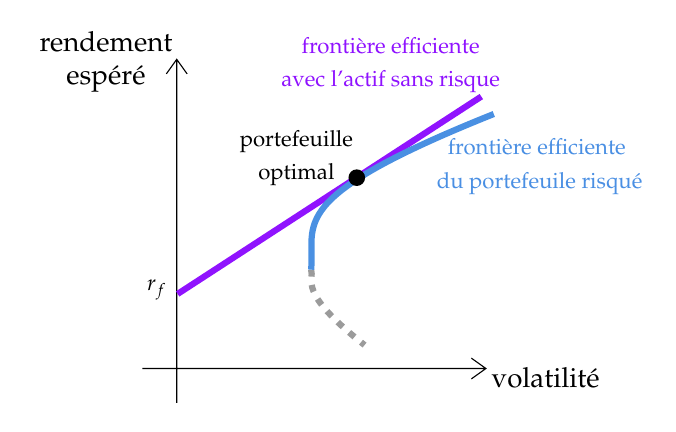
\begin{tikzpicture}[x=0.75pt,y=0.75pt,yscale=-1,xscale=1]
%uncomment if require: \path (0,208); %set diagram left start at 0, and has height of 208

%Shape: Axis 2D [id:dp6485885315666768] 
\draw  (102,180.95) -- (267.5,180.95)(118.55,32) -- (118.55,197.5) (260.5,175.95) -- (267.5,180.95) -- (260.5,185.95) (113.55,39) -- (118.55,32) -- (123.55,39)  ;
%Straight Lines [id:da6187697978759195] 
\draw [color={rgb, 255:red, 144; green, 19; blue, 254 }  ,draw opacity=1 ][line width=2.25]    (265.3,49.92) -- (119,145) ;
%Curve Lines [id:da32863019282893036] 
\draw [color={rgb, 255:red, 155; green, 155; blue, 155 }  ,draw opacity=1 ][line width=2.25]  [dash pattern={on 2.53pt off 3.02pt}]  (183.3,133.32) .. controls (185.05,138.65) and (176.05,143.65) .. (209.05,169.65) ;
%Curve Lines [id:da8344007314232385] 
\draw [color={rgb, 255:red, 74; green, 144; blue, 226 }  ,draw opacity=1 ][line width=2.25]    (271.3,58.32) .. controls (169.3,99.13) and (185.3,111.13) .. (183.3,133.32) ;
%Shape: Circle [id:dp8762352669922273] 
\draw  [draw opacity=0][fill={rgb, 255:red, 0; green, 0; blue, 0 }  ,fill opacity=1 ] (201.3,89) .. controls (201.3,86.79) and (203.09,85) .. (205.3,85) .. controls (207.51,85) and (209.3,86.79) .. (209.3,89) .. controls (209.3,91.21) and (207.51,93) .. (205.3,93) .. controls (203.09,93) and (201.3,91.21) .. (201.3,89) -- cycle ;

% Text Node
\draw (269,179) node [anchor=north west][inner sep=0.75pt]   [align=left] {volatilité};
% Text Node
\draw (47,17) node [anchor=north west][inner sep=0.75pt]   [align=left] {\begin{minipage}[lt]{54.3235pt}\setlength\topsep{0pt}
\begin{center}
rendement \\espéré
\end{center}

\end{minipage}};
% Text Node
\draw (103,137) node [anchor=north west][inner sep=0.75pt]  [font=\footnotesize] [align=left] {$\displaystyle r_{f}$};
% Text Node
\draw (164,20) node [anchor=north west][inner sep=0.75pt]   [align=left] {\begin{minipage}[lt]{84.558pt}\setlength\topsep{0pt}
\begin{center}
{\footnotesize \textcolor[rgb]{0.56,0.07,1}{frontière efficiente}}\\{\footnotesize \textcolor[rgb]{0.56,0.07,1}{avec l'actif sans risque}}
\end{center}

\end{minipage}};
% Text Node
\draw (241,69) node [anchor=north west][inner sep=0.75pt]   [align=left] {\begin{minipage}[lt]{76.67pt}\setlength\topsep{0pt}
\begin{center}
\textcolor[rgb]{0.29,0.56,0.89}{{\footnotesize frontière efficiente }}\\\textcolor[rgb]{0.29,0.56,0.89}{{\footnotesize du portefeuile risqué}}
\end{center}

\end{minipage}};
% Text Node
\draw (145,65) node [anchor=north west][inner sep=0.75pt]   [align=left] {\begin{minipage}[lt]{44.914pt}\setlength\topsep{0pt}
\begin{center}
{\footnotesize portefeuille }\\{\footnotesize optimal}
\end{center}

\end{minipage}};


\end{tikzpicture}
\end{center}

\begin{itemize}
	\item	On l'appel aussi \textit{le portefeuille efficient} et \textit{le portefeuille tangent} ;
	\item	Ce point correspond au maximum de la pente et donc maximise le ratio de Sharpe.
\end{itemize}


\columnbreak
\subsubsection{Droite du marché des capitaux}
\begin{rappel_enhanced}[Contexte]
Si chaque investisseur a des attentes de rendement espéré, volatilité et corrélation différentes, alors chaque investisseur aura une droite d'AC et un portefeuille risqué optimal différent.\\

Cependant, afin de simplifier l'analyse moyenne-variance on pose habituellement que les investisseurs ont des espérances homogènes et donc qu'ils ont tous la même estimation de la volatilité, de la corrélation et du rendement espéré de titres financiers.
\end{rappel_enhanced}

L'hypothèse que les attentes des investisseurs sont homogènes implique également une même droite d'AC et un même portefeuille optimal pour le marché.

\begin{definitionNOHFILL}[Portefeuille du marché (PM)]
Portefeuille optimal du marché (PM).
\begin{itemize}
	\item	En théorie, il est composé de toutes les actions et tous les titres financiers risqués du marché ;
	\item	En pratique, ceci est impossible et l'on utilise un indice tel que le S\&P 500 ;
	\item	En anglais, \og \textit{market portfolio} \fg{}.
\end{itemize}
\end{definitionNOHFILL}

\begin{definitionNOHFILL}[Droite du marché des capitaux]
Droite d'AC du marché.

\begin{center}
\tikzset{every picture/.style={line width=0.75pt}} %set default line width to 0.75pt        

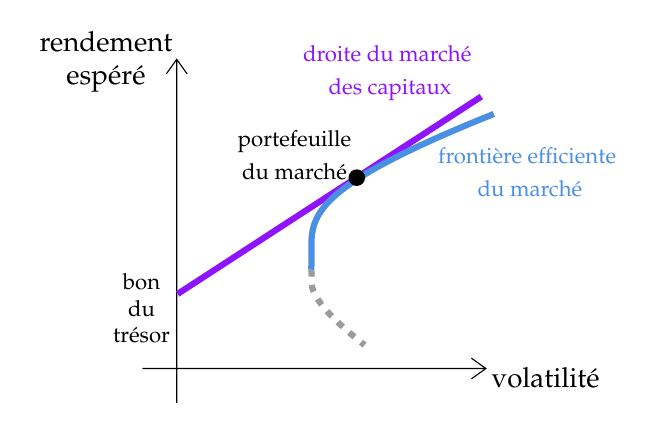
\begin{tikzpicture}[x=0.75pt,y=0.75pt,yscale=-1,xscale=1]
%uncomment if require: \path (0,208); %set diagram left start at 0, and has height of 208

%Shape: Axis 2D [id:dp954299495869529] 
\draw  (102,180.95) -- (267.5,180.95)(118.55,32) -- (118.55,197.5) (260.5,175.95) -- (267.5,180.95) -- (260.5,185.95) (113.55,39) -- (118.55,32) -- (123.55,39)  ;
%Straight Lines [id:da7226226944481302] 
\draw [color={rgb, 255:red, 144; green, 19; blue, 254 }  ,draw opacity=1 ][line width=2.25]    (265.3,49.92) -- (119,145) ;
%Curve Lines [id:da11750654254498083] 
\draw [color={rgb, 255:red, 155; green, 155; blue, 155 }  ,draw opacity=1 ][line width=2.25]  [dash pattern={on 2.53pt off 3.02pt}]  (183.3,133.32) .. controls (185.05,138.65) and (176.05,143.65) .. (209.05,169.65) ;
%Curve Lines [id:da7446996086761495] 
\draw [color={rgb, 255:red, 74; green, 144; blue, 226 }  ,draw opacity=1 ][line width=2.25]    (271.3,58.32) .. controls (169.3,99.13) and (185.3,111.13) .. (183.3,133.32) ;
%Shape: Circle [id:dp2662101856372143] 
\draw  [draw opacity=0][fill={rgb, 255:red, 0; green, 0; blue, 0 }  ,fill opacity=1 ] (201.3,89) .. controls (201.3,86.79) and (203.09,85) .. (205.3,85) .. controls (207.51,85) and (209.3,86.79) .. (209.3,89) .. controls (209.3,91.21) and (207.51,93) .. (205.3,93) .. controls (203.09,93) and (201.3,91.21) .. (201.3,89) -- cycle ;

% Text Node
\draw (269,179) node [anchor=north west][inner sep=0.75pt]   [align=left] {volatilité};
% Text Node
\draw (47,17) node [anchor=north west][inner sep=0.75pt]   [align=left] {\begin{minipage}[lt]{54.3235pt}\setlength\topsep{0pt}
\begin{center}
rendement \\espéré
\end{center}

\end{minipage}};
% Text Node
\draw (84,134) node [anchor=north west][inner sep=0.75pt]  [font=\footnotesize] [align=left] {\begin{minipage}[lt]{24.5055pt}\setlength\topsep{0pt}
\begin{center}
{\footnotesize bon du }\\{\footnotesize trésor}
\end{center}

\end{minipage}};
% Text Node
\draw (178,24) node [anchor=north west][inner sep=0.75pt]   [align=left] {\begin{minipage}[lt]{63.053pt}\setlength\topsep{0pt}
\begin{center}
{\footnotesize \textcolor[rgb]{0.56,0.07,1}{droite du marché }}\\{\footnotesize \textcolor[rgb]{0.56,0.07,1}{des capitaux}}
\end{center}

\end{minipage}};
% Text Node
\draw (241,73) node [anchor=north west][inner sep=0.75pt]   [align=left] {\begin{minipage}[lt]{69.70816pt}\setlength\topsep{0pt}
\begin{center}
\textcolor[rgb]{0.29,0.56,0.89}{{\footnotesize frontière efficiente }}\\\textcolor[rgb]{0.29,0.56,0.89}{{\footnotesize du marché}}
\end{center}

\end{minipage}};
% Text Node
\draw (145,65) node [anchor=north west][inner sep=0.75pt]   [align=left] {\begin{minipage}[lt]{43.5455pt}\setlength\topsep{0pt}
\begin{center}
{\footnotesize portefeuille}\\{\footnotesize du marché }
\end{center}

\end{minipage}};


\end{tikzpicture}

\end{center}
\begin{itemize}
	\item	En anglais, \og \textit{Capital Market line (CML)} \fg{}.
\end{itemize}
\end{definitionNOHFILL}


\columnbreak
\subsubsection{Ajout d'un nouvel investissement}
\label{sec:MVT-newinv}
Il y a 3 considérations à prendre pour l'ajout d'un nouveau investissement à un portefeuille :
\begin{enumerate}
	\item	Le ratio de Sharpe du nouveau investissement.
	\item	Le ratio de Sharpe du portefeuille existant.
	\item	La corrélation entre les rendements du nouveau investissement et du portefeuille existant.
\end{enumerate}

La règle générale est donc d'ajouter un investissement au portefeuille si \lfbox[formula]{$\frac{\text{E}[R_{\text{new}}] - r_{f}	}{\sigma_{\text{new}}}	>	\rho_{\text{new}, P}\frac{\text{E}[R_{P}] - r_{f}	}{\sigma_{P}}$}.



\newpage
\section{Asset Pricing Models}
\subsection{Modèle d'évaluation des actifs financiers}
\begin{distributions}[Notation]
\begin{description}
	\item[$r_{i}$]	Coût du capital pour l'investissement $i$.
	\item[$\text{E}\lbrack R_{i} \rbrack$]	Rendement espéré pour l'investissement $i$.
	\item[$\beta_{i}$]	Beta de l'investissement $i$.
	\item[$\text{E}\lbrack R_{M} \rbrack$]	Rendement espéré du marché.
	\item[$\alpha$]	Rendement qui n'est pas expliqué par le risque systémique (beta).
		\begin{itemize}
		\item	Ceci correspond à la différence entre le vrai rendement de l'investissement $i$ et le rendement prédit par le MÉDAF $r_{i}$ ;
		\item	En régression, c'est \textbf{l'erreur irréductible} $\varepsilon$.
		\end{itemize}
\end{description}
\end{distributions}

\begin{definitionNOHFILLsub}[Coût du capital]
Le rendement requis sur un actif (portefeuille, projet, etc.) pour qu'un individu investisse ses \textit{actifs} dans une entreprise.	\\
 C'est à dire, le "coût" pour qu'une compagnie obtienne des \textit{capitaux propres}.

\begin{itemize}
	\item	En anglais, \og \textit{cost of capital} \fg{}.
\end{itemize}

\end{definitionNOHFILLsub}

\begin{definitionNOHFILLsub}[Beta $\beta$ d'un actif]
Mesure du risque systémique d'un actif calculé en mesurant la sensibilité du rendement d'un actif relative au rendement du marché.
\begin{itemize}
	\item	En moyenne, \textbf{le beta d'une action est d'environ 1}.
	\item	Les industries plus sensibles aux chocs économiques ont tendance à avoir des betas plus élevés.
		\begin{itemize}
		\item	 Par exemple, le secteur de luxe.
		\end{itemize}
	\item	Les industries moins sensibles aux fluctuations du marché ont tendance à avoir des betas plus faibles.
		\begin{itemize}
		\item	Par exemple, le secteur pharmaceutique qui est stable et très réglementé.
		\end{itemize}
	\item	Le Beta d'un portefeuille $P$ est simplement la moyenne pondérée $\sum_{i = 1}^{n} w_{i} \beta_{i}$.
\end{itemize}

\tcbline

Le beta de l'actif $i$ est calculé par \lfbox[formula]{$\beta_{i}	=	\frac{\sigma_{i, M}}{\sigma^{2}_{M}}	=	\rho_{i, M}\frac{\sigma_{i}}{\sigma_{M}}$}.

La règle générale est donc :
\begin{description}
	\item[$\beta > 1$]	l'actif a un risque systémique plus important que le marché.
	\item[$\beta = 1$]	l'actif a le même risque systémique que le marché.
	\item[$\beta < 1$]	l'actif a un risque systémique moins important que le marché.
	\item[$\beta = 0$]	le rendement de l'actif n'est pas corrélé à celui du marché.
\end{description}
\end{definitionNOHFILLsub}

Avec une régression, on peut estimer le beta de l'actif en le considérant comme la pente et en considérant le rendement en excès du taux sans risque de l'actif $\alpha$ comme l'intercepte :
\begin{center}
\tikzset{every picture/.style={line width=0.75pt}} %set default line width to 0.75pt        

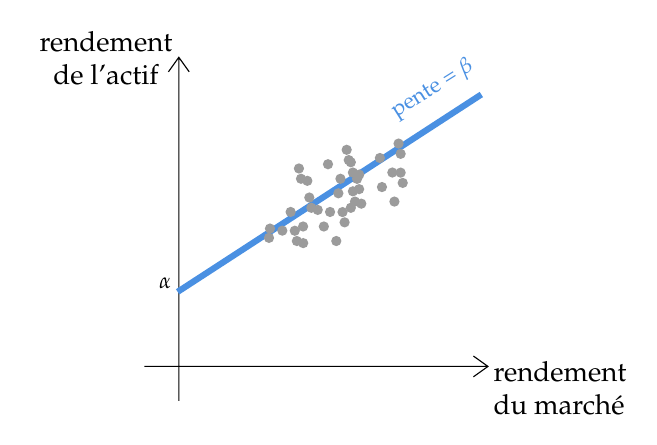
\begin{tikzpicture}[x=0.75pt,y=0.75pt,yscale=-1,xscale=1]
%uncomment if require: \path (0,208); %set diagram left start at 0, and has height of 208

%Shape: Axis 2D [id:dp954299495869529] 
\draw  (102,180.95) -- (267.5,180.95)(118.55,32) -- (118.55,197.5) (260.5,175.95) -- (267.5,180.95) -- (260.5,185.95) (113.55,39) -- (118.55,32) -- (123.55,39)  ;
%Straight Lines [id:da7226226944481302] 
\draw [color={rgb, 255:red, 74; green, 144; blue, 226 }  ,draw opacity=1 ][line width=2.25]    (264.3,49.92) -- (118,145) ;
%Shape: Circle [id:dp34497809539226076] 
\draw  [draw opacity=0][fill={rgb, 255:red, 155; green, 155; blue, 155 }  ,fill opacity=1 ] (159.52,119) .. controls (159.52,117.63) and (160.63,116.52) .. (162,116.52) .. controls (163.37,116.52) and (164.48,117.63) .. (164.48,119) .. controls (164.48,120.37) and (163.37,121.48) .. (162,121.48) .. controls (160.63,121.48) and (159.52,120.37) .. (159.52,119) -- cycle ;
%Shape: Circle [id:dp6402608510945291] 
\draw  [draw opacity=0][fill={rgb, 255:red, 155; green, 155; blue, 155 }  ,fill opacity=1 ] (165.95,115.52) .. controls (165.95,114.16) and (167.06,113.05) .. (168.43,113.05) .. controls (169.79,113.05) and (170.9,114.16) .. (170.9,115.52) .. controls (170.9,116.89) and (169.79,118) .. (168.43,118) .. controls (167.06,118) and (165.95,116.89) .. (165.95,115.52) -- cycle ;
%Shape: Circle [id:dp8456764702313726] 
\draw  [draw opacity=0][fill={rgb, 255:red, 155; green, 155; blue, 155 }  ,fill opacity=1 ] (160,114.52) .. controls (160,113.16) and (161.11,112.05) .. (162.48,112.05) .. controls (163.84,112.05) and (164.95,113.16) .. (164.95,114.52) .. controls (164.95,115.89) and (163.84,117) .. (162.48,117) .. controls (161.11,117) and (160,115.89) .. (160,114.52) -- cycle ;
%Shape: Circle [id:dp9296589117050036] 
\draw  [draw opacity=0][fill={rgb, 255:red, 155; green, 155; blue, 155 }  ,fill opacity=1 ] (175.95,113.52) .. controls (175.95,112.16) and (177.06,111.05) .. (178.43,111.05) .. controls (179.79,111.05) and (180.9,112.16) .. (180.9,113.52) .. controls (180.9,114.89) and (179.79,116) .. (178.43,116) .. controls (177.06,116) and (175.95,114.89) .. (175.95,113.52) -- cycle ;
%Shape: Circle [id:dp32028035526501264] 
\draw  [draw opacity=0][fill={rgb, 255:red, 155; green, 155; blue, 155 }  ,fill opacity=1 ] (169.95,106.52) .. controls (169.95,105.16) and (171.06,104.05) .. (172.43,104.05) .. controls (173.79,104.05) and (174.9,105.16) .. (174.9,106.52) .. controls (174.9,107.89) and (173.79,109) .. (172.43,109) .. controls (171.06,109) and (169.95,107.89) .. (169.95,106.52) -- cycle ;
%Shape: Circle [id:dp4483415592018749] 
\draw  [draw opacity=0][fill={rgb, 255:red, 155; green, 155; blue, 155 }  ,fill opacity=1 ] (179.95,104.52) .. controls (179.95,103.16) and (181.06,102.05) .. (182.43,102.05) .. controls (183.79,102.05) and (184.9,103.16) .. (184.9,104.52) .. controls (184.9,105.89) and (183.79,107) .. (182.43,107) .. controls (181.06,107) and (179.95,105.89) .. (179.95,104.52) -- cycle ;
%Shape: Circle [id:dp7294239015186668] 
\draw  [draw opacity=0][fill={rgb, 255:red, 155; green, 155; blue, 155 }  ,fill opacity=1 ] (178.95,99.57) .. controls (178.95,98.21) and (180.06,97.1) .. (181.43,97.1) .. controls (182.79,97.1) and (183.9,98.21) .. (183.9,99.57) .. controls (183.9,100.94) and (182.79,102.05) .. (181.43,102.05) .. controls (180.06,102.05) and (178.95,100.94) .. (178.95,99.57) -- cycle ;
%Shape: Circle [id:dp26318786151365026] 
\draw  [draw opacity=0][fill={rgb, 255:red, 155; green, 155; blue, 155 }  ,fill opacity=1 ] (188.95,106.52) .. controls (188.95,105.16) and (190.06,104.05) .. (191.43,104.05) .. controls (192.79,104.05) and (193.9,105.16) .. (193.9,106.52) .. controls (193.9,107.89) and (192.79,109) .. (191.43,109) .. controls (190.06,109) and (188.95,107.89) .. (188.95,106.52) -- cycle ;
%Shape: Circle [id:dp6296378002703897] 
\draw  [draw opacity=0][fill={rgb, 255:red, 155; green, 155; blue, 155 }  ,fill opacity=1 ] (183,105.52) .. controls (183,104.16) and (184.11,103.05) .. (185.48,103.05) .. controls (186.84,103.05) and (187.95,104.16) .. (187.95,105.52) .. controls (187.95,106.89) and (186.84,108) .. (185.48,108) .. controls (184.11,108) and (183,106.89) .. (183,105.52) -- cycle ;
%Shape: Circle [id:dp3909707695009883] 
\draw  [draw opacity=0][fill={rgb, 255:red, 155; green, 155; blue, 155 }  ,fill opacity=1 ] (198.95,104.52) .. controls (198.95,103.16) and (200.06,102.05) .. (201.43,102.05) .. controls (202.79,102.05) and (203.9,103.16) .. (203.9,104.52) .. controls (203.9,105.89) and (202.79,107) .. (201.43,107) .. controls (200.06,107) and (198.95,105.89) .. (198.95,104.52) -- cycle ;
%Shape: Circle [id:dp37192864439485507] 
\draw  [draw opacity=0][fill={rgb, 255:red, 155; green, 155; blue, 155 }  ,fill opacity=1 ] (192.95,97.52) .. controls (192.95,96.16) and (194.06,95.05) .. (195.43,95.05) .. controls (196.79,95.05) and (197.9,96.16) .. (197.9,97.52) .. controls (197.9,98.89) and (196.79,100) .. (195.43,100) .. controls (194.06,100) and (192.95,98.89) .. (192.95,97.52) -- cycle ;
%Shape: Circle [id:dp9063049345924845] 
\draw  [draw opacity=0][fill={rgb, 255:red, 155; green, 155; blue, 155 }  ,fill opacity=1 ] (202.95,95.52) .. controls (202.95,94.16) and (204.06,93.05) .. (205.43,93.05) .. controls (206.79,93.05) and (207.9,94.16) .. (207.9,95.52) .. controls (207.9,96.89) and (206.79,98) .. (205.43,98) .. controls (204.06,98) and (202.95,96.89) .. (202.95,95.52) -- cycle ;
%Shape: Circle [id:dp04049095390820612] 
\draw  [draw opacity=0][fill={rgb, 255:red, 155; green, 155; blue, 155 }  ,fill opacity=1 ] (201.95,90.57) .. controls (201.95,89.21) and (203.06,88.1) .. (204.43,88.1) .. controls (205.79,88.1) and (206.9,89.21) .. (206.9,90.57) .. controls (206.9,91.94) and (205.79,93.05) .. (204.43,93.05) .. controls (203.06,93.05) and (201.95,91.94) .. (201.95,90.57) -- cycle ;
%Shape: Circle [id:dp6059624038987319] 
\draw  [draw opacity=0][fill={rgb, 255:red, 155; green, 155; blue, 155 }  ,fill opacity=1 ] (172.95,120.52) .. controls (172.95,119.16) and (174.06,118.05) .. (175.43,118.05) .. controls (176.79,118.05) and (177.9,119.16) .. (177.9,120.52) .. controls (177.9,121.89) and (176.79,123) .. (175.43,123) .. controls (174.06,123) and (172.95,121.89) .. (172.95,120.52) -- cycle ;
%Shape: Circle [id:dp3269650983328478] 
\draw  [draw opacity=0][fill={rgb, 255:red, 155; green, 155; blue, 155 }  ,fill opacity=1 ] (171.95,115.57) .. controls (171.95,114.21) and (173.06,113.1) .. (174.43,113.1) .. controls (175.79,113.1) and (176.9,114.21) .. (176.9,115.57) .. controls (176.9,116.94) and (175.79,118.05) .. (174.43,118.05) .. controls (173.06,118.05) and (171.95,116.94) .. (171.95,115.57) -- cycle ;
%Shape: Circle [id:dp7344316786920082] 
\draw  [draw opacity=0][fill={rgb, 255:red, 155; green, 155; blue, 155 }  ,fill opacity=1 ] (176,121.52) .. controls (176,120.16) and (177.11,119.05) .. (178.48,119.05) .. controls (179.84,119.05) and (180.95,120.16) .. (180.95,121.52) .. controls (180.95,122.89) and (179.84,124) .. (178.48,124) .. controls (177.11,124) and (176,122.89) .. (176,121.52) -- cycle ;
%Shape: Circle [id:dp9043815174185361] 
\draw  [draw opacity=0][fill={rgb, 255:red, 155; green, 155; blue, 155 }  ,fill opacity=1 ] (191.95,120.52) .. controls (191.95,119.16) and (193.06,118.05) .. (194.43,118.05) .. controls (195.79,118.05) and (196.9,119.16) .. (196.9,120.52) .. controls (196.9,121.89) and (195.79,123) .. (194.43,123) .. controls (193.06,123) and (191.95,121.89) .. (191.95,120.52) -- cycle ;
%Shape: Circle [id:dp6403448546401829] 
\draw  [draw opacity=0][fill={rgb, 255:red, 155; green, 155; blue, 155 }  ,fill opacity=1 ] (185.95,113.52) .. controls (185.95,112.16) and (187.06,111.05) .. (188.43,111.05) .. controls (189.79,111.05) and (190.9,112.16) .. (190.9,113.52) .. controls (190.9,114.89) and (189.79,116) .. (188.43,116) .. controls (187.06,116) and (185.95,114.89) .. (185.95,113.52) -- cycle ;
%Shape: Circle [id:dp9756624389793735] 
\draw  [draw opacity=0][fill={rgb, 255:red, 155; green, 155; blue, 155 }  ,fill opacity=1 ] (195.95,111.52) .. controls (195.95,110.16) and (197.06,109.05) .. (198.43,109.05) .. controls (199.79,109.05) and (200.9,110.16) .. (200.9,111.52) .. controls (200.9,112.89) and (199.79,114) .. (198.43,114) .. controls (197.06,114) and (195.95,112.89) .. (195.95,111.52) -- cycle ;
%Shape: Circle [id:dp6881446735982482] 
\draw  [draw opacity=0][fill={rgb, 255:red, 155; green, 155; blue, 155 }  ,fill opacity=1 ] (194.95,106.57) .. controls (194.95,105.21) and (196.06,104.1) .. (197.43,104.1) .. controls (198.79,104.1) and (199.9,105.21) .. (199.9,106.57) .. controls (199.9,107.94) and (198.79,109.05) .. (197.43,109.05) .. controls (196.06,109.05) and (194.95,107.94) .. (194.95,106.57) -- cycle ;
%Shape: Circle [id:dp9019609351617717] 
\draw  [draw opacity=0][fill={rgb, 255:red, 155; green, 155; blue, 155 }  ,fill opacity=1 ] (174.95,90.52) .. controls (174.95,89.16) and (176.06,88.05) .. (177.43,88.05) .. controls (178.79,88.05) and (179.9,89.16) .. (179.9,90.52) .. controls (179.9,91.89) and (178.79,93) .. (177.43,93) .. controls (176.06,93) and (174.95,91.89) .. (174.95,90.52) -- cycle ;
%Shape: Circle [id:dp5095757141009629] 
\draw  [draw opacity=0][fill={rgb, 255:red, 155; green, 155; blue, 155 }  ,fill opacity=1 ] (173.95,85.57) .. controls (173.95,84.21) and (175.06,83.1) .. (176.43,83.1) .. controls (177.79,83.1) and (178.9,84.21) .. (178.9,85.57) .. controls (178.9,86.94) and (177.79,88.05) .. (176.43,88.05) .. controls (175.06,88.05) and (173.95,86.94) .. (173.95,85.57) -- cycle ;
%Shape: Circle [id:dp26502193850533184] 
\draw  [draw opacity=0][fill={rgb, 255:red, 155; green, 155; blue, 155 }  ,fill opacity=1 ] (178,91.52) .. controls (178,90.16) and (179.11,89.05) .. (180.48,89.05) .. controls (181.84,89.05) and (182.95,90.16) .. (182.95,91.52) .. controls (182.95,92.89) and (181.84,94) .. (180.48,94) .. controls (179.11,94) and (178,92.89) .. (178,91.52) -- cycle ;
%Shape: Circle [id:dp6985436023539344] 
\draw  [draw opacity=0][fill={rgb, 255:red, 155; green, 155; blue, 155 }  ,fill opacity=1 ] (193.95,90.52) .. controls (193.95,89.16) and (195.06,88.05) .. (196.43,88.05) .. controls (197.79,88.05) and (198.9,89.16) .. (198.9,90.52) .. controls (198.9,91.89) and (197.79,93) .. (196.43,93) .. controls (195.06,93) and (193.95,91.89) .. (193.95,90.52) -- cycle ;
%Shape: Circle [id:dp2949791823193908] 
\draw  [draw opacity=0][fill={rgb, 255:red, 155; green, 155; blue, 155 }  ,fill opacity=1 ] (187.95,83.52) .. controls (187.95,82.16) and (189.06,81.05) .. (190.43,81.05) .. controls (191.79,81.05) and (192.9,82.16) .. (192.9,83.52) .. controls (192.9,84.89) and (191.79,86) .. (190.43,86) .. controls (189.06,86) and (187.95,84.89) .. (187.95,83.52) -- cycle ;
%Shape: Circle [id:dp22083446469496448] 
\draw  [draw opacity=0][fill={rgb, 255:red, 155; green, 155; blue, 155 }  ,fill opacity=1 ] (197.95,81.52) .. controls (197.95,80.16) and (199.06,79.05) .. (200.43,79.05) .. controls (201.79,79.05) and (202.9,80.16) .. (202.9,81.52) .. controls (202.9,82.89) and (201.79,84) .. (200.43,84) .. controls (199.06,84) and (197.95,82.89) .. (197.95,81.52) -- cycle ;
%Shape: Circle [id:dp2371069564113233] 
\draw  [draw opacity=0][fill={rgb, 255:red, 155; green, 155; blue, 155 }  ,fill opacity=1 ] (196.95,76.57) .. controls (196.95,75.21) and (198.06,74.1) .. (199.43,74.1) .. controls (200.79,74.1) and (201.9,75.21) .. (201.9,76.57) .. controls (201.9,77.94) and (200.79,79.05) .. (199.43,79.05) .. controls (198.06,79.05) and (196.95,77.94) .. (196.95,76.57) -- cycle ;
%Shape: Circle [id:dp9867728920735555] 
\draw  [draw opacity=0][fill={rgb, 255:red, 155; green, 155; blue, 155 }  ,fill opacity=1 ] (200.95,101.52) .. controls (200.95,100.16) and (202.06,99.05) .. (203.43,99.05) .. controls (204.79,99.05) and (205.9,100.16) .. (205.9,101.52) .. controls (205.9,102.89) and (204.79,104) .. (203.43,104) .. controls (202.06,104) and (200.95,102.89) .. (200.95,101.52) -- cycle ;
%Shape: Circle [id:dp8285540753909157] 
\draw  [draw opacity=0][fill={rgb, 255:red, 155; green, 155; blue, 155 }  ,fill opacity=1 ] (199.95,96.57) .. controls (199.95,95.21) and (201.06,94.1) .. (202.43,94.1) .. controls (203.79,94.1) and (204.9,95.21) .. (204.9,96.57) .. controls (204.9,97.94) and (203.79,99.05) .. (202.43,99.05) .. controls (201.06,99.05) and (199.95,97.94) .. (199.95,96.57) -- cycle ;
%Shape: Circle [id:dp5866262608543329] 
\draw  [draw opacity=0][fill={rgb, 255:red, 155; green, 155; blue, 155 }  ,fill opacity=1 ] (204,102.52) .. controls (204,101.16) and (205.11,100.05) .. (206.48,100.05) .. controls (207.84,100.05) and (208.95,101.16) .. (208.95,102.52) .. controls (208.95,103.89) and (207.84,105) .. (206.48,105) .. controls (205.11,105) and (204,103.89) .. (204,102.52) -- cycle ;
%Shape: Circle [id:dp4508862725275873] 
\draw  [draw opacity=0][fill={rgb, 255:red, 155; green, 155; blue, 155 }  ,fill opacity=1 ] (219.95,101.52) .. controls (219.95,100.16) and (221.06,99.05) .. (222.43,99.05) .. controls (223.79,99.05) and (224.9,100.16) .. (224.9,101.52) .. controls (224.9,102.89) and (223.79,104) .. (222.43,104) .. controls (221.06,104) and (219.95,102.89) .. (219.95,101.52) -- cycle ;
%Shape: Circle [id:dp730533643750001] 
\draw  [draw opacity=0][fill={rgb, 255:red, 155; green, 155; blue, 155 }  ,fill opacity=1 ] (213.95,94.52) .. controls (213.95,93.16) and (215.06,92.05) .. (216.43,92.05) .. controls (217.79,92.05) and (218.9,93.16) .. (218.9,94.52) .. controls (218.9,95.89) and (217.79,97) .. (216.43,97) .. controls (215.06,97) and (213.95,95.89) .. (213.95,94.52) -- cycle ;
%Shape: Circle [id:dp9360442346841504] 
\draw  [draw opacity=0][fill={rgb, 255:red, 155; green, 155; blue, 155 }  ,fill opacity=1 ] (223.95,92.52) .. controls (223.95,91.16) and (225.06,90.05) .. (226.43,90.05) .. controls (227.79,90.05) and (228.9,91.16) .. (228.9,92.52) .. controls (228.9,93.89) and (227.79,95) .. (226.43,95) .. controls (225.06,95) and (223.95,93.89) .. (223.95,92.52) -- cycle ;
%Shape: Circle [id:dp025076547083871636] 
\draw  [draw opacity=0][fill={rgb, 255:red, 155; green, 155; blue, 155 }  ,fill opacity=1 ] (222.95,87.57) .. controls (222.95,86.21) and (224.06,85.1) .. (225.43,85.1) .. controls (226.79,85.1) and (227.9,86.21) .. (227.9,87.57) .. controls (227.9,88.94) and (226.79,90.05) .. (225.43,90.05) .. controls (224.06,90.05) and (222.95,88.94) .. (222.95,87.57) -- cycle ;
%Shape: Circle [id:dp5181244456176788] 
\draw  [draw opacity=0][fill={rgb, 255:red, 155; green, 155; blue, 155 }  ,fill opacity=1 ] (199.95,87.52) .. controls (199.95,86.16) and (201.06,85.05) .. (202.43,85.05) .. controls (203.79,85.05) and (204.9,86.16) .. (204.9,87.52) .. controls (204.9,88.89) and (203.79,90) .. (202.43,90) .. controls (201.06,90) and (199.95,88.89) .. (199.95,87.52) -- cycle ;
%Shape: Circle [id:dp196680423509215] 
\draw  [draw opacity=0][fill={rgb, 255:red, 155; green, 155; blue, 155 }  ,fill opacity=1 ] (198.95,82.57) .. controls (198.95,81.21) and (200.06,80.1) .. (201.43,80.1) .. controls (202.79,80.1) and (203.9,81.21) .. (203.9,82.57) .. controls (203.9,83.94) and (202.79,85.05) .. (201.43,85.05) .. controls (200.06,85.05) and (198.95,83.94) .. (198.95,82.57) -- cycle ;
%Shape: Circle [id:dp2954672562656153] 
\draw  [draw opacity=0][fill={rgb, 255:red, 155; green, 155; blue, 155 }  ,fill opacity=1 ] (203,88.52) .. controls (203,87.16) and (204.11,86.05) .. (205.48,86.05) .. controls (206.84,86.05) and (207.95,87.16) .. (207.95,88.52) .. controls (207.95,89.89) and (206.84,91) .. (205.48,91) .. controls (204.11,91) and (203,89.89) .. (203,88.52) -- cycle ;
%Shape: Circle [id:dp8548165127565825] 
\draw  [draw opacity=0][fill={rgb, 255:red, 155; green, 155; blue, 155 }  ,fill opacity=1 ] (218.95,87.52) .. controls (218.95,86.16) and (220.06,85.05) .. (221.43,85.05) .. controls (222.79,85.05) and (223.9,86.16) .. (223.9,87.52) .. controls (223.9,88.89) and (222.79,90) .. (221.43,90) .. controls (220.06,90) and (218.95,88.89) .. (218.95,87.52) -- cycle ;
%Shape: Circle [id:dp05963106369983273] 
\draw  [draw opacity=0][fill={rgb, 255:red, 155; green, 155; blue, 155 }  ,fill opacity=1 ] (212.95,80.52) .. controls (212.95,79.16) and (214.06,78.05) .. (215.43,78.05) .. controls (216.79,78.05) and (217.9,79.16) .. (217.9,80.52) .. controls (217.9,81.89) and (216.79,83) .. (215.43,83) .. controls (214.06,83) and (212.95,81.89) .. (212.95,80.52) -- cycle ;
%Shape: Circle [id:dp22231923672229503] 
\draw  [draw opacity=0][fill={rgb, 255:red, 155; green, 155; blue, 155 }  ,fill opacity=1 ] (222.95,78.52) .. controls (222.95,77.16) and (224.06,76.05) .. (225.43,76.05) .. controls (226.79,76.05) and (227.9,77.16) .. (227.9,78.52) .. controls (227.9,79.89) and (226.79,81) .. (225.43,81) .. controls (224.06,81) and (222.95,79.89) .. (222.95,78.52) -- cycle ;
%Shape: Circle [id:dp6996544025433038] 
\draw  [draw opacity=0][fill={rgb, 255:red, 155; green, 155; blue, 155 }  ,fill opacity=1 ] (221.95,73.57) .. controls (221.95,72.21) and (223.06,71.1) .. (224.43,71.1) .. controls (225.79,71.1) and (226.9,72.21) .. (226.9,73.57) .. controls (226.9,74.94) and (225.79,76.05) .. (224.43,76.05) .. controls (223.06,76.05) and (221.95,74.94) .. (221.95,73.57) -- cycle ;

% Text Node
\draw (269,177) node [anchor=north west][inner sep=0.75pt]   [align=left] {rendement \\du marché};
% Text Node
\draw (46,18) node [anchor=north west][inner sep=0.75pt]   [align=left] {\begin{minipage}[lt]{54.3235pt}\setlength\topsep{0pt}
\begin{center}
rendement \\de l'actif
\end{center}

\end{minipage}};
% Text Node
\draw (105,137) node [anchor=north west][inner sep=0.75pt]  [font=\footnotesize] [align=left] {\begin{minipage}[lt]{8.67pt}\setlength\topsep{0pt}
\begin{center}
$\displaystyle \alpha $
\end{center}

\end{minipage}};
% Text Node
\draw (217.54,54.42) node [anchor=north west][inner sep=0.75pt]  [color={rgb, 255:red, 74; green, 144; blue, 226 }  ,opacity=1 ,rotate=-327.82] [align=left] {{\footnotesize pente = $\displaystyle \beta $}};


\end{tikzpicture}
\end{center}

\begin{definitionNOHFILL}[Le modèle d'évaluation des actifs financiers (MÉDAF)]
Le MÉDAF nous permet de trouver le coût du capital $r_{i}$ (alias, le rendement espéré $\text{E}[R_{i}]$) d'un actif en posant que le niveau de risque systématique de base correspond au niveau de risque du portefeuille du marché. \\

L'équation du MÉDAF est \lfbox[formula]{$r_{i}	=	\text{E}[R_{i}]	=	r_{f} + \beta_{i}(\text{E}[R_{M}]	-	r_{f})$}.

\begin{itemize}
	\item	En anglais, \og \textit{Capital Asset Pricing Model (CAPM)} \fg{} ;
	\item	En régression, ceci correspond à l'équation pour la prévision $\hat{y}_{i}	=	\hat{\beta}_{0} + \hat{\beta}_{1}x_{i}$ ;
	\item	Alors, le vrai rendement de l'investissement $i$ est $r_{f} + \beta_{i}(r_{M} -  r_{f}) \textcolor{teal}{+ \alpha_{i}}$.
\end{itemize}
\end{definitionNOHFILL}

\begin{conceptgen}{Hypothèses du MÉDAF}
\begin{enumerate}
	\item	Les investisseurs sont des preneurs de prix.
		\begin{itemize}
		\item	C'est à dire qu'ils transiger les titres aux prix compétitifs du marché sans pouvoir les influencer (concept de macro.) ;
		\item	Il n'y a pas de taxes ni de frais de transactions ;
		\item	Les investisseurs peuvent emprunter et prêter de l'argent au taux sans risque.
		\end{itemize}
	\item	Les investisseurs détiennent uniquement des portefeuilles efficients.
		\begin{itemize}
		\item	Ceci implique que les investisseurs sont rationnels, qu’ils ont une aversion au risque et qu'ils cherchent à maximiser leurs investissements.
		\item	C'est à dire que pour un niveau de risque (volatilité) donné, il n'y a pas de portefeuilles avec un rendement supérieur. 
		\end{itemize}
	\item	Les investisseurs ont des attentes homogènes pour les volatilités, les corrélations et les rendements espérés de titres financiers.
		\begin{itemize}
		\item	Des chercheurs ont trouvé que si les investisseurs n'ont pas des attentes \textit{homogènes}, le MÉDAF n'est pas nécessairement invalide tant qu'ils ont des attentes \textit{\textbf{rationnelles}}.
		\end{itemize}
\end{enumerate}
\end{conceptgen}

\begin{definitionNOHFILLsub}[Droite du marché des titres]
Représentation graphique du MÉDAF.

\begin{center}
\tikzset{every picture/.style={line width=0.75pt}} %set default line width to 0.75pt        

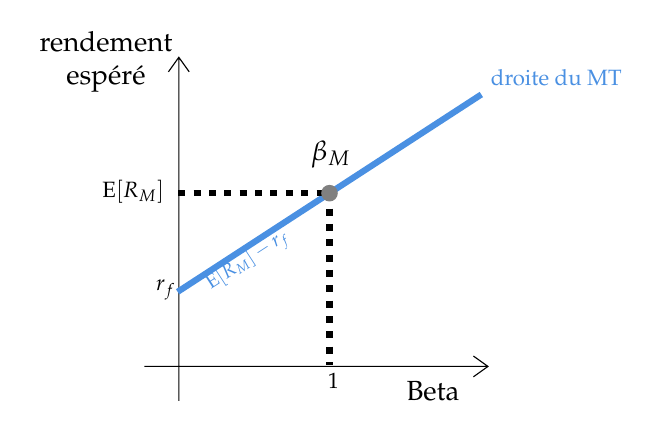
\begin{tikzpicture}[x=0.75pt,y=0.75pt,yscale=-1,xscale=1]
%uncomment if require: \path (0,208); %set diagram left start at 0, and has height of 208

%Shape: Axis 2D [id:dp954299495869529] 
\draw  (102,180.95) -- (267.5,180.95)(118.55,32) -- (118.55,197.5) (260.5,175.95) -- (267.5,180.95) -- (260.5,185.95) (113.55,39) -- (118.55,32) -- (123.55,39)  ;
%Straight Lines [id:da7226226944481302] 
\draw [color={rgb, 255:red, 74; green, 144; blue, 226 }  ,draw opacity=1 ][line width=2.25]    (264.3,49.92) -- (118,145) ;
%Straight Lines [id:da8365355669623116] 
\draw [color={rgb, 255:red, 0; green, 0; blue, 0 }  ,draw opacity=1 ][line width=2.25]  [dash pattern={on 2.53pt off 3.02pt}]  (191.15,97.46) -- (191.15,180.32) ;
%Straight Lines [id:da7387452691634961] 
\draw [color={rgb, 255:red, 0; green, 0; blue, 0 }  ,draw opacity=1 ][line width=2.25]  [dash pattern={on 2.53pt off 3.02pt}]  (118.3,97.46) -- (191.15,97.46) ;
%Shape: Circle [id:dp5467744572484954] 
\draw  [draw opacity=0][fill={rgb, 255:red, 128; green, 128; blue, 128 }  ,fill opacity=1 ] (187.15,97.46) .. controls (187.15,95.25) and (188.94,93.46) .. (191.15,93.46) .. controls (193.36,93.46) and (195.15,95.25) .. (195.15,97.46) .. controls (195.15,99.67) and (193.36,101.46) .. (191.15,101.46) .. controls (188.94,101.46) and (187.15,99.67) .. (187.15,97.46) -- cycle ;

% Text Node
\draw (227,187) node [anchor=north west][inner sep=0.75pt]   [align=left] {Beta};
% Text Node
\draw (46,18) node [anchor=north west][inner sep=0.75pt]   [align=left] {\begin{minipage}[lt]{54.3235pt}\setlength\topsep{0pt}
\begin{center}
rendement \\espéré
\end{center}

\end{minipage}};
% Text Node
\draw (77,90) node [anchor=north west][inner sep=0.75pt]  [font=\footnotesize] [align=left] {\begin{minipage}[lt]{27.480500000000003pt}\setlength\topsep{0pt}
\begin{center}
$\displaystyle \text{E}[ R_{M}]$
\end{center}

\end{minipage}};
% Text Node
\draw (267.69,36.47) node [anchor=north west][inner sep=0.75pt]  [color={rgb, 255:red, 74; green, 144; blue, 226 }  ,opacity=1 ] [align=left] {{\footnotesize droite du MT}};
% Text Node
\draw (186,183) node [anchor=north west][inner sep=0.75pt]  [font=\footnotesize] [align=left] {\begin{minipage}[lt]{8.67pt}\setlength\topsep{0pt}
\begin{center}
$\displaystyle 1$
\end{center}

\end{minipage}};
% Text Node
\draw (179,71) node [anchor=north west][inner sep=0.75pt]  [font=\normalsize] [align=left] {\begin{minipage}[lt]{17.3825pt}\setlength\topsep{0pt}
\begin{center}
$\displaystyle \beta _{M}$
\end{center}

\end{minipage}};
% Text Node
\draw (104,138) node [anchor=north west][inner sep=0.75pt]  [font=\footnotesize] [align=left] {\begin{minipage}[lt]{10.701500000000001pt}\setlength\topsep{0pt}
\begin{center}
$\displaystyle r_{f}$
\end{center}

\end{minipage}};
% Text Node
\draw (128.31,137.43) node [anchor=north west][inner sep=0.75pt]  [color={rgb, 255:red, 74; green, 144; blue, 226 }  ,opacity=1 ,rotate=-327] [align=left] {{\scriptsize $\displaystyle \text{E}[ R_{M}] -r_{f}$}};


\end{tikzpicture}
\end{center}

\begin{itemize}
	\item	En anglais, \og \textit{security market line (SML)} \fg{}.
\end{itemize}

\end{definitionNOHFILLsub}

\begin{rappel_enhanced}[Distinction entre la droite du MC et la droite du MT]
L'abscisse de la droite du marché des capitaux (MC) utilise la volatilité (alias le \textbf{risque total}).
\begin{itemize}
	\item	Seulement les portefeuilles efficients composés d'une combinaison de l'actif sans risque et du portefeuille du marché seront tracés.
\end{itemize}

L'abscisse de la droite du marché des titres (MT) utilise le beta (alias le \textbf{risque systémique}).
\begin{itemize}
	\item	Le \underline{risque non systémique est sans importance au MÉDAF} ;
	\item	Alors, la relation sous-jacente à la droite du MT ne se limite pas aux portefeuilles efficients.
\end{itemize}
\end{rappel_enhanced}


%\columnbreak
\subsubsection{Prime de risque du marché}
\begin{definitionNOHFILLsub}[Prime de risque du marché]
la prime de risque du marché correspond à l'écart entre le rendement espéré du marché et le taux sans risque : \lfbox[formula]{$\text{E}[R_{M}]	-	r_{f}$}.

Elle peut être approximée de deux façons :
\begin{enumerate}
	\item	La prime de risque historique.
	\item	L'approche fondamentale.
\end{enumerate}

\begin{itemize}
	\item	En anglais, \og \textit{Market Risk Premium} \fg{}.
\end{itemize}
\end{definitionNOHFILLsub}


\begin{definitionNOHFILLprop}[Prime de risque historique]
La prime de risque est calculé comme étant la moyenne historique de l'excédant du rendement du marché sur le taux sans risque.\\

\textbf{Limitations :}
\begin{itemize}
	\item	L'erreur type des prévisions est large.
	\item	Le passé n'est pas nécessairement garant de l'avenir.
\end{itemize}
\end{definitionNOHFILLprop}

\begin{definitionNOHFILLprop}[Approche fondamentale]
\begin{distributions}[Notation]
\begin{description}
	\item[$Div_{1}$]	Dividende payable au temps 1.
	\item[$P_{0}$]	Prix courant de l'action.
		\begin{itemize}
		\item	Le ratio $\frac{Div_{1}}{P_{0}}$ est le \textbf{rendement de l'action} (\og \textit{dividend yield} \fg{}).
		\end{itemize}
	\item[$g$]	Taux de croissance fixe des dividendes.
\end{description}
\end{distributions}

On pose un taux de croissance fixe des dividendes $g$ avec \lfbox[conditions]{$P_{0}	=	\frac{Div_{1}}{\text{E}[R_{M}]	-	g}$}. En réécrivant l'équation, on trouve que \lfbox[formula]{$\text{E}[R_{M}]	=	\frac{Div_{1}}{P_{0}} + g$}.\\

\textbf{Limitation :}
\begin{itemize}
%%%	------------------------
%%%	NOTES
%%%	+	clarifier l'écriture de cette phrase
%%%	------------------------
	\item	L'approche est adéquate seulement pour l'ensemble de marchés et non pour des actions individuelles.
\end{itemize}
\end{definitionNOHFILLprop}



\columnbreak
\subsubsection{Coût des capitaux d'emprunt}
Lorsque l'on cherche à estimer le coût de capitaux d'emprunt au lieu du coût de capitaux propres, il y a 2 méthodes : 
\begin{enumerate}
	\item	Ajustement du rendement de la dette.
	\item	MÉDAF avec les betas de dette.
\end{enumerate}

\begin{distributions}[Notation]
\begin{description}
	\item[$r_{d}$]	Coût des capitaux d'emprunt.
		\begin{itemize}
		\item	\og \textit{Debt cost of capital} \fg{}.
		\end{itemize}
	\item[$\beta_{d}$]	Beta de la dette.
\end{description}

Soit une obligation zéro-coupon avec :
\begin{description}
	\item[$y$]	Taux de rendement à l'échéance de l'obligation.
		\begin{itemize}
		\item	En anglais, \og \textit{yield to maturity (YTM) of the bond} \fg{}.
		\end{itemize}
	\item[$p$]	Probabilité de défaut de l'obligation.
	\item[$L$]	Espérance du montant de perte, par dollar de dette, s'il y a défaut
		\begin{itemize}
		\item	On représente $L$ par dollar de dette afin de l'inclure comme pourcentage dans l'équation de $r_{d}$ plus bas.
		\end{itemize}
\end{description}
\end{distributions}


\begin{definitionNOHFILLsub}[Ajustement du rendement de la dette]
Pour un investissement de 1\$ dans une obligation zéro-coupon
\begin{itemize}
	\item	sans risque de défaut, on obtient $(1 + y)\$$ dans un an.
	\item	avec risque de défaut, on obtient :
		\begin{itemize}
		\item	$(1 + y - L)\$$ dans un an avec probabilité $p$
		\item	$(1 + y)\$$ dans un an avec probabilité $(1 - p)$
		\end{itemize}
\end{itemize}

Donc, on trouve avec une moyenne pondérée des rendements \lfbox[formula]{$r_{d}	=	y	-	pL$}.
\end{definitionNOHFILLsub}

\begin{definitionNOHFILLprop}[MÉDAF avec les betas de dette]
Avec le MÉDAF, on réécrit \lfbox[formula]{$r_{d}	=	r_{f} + \beta_{d}\left(\shortstack{prime de risque\\ du marché}\right)$}.\\
\end{definitionNOHFILLprop}


\columnbreak
\subsubsection{Rendement requis pour un projet pleinement financé par des actions}
\label{sec:wacc_def}
On peut généraliser le MÉDAF afin d'estimer le rendement nécessaire pour un projet en remplaçant le beta de l'investissement par le beta du projet.

\begin{itemize}
	\item	Typiquement, on ne peut pas estimer le beta d'un projet directement puisque le projet n'est pas coté en bourse ;
	\item	En lieu, on utilise le beta \textit{d'entreprises semblables} ;
		\begin{itemize}
		\item	C'est à dire, des entreprises dont le secteur d'opération ou le risque est semblable à celui du projet.
		\end{itemize}
\end{itemize}

Si on compare le projet à une entreprise :
\begin{itemize}
	\item	Sans effet de levier, on applique l'équation du MÉDAF directement.
	\item	Avec effet de levier, on doit calculer le \textbf{coût du capital sans effet de levier}.
\end{itemize}

\begin{definitionNOHFILLsub}[Coût du capital et beta sans effet de levier]
\begin{distributions}[Notation]
\begin{description}
	\item[$r_{U}$]	Coût des capitaux propres sans effet de levier.
	\item[$\beta_{U}$]	Beta sans effet de levier.
	\item[$E$]	Valeur au marché de l'équité de l'entreprise.
	\item[$D$]	Valeur au marché de la dette de l'entreprise.
		\begin{itemize}
		\item	S'il y a des capitaux propres, on calcule $D - CP$.
		\end{itemize}
	\item[$r_{E}$]	Coût des capitaux propres avec levier.
	\item[$r_{D}$]	Coût des capitaux d'emprunt.
	\item[$w_{E}$]	Proportion de l'entreprise financée par des capitaux propres.
		\begin{itemize}
		\item	\lfbox[formula]{$w_{E}	=	\frac{E}{E + D}$}.
		\end{itemize}
	\item[$w_{D}$]	Proportion de l'entreprise financée par de la dette.
		\begin{itemize}
		\item	\lfbox[formula]{$w_{D}	=	\frac{D}{E + D}$}.
		\end{itemize}
\end{description}
\end{distributions}

Donc, on trouve : 
\begin{itemize}
	\item	le coût des capitaux propres sans effet de levier \lfbox[formula]{$r_{U}	=	w_{E} \cdot r_{E} + w_{D} \cdot r_{D}$}, et 
	\item	le beta sans effet de levier \lfbox[formula]{$\beta_{U}	=	w_{E} \cdot \beta_{E} + w_{D} \cdot \beta_{D}$} ;
	\item	En anglais, \og \textit{unlevered cost of capital} \fg{}.
\end{itemize}
\end{definitionNOHFILLsub}

\begin{definitionNOHFILLprop}[MÉDAF d'un projet pour une comparaison à une entreprise avec effet de levier]
Avec le MÉDAF, on réécrit \lfbox[formula]{$r_{U}	=	r_{f} + \beta_{U}\left(\shortstack{prime de risque\\ du marché}\right)$}.\\
\end{definitionNOHFILLprop}

\paragraph{Note}	La valeur d'une entreprise correspond à sa dette nette = $\text{dette}	-	\text{investissements à CT et l'encaisse}$ ; c'est à dire, $D - CP$.

%\columnbreak
\subsubsection{Rendement requis pour un projet avec effet de levier}
\begin{distributions}[Notation]
\begin{description}
	\item[$\tau_{C}$]	Taux d'imposition sur la dette.
\end{description}
\end{distributions}

Dans le cas où le projet doit être financé par des capitaux propre \textbf{\textit{et}} de la dette, on trouve le coût moyen pondéré du capital (CMPC) \lfbox[formula]{$r_{\text{CMPC}}	=	w_{E} r_{E} + w_{D} r_{D}(1 - \tau_{C})$}.
\begin{itemize}
	\item	Souvent, l'intérêt payable sur la dette est déductible d'impôts et donc on veut le coût de la dette après imposition ;
	\item	En anglais, \og \textit{weighted-average cost of capital (WACC)} \fg{}.
\end{itemize}

Le CMPC se base sur le coût des capitaux d'emprunt après imposition alors que le coût des capitaux propres sans effet de levier se base sur le coût des capitaux d'emprunt avant imposition. En bref :

\begin{center}
\begin{tabular}{| >{\columncolor{beaublue}}m{6cm} | >{\columncolor{beaublue}}m{6cm}  |}
\hline\rowcolor{airforceblue} 
\textcolor{white}{\textbf{Coût des capitaux propres sans effet de levier}}	&	\textcolor{white}{\textbf{CMPC}}		\\\specialrule{0.1em}{0em}{0em} 
Utilisé pour évaluer un projet financé sans emprunt ayant le même risque que l'entreprise	&	Utilisé pour évaluer un projet ayant le même financement et le même risque que l'entreprise	\\\hline
\end{tabular}
\end{center}


\columnbreak
\subsection{Modèles multi-factoriels}
\begin{rappel_enhanced}[Contexte]
Le MÉDAF pose que la volatilité des rendements du marché sont expliqué par \textbf{\textit{un seul facteur}}---le rendement sur le portefeuille du marché.\\
Le MÉDAF multi-factoriel prend plusieurs facteurs en considération pour estimer le rendement espéré. Ce modèle muti-factoriel est aussi connu comme la théorie de l'arbitrage de prix (\og \textit{arbitrage pricing theory (APT)} \fg{}).
\end{rappel_enhanced}
\begin{distributions}[Notation]
\begin{description}
	\item[$N$]	Nombre de facteurs.
	\item[$\beta_{{\color{teal}i}}^{{\color{burntorange}F}{\color{amethyst}n}}$]	Beta de l'actif ${\color{teal}i}$ au {\color{burntorange}facteur} ${\color{amethyst}n}$ en tenant les autres facteurs constants.
\end{description}
\end{distributions}
On trouve que l'équation de l'APT est \lfbox[formula]{$\text{E}[R_{i}]	=	r_{f} + \sum_{n = 1}^{N} \beta_{i}^{Fn}\left(\text{E}[R_{Fn}]	-	r_{f}\right)$}.

L'APT est semblable au CAPM mais comporte des hypothèses moins restrictives :
\begin{conceptgen}{Hypothèses de l'APT}
\begin{enumerate}
	\item	Un modèle multi-factoriel décrit les rendements d'un actif sans toutefois indiquer le nombre de facteurs.
	\item	Le risque non systémique peut être éliminé avec de la diversification et n'est pas tarifé.
	\item	Il n'y a pas d'arbitrage.
\end{enumerate}
\end{conceptgen}

\begin{definitionNOHFILLprop}[Portefeuilles multi-factoriels autofinançants]
Si les tous les portefeuilles multi-factoriels sont autofinançant, on peut récrire : \lfbox[formula]{$\text{E}[R_{i}]	=	r_{f} + \sum_{n = 1}^{N} \beta_{i}^{Fn}\text{E}[R_{Fn}]$}.
\begin{itemize}
	\item	Les $\beta$s vont sommer à 0 au lieu de 1.
\end{itemize}
\end{definitionNOHFILLprop}


\subsubsection{Fama-French-Carhart (FFC)}
\begin{definitionNOHFILL}[Notation]
La spécification de facteurs FFC est la plus courante avec le \textbf{marché}, la \textbf{capitalisation boursière}, le \textbf{ratio cours / valeur comptable} et \textbf{l'élan} comme facteurs.
\begin{itemize}
	\item	L'idée de la stratégie avec la spécification de FFC est de tirer profit du fait que ces portefeuilles semblent avoir des $\alpha$ positifs.
\end{itemize}

\begin{description}
	\item[$M$]	Portefeuille du marché.
		\begin{itemize}
		\item	Prend en considération le risque des capitaux propres.
		\end{itemize}
	\item[$GMP$]	Portefeuille gros-moins-petit.
		\begin{itemize}
		\item	En anglais, \og \textit{small-minus-big (SMB)} \fg{} ;
		\item	Prends en considération la diversité de la taille des entreprises selon la capitalisation boursière ;
		\item	On l'estime comme la différence entre le rendement d'entreprises avec une capitalisation boursière élevée et faible $\text{E}[R_{GMP}]	=	\text{E}[R_{G}]	-	\text{E}[R_{P}]$.
		\end{itemize}
	\item[$EMF$]	Portefeuille élevé moins faible.
		\begin{itemize}
		\item	En anglais, \og \textit{high-minus-low (HML)} \fg{} ;
		\item	Prends en considération la diversité des rendements sur des actions de valeur et des actions de croissance ;
		\item	Les action de valeur sont définies comme des actions avec un ratio cours-valeur comptable élevé alors que des actions de croissance ont un ratio cours-valeurs comptable faible ;
		\item	On l'estime comme la différence entre le rendement d'entreprises avec un ratio élevé et faible $\text{E}[R_{EMF}]	=	\text{E}[R_{E}]	-	\text{E}[R_{F}]$.
		\end{itemize}
	\item[$AVE$]	Portefeuille de l'année avant l'élan d'une entreprise.
		\begin{itemize}
		\item	En anglais, \og \textit{prior 1-year momentum (PR1YR)} \fg{} ;
		\item	Prends en considération l'élan d'une compagnie ;
		\item	On l'estime comme la différence entre le rendements des gagnants et des perdants de l'année passée $\text{E}[R_{AVE}]	=	\text{E}[R_{GAVE}]	-	\text{E}[R_{PAVE}]$..
		\end{itemize}
\end{description}

On trouve que \lfbox[formula]{$\text{E}[R_{i}]	=	r_{f} + \beta_{i}^{M}\left(\text{E}[R_{M}] - r_{f}\right) + \beta_{i}^{GMP} \text{E}[R_{GMP}]$}	\lfbox[formula]{$+ \beta_{i}^{EMF} \text{E}[R_{EMF}]	 + \beta_{i}^{AVE} \text{E}[R_{AVE}]$}.
\end{definitionNOHFILL}



\newpage
\setcounter{section}{38} % dut sauter 9 à cause d'un problème avec le toc
\section{Market Efficiency and Behavioural Finance}
\begin{definitionNOHFILL}[Marché efficient]
Marché dont les prix des titres financiers s'ajustent rapidement à toutes nouvelles informations ; les prix reflètent toute l'information disponible.


%%%	------------------------
%%%	NOTES
%%%	+	Mieux expliquer ça.
%%%	------------------------
Si un marché :
\begin{description}
	\item[est efficient]	le prix de l'action reflètent toute l'information disponible.
		\begin{itemize}
		\item	Les stratégies passives sont optimales.
		\end{itemize}
	\item[n'est pas efficient]	le prix de l'action peut ne pas être représentatif de sa vraie valeur.
		\begin{itemize}
		\item	Des stratégies actives peuvent être supérieures à une stratégie passive.
		\end{itemize}
\end{description}

\begin{itemize}
	\item	En anglais, \og \textit{efficient market hypothesis (EMH)} \fg{}.
\end{itemize}
\end{definitionNOHFILL}


\subsection{Formes d'efficience de marché (EM)}
En bref : 
\begin{center}
\begin{tabular}{| >{\columncolor{beaublue}}c | >{\columncolor{beaublue}}m{2cm}<{\centering}   | >{\columncolor{beaublue}}m{2cm}<{\centering}  | >{\columncolor{beaublue}}m{2cm}<{\centering}  |}
\hline\rowcolor{airforceblue} 
\textcolor{white}{\textbf{Forme d'EM}}	&	\textcolor{white}{\textbf{Données historiques}}	&	\textcolor{white}{\textbf{Informatique publique}}	&	\textcolor{white}{\textbf{Information privée}}		\\\hline
\og \textit{Weak} \fg{} 	&	$\checkmark$	&		&		\\\hline
\og \textit{Semi-strong} \fg{} 	&	$\checkmark$	&	$\checkmark$	&		\\\hline
\og \textit{Strong} \fg{} 	&	$\checkmark$	&	$\checkmark$	&	$\checkmark$	\\\hline
\end{tabular}
\end{center}


\begin{definitionNOHFILLsub}[Hypothèse d'EM \og \textit{weak form} \fg{}]
Pose que les prix de titres financiers reflètent \textbf{toute l'information historique du marché}. 

\begin{itemize}
	\item	Cette théorie pose donc que le prix d'un titre prend déjà en compte ses rendements, ou tendances de rendements, antérieurs et donc que ses rendements \textit{futurs} sont indépendants du passé.
	\item	Cette théorie implique que l'on ne peut pas obtenir des rendements supérieurs \underline{\textbf{de façon régulière}} en analysant les rendements historiques.
\end{itemize}
\end{definitionNOHFILLsub}


\begin{definitionNOHFILLsub}[Hypothèse d'EM \og \textit{semi-strong form} \fg{}]
Pose que les prix de titres financiers reflètent \textbf{toute l'information disponible publiquement}, y compris les données historiques du marché.

\begin{itemize}
	\item	Cette théorie pose que les prix de titres financiers s'ajustent au moment que de nouvelles informations sont rendues disponibles.
		\begin{itemize}
		\item	P. ex. : diffusion publique de gains inférieurs aux attentes ou une mise à pied où le prix de l'action décroît.
		\item	P. ex., l'annonce d'une fusion où le prix de l'action augmente puisqu'elles seront rachetées à un prix supérieur à celui du marché.
		\end{itemize}
	\item	Cette théorie implique que l'on ne peut pas obtenir des rendements supérieurs \underline{\textbf{de façon régulière}} en analysant des rapports annuels puisque l'information est déjà prises en considération dans le prix du titre.
\end{itemize}
\end{definitionNOHFILLsub}


\begin{definitionNOHFILLsub}[Hypothèse d'EM \og \textit{strong form} \fg{}]
Pose que les prix de titres financiers reflètent \textbf{toute l'information publique \textit{et} privée}. Y compris l'information connue par des gestionnaires, mais pas le public.

\begin{itemize}
	\item	Cette théorie pose qu'il y a des investisseurs chanceux et malchanceux mais que \textbf{personne} (y compris les gestionnaires d'une compagnie) \textbf{peut obtenir des rendements supérieurs \underline{de façon régulière}}.
\end{itemize}
\end{definitionNOHFILLsub}

\begin{conceptgen}{Pourquoi un marché ne serais-t'il pas efficient?}
\begin{enumerate}
	\item	L'erreur de procuration (\og \textit{proxy error} \fg{}).
		\begin{itemize}
		\item	Il est impossible pour un indice (\og \textit{proxy} \fg{}) de considérer \textit{tous} les actions du marché.
		\item	En lieu, il doit en choisir une fraction.
		\item	P. ex., les S \& P 500.
		\end{itemize}
	\item	Biais comportementaux systémiques.
	\item	Préférence de risque des investisseurs.
		\begin{itemize}
		\item	Certains investisseurs peuvent choisir de minimiser autre chose que la volatilité des rendements et détenir des portefeuilles « inefficaces ».
		\end{itemize}
%%%	------------------------
%%%	-	Qu'est-ce que ça veut dire?
%%%	------------------------
	\item	\og \textit{Non-tradeable wealth} \fg{}.
\end{enumerate}
\end{conceptgen}


\pagebreak
\subsection{Preuves empiriques supportant l'hypothèse d'EM}
\subsubsection{Hypothèse d'EM \og \textit{weak} \fg{}}
Plusieurs études ont été effectuées sur l'effet du passé sur le prix d'actions :
\begin{itemize}
	\item	En 1953, Kendall a effectué une étude en espérant de trouver des cycles réguliers dans les prix d'actions. En lieu, il a trouvé que les prix suivent un modèle de marche aléatoire.
	\item	En 2017, 3 chercheurs ont trouvé que les coefficients d'autocorrélation des prix d'actions étaient presque nuls n’impliquant aucun lien entre journées consécutives.
%%%	------------------------
%%%	NOTES
%%%	+	Clarifier ceci, pas clair.
%%%	------------------------
	\item	En 1988, 2 chercheurs ont investigué si le modèle est avec dérive :
		\begin{itemize}
			\item	Ils ont trouvé un \og \textit{short-term momentum} \fg{} dans les prix d'actions sur de courtes périodes de temps.
			\item	Ils ont trouvé que les prix d'actions ont tendance à s'inverser pour de longues périodes de temps. 
		\end{itemize}
\end{itemize}
En bref, le passé n'est pas garant du futur. 


\subsubsection{Hypothèse d'EM \og \textit{semi-strong} \fg{}}
Selon la théorie, il ne devrait pas avoir de tendances dans le prix de l'action d'une entreprise \textbf{suite} à la sortie de nouvelles informations par rapport à celle-ci.
\begin{itemize}
	\item	En théorie, il ne devrait pas avoir de tendances dans le prix de l'action \textit{\textbf{avant}} la sortie non plus. 
	\item	En pratique, il y a habituellement des différences dans le niveau d'information qui est publique ou des fuites d'informations avant l'annonce officielle.
\end{itemize}

Des chercheurs ont investigué le prix d'actions en réponse à des annonces de résultats, fusions, changements de conditions macroéconomiques, etc.
\begin{itemize}
	\item	Pour ce faire, les chercheurs ont évalué le rendement anormal d'une action comme étant le $\alpha$ du MÉDAF.
		\begin{itemize}
		\item	C'est à dire, la différence entre le rendement observé et l'espérance du rendement d'une action.
		\end{itemize}
	\item	2 chercheurs ont effectué une étude sur des entreprises qui étaient l'objet d'une prise de contrôle.
		\begin{itemize}
		\item	Puisque l'entreprise qui effectue l'acquisition doit payer plus que le prix de l'action au marché boursier, une annonce d'une prise de contrôle mène à une augmentation importante du prix de l'action.
		\item	Ils ont trouvés que les rendements anormaux de l'action augmentent graduellement 3 mois avant l'annonce d'une prise de contrôle puis qu'au moment de l'annonce il y a un saut.
		\item	Par la suite, il n'y a aucune tendance.
		\end{itemize}
\end{itemize}


\subsubsection{Hypothèse d'EM \og \textit{strong} \fg{}}
Pour tester le \og \textit{strong form} \fg{}, il faut évaluer toute l'information d'une compagnie qui peut être obtenue par une analyse minutieuse.
\begin{itemize}
	\item	Plusieurs études ont démontré que des analystes "experts" n'obtiennent pas des rendements supérieurs au marché.
	\item	En 2017, 3 chercheurs ont trouvés que de 1971 à 2013 seulement 40\% des fonds avec une gestion active évalués ont obtenu des rendements supérieurs à l'indice Wilshire 5000.
	\item	En 1995, Malkiel a trouvé qu'à chaque année, les gestionnaires des fonds les plus performants ont une chance sur deux de battre leur rendement de l'année précédente.
	\item	Si les frais de gestion sont pris en compte, ces fonds deviennent encore moins intéressants.
\end{itemize}


\columnbreak
\subsection{Preuves empiriques allant à l'encontre de l'hypothèse d'EM : Anomalies du marché}
Historiquement, l'hypothèse de marchés efficients était supposée adéquate. Cependant, des anomalies du marché ont fourni des preuves allant à l'encontre de l'EM. Si une anomalie existe, alors un investisseur peut en tirer profit.\\

Cela dit, plusieurs arguments peuvent être faits à l'encontre d'anomalies :
\begin{itemize}
	\item	Les anomalies qui ont eu lieu dans le passé ne sont pas garanties de se perpétuer.
	\item	L'exploration de données peut mener à de faux positifs---il est inévitable qu'avec suffisamment de recherche, on peut trouver des tendances anormales.
	\item	La majorité du temps, un investisseur ne peut pas tirer profit d'anomalies à moins qu'il utilise un algorithme sur un ordinateur.
\end{itemize}

\subsubsection{Effets de calendrier}
Certaines anomalies semblent indiquer qu'un investisseur peut obtenir de meilleurs rendements à un certain moment de l'année, de la semaine ou du jour.

\begin{definitionNOHFILLprop}[Effet du mois de janvier]
Les rendements en janvier on tendance à être supérieurs aux autres mois alors que ceux en décembre ont tendance à être plus faibles.
\begin{itemize}
	\item	L'hypothèse courante est que les investisseurs vendent des parties de leurs portefeuilles en effectuant leurs impôts de fin d'année ce qui réduit les prix ;
	\item	En janvier, les investisseurs achètent davantage d'actions en raison des prix faibles.
\end{itemize}
\end{definitionNOHFILLprop}

\begin{definitionNOHFILLprop}[Effet du lundi]
Les rendements sont plus faible le lundi (et plus élevés le vendredi) que les autres jours de la semaine.

\begin{itemize}
	\item	L'hypothèse est que de mauvaises nouvelles sortent au cours de la fin de semaine et que les investisseurs sont pessimistes le lundi en retournant au travail.
\end{itemize}
\end{definitionNOHFILLprop}

\begin{definitionNOHFILLprop}[Effet du moment de la journée]
Les rendements sont plus volatiles près de la fermeture et de l'ouverture des marchés. Également, le volume transigé est plus élevé.
\end{definitionNOHFILLprop}

\subsubsection{Réactions excessives du marché}
\begin{itemize}
	\item	En théorie selon l'hypothèse de marchés \og \textit{semi-strong} \fg{}, toute l'information publique est calculée dans le prix courant d'une action. 
	\item	En pratique, il est arrivé que les investisseurs réagissent de façon exagérée à de nouvelles informations.
\end{itemize}

\begin{definitionNOHFILLprop}[Énigme des nouvelles émissions]
La réaction démesurée à une nouvelle émission fait augmenter le prix initial. 

\begin{itemize}
	\item	Les investisseurs sont emportés par l'espoir d'obtenir de gros rendements.
	\item	Cependant, dans l'espace de quelques années les rendements deviennent inférieurs à ceux de portefeuilles comparables.
\end{itemize}
\end{definitionNOHFILLprop}

\begin{definitionNOHFILLprop}[Énigme de la divulgation des profits]
Les annonces de profits (ou pertes) mettent du temps à se refléter dans le prix de l'action. 

\begin{itemize}
	\item	Un investisseur pourrait donc acheter l'action immédiatement après l'annonce d'un profit supérieur aux attentes et obtenir un meilleur rendement.
\end{itemize}
\end{definitionNOHFILLprop}

%%%	------------------------
%%%	NOTES
%%%	+	Traduction de moment à effet et reversal à revirement sketchy...
%%%	------------------------
\begin{definitionNOHFILLprop}[Effet d'un élan v.s. effet d'un revirement]
La forme \og \textit{weak} \fg{} de l'hypothèse d'EM utilise la marche aléatoire. Cependant, plusieurs études ont trouvés des effets résultant de l'élan ou le revirement du prix de l'action.
\begin{itemize}
	\item	L'effet d'un élan implique qu'une action dont le prix est en croissance continue d'accroître (et vice-versa pour une action dont le prix est en \textit{dé}croissance). 
	\item	L'effet d'un revirement implique un retour à la moyenne.
\end{itemize}
\end{definitionNOHFILLprop}

\subsubsection{Autres anomalies}
\begin{definitionNOHFILLprop}[Entreprises à double cotation]
Deux actions découlant d'une même entreprise sont exposées aux mêmes risques. Intuitivement, ils devraient avoir des prix semblables. En pratique, ce n'est pas le cas.
\end{definitionNOHFILLprop}

\begin{definitionNOHFILLprop}[Effet du cycle politique]
Pour un gouvernement donné, sa première et dernière année ont des rendements supérieurs aux années intermédiaires.

\begin{itemize}
	\item	Ceci est peut-être puisque le marché anticipe de nouvelles politiques.
\end{itemize}
\end{definitionNOHFILLprop}

\begin{definitionNOHFILLprop}[Effet du fractionnement d'actions]
Lorsqu'une compagnie effectue un fractionnement d'actions, elle divise son action en multiples afin de diminuer le prix.
\begin{itemize}
	\item	En théorie, on s'attend à aucun effet sur le rendement d'une action puisque ceci n'a aucun impact sur sa valeur marchande.
	\item	En pratique, les rendements sont supérieurs avant et après le fractionnement.
\end{itemize}
\end{definitionNOHFILLprop}

\begin{definitionNOHFILLprop}[Effet de petites entreprises]
Des petites entreprises ont tendance à obtenir des rendements anormalement élevés. 

\begin{itemize}
	\item	Ces petites entreprises sont moins évaluées par les analystes financiers.
\end{itemize}
\end{definitionNOHFILLprop}

\begin{definitionNOHFILLprop}[Effet du \og \textit{Super Bowl} \fg{}]
Historiquement, le marché boursier a tendance à offrir des meilleurs rendements si le vainqueur est une équipe du NFC que le AFC.

\begin{itemize}
	\item	Cet effet est plus probablement le résultat de sur-exploration de données que réel.
\end{itemize}
\end{definitionNOHFILLprop}

\begin{definitionNOHFILLprop}[Effet de la taille d'une compagnie]
Les entreprises à faible capitalisation boursière ont tendance à obtenir de meilleurs rendements que les entreprises à grande capitalisation.
\end{definitionNOHFILLprop}

\begin{definitionNOHFILLprop}[Effet du ratio cours-bénéfice]
Les actions à faible ratio cours-bénéfice (ou cours-valeur comptable) ont de meilleurs rendement de façon régulière.

\begin{itemize}
	\item	Le ratio cours-bénéfice divise le prix de l'action par le rendement par action.
	\item	Le ratio de cours-valeur comptable divise le prix de l'action par la valeur comptable par action.
\end{itemize}
\end{definitionNOHFILLprop}

\subsubsection{Bulles et exubérance irrationnelle}
Bien qu'elles ne sont pas des anomalies de marché, les bulles vont à l'encontre de l'EM.\\

Par exemple : 
\begin{itemize}
	\item	La bulle immobilière américaine de 1996 à 2007.
	\item	La bulle internet à la fin des années 90s où la valeur de l'indice NASDAQ a augmentée d'environ 580\%.
\end{itemize}


\columnbreak
\subsection{Finance comportementale}
La finance comportementale évalue l'effet du comportement humain sur les marchés financiers.

\subsubsection{Biais non systémique}
Ces comportements n'ont pas d'impact sur l'hypothèse d'efficience des marchés.

\begin{definitionNOHFILLsub}[Manque de diversification]
Plusieurs investisseurs individuels ne diversifient pas suffisamment leurs portefeuilles. \\

Notamment, en raison de : 
\begin{definitionNOHFILLprop}[Biais de familiarité]
Les investisseurs vont avoir tendance à investir dans des entreprises avec lesquelles ils sont familiers.
\end{definitionNOHFILLprop}

\begin{definitionNOHFILLprop}[Préoccupations relatives à la richesse]
Les investisseurs se préoccupent principalement de la performance de leur portefeuille relatif aux portefeuilles de leurs paires. Ceci les mène à choisir des portefeuilles qui ne sont pas diversifiés dans l'espoir d'obtenir des rendements au moins égaux à celui de leurs paires.
\end{definitionNOHFILLprop}
\end{definitionNOHFILLsub}

\begin{definitionNOHFILLsub}[Transactions excessives]
En raison des frais de transactions, transiger des titres trop souvent diminue les rendements. 	\\

Notamment, en raison de : 
\begin{itemize}
	\item	La confiance exagérée des investisseurs dans leurs connaissances et expertise financière.
	\item	La recherche de sensations fortes.
\end{itemize}
\end{definitionNOHFILLsub}


\subsubsection{Biais systémique}
Ces comportements \textit{\textit{ont}} un impact sur l'hypothèse d'efficience des marchés.

\begin{definitionNOHFILLsub}[Sophisme des coûts irrécupérables (l'effet de disposition)]
Les investisseurs ont tendance à conserver des investissements dont la valeur a diminuée et à vendre des investissements dont la valeur a augmentée.
\end{definitionNOHFILLsub}

\begin{definitionNOHFILLsub}[Émotions des investisseurs]
Les investisseurs ont tendance d'être influencés par les médias où les événements qui capturent l'attention.
\begin{itemize}
	\item	Il a été démontré que les investisseurs ont tendance à acheter des actions récemment dans les nouvelles.
	\item	Il a été démontré que les rendements d'actions ont tendance à être plus élevés les journées ensoleillées.
	\item	Certains investisseurs ont tendance à surévaluer leur expérience financière.
\end{itemize}
\end{definitionNOHFILLsub}

\begin{definitionNOHFILLsub}[Comportement moutonnier]
Les investisseurs agissent en groupe.	\\

Notamment, en raison que :
\begin{enumerate}
	\item	L'investisseur croit que les autres ont plus d'information et suit les tendances du marché (\og \textit{information cascade effect} \fg{}).
	\item	Les gestionnaires de fonds souhaitent éviter d'endommager leurs réputations s'ils détiennent des actions trop différentes de celles de leurs paires (\og \textit{relative wealth concerns} \fg{}).
	\item	L'investisseur peut suivre le marché afin d'avoir un rendement au moins égal au marché.
\end{enumerate}
\end{definitionNOHFILLsub}


\pagebreak
\section{Risque d'investissement et analyse de projets}
\subsection{Risque d'investissement}
\subsubsection{Mesures du risque d'investissement}
\begin{definitionNOHFILL}[Variance]
Mesure de risque symétrique qui prend en compte les rendements au-dessus et en dessous de la moyenne.
\end{definitionNOHFILL}

\begin{definitionNOHFILL}[Semi-variance]
Écart-type moyen des rendements \underline{\textbf{en dessous}} de la moyenne.

\begin{itemize}
		\item	Utile si un investisseur se soucie seulement du risque à la baisse ;
		\item	\icbox{$\sigma^{2}_{SV}	=	\esp{\min(0, R - \esp{R})^{2}}$} ;
		\item	Le \og \textit{downside standard deviation} \fg{} est la racine $\sigma_{SV}$ de la semi-variance.
		\end{itemize}
\end{definitionNOHFILL}

\begin{definitionNOHFILL}[Value-at-Risk ($VaR_{\kappa}$)]
La $VaR_{\kappa}$ est le $100\kappa^{\text{e}}$ pourcentile.

\begin{itemize}
	\item	Si $X$ représente les \textbf{gains} (hypothèse de base pour IFM) alors une valeur négative représente une perte.
	\item	Si $X$ représente les \textbf{pertes} (hypothèse de base en intro 2) alors \textbf{une valeur négative représente un gain}.
\end{itemize}
\end{definitionNOHFILL}

\begin{definitionNOHFILL}[Tail Value-at-Risk ($TVaR_{\kappa}$)]
Mesure de risque qui prend en considération les valeurs au dessus (en dessous) de la $VaR_{\kappa}$.

\begin{itemize}[leftmargin = *]
	\item	Alias, \og \textit{expected shortfall (ES)} \fg{} ou \og \textit{conditional tail expectation (CTE)} \fg{} ;
	\item	Si $X$ représente les pertes, on s'intéresse à l'extrémité supérieure de la distribution et \icbox{$TVaR_{\kappa}(X)	=	\esp{X | X > VaR_{\kappa}}	=	\frac{1}{1 - \kappa} \int_{VaR_{\kappa}}^{\infty} x f_{X}(x)dx$} ;
	\item	Si $X$ représente les gains, on s'intéresse à l'extrémité inférieure de la distribution et \icbox{$TVaR_{\kappa}(X)	=	\esp{X | X \leq VaR_{\kappa}}	=	\frac{1}{\kappa} \int_{-\infty}^{VaR_{\kappa}} x f_{X}(x)dx$}.
\end{itemize}
\end{definitionNOHFILL}


\columnbreak
\subsubsection{Mesure de risque cohérente}
Une mesure de risque $\rho$ est dite "\textbf{cohérente}" si elle rencontre ces 4 caractéristiques:
\begin{definitionNOHFILLsub}[Homogénéité]
Soit une v.a. $X$ et un scalaire \icbox[red][palechestnut]{$a	>	0$}, la mesure de risque $\rho$ est dite homogène si \icbox{$\rho(aX)	=	a\rho(X)$}.

\begin{rappel_enhanced}[Interprétation]
Par exemple, on peut poser que $a	=	1.75$ est le taux de change entre le dollar canadien et le dollar américain.\\
Il est alors \textit{cohérent} que calculer $\rho(1.75X)$ soit équivalent à calculer $1.75\rho(X)$.
\end{rappel_enhanced}
\end{definitionNOHFILLsub}

\begin{definitionNOHFILLsub}[Invariance à la translation]
Soit une v.a. $X$ et un scalaire \icbox[red][palechestnut]{$a	\in	\mathbb{R}$}, la mesure de risque $\rho$ satisfait la propriété d'invariance à la translation si \icbox{$\rho(X + a)	=	\rho(X) + a$}.	\\

\begin{rappel_enhanced}[Interprétation]
Par exemple, on peut poser que $a	=	-500\$$ est la franchise d'un contrat d'assurance auto ; c'est-à-dire, un assuré va payer de sa poche le premier 500\$ d'un accident auto.\\

Il est alors \textit{cohérent} que calculer $\rho(X - 500)$ soit équivalent à calculer $\rho(X) - 500$. Par exemple, si on utilise l'espérance comme mesure de risque ($\rho(X)	=	\text{E}[X]$) alors  il devrait nous être familier que $\text{E}[X	-	500]	=	\text{E}[X]	-	500$.
\end{rappel_enhanced}
\end{definitionNOHFILLsub}

\begin{definitionNOHFILLsub}[Monotonicité]
Soit les v.a. $X_{1}$ et $X_{2}$ \icbox[red][palechestnut]{tel que $\Pr(X_{1}		\leq		X_{2})	=	1$}, la mesure de risque $\rho$ satisfait la propriété de monotonicité si \icbox{$\rho(X_{1})	\leq	\rho(X_{2})$} ou si pour un \icbox[red][palechestnut]{$\kappa	\in	(0, 1)$} fixé, \icbox{$F_{X_{1}}^{-1}(\kappa)	\leq	F_{X_{2}}^{-1}(\kappa)$}.\\

\begin{rappel_enhanced}[Interprétation]
Par exemple, si $X_{1}$ est un assuré plus dangereux que $X_{2}$ il est \textit{cohérent} que la mesure de risque lui charge plus cher.
\end{rappel_enhanced}
\end{definitionNOHFILLsub}

\begin{definitionNOHFILLsub}[Sous-additivité]
Soit les v.a. $X_{1}$ et $X_{2}$, la mesure de risque $\rho$ satisfait la propriété de sous-additivité si \icbox{$\rho(X_{1}	+	X_{2})	\leq	\rho(X_{1})	+	\rho(X_{2})$}.\\

\begin{rappel_enhanced}[Interprétation]
On peut raisonner qu'il est cohérent que ce soit moins cher pour une compagnie d'assurance d’assurer deux personnes que pour deux compagnies d'assurance d’assurer chacune une personne.
\end{rappel_enhanced}
\end{definitionNOHFILLsub}


\columnbreak
\subsection{Analyse du risque d'un projet}

On souhaite toujours maximiser la valeur actualisée nette (VAN) d'un projet avec \icbox{$VAN	=	\sum_{t	=	1}^{n}\frac{CF_{t}}{(1	+	i_{t})^{t}}$}.\\

Pour ce faire, on doit estimer les flux monétaires futurs ainsi que le coût des capitaux. Cependant ces estimations ont une certaine incertitude et donc nous voyons 4 façons d'évaluer l'impact de cette incertitude et d'identifier les principaux facteurs sous-jacents à la VAN d'un projet.


\subsubsection{Analyse de rentabilité (\og \textit{break-even analysis} \fg{})}
Lorsque la valeur actualisée nette (VAN) est nulle, un projet devient rentable.\\
Une analyse de rentabilité calcule la valeur de chaque paramètre tel que la VAN du projet est nulle. \\

Notamment, on isole le \og \textit{internal rate of return (IRR)} \fg{}:
\begin{align*}
	VAN
	&=	\sum_{t	=	1}^{n}\frac{CF_{t}}{(1	+	IRR)^{t}}
	=	0
\end{align*}

\begin{definitionNOHFILLsub}[\og \textit{internal rate of return (IRR)} \fg{}]
Le coût des capitaux auquel la VAN est nulle. C'est à dire, le taux auquel la valeur actualisée des rentrées de fonds équivaut la valeur actualisée des sorties de fonds permettant d'équilibrer les comptes.
\end{definitionNOHFILLsub}

On peut aussi isoler la \textit{seuil de rentabilité} pour le nombre d'unités à vendre, le prix par unité, le coût par unité de marchandise, etc.


\subsubsection{Analyse de sensibilité (\og \textit{sensitivity analysis} \fg{})}
Une analyse de sensibilité évalue la sensibilité de la VAN à chacune des variables en les faisant varier une à la fois. Ceci permet d'identifier les variables les plus importantes selon leurs effets sur la VAN.\\

On débute par calculer la VAN d'un scénario de base. Puis, on calcule la VAN en variant une des variables par un pourcentage (ou montant) fixe au dessus et en dessus du scénario de base. 
\begin{itemize}
	\item	Par exemple, faire varier le nombre d'unités vendues et le prix par unité puis évaluer l'étendu (différence entre le maximum et le minimum).
\end{itemize}


\subsubsection{Analyse de scénarios (\og \textit{scenario analysis} \fg{})}
L'analyse de scénarios est semblable à l'analyse de sensibilité sauf que l'on fait varier plusieurs variables à la fois. Le plus la VAN varie selon les différents scénarios, plus le risque du projet est élevé.


\subsubsection{Simulation Monte-Carlo}
On estime la distribution de probabilité d'une quantité d'intérêt (e.g., la VAN).

Les étapes générales sont:
\begin{enumerate}[leftmargin = *]
	\item	Construire le modèle d'intérêt;
		\begin{itemize}
		\item	C'est à dire, une fonction de plusieurs variables entrantes.
		\end{itemize}
	\item	Simuler des nombres aléatoires d'une distribution \textbf{posée} pour chacune des variables;
	\item	Déterminer la valeur de la quantité d'intérêt avec les valeurs calculées précédemment;
	\item	Répéter les 2 étapes précédentes un grand nombre de fois (e.g. 10 000 itérations);
	\item	Calculer des mesures d'intérêt (moyenne, variance, etc.) puis tracer les valeurs simulées comme une distribution de probabilité.
\end{enumerate}


\columnbreak
\subsection{Options réelles}

L'idée des options dites \og réelles \fg{} est de prendre les concepts d'options financières et les appliquer aux décisions d'investissement d'une entreprise.
\begin{itemize}
	\item	Donc on applique les techniques d'options financières pour décider si l'on devrait investir dans un nouveau projet, l'élargir, le réduire, etc.
\end{itemize}


\begin{definitionNOHFILL}[Options réelles]
Options de décisions d'investissement qui donnent aux gestionnaires le \textit{droit} (pas l'obligation) de faire une décision dans le futur lorsque de nouvelles informations seront rendues disponibles.

\begin{itemize}
	\item	En anglais, \og \textit{real options} \fg{} qui sont des \og \textit{capital budgeting options} \fg{}.
\end{itemize}
\end{definitionNOHFILL}

	
\subsubsection{Arbres de décision}
L'arbre de décision est une approche graphique qui illustre les différentes décisions possibles et le résultat de chaque décision l'économie.
\begin{itemize}
	\item	Dans un arbre binomial, les branches représentent une incertitude qui ne peut pas être contrôlée.
	\item	Dans un arbre de décisions, les branches représentent les différents choix qui s'offrent  à un gestionnaire.
\end{itemize}

\begin{formula}{Exemple}
Soit une compagnie aérienne qui pense acheter 20 avions commerciales au coût de 2M\$ chaque. L'ajout des avions permet des revenus additionnels de 50M\$.

Un arbre de décision est : 
\begin{center}

\tikzset{every picture/.style={line width=0.75pt}} %set default line width to 0.75pt        

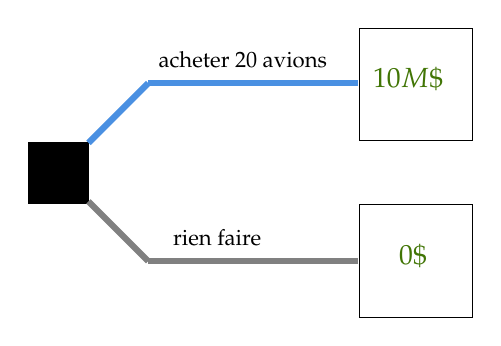
\begin{tikzpicture}[x=0.75pt,y=0.75pt,yscale=-1,xscale=1]
%uncomment if require: \path (0,173); %set diagram left start at 0, and has height of 173

%Shape: Square [id:dp24517560175499553] 
\draw  [fill={rgb, 255:red, 0; green, 0; blue, 0 }  ,fill opacity=1 ] (89.48,64.48) -- (118.52,64.48) -- (118.52,93.52) -- (89.48,93.52) -- cycle ;
%Straight Lines [id:da3756647199693315] 
\draw [color={rgb, 255:red, 74; green, 144; blue, 226 }  ,draw opacity=1 ][line width=2.25]    (147.3,35.7) -- (118.52,64.48) ;
%Straight Lines [id:da6104562133416749] 
\draw [color={rgb, 255:red, 74; green, 144; blue, 226 }  ,draw opacity=1 ][line width=2.25]    (248.3,35.7) -- (147.3,35.7) ;
%Straight Lines [id:da14739125655905938] 
\draw [color={rgb, 255:red, 128; green, 128; blue, 128 }  ,draw opacity=1 ][line width=2.25]    (147.3,121.48) -- (118.52,92.7) ;
%Straight Lines [id:da2609101791300228] 
\draw [color={rgb, 255:red, 128; green, 128; blue, 128 }  ,draw opacity=1 ][line width=2.25]    (248.3,121.48) -- (147.3,121.48) ;
%Shape: Square [id:dp3510659520557746] 
\draw   (249.25,9.25) -- (303.52,9.25) -- (303.52,63.52) -- (249.25,63.52) -- cycle ;
%Shape: Square [id:dp23837361602321772] 
\draw   (249.25,94.25) -- (303.52,94.25) -- (303.52,148.52) -- (249.25,148.52) -- cycle ;

% Text Node
\draw (151,19) node [anchor=north west][inner sep=0.75pt]  [font=\footnotesize] [align=left] {acheter 20 avions};
% Text Node
\draw (158,105) node [anchor=north west][inner sep=0.75pt]  [font=\footnotesize] [align=left] {rien faire};
% Text Node
\draw (266.89,111.89) node [anchor=north west][inner sep=0.75pt]  [color={rgb, 255:red, 65; green, 117; blue, 5 }  ,opacity=1 ] [align=left] {$\displaystyle 0\$$};
% Text Node
\draw (254.39,26.89) node [anchor=north west][inner sep=0.75pt]  [color={rgb, 255:red, 65; green, 117; blue, 5 }  ,opacity=1 ] [align=left] {$\displaystyle 10M\$$};


\end{tikzpicture}

\end{center}

Si on pose qu'il y a une chance sur deux d'avoir une forte demande, on obtient : 
\begin{center}


\tikzset{every picture/.style={line width=0.75pt}} %set default line width to 0.75pt        

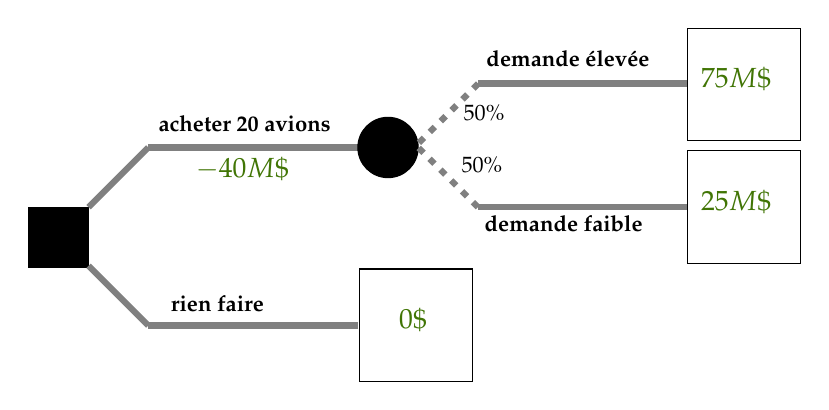
\begin{tikzpicture}[x=0.75pt,y=0.75pt,yscale=-1,xscale=1]
%uncomment if require: \path (0,231); %set diagram left start at 0, and has height of 231

%Shape: Square [id:dp32023785380502523] 
\draw  [fill={rgb, 255:red, 0; green, 0; blue, 0 }  ,fill opacity=1 ] (88.48,116.48) -- (117.52,116.48) -- (117.52,145.52) -- (88.48,145.52) -- cycle ;
%Straight Lines [id:da12822093887945507] 
\draw [color={rgb, 255:red, 128; green, 128; blue, 128 }  ,draw opacity=1 ][line width=2.25]    (146.3,87.7) -- (117.52,116.48) ;
%Straight Lines [id:da2581516742903831] 
\draw [color={rgb, 255:red, 128; green, 128; blue, 128 }  ,draw opacity=1 ][line width=2.25]    (247.3,87.7) -- (146.3,87.7) ;
%Straight Lines [id:da31217004972766316] 
\draw [color={rgb, 255:red, 128; green, 128; blue, 128 }  ,draw opacity=1 ][line width=2.25]    (146.3,173.48) -- (117.52,144.7) ;
%Straight Lines [id:da3392576403671965] 
\draw [color={rgb, 255:red, 128; green, 128; blue, 128 }  ,draw opacity=1 ][line width=2.25]    (247.3,173.48) -- (146.3,173.48) ;
%Shape: Square [id:dp170988150861471] 
\draw   (248.25,146.25) -- (302.52,146.25) -- (302.52,200.52) -- (248.25,200.52) -- cycle ;
%Shape: Circle [id:dp9895757220751431] 
\draw  [fill={rgb, 255:red, 0; green, 0; blue, 0 }  ,fill opacity=1 ] (247.3,87.7) .. controls (247.3,79.68) and (253.8,73.18) .. (261.82,73.18) .. controls (269.85,73.18) and (276.35,79.68) .. (276.35,87.7) .. controls (276.35,95.72) and (269.85,102.23) .. (261.82,102.23) .. controls (253.8,102.23) and (247.3,95.72) .. (247.3,87.7) -- cycle ;
%Straight Lines [id:da4273550651430713] 
\draw [color={rgb, 255:red, 128; green, 128; blue, 128 }  ,draw opacity=1 ][line width=2.25]  [dash pattern={on 2.53pt off 3.02pt}]  (305.3,56.93) -- (276.52,85.7) ;
%Straight Lines [id:da3703060888075631] 
\draw [color={rgb, 255:red, 128; green, 128; blue, 128 }  ,draw opacity=1 ][line width=2.25]    (406.3,56.93) -- (305.3,56.93) ;
%Straight Lines [id:da17572424004120135] 
\draw [color={rgb, 255:red, 128; green, 128; blue, 128 }  ,draw opacity=1 ][line width=2.25]  [dash pattern={on 2.53pt off 3.02pt}]  (305.12,116.48) -- (276.35,87.7) ;
%Straight Lines [id:da8780053534267966] 
\draw [color={rgb, 255:red, 128; green, 128; blue, 128 }  ,draw opacity=1 ][line width=2.25]    (406.12,116.48) -- (305.12,116.48) ;
%Shape: Square [id:dp6757137459750928] 
\draw   (406.25,30.25) -- (460.52,30.25) -- (460.52,84.52) -- (406.25,84.52) -- cycle ;
%Shape: Square [id:dp442435216663005] 
\draw   (406.25,89.25) -- (460.52,89.25) -- (460.52,143.52) -- (406.25,143.52) -- cycle ;

% Text Node
\draw (150,71) node [anchor=north west][inner sep=0.75pt]  [font=\footnotesize] [align=left] {\textbf{acheter 20 avions}};
% Text Node
\draw (156,158) node [anchor=north west][inner sep=0.75pt]  [font=\footnotesize] [align=left] {\textbf{rien faire}};
% Text Node
\draw (265.89,163.89) node [anchor=north west][inner sep=0.75pt]  [color={rgb, 255:red, 65; green, 117; blue, 5 }  ,opacity=1 ] [align=left] {$\displaystyle 0\$$};
% Text Node
\draw (167.89,91) node [anchor=north west][inner sep=0.75pt]  [color={rgb, 255:red, 65; green, 117; blue, 5 }  ,opacity=1 ] [align=left] {$\displaystyle -40M\$$};
% Text Node
\draw (411.39,47.89) node [anchor=north west][inner sep=0.75pt]  [color={rgb, 255:red, 65; green, 117; blue, 5 }  ,opacity=1 ] [align=left] {$\displaystyle 75M\$$};
% Text Node
\draw (297,66) node [anchor=north west][inner sep=0.75pt]  [font=\footnotesize] [align=left] {$\displaystyle 50\%$};
% Text Node
\draw (296,91) node [anchor=north west][inner sep=0.75pt]  [font=\footnotesize] [align=left] {$\displaystyle 50\%$};
% Text Node
\draw (308,40) node [anchor=north west][inner sep=0.75pt]  [font=\footnotesize] [align=left] {\textbf{demande élevée}};
% Text Node
\draw (307.12,119.48) node [anchor=north west][inner sep=0.75pt]  [font=\footnotesize] [align=left] {\textbf{demande faible}};
% Text Node
\draw (411.39,106.89) node [anchor=north west][inner sep=0.75pt]  [color={rgb, 255:red, 65; green, 117; blue, 5 }  ,opacity=1 ] [align=left] {$\displaystyle 25M\$$};


\end{tikzpicture}

\end{center}

\begin{itemize}
	\item	Les carrés sont des \textbf{nœuds de décisions} et les cercles des \textbf{nœuds d'information}.
	\item	Les flux financiers sont indiqués au moment qu'ils sont réalisés.
	\item	$\text{E}[\text{valeur à l'échéance}]	=	0.5 \times (75 - 40) + 0.5 \times (25 - 40)=	10$.
	\item	On peut continuer d'ajouter des possibilités et de complexifier l'arbre.
		\begin{itemize}
		\item	Par exemple, acheter 5 avions puis, si la demande est élevée, acheter 15 autres avions à un prix plus élevé de 2.2M\$ par avion.
		\item	etc.
		\end{itemize}
\end{itemize}
\end{formula}

\subsubsection{Option de calendrier}
\hl{Ajouter plus de détails et pratiquer pour bien saisir comment calculer les affaires avec Black-Scholes. Section pas complétée}.

Les options de calendrier donnent un délai à une entreprise avant d'avoir à prendre une décision. L'avantage est que la compagnie pourrait avoir davantage d'information dans le futur et réduire l'incertitude de la décision.
\begin{itemize}
	\item	On peut utiliser formule de Black Scholes.
\end{itemize}

Il y a 3 facteurs qui ont une influence sur le calendrier de l'investissement :
\begin{enumerate}
	\item	La VAN de l'investissement.
		\begin{itemize}
		\item	On investit seulement si $VAN(\text{invest. aujourd'hui}) > VAN(\text{avec une option réelle})$ $\textbf{ OU } \text{ > valeur de prendre l'option d'attendre}$.
		\item	Parfois prendre on considération l'option réelle cause une VAN négative à devenir positive.
		\end{itemize}
	\item	La volatilité.
		\begin{itemize}
		\item	La valeur d'une option d'achat augmente avec la volatilité.
		\item	Donc, attendre est la meilleur option s'il y a beaucoup d'incertitude vis-à-vis un investissement.
		\end{itemize}
	\item	Les dividendes.
		\begin{itemize}
		\item	L'équivalent des dividendes pour une option réelle sont les flux monétaires qui auxquels on renonce en attendant.
		\item	Il est souvent mieux d'attendre à moins qu'il y ait un coût associé.
		\end{itemize}
\end{enumerate}


\subsubsection{Sizing options}
\hl{Ajouter plus de détails et pratiquer comment établir les équations}.

\begin{definitionNOHFILLsub}[Options de croissance]
Lorsqu'une entreprise est optimiste pour le futur, une option de croissance lui donne l'option d'augmenter ses investissements.
\begin{itemize}
	\item	Par exemple, acheter 5 avions puis garder l'option d'en acheter 15 dans le futur si les choses vont bien.
\end{itemize}
\end{definitionNOHFILLsub}

\begin{definitionNOHFILLsub}[Options d'abandon]
Lorsqu'une entreprise est pessimiste pour le futur, une option d'abandon lui donne l'option d'abandonner un projet.
\begin{itemize}
	\item	Habituellement, elle est exercée si la VAN des flux monétaires reliés à l'abandon d'un projet sont plus élevée que ceux reliés au maintient du projet.
\end{itemize}
\end{definitionNOHFILLsub}


\pagebreak
\section{Structure du capital}
\begin{definitionNOHFILL}[Structure du capital]
Regroupe la dette et les capitaux propres qu'une entreprise utilise pour financer ses activités.
\end{definitionNOHFILL}

\subsection{Financement par actions}
\subsubsection{Financement par actions pour des compagnies privées}
\paragraph{Sources de capital}
\begin{rappel_enhanced}[Contexte]
Typiquement, lorsqu'un entrepreneur débute il obtiendra du financement à partir de sa famille et ses amis. Puis, lorsque l'entreprise commence à croître, des sources de financement externes sont nécessaires.
\end{rappel_enhanced}

\begin{definitionNOHFILLsub}[\og \textit{Angel Investors} \fg{}]
Typiquement des individus riches qui sont eux-mêmes des entrepreneurs. Ils investissent dans des compagnies et reçoivent en échange une partie des actions.
\begin{itemize}
	\item	Puisqu'il est difficile d'évaluer une entreprise à son début, les investisseurs détiennent habituellement des \og \textit{convertible notes} \fg{} en lieu d'actions.
	\item	Ces notes sont une dette à court terme qui se transforment en actions (à un rabais) lorsque la compagnie sera financée par des capitaux propres.
\end{itemize}
\end{definitionNOHFILLsub}

\begin{definitionNOHFILLsub}[\og \textit{Venture Capital Firms} \fg{}]
Lorsqu'une entreprise nécessite plus de capitaux que peuvent offrir des \og \textit{angel investors} \fg{}, elle fait appel à une \og \textit{venture capital firm} \fg{}.
\begin{itemize}
	\item	Ces \og \textit{venture capital firms} \fg{} forment des \og \textit{limited partnerships} \fg{} avec des entreprises en démarrage.
	\item	Les \og \textit{venture capital firms} requièrent habituellement beaucoup de contrôle en échange pour les fonds prêtés.
	\item	Souvent, les commanditaires sont activement impliqués dans l'entreprise et font partie du conseil d'administration.
\end{itemize}
\end{definitionNOHFILLsub}

\begin{definitionNOHFILLsub}[\og \textit{Private Equity Firms} \fg{}]
Ces entreprises sont semblables aux \og \textit{venture capital firms} \fg{} sauf qu'ils investissent dans les capitaux propres de compagnies privées. 
\begin{itemize}
	\item	Souvent, ces entreprises achètent des compagnies publiques afin de les "privatiser" dans un \og \textit{leveraged buyout (LBO)} \fg{}.
\end{itemize}
\end{definitionNOHFILLsub}

\begin{definitionNOHFILLsub}[\og \textit{Institutional Investors} \fg{}]
Par exemple, des fonds de pension, des compagnies d'assurance, des fondations, etc.
\begin{itemize}
	\item	Ils ont des gros montants d'argent à investir.
\end{itemize}
\end{definitionNOHFILLsub}

\begin{definitionNOHFILLsub}[\og \textit{Corporate Investors} \fg{}]
Des compagnies qui investissent dans d'autres compagnies privées.
\begin{itemize}
	\item	Soit pour des rendements additionnels ou pour suivre une stratégie.
\end{itemize}
\end{definitionNOHFILLsub}


\paragraph{Investissement \og \textit{Venture capital} \fg{}}
\begin{itemize}
	\item	Typiquement, lorsqu'une compagnie vend des participatifs pour la première fois, elle émet des \textbf{actions privilégiées} et non des \textbf{actions ordinaires}.
	\item	Les actions privilégiées se comportent de façon différente selon l'âge de la compagnie.
		\begin{itemize}
		\item	Des \textbf{compagnies adultes} (\og \textit{mature} \fg{}) offrent des dividendes préférentiels, une valeur en cas de liquidation ou des droits de vote avec les actions privilégiées.
		\item	Des \textbf{jeunes compagnies} offrent un droit de réclamation prioritaire aux actifs d'une compagnie dans le cas de liquidation avec les actions privilégiées.
		\end{itemize}		 
	\item	Une collecte de fonds pour une compagnie s'appelle une série de financement.
		\begin{itemize}
		\item	En ordre, on appelle les séries : \og \textit{Angel} \fg{}, \og \textit{seed round} \fg{}, $\dots$, \og \textit{IPO} \fg{}.
		\item	En anglais, \og \textit{funding round} \fg{}.
		\end{itemize}
\end{itemize}


\paragraph{Évaluation avant et après une série de financement}
Évaluation : 
\begin{description}
	\item[préfinancement]	Valeur d'une entreprise \textit{avant} une série de financement.
		\begin{itemize}
		\item	En anglais, \og \textit{pre-money valuation} \fg{}.
		\end{itemize}
	\item[après financement]	Valeur d'une entreprise \textit{après} une série de financement.
		\begin{itemize}
		\item	En anglais, \og \textit{post-money valuation} \fg{}.
		\item	Correspond à l'évaluation préfinancement + montant investit.
		\item	De façon alternative, le nombre de parts \textit{après} la série $\times$ le prix par action \textit{avant} la série.
		\end{itemize}
\end{description}

On peut trouver le \textbf{pourcentage de participation} d'un investisseur comme $\frac{\text{montant investit}}{\text{évaluation après financement}}$.
\begin{itemize}
	\item	De façon alternative, $\frac{\text{nombres d'actions détenues par l'investisseur}}{\text{nombre total d'actions}}$.
\end{itemize}


\paragraph{Conditions de financement \og \textit{Venture Capital} \fg{}}
Les distinctions principales des actions privilégiées que détiennent habituellement les \og venture capitalists \fg{} aux actions ordinaires se résument à ces caractéristiques :

\begin{definitionNOHFILLpropos}[Préférences de liquidité]
Dans le cas de liquidation d'une entreprise, un montant minimal doit être payé aux détenteurs d'actions privilégiées avant que tout paiement soit effectué aux détenteurs d'actions ordinaires.
\begin{itemize}
	\item	La préférence est trouvée par : multiplicateur $\times$ investissement initial
\end{itemize}
\end{definitionNOHFILLpropos}

\begin{definitionNOHFILLpropos}[Ancienneté]
Ceux qui investissent plus tard peuvent demander une ancienneté plus élevée que les investisseurs des séries antérieures.
\begin{itemize}
	\item	S'ils sont donnés une ancienneté égale, ils sont \textit{pari passu} (latin pour "de rang égal").
\end{itemize}
\end{definitionNOHFILLpropos}

\begin{definitionNOHFILLpropos}[Droits de participation]
Octroie les paiements payables aux détenteurs d'actions ordinaires comme si les actions auraient été converties en actions ordinaires.
\end{definitionNOHFILLpropos}

\begin{definitionNOHFILLpropos}[Protection anti-dilution]
Si une série de financement a lieu à un prix inférieur à une ronde précédente, la protection permet aux investisseurs de convertir leurs actions privilégiées en actions ordinaires à un prix inférieur.
\begin{itemize}
	\item	Ceci permet d'augmenter le pourcentage de participation des investisseurs dans l'entreprise.
\end{itemize}
\end{definitionNOHFILLpropos}

\begin{definitionNOHFILLpropos}[Participation au conseil d'administration]
Un investisseur peut tenter d'arranger la désignation d'un ou plusieurs membres au conseil d'administration.
\end{definitionNOHFILLpropos}


\paragraph{Sortie d'un investissement dans une compagnie privée}
Un investisseur a deux approches possibles :
\begin{description}
	\item[Acquisition]	D'autres investisseurs achètent les parts de l'entreprise.
	\item[Émission publique]	Avec un appel public à l'épargne (APE).
		\begin{itemize}
		\item	En anglais, \og \textit{(initial) public offering (IPO)} \fg{} pour le premier puis \og \textit{additional public offering (APO)} \fg{} pour les suivants.
		\end{itemize}
\end{description}


\subsubsection{Financement par actions pour des compagnies publiques}
Le premier APE (financement par action pour une compagnie publique) est la première fois qu'une entreprise vend ses actions au public. Il y a plusieurs avantages et désavantages pour une entreprise à devenir publique.\\

Les avantages principaux : 
\begin{itemize}
	\item	Plus de liquidité.
		\begin{itemize}
		\item	Les investisseurs qui détiennent déjà des actions de la compagnie peuvent diversifier leurs portefeuilles en vendant des actions.
		\end{itemize}
	\item	Meilleur accès à du financement.
		\begin{itemize}
		\item	Une entreprise a habituellement accès à des prêts plus importants après qu'elle devient publique.
		\end{itemize}
\end{itemize}

Les désavantages principaux :
\begin{itemize}
	\item	Détenteurs d'actions dispersés.
		\begin{itemize}
		\item	Les investisseurs ont moins de poids sur les actions de la compagnie.
		\end{itemize}
	\item	La conformité longue et coûteuse.
		\begin{itemize}
		\item	Les compagnies publiques sont sujettes à beaucoup de règlements.
		\end{itemize}
\end{itemize}


\paragraph{Types d'offres}
\begin{itemize}
	\item	Un souscripteur (\og \textit{underwriter} \fg{}) est une entreprise de services d'investissement qui gère l'appel public à l'épargne.
	\item	Il y a 2 types (principales) d'offres : 
		\begin{enumerate}
		\item	L'offre \textbf{primaire} offre des nouvelles actions.
		\item	L'offre \textbf{secondaire} offre des actions des détenteurs actuels.
		\end{enumerate}
\end{itemize}

\

Il y a plusieurs mécanismes de vente :

\begin{definitionNOHFILLpropos}[Meilleurs efforts]
Le souscripteur n'offre aucune garantie de vente des actions qui sont vendues au meilleur prix possible.
\begin{itemize}
	\item	Souvent ces ententes ont une clause tout ou rien comme quoi que l'entente est annulée s'il reste des actions qui ne sont pas vendues.
	\item	Habituellement, ce mécanisme est utilisé pour de petits APE.
\end{itemize}
\end{definitionNOHFILLpropos}

\begin{definitionNOHFILLpropos}[Vente garantie]
Le souscripteur garantit que toutes les actions seront vendues au cours vendeur.
\begin{itemize}
	\item	Approche la plus courante.
	\item	Les souscripteurs achètent les actions avec un rabais puis tentent de les revendre au cours vendeur.
	\item	Le souscripteur assume le risque qu'elles se vendent pour moins cher.
	\item	Pour cette raison, ils vont souvent sous-évaluer le prix d'une action pour une vente garantie.
\end{itemize}
\end{definitionNOHFILLpropos}

\begin{definitionNOHFILLpropos}[Vente aux enchères]
Les actions se vendent à un même prix aux investisseurs les plus offrants afin qu’elles soient toutes vendues.
\end{definitionNOHFILLpropos}


\paragraph{Mécanisme de l'APE}
\begin{itemize}
	\item	Un groupe de souscripteurs gère l'APE avec un souscripteur principal.
		\begin{itemize}
		\item	Les plus petits souscripteurs reçoivent (\og \textit{syndicates} \fg{}) des conseils du souscripteur principal.
		\end{itemize}
	\item	Les entreprises doivent déposer une déclaration d'enregistrement à la commission réglementaire.
	\item	La déclaration a 2 composantes principales :
		\begin{enumerate}
		\item	Prospectus provisoire avec l'information nécessaire aux investisseurs potentiels.
		\item	Prospectus définitif avec des détails sur l'APE (quantité d'actions disponibles, prix, etc.)
		\end{enumerate}
	\item	Une évaluation de la compagnie est effectuée par le souscripteur.
		\begin{itemize}
		\item	Souvent, la valeur est établie selon la VAN des flux monétaires ou la valeur de compagnies semblables.
		\item	Habituellement, l'entreprise a une conférence avec les clients les plus importants du souscripteur pour vendre l'entreprise.
		\item	Par la suite, le souscripteur ajuste le prix de l'action selon a demande perçue pour maximiser la probabilité de succès (\og \textit{book building} \fg{}).
		\end{itemize}
	\item	L'entreprise paye au souscripteur l'écart de souscription (\og \textit{underwriting spread} \fg{}).
		\begin{itemize}
		\item	Ceci est un pourcentage du prix d'émission.
		\item	P. ex., 5\% sur un prix de 10\$ engendre des frais de 0.5\$ par action permettant le souscripteur d'acheter l'action pour 9.50\$ puis de la vendre pour 10\$.
		\end{itemize}
	\item	Le souscripteur gère son risque.
%%%	------------------------
%%%	NOTES
%%%	+	Pas clair ceci, faut améliorer.
%%%	------------------------
		\begin{itemize}
		\item	Un souscripteur peut se protéger contre pertes avec une option d'attribution excédentaire (\og \textit{over-allotmentt} \fg{}) ou de couverture (\og \textit{greenshoe} \fg{}).
		\item	Ces options permettent au souscripteur d'émettre un nombre limité d'options additionnelles au cours vendeur.
		\end{itemize}
\end{itemize}


\paragraph{Énigmes d'APE}
Quatre aspects de l'APE sont un mystère aux économistes financiers :

\begin{definitionNOHFILLpropos}[Sous-évaluation]
En moyenne, le prix d'émission d'un APE est trop faible.

\begin{itemize}
	\item	En partie, ceci est puisque les souscripteurs souhaitent minimiser leur risque.
	\item	Ceci cause les rendements d'un APE à être anormalement positifs.
	\item	La sous-évaluation est avantageuse pour les souscripteurs et les investisseurs qui achètent directement des souscripteurs, mais mauvaise pour l'entreprise et les investisseurs qui détiennent des actions avant l'émission.
\end{itemize}
\end{definitionNOHFILLpropos}

\begin{definitionNOHFILLpropos}[Cycles]
Les nouvelles émissions semblent cycliques.
\begin{itemize}
	\item	Le nombre d'APE n'est pas seulement influencé par le besoin de capitaux propres (alias, en temps de crise).
\end{itemize}
\end{definitionNOHFILLpropos}

\begin{definitionNOHFILLpropos}[Coût d'un APE]
Les coûts de transaction d'un APE sont élevés.
\begin{itemize}
	\item	Les frais ne semblent pas d'être variables selon la taille de l'émission.
	\item	Les souscripteurs avec légèrement moins de frais ont tendance à avoir une plus grande portion du marché que les souscripteurs avec beaucoup moins de frais.
\end{itemize}
\end{definitionNOHFILLpropos}

\begin{definitionNOHFILLpropos}[Performance à long terme]
En moyenne, la performance à long terme suite à un APE n'est pas bonne.
\end{definitionNOHFILLpropos}


\columnbreak
\subsection{Financement par emprunt}
\subsubsection{Dette corporative}
Une entreprise finance ses activités avec des capitaux propres et de la dette. Des obligations émises par des entreprises sont nommées des \textbf{\textit{obligations corporatives}} dont il y a deux types : publique et privée.

\paragraph{Dette publique} Dette transigée en bourse.

\begin{definitionNOHFILL}[Fiducie]
Entente légale entre l'émetteur de la dette et une société fiduciaire.
\begin{itemize}
	\item	La société défend les intérêts des détenteurs de l'obligation.
	\item	Elle s'assure que l'entreprise reste conforme aux conditions de la fiducie.
\end{itemize}
\end{definitionNOHFILL}

\

Il y a 4 types de dettes corporatives courants : des billets, des débentures, des obligations hypothécaires et des titres adossés d'actifs. Ces types tombent dans l'une des deux catégories suivantes : 

\begin{definitionNOHFILLprop}[Dette non garantie]
Dans le cas d'une faillite, les détenteurs de la dette ont seulement recours aux actifs qui ne sont pas réclamés comme garantie à d'autres dettes.

\begin{itemize}
	\item	Par exemple, des billets et débentures.
	\item	En anglais, \og \textit{unsecured debt} \fg{}.
\end{itemize}
\end{definitionNOHFILLprop}

\begin{definitionNOHFILLprop}[Dette garantie]
Dans le cas d'une faillite, les détenteurs ont le droit à des actifs spécifiques qui ont été désignés comme garantie.

\begin{itemize}
	\item	Par exemple, des obligations hypothécaires et des titres adossés d'actifs.
	\item	En anglais, \og \textit{secured debt} \fg{}.
\end{itemize}
\end{definitionNOHFILLprop}

\

Le niveau d'ancienneté d'une obligation corporative indique la priorité d'un détenteur dans la réclamation d'actifs.
\begin{itemize}
	\item	Typiquement, les détenteurs de débentures imposent une clause empêchant l'entreprise d'émettre des dettes avec une priorité plus élevée.
	\item	Ces dettes qui sont moins prioritaires sont nommées des débentures subordonnées.
\end{itemize}

\

Les obligations internationales ont 4 catégories générales :
\begin{definitionNOHFILLprop}[Obligations intérieures]
Obligations émises par une entité interne avec une devise interne qui sont achetées par des investisseurs étrangers.
\begin{itemize}
	\item	En anglais, \og \textit{domestic bonds} \fg{}.
\end{itemize}
\end{definitionNOHFILLprop}

\begin{definitionNOHFILLprop}[Obligations étrangères]
Obligations émises par une entité étrangère avec une \textit{devise interne} qui sont achetées par des investisseurs locaux dans un marché interne.
\begin{itemize}
	\item	En anglais, \og \textit{foreign bonds} \fg{}.
\end{itemize}
\end{definitionNOHFILLprop}

\begin{definitionNOHFILLprop}[Euro-obligations]
Obligations dont la devise n'est pas celle du pays d'origine pouvant être transigé n'importe où et émis par une entité interne ou étrangère.
\begin{itemize}
	\item	En anglais, \og \textit{eurobonds} \fg{}.
\end{itemize}
\end{definitionNOHFILLprop}
\begin{definitionNOHFILLprop}[Obligations multimarchés]
Obligations vendues sur plusieurs marchés en même temps.
\begin{itemize}
	\item	En anglais, \og \textit{global bonds} \fg{}.
\end{itemize}
\end{definitionNOHFILLprop}


\paragraph{Dette privée}	Dette négociée directement avec une banque ou un petit groupe d'investisseurs.
\begin{itemize}
	\item	L'avantage est que l'émission est moins coûteuse puisqu'il n'y a pas de frais.
	\item	Le désavantage est que le marché n'est pas liquide.
\end{itemize}

\

Il y a 2 types principaux de dette privée: 

\begin{definitionNOHFILLpropos}[Prêt à terme]
Emprunt d'une banque pour une période de temps fixée.
\begin{itemize}
	\item	Si plusieurs banques financent un même prêt, c'est un \og \textit{syndicated bank loan} \fg{}.
\end{itemize}
\end{definitionNOHFILLpropos}

\begin{definitionNOHFILLpropos}[Émission privée]
Émission d'obligations à un petit groupe d'investisseurs directement.
\begin{itemize}
	\item	Cette émission est moins restrictive qu'un prêt à terme.
\end{itemize}
\end{definitionNOHFILLpropos}


\subsubsection{Autres}
\paragraph{Obligations émises par des gouvernements}	Les gouvernement émettent de la dette pour financer leurs projets.

\begin{definitionNOHFILLprop}[Dette souveraine]
Dette émise par le gouvernement national nommées des "titres du trésor".\\

Il y a 4 types de titres du trésor :
\begin{description}
	\item[Bon du trésor]	Obligation \textbf{zéro coupon} avec une \textbf{échéance de moins d'un an}.
	\item[Certificat du trésor]	Obligation avec des \textbf{coupons semestriels} et une \textbf{échéance de 1 à 10 ans}.
	\item[Obligation du trésor]		Obligations avec des \textbf{coupons semestriels} et une \textbf{échéance au-dessus de 10 ans}.
	\item[Titre du trésor protégé contre l'inflation]	Obligation avec des \textbf{coupons semestriels} dont \textbf{le capital et le paiement} sont \textbf{ajustés pour l'inflation}.
\end{description}
\end{definitionNOHFILLprop}

\begin{definitionNOHFILLprop}[Obligations municipales]
Dette émise par des gouvernements provinciales (de l'état aux É.-U.) ou municipales.

\begin{itemize}
	\item	Habituellement, les rendements sont libres d'impôts fédérales.
	\item	Le taux peut être fixe ou variable.
	\item	Le taux de défaillance des ses obligations est plus élevée que les obligations fédérales à environ 4\% depuis 1970 aux É.-U.
\end{itemize}

\

Il y a quelques types dont des obligations : 
\begin{description}
	\item[Spécifiques]	Les rendements proviennent d'un projet en particulier de la ville pour lequel il faut lever des fonds.
		\begin{itemize}
		\item	En anglais, \og \textit{revenue bonds} \fg{}.
		\end{itemize}
	\item[À caractère général]	Les rendements sont adossés par la ville.
		\begin{itemize}
		\item	En anglais, \og \textit{general obligation bonds} \fg{}.
		\end{itemize}
\end{description}
\end{definitionNOHFILLprop}

\paragraph{Note}	Il est important de savoir que les sécurités financières (e.g., \og \textit{t-bills} \fg{}) ont des coupons semi-annuels et de le considérer dans des questions relatives aux coupons.


\paragraph{Titres adossés à des actifs}
%%%	------------------------
%%%	NOTES
%%%	+	Manque de détails.
%%%	------------------------
\begin{definitionNOHFILL}[Titre adossé à des actifs]
Titre dont les rendements proviennent d'actifs sous-jacent.

\begin{itemize}
	\item	Par exemple, les titres adossés à des créances hypothécaires (\og \textit{mortgage-backed securities (MBS)} \fg{}).
	\item	Également, des MBS peuvent être adossés à d'autres MBS (\og \textit{collateralized debt obligation (CDO)} \fg{}).
	\item	En anglais, \og \textit{asset-backed security (ABS)} \fg{}.
\end{itemize}
\end{definitionNOHFILL}


\columnbreak
\subsection{Propositions de Modigliani-Miller}
\begin{distributions}[Notation]
\begin{description}
	\item[$U$]	Valeur au marché de l'équité d'une entreprise sans levier.
	\item[$E$]	Valeur au marché de l'équité d'une entreprise avec levier.
	\item[$D$]	Valeur au marché de la dette d'une entreprise avec levier.
	\item[$V_{U}$]	Valeur au marché d'une entreprise sans levier.
		\begin{itemize}
		\item	\lfbox[formula]{$V_{U}	=	U$}.
		\end{itemize}
	\item[$V_{L}$]	Valeur au marché d'une entreprise avec levier.
		\begin{itemize}
		\item	\lfbox[formula]{$V_{L}	=	E	+	D$}.
		\end{itemize}
\end{description}
\end{distributions}

\subsubsection{Proposition I (sans impôts)}
\textbf{La structure du capital n'a aucun impact sur la valeur d'une entreprise} sous les conditions suivantes :
\begin{definitionNOHFILLpropos}[Conditions pour la proposition 1 de MM]
\begin{enumerate}
	\item	Tous les investisseurs ont les mêmes attentes de rendements.
	\item	Les marchés financiers sont parfaitement concurrentiels.
		\begin{itemize}
		\item	Concept de micro.
		\item	En anglais, \og \textit{perfect competition} \fg{}.
		\item	Il n'y a pas de taxes, de frais de transaction, de coûts de faillite.
		\end{itemize}
	\item	Les investisseurs peuvent emprunter et prêter au taux sans risque.
	\item	Il n'y a pas de conflits d'intérêts entre les gestionnaires et les actionnaires (aucun coût d'agence).
		\begin{itemize}
		\item	Les gestionnaires agissent dans le meilleur intérêt des actionnaires.
		\end{itemize}
	\item	Les décisions d'investissement et de financement d'une entreprise sont indépendantes.
		\begin{itemize}
		\item	C'est-à-dire que les décisions de financement n’ont aucune influence sur les revenus que génèrent les investissements.
		\end{itemize}
\end{enumerate}
\end{definitionNOHFILLpropos}

Donc, la structure du capital d'une entreprise n'a aucune importance à sa valeur. 
\begin{itemize}
	\item	Selon MM I, une compagnie composée à 75\% de capitaux propres et 25\% de dette est équivalente à une entreprise composée à 75\% de dette et à 25\% de capitaux propres. 
	\item	C'est à dire, $V_{L}	=	V_{U}$.
	\item	Un investisseur peut augmenter ou diminuer le levier de son portefeuille aux taux sans risque (condition 3) et donc obtenir une structure de capital à son goût sans égard.
		\begin{itemize}
		\item	La structure de l'entreprise dans laquelle il investit n'a donc aucun impact sur sa décision d'investir.
		\item	En anglais, ceci s'appelle du \og \textit{homemade leverage} \fg{}.
		\end{itemize}
\end{itemize}


\subsubsection{Proposition II de MM (sans impôts)}
\begin{itemize}
	\item	Nous \hyperref[sec:wacc_def]{\textcolor{teal}{avons vu}} que \lfbox[rappel]{$r_{CMPC}	=	\frac{E}{E + D} r_{E} + \frac{D}{E + D} r_{D}$}.
	\item	Également, puisque sous la proposition I de MM \lfbox[conditions]{$V_{U}	=	V_{L}$} alors \lfbox[formula]{$U	=	E + D$}.
	\item	Sans impôts, on trouve que le CMPC et le coût du capital sans levier sont égaux : $r_{U}	=	r_{CMPC}$. 
	\item	En réécrivant l'équation, \lfbox[formula]{$r_{E}	=	r_{U} + \frac{D}{E} (r_{U}	-	r_{D})$}.
\end{itemize}

On voit donc qu'une augmentation de la dette $D$ augmente le rendement sur les capitaux propres avec levier $r_{E}$.
\begin{itemize}
	\item	La préposition 2 de MM stipule que \textbf{le coût des capitaux propres avec levier augmente avec le ratio d'endettement d'une entreprise}.
\end{itemize}

%%%	------------------------
%%%	NOTES
%%%	+	Mieux expliquer ceci intuitivement (AJvR).
%%%	------------------------
\

\begin{itemize}
	\item	Initialement, le coût de la dette est plus faible que celui des capitaux propres puisque les rendements sont plus faibles et moins risqués. 
	\item	Cependant, plus une entreprise a de la dette plus le risque que les actionnaires ne se fassent pas payer augmente. 
	\item	Alors, le coût croissant des capitaux propres contrebalance l'avantage d'utiliser davantage de dette ce qui mène à un CMPC constant.
	\item	Visuellement : 
\end{itemize}
\begin{center}
\tikzset{every picture/.style={line width=0.75pt}} %set default line width to 0.75pt        

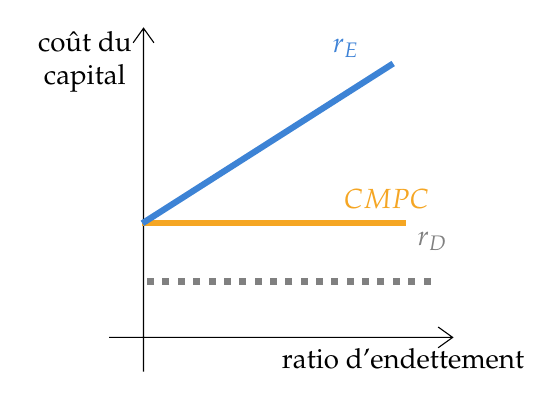
\begin{tikzpicture}[x=0.75pt,y=0.75pt,yscale=-1,xscale=1]
%uncomment if require: \path (0,208); %set diagram left start at 0, and has height of 208

%Shape: Axis 2D [id:dp8697465826041249] 
\draw  (102,180.95) -- (267.5,180.95)(118.55,32) -- (118.55,197.5) (260.5,175.95) -- (267.5,180.95) -- (260.5,185.95) (113.55,39) -- (118.55,32) -- (123.55,39)  ;
%Straight Lines [id:da8814727713420509] 
\draw [color={rgb, 255:red, 245; green, 166; blue, 35 }  ,draw opacity=1 ][line width=2.25]    (244.83,126) -- (118,126) ;
%Straight Lines [id:da16442005234532675] 
\draw [color={rgb, 255:red, 61; green, 131; blue, 213 }  ,draw opacity=1 ][line width=2.25]    (238.83,49) -- (118,126) ;
%Straight Lines [id:da9188413160436577] 
\draw [color={rgb, 255:red, 128; green, 128; blue, 128 }  ,draw opacity=1 ][line width=2.25]  [dash pattern={on 2.53pt off 3.02pt}]  (256.83,154) -- (118,154) ;

% Text Node
\draw (184,185) node [anchor=north west][inner sep=0.75pt]   [align=left] {ratio d'endettement};
% Text Node
\draw (63,32) node [anchor=north west][inner sep=0.75pt]   [align=left] {\begin{minipage}[lt]{39.015pt}\setlength\topsep{0pt}
\begin{center}
coût du \\capital
\end{center}

\end{minipage}};
% Text Node
\draw (206,36) node [anchor=north west][inner sep=0.75pt]   [align=left] {\begin{minipage}[lt]{13.175pt}\setlength\topsep{0pt}
\begin{center}
\textcolor[rgb]{0.24,0.51,0.84}{$\displaystyle r_{E}$}
\end{center}

\end{minipage}};
% Text Node
\draw (246.83,129) node [anchor=north west][inner sep=0.75pt]   [align=left] {\begin{minipage}[lt]{14.527928000000001pt}\setlength\topsep{0pt}
\begin{center}
\textcolor[rgb]{0.24,0.51,0.84}{$\displaystyle \textcolor[rgb]{0.5,0.5,0.5}{r_{D}}$}
\end{center}

\end{minipage}};
% Text Node
\draw (209.83,108) node [anchor=north west][inner sep=0.75pt]   [align=left] {\begin{minipage}[lt]{36.6775pt}\setlength\topsep{0pt}
\begin{center}
\textcolor[rgb]{0.24,0.51,0.84}{$\displaystyle \textcolor[rgb]{0.96,0.65,0.14}{CMPC}$}
\end{center}

\end{minipage}};


\end{tikzpicture}

\end{center}

\begin{formula}{Exemple de calcul du CMPC et du coût des capitaux propres sans effet de levier}
Soit la compagnie LMN qui veut changer sa structure de capital pour avoir un ratio d'endettement ($D/E$) de $0.75$.
\begin{itemize}
	\item	Le ratio d'endettement ($D/E$) d'LMN est présentement de $0.50$.
	\item	Le coût des capitaux d'emprunt ($r_{D}$) est présentement de $7\%$.
	\item	Le coût des capitaux propres ($r_{E}$) est présentement de $11.5\%$.
	\item	Augmenter le ratio ratio d'endettement ($D/E$) d'LMN à $0.75$ augmente le coût des capitaux d'emprunt à $9\%$.
\end{itemize}

On trouve le CMPC, et donc le coût des capitaux propres sans effet de levier $r_{U}$, avec $r_{CMPC}	=	r_{U}	=	\frac{0.5E}{1.5E} r_{E} + \frac{1E}{1.5E} r_{D}	=	\frac{1}{3} \times 0.115 + \frac{2}{3} \times 0.07	=	0.10$.\\

Avec $r_{U}	=	10\%$, on trouve que le coût des capitaux propres avec effet de levier est $r_{E}^{\ast}	=	r_{U}	+	\frac{D}{E} (r_{U}	-	r_{D}^{\ast})	=	0.10 + 0.75 (0.10 - 0.09)	=	0.1075$.
\end{formula}


\paragraph{CMPC avec plusieurs titres}	Les deux types de titres qui forment typiquement la structure du capital d'une entreprise sont les capitaux propres et la dette. 
\begin{itemize}
	\item	Si une compagnie a plus de titres, il suffit de faire une moyenne pondérée des rendements. 
	\item	Pour $n$ types de rendements \lfbox[formula]{$r_{U}	=	\sum_{i	=	1}^{n} w_{i} r_{i}$}.
	\item	Par exemple, elle pourrait avoir des actions ordinaires et des actions privilégiées.
\end{itemize}


\paragraph{Betas avec et sans effet de levier}	On peut appliquer la formule du coût des capitaux propres sans effet de levier aux betas avec $\beta_{E}	=	\beta_{U} + \frac{D}{E}(\beta_{U}	-	\beta_{D})$ qui découle de l'équation $\beta_{U}	=	w_{E} \beta_{E} + w_{D} \beta_{D}$.


\subsubsection{Propositions avec impôts}
\paragraph{Proposition I de MM}	Avec impôt, la structure du capital a un impact sur la valeur d'une entreprise puisque les paiements d'intérêt sont habituellement réductibles d'impôts.
\begin{itemize}
	\item	Emprunter offre donc des épargnes qui augmentent la valeur d'une entreprise.
	\item	On trouve que $$V_{L}		=	V_{U} + \shortstack{bouclier fiscale\\ sur l'intérêt}$$
	\item	Également, $$\shortstack{bouclier fiscale\\ sur l'intérêt}	=	\tau_{C} \times \text{paiements d'intérêt}$$
\end{itemize}

\begin{formula}{Exemple de la valeur d'une entreprise avec effet de levier}
Soit :
\begin{itemize}
	\item	un emprunt de $2M\$$ avec intérêt de $10\%$ par année.
	\item	un taux d'imposition $\tau_{C}	=	45\%$.
	\item	un taux sans risque $r_{f}	=	5\%$.
\end{itemize}

La compagnie décide de payer l'intérêt a chaque année puis de payer le principal à la fin de 10 ans.\\

Alors, le bouclier fiscale est de $0.45 \times 2M \times 0.10	=	900k\$$ par année. 
\begin{itemize}
	\item	La valeur actualisée est $900k\$ \ax{\angl{10}5\%}	=	6.9M\$$. 
	\item	Alors, $V_{L}	=	V_{U}	+	6.9M\$$.
\end{itemize}
\end{formula}

\paragraph{Proposition II de MM}	Le CMPC après impôts calcule le coût des capitaux propres en considérant l'avantage du bouclier fiscale.

On trouve donc que \lfbox[formula]{$r_{CMPC}	=	w_{E} r_{E} + w_{D} r_{D} (1 - \tau_{C})$} ou de façon équivalente : 
\begin{align*}
	\underbrace{w_{E} r_{E} + w_{D} r_{D}}_{\text{CMPC avant impôts}} - \underbrace{\tau_{C} w_{D} r_{D}}_{\text{bouclier fiscale}}
\end{align*}

\

Également, le coût des capitaux propres avec effet de levier est \lfbox[formula]{$r_{E}	=	r_{U} + \frac{D}{E} (r_{U} - r_{D})(1 - \tau_{C})$}.

Visuellement : 
\begin{center}
\tikzset{every picture/.style={line width=0.75pt}} %set default line width to 0.75pt        

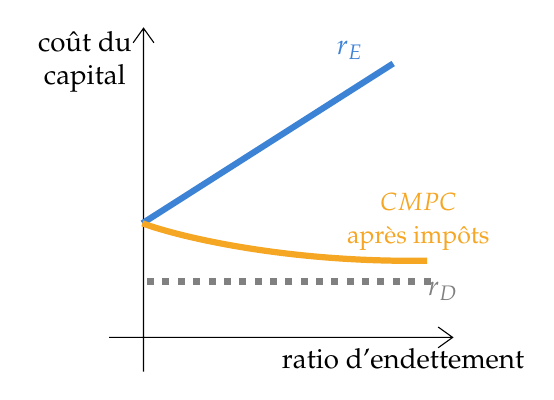
\begin{tikzpicture}[x=0.75pt,y=0.75pt,yscale=-1,xscale=1]
%uncomment if require: \path (0,208); %set diagram left start at 0, and has height of 208

%Shape: Axis 2D [id:dp05665703449666082] 
\draw  (102,180.95) -- (267.5,180.95)(118.55,32) -- (118.55,197.5) (260.5,175.95) -- (267.5,180.95) -- (260.5,185.95) (113.55,39) -- (118.55,32) -- (123.55,39)  ;
%Straight Lines [id:da23527423296147232] 
\draw [color={rgb, 255:red, 61; green, 131; blue, 213 }  ,draw opacity=1 ][line width=2.25]    (238.83,49) -- (118,126) ;
%Straight Lines [id:da33774173673680163] 
\draw [color={rgb, 255:red, 128; green, 128; blue, 128 }  ,draw opacity=1 ][line width=2.25]  [dash pattern={on 2.53pt off 3.02pt}]  (256.83,154) -- (118,154) ;
%Curve Lines [id:da600116537886787] 
\draw [color={rgb, 255:red, 245; green, 166; blue, 35 }  ,draw opacity=1 ][line width=2.25]    (118,126) .. controls (137.17,133) and (189.17,145) .. (255.17,144) ;

% Text Node
\draw (184,185) node [anchor=north west][inner sep=0.75pt]   [align=left] {ratio d'endettement};
% Text Node
\draw (63,32) node [anchor=north west][inner sep=0.75pt]   [align=left] {\begin{minipage}[lt]{39.015pt}\setlength\topsep{0pt}
\begin{center}
coût du \\capital
\end{center}

\end{minipage}};
% Text Node
\draw (208,37) node [anchor=north west][inner sep=0.75pt]   [align=left] {\begin{minipage}[lt]{13.175pt}\setlength\topsep{0pt}
\begin{center}
\textcolor[rgb]{0.24,0.51,0.84}{$\displaystyle r_{E}$}
\end{center}

\end{minipage}};
% Text Node
\draw (251.83,153) node [anchor=north west][inner sep=0.75pt]   [align=left] {\begin{minipage}[lt]{14.527928000000001pt}\setlength\topsep{0pt}
\begin{center}
\textcolor[rgb]{0.24,0.51,0.84}{$\displaystyle \textcolor[rgb]{0.5,0.5,0.5}{r}\textcolor[rgb]{0.5,0.5,0.5}{_{D}}$}
\end{center}

\end{minipage}};
% Text Node
\draw (212.83,110) node [anchor=north west][inner sep=0.75pt]   [align=left] {\begin{minipage}[lt]{55.27835600000001pt}\setlength\topsep{0pt}
\begin{center}
{\small \textcolor[rgb]{0.24,0.51,0.84}{$\displaystyle \textcolor[rgb]{0.96,0.65,0.14}{CMPC}$}\textcolor[rgb]{0.96,0.65,0.14}{ }}\\\textcolor[rgb]{0.96,0.65,0.14}{{\small après impôts}}
\end{center}

\end{minipage}};


\end{tikzpicture}
\end{center}


\columnbreak
\subsubsection{Coûts de détresse financière}
\hl{Ajouter plus de détails et pratiquer pour bien saisir comment calculer les VAN. Section pas complétée}.
Le désavantage des leviers financiers est les pertes importantes qu'ils causent en temps de crises.

La valeur actualisée des coûts de détresse financière a 3 composantes : 
\begin{enumerate}
	\item	Les coûts liés à une détresse financière et une faillite s'il y a une détresse.
		\begin{itemize}
		\item	Ceux-ci peuvent être des coûts :
		\begin{description}
		\item[directs]	Des dépenses encourues en lien avec la faillite (p. ex., des frais judiciaires et administratifs).
		\item[indirects]	Inclus les opportunités de placement perdues, perte d'affaires, etc.
			\begin{itemize}
			\item	Ces coûts sont plus difficiles à quantifier et sont habituellement plus importants que les coûts directs.
			\end{itemize}
		\end{description}
		\end{itemize}
%%%	------------------------
%%%	NOTES
%%%	+	Vraiment pas clair ici (AJvR).
%%%	------------------------
	\item	Le probabilité qu'une détresse financière ait lieu.
		\begin{itemize}
		\item	Ceci augmente avec le ratio d'endettement.
		\item	Également, elle augmente avec la volatilité des rendements. 
		\end{itemize}
	\item	Le rabais pour les coûts de détresse.
		\begin{itemize}
		\item	Le rabais varie selon le risque au marché de l'entreprise.
		\item	Plus le beta d'une entreprise est élevé, plus la probabilité qu'elle soit en détresse est élevée et plus son beta des coûts de détresse est négatif.
		\item	Plus un beta est négatif, plus le coût du capital décroît et par conséquent la valeur actualisée des coûts de détresse augmente.
		\end{itemize}
\end{enumerate}


\subsubsection{Coûts et avantages de \og \textit{agency costs} \fg{}}
\hl{Ajouter plus de détails et pratiquer pour bien saisir. J'étais tanné et j'ai moins bien fait cette section qui n'est pas complétée}.

La structure du capital peut influencer les décisions d'investissement des gestionnaires. 
\begin{definitionNOHFILL}[\og \textit{agency costs} \fg{}]
Coûts liés au conflits d'intérêt parmi les parties prenantes de l'entreprise (gestionnaires, actionnaires et créanciers). 
\begin{itemize}
	\item	C'est le problème qui survient en raison du partage inégale des coûts et des avantages des actions de l'entreprise.
\end{itemize}
\end{definitionNOHFILL}

%%%	------------------------
%%%	NOTES
%%%	+	Distinguer les agency costs des agency benefits (AJvR).
%%%	------------------------

\paragraph{Coûts comme levier}	L'utilisation d'un levier financier par une entreprise implique un conflit d'intérêts si les décisions d'investissement ont des conséquences différentes pour les actionnaires et les créanciers.

P. ex. : 
\begin{itemize}
	\item	Prise de risque excessive et remplacement d'actifs.
		\begin{itemize}
		\item	Une entreprise qui remplace ses actifs à risque faible par des actifs très risqués engendre le problème de remplacement d'actifs.
		\item	Le rendement des actionnaires est lié à la performance de l'entreprise et donc ils préfèrent des investissements risqués avec un potentiel de rendements plus élevés.
		\item	Les créanciers ont des revenus fixes et donc préfèrent des investissements moins risqués.
		\end{itemize}
	\item	Excédent de dette ou sous-investissement.
		\begin{itemize}
		\item	En cas de faillites, les créanciers se font payer avec les actionnaires.
		\item	Les actionnaires pourrait donc ne pas financer des projets avec une VAN positive qui seraient majoritairement avantageux pour les créanciers. 
		\end{itemize}
	\item	Retrait d'investissement.
		\begin{itemize}
		\item	Les actionnaires ont un incitatif à vendre les actifs pour des prix inférieurs à leur valeur puisqu'ils seront payés après les créanciers.
		\end{itemize}
\end{itemize}


\paragraph{Avantages comme levier}
Les gestionnaires peuvent avoir des motivations qui diffèrent des actionnaires et des créanciers, p. ex. : 
\begin{description}
	\item[\og \textit{empire building} \fg{}]	Les gestionnaires sans participation au capital peuvent choisir des projets avec un VAN négative.
		\begin{itemize}
		\item	Ils préfèrent être gestionnaires pour des grosses compagnies et donc choisissent des projets qui augmentent la taille de l'entreprise même si ceux-ci diminuent la rentabilité.
		\end{itemize}
	\item[\og \textit{managerial entrenchment} \fg{}]	Puisqu'il est peu probable que les gestionnaires soient remplacés, ils peuvent décider de faire ce qu'ils veulent.
		\begin{itemize}
		\item	Il s'ensuit qu'ils peuvent prendre des décisions qui sont avantageuses pour eux, et non les actionnaires.
		\end{itemize}
\end{description}

Les leviers peuvent aussi motiver les gestionnaires à diriger l'entreprise d'une façon plus efficace en raison de : 
\begin{itemize}
	\item	La concentration accrue des actionnaires.
		\begin{itemize}
		\item	Les gestionnaires ayant une plus grosse participation dans l'entreprise ont plus d'incitatifs à prendre les meilleurs décisions pour l'entreprise.
		\end{itemize}
	\item	La diminution des dépenses inutiles.
		\begin{itemize}
		\item	Moins de levier implique moins d'argent à dépenser et donc moins de dépends inutiles (\og \textit{free cash flow hypothesis} \fg{}).
		\end{itemize}
	\item	Diminution du \og \textit{managerial entrenchment} \fg{} et engagement accru.
		\begin{itemize}
		\item	Il est plus probable qu'un gestionnaire soit renvoyé en détresse financière.
		\item	Donc, les gestionnaires sont plus motivés à diminuer le levier et donc la probabilité de détresse financière.
		\end{itemize}
\end{itemize}


\subsubsection{Coûts d'information asymétrique}
Il y a de l'\textbf{information asymétrique} lorsque les gestionnaires ont plus d'information sur l'entreprise que les actionnaires.

Signales

\begin{itemize}
	\item	Émettre des actions est typiquement vu comme un signal négatif
	\item	Emprunter de l'argent est typiquement vu comme un signal positif
\end{itemize}

\og \textit{pecking order hypothesis} \fg{}


\subsubsection{Théorie de l'arbitrage}
Cherche à balancer les effets qui augmente la valeur de la compagnie avec la dette (bouclier fiscale, \og \textit{agency benefits} \fg{}) avec les effet qui diminuent la valeur de la compagnie (détresse financière, \og \textit{agency costs} \fg{}).

\begin{itemize}
	\item	En anglais, \og \textit{trade-off theory} \fg{}.
\end{itemize}

Selon la théorie : 
\begin{align*}
	V_{L}
	&=	V_{U} 
		+ VAN(\text{bouclier fiscale sur l'intérêt})
	 	- VAN(\text{coûts de détresse financière})
	 	- VAN(\text{\og \textit{agency costs} \fg{} de la dette})
	 	+ VAN(\text{\og \textit{agency benefits} \fg{} de la dette})
\end{align*}

Visuellement : 

\begin{center}
\tikzset{every picture/.style={line width=0.75pt}} %set default line width to 0.75pt        

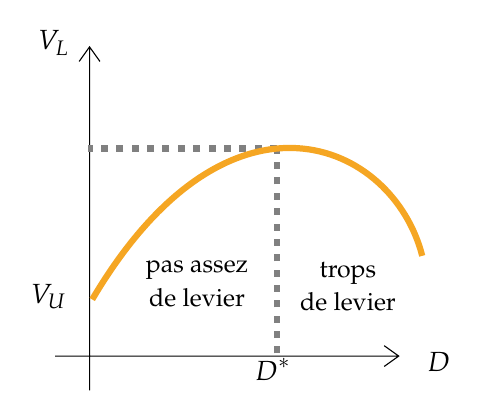
\begin{tikzpicture}[x=0.75pt,y=0.75pt,yscale=-1,xscale=1]
%uncomment if require: \path (0,208); %set diagram left start at 0, and has height of 208

%Shape: Axis 2D [id:dp05665703449666082] 
\draw  (102,180.95) -- (267.5,180.95)(118.55,32) -- (118.55,197.5) (260.5,175.95) -- (267.5,180.95) -- (260.5,185.95) (113.55,39) -- (118.55,32) -- (123.55,39)  ;
%Straight Lines [id:da33774173673680163] 
\draw [color={rgb, 255:red, 128; green, 128; blue, 128 }  ,draw opacity=1 ][line width=2.25]  [dash pattern={on 2.53pt off 3.02pt}]  (208.83,81) -- (118,81) ;
%Straight Lines [id:da046646595883229836] 
\draw [color={rgb, 255:red, 128; green, 128; blue, 128 }  ,draw opacity=1 ][line width=2.25]  [dash pattern={on 2.53pt off 3.02pt}]  (208.83,179.67) -- (208.83,81) ;
%Curve Lines [id:da9219069987832074] 
\draw [color={rgb, 255:red, 245; green, 166; blue, 35 }  ,draw opacity=1 ][line width=2.25]    (119.83,153.67) .. controls (185.67,42.33) and (264.83,77.67) .. (278.83,132.67) ;

% Text Node
\draw (280,178) node [anchor=north west][inner sep=0.75pt]   [align=left] {$\displaystyle D$};
% Text Node
\draw (89,23) node [anchor=north west][inner sep=0.75pt]   [align=left] {\begin{minipage}[lt]{16.575000000000003pt}\setlength\topsep{0pt}
\begin{center}
$\displaystyle V_{L}$
\end{center}

\end{minipage}};
% Text Node
\draw (197,181) node [anchor=north west][inner sep=0.75pt]   [align=left] {$\displaystyle D^{*}$};
% Text Node
\draw (89,145) node [anchor=north west][inner sep=0.75pt]   [align=left] {$\displaystyle V_{U}$};
% Text Node
\draw (138,134) node [anchor=north west][inner sep=0.75pt]   [align=left] {\begin{minipage}[lt]{46.60835600000001pt}\setlength\topsep{0pt}
\begin{center}
{\small pas assez }\\{\small de levier}
\end{center}

\end{minipage}};
% Text Node
\draw (216.83,134.33) node [anchor=north west][inner sep=0.75pt]   [align=left] {\begin{minipage}[lt]{37.421216pt}\setlength\topsep{0pt}
\begin{center}
{\small trops }\\{\small de levier}
\end{center}

\end{minipage}};


\end{tikzpicture}
\end{center}

\begin{itemize}
	\item	Niveau de dette optimal $D^{\ast}$
\end{itemize}


En bref : 
\begin{itemize}
	\item	Les proposition de MM sans taxes.
	\item	Les proposition de MM avec taxes.
	\item	La théorie de l'arbitrage.
\end{itemize}

\end{multicols*}
%% -----------------------------
%% Fin du document
%% -----------------------------
\end{document}
